% LaTeX source for ``Think Python: How to Think Like a Computer Scientist''
% Copyright (c)  2012  Allen B. Downey.

% License: Creative Commons Attribution-NonCommercial 3.0 Unported License.
% http://creativecommons.org/licenses/by-nc/3.0/
%

%\documentclass[10pt,b5paper]{book}
\documentclass[10pt]{book}
\usepackage{ucs}
\usepackage[utf8x]{inputenc}

\usepackage[greek,english]{babel}

\newcommand{\en}{\selectlanguage{english}}
\newcommand{\gr}{\selectlanguage{greek}}
\usepackage[width=5.5in,height=8.5in,
  hmarginratio=3:2,vmarginratio=1:1]{geometry}

% for some of these packages, you might have to install
% texlive-latex-extra (in Ubuntu)
\usepackage[T1]{fontenc}
\usepackage{bm}
\usepackage{textcomp}
\usepackage{mathpazo}
\usepackage{url}
\usepackage{fancyhdr}
\usepackage{graphicx}
\usepackage{amsmath}
\usepackage{amsthm}
\usepackage{amssymb}
\usepackage{exercise}                        % texlive-latex-extra
\usepackage{makeidx}
\usepackage{setspace}
\usepackage{hevea}
\usepackage{upquote}
\usepackage{appendix}
\usepackage[unicode]{hyperref}
%\usepackage [bookmarks]{hyperref}


\title{Think Python}
\author{Allen B. Downey}
\newcommand{\thetitle}{Think Python: \gr Πως να σκέφτεσαι σαν ένας επιστήμονας της πληροφορικης}
\newcommand{\theversion}{2.0.10}
\newcommand{\thedate}{May 2013}

% these styles get translated in CSS for the HTML version
\newstyle{a:link}{color:black;}
\newstyle{p+p}{margin-top:1em;margin-bottom:1em}
\newstyle{img}{border:0px}

% change the arrows
\setlinkstext
  {\imgsrc[ALT="Previous"]{back.png}}
  {\imgsrc[ALT="Up"]{up.png}}
  {\imgsrc[ALT="Next"]{next.png}}

\makeindex

\newif\ifplastex
\plastexfalse

\begin{document}

\frontmatter

% PLASTEX ONLY
\ifplastex
    \usepackage{localdef}
    \maketitle

\newcount\anchorcnt
\newcommand*{\Anchor}[1]{%
  \@bsphack%
    \Hy@GlobalStepCount\anchorcnt%
    \edef\@currentHref{anchor.\the\anchorcnt}%
    \Hy@raisedlink{\hyper@anchorstart{\@currentHref}\hyper@anchorend}%
    \M@gettitle{}\label{#1}%
    \@esphack%
}


\else
% skip the following for plastex

\newtheorem{exercise}{Exercise}[chapter]

% LATEXONLY

\input{latexonly}

\begin{latexonly}

\renewcommand{\blankpage}{\thispagestyle{empty} \quad \newpage}

%\blankpage
%\blankpage

% TITLE PAGES FOR LATEX VERSION

%-half title--------------------------------------------------
\thispagestyle{empty}

\begin{flushright}
\vspace*{2.0in}

\begin{spacing}{3}
{\huge Think Python}\\
{\Large \gr Πως να σκέφτεσαι σαν ένας επιστήμονας της πληροφορικής}
\end{spacing}

\vspace{0.25in}

Version \theversion

\thedate

\vfill

\end{flushright}

%--verso------------------------------------------------------

\blankpage
\blankpage
%\clearemptydoublepage
%\pagebreak
%\thispagestyle{empty}
%\vspace*{6in}

%--title page--------------------------------------------------
\pagebreak
\thispagestyle{empty}

\begin{flushright}
\vspace*{2.0in}

\begin{spacing}{3}
{\huge Think Python}\\
{\Large \gr  Πως να σκέφτεσαι σαν ένας επιστήμονας της πληροφορικής}
\end{spacing}

\vspace{0.25in}

Version \theversion

\thedate

\vspace{1in}


{\Large
Allen Downey\\
}


\vspace{0.5in}

{\Large Green Tea Press}

{\small Needham, Massachusetts}

%\includegraphics[width=1in]{figs/logo1.pdf}
\vfill

\end{flushright}


%--copyright--------------------------------------------------
\pagebreak
\thispagestyle{empty}

{\small
Copyright \copyright ~2012 Allen Downey.


\vspace{0.2in}

\begin{flushleft}
Green Tea Press       \\
9 Washburn Ave        \\
Needham MA 02492
\end{flushleft}

\gr Παραχωρείται η άδεια προς αντιγραφή, διανομή και/ή τροποποίση αυτού του εγγράφου σύμφωνα με τους όρους της \en Creative Commons Attribution-NonCommercial 3.0 Unported License, \gr η οποία είναι διαθέσιμη στην διεύθυνση \en
\url{http://creativecommons.org/licenses/by-nc/3.0/}.


\gr Η αρχική μορφή αυτού βιβλίου είναι πηγαίος κώδικας σε \LaTeX\.
\gr Η μεταγλώττιση αυτού του πηγαίου κώδικα \LaTeX\ έχει ώς αποτέλεσμα την δημιουργία
μίας αναπαράστασης του βιβλίου ανεξαρτήτου συσκευής, το οποίο μπορεί να μετατραπεί σε άλλες μορφές και να τυπωθεί.


\gr Ο πηγαίως κώδικας \LaTeX\ για αυτό το βιβλίο είναι διαθέσιμος στην διεύθυνση
\en \url{http://www.thinkpython.com}


\vspace{0.2in}

} % end small

\end{latexonly}


% HTMLONLY

\begin{htmlonly}

% TITLE PAGE FOR HTML VERSION

{\Large \thetitle}

{\large Allen B. Downey}

Version \theversion

\thedate

\setcounter{chapter}{-1}

\end{htmlonly}

\fi
% END OF THE PART WE SKIP FOR PLASTEX


\chapter{Preface}

\section*{The strange history of this book}
In January 1999 I was preparing to teach an introductory programming
class in Java.  I had taught it three times and I was getting
frustrated.  The failure rate in the class was too high and, even for
students who succeeded, the overall level of achievement was too low.

One of the problems I saw was the books.
They were too big, with too much unnecessary detail about Java, and
not enough high-level guidance about how to program.  And they all
suffered from the trap door effect: they would start out easy,
proceed gradually, and then somewhere around Chapter 5 the bottom would
fall out.  The students would get too much new material, too fast,
and I would spend the rest of the semester picking up the pieces.

Two weeks before the first day of classes, I decided to write my
own book.
My goals were:

\begin{itemize}

\item Keep it short.  It is better for students to read 10 pages
than not read 50 pages.

\item Be careful with vocabulary.  I tried to minimize the jargon
and define each term at first use.

\item Build gradually. To avoid trap doors, I took the most difficult
topics and split them into a series of small steps.

\item Focus on programming, not the programming language.  I included
the minimum useful subset of Java and left out the rest.

\end{itemize}

I needed a title, so on a whim I chose {\em How to Think Like
a Computer Scientist}.

My first version was rough, but it worked.  Students did the reading,
and they understood enough that I could spend class time on the hard
topics, the interesting topics and (most important) letting the
students practice.

I released the book under the GNU Free Documentation License,
which allows users to copy, modify, and distribute the book.
\index{GNU Free Documentation License}
\index{Free Documentation License, GNU}

What happened next is the cool part.  Jeff Elkner, a high school
teacher in Virginia, adopted my book and translated it into
Python.  He sent me a copy of his translation, and I had the
unusual experience of learning Python by reading my own book.
As Green Tea Press, I published the first Python version in 2001.
\index{Elkner, Jeff}

In 2003 I started teaching at Olin College and I got to teach
Python for the first time.  The contrast with Java was striking.
Students struggled less, learned more, worked on more interesting
projects, and generally had a lot more fun.
\index{Olin College}

Over the last nine years I continued to develop the book,
correcting errors, improving some of the examples and
adding material, especially exercises.

The result is this book, now with the less grandiose title
{\em Think Python}.  Some of the changes are:

\begin{itemize}

\item I added a section about debugging at the end of each chapter.
  These sections present general techniques for finding and avoiding
  bugs, and warnings about Python pitfalls.

\item I added more exercises, ranging from short tests of
  understanding to a few substantial projects.  And I wrote
  solutions for most of them.

\item I added a series of case studies---longer examples with
  exercises, solutions, and discussion.  Some are based on
  Swampy, a suite of Python programs I wrote for use in my classes.
  Swampy, code examples, and some solutions are available from
  \url{http://thinkpython.com}.

\item I expanded the discussion of program development plans
  and basic design patterns.

\item I added appendices about debugging, analysis of algorithms, and
  UML diagrams with Lumpy.

\end{itemize}

I hope you enjoy working with this book, and that it helps
you learn to program and think, at least a little bit, like
a computer scientist.


Allen B. Downey \\
Needham MA\\

Allen Downey is a Professor of Computer Science at
the Franklin W. Olin College of Engineering.


\section*{Acknowledgments}

Many thanks to Jeff Elkner, who
translated my Java book into Python, which got this project
started and introduced me to what has turned out to be my
favorite language.
\index{Elkner, Jeff}

Thanks also to Chris Meyers, who contributed several sections
to {\em How to Think Like a Computer Scientist}.
\index{Meyers, Chris}

Thanks to the Free Software Foundation for developing
the GNU Free Documentation License, which helped make
my collaboration with Jeff and Chris possible, and Creative
Commons for the license I am using now.
\index{GNU Free Documentation License}
\index{Free Documentation License, GNU}
\index{Creative Commons}

Thanks to the editors at Lulu who worked on
{\em How to Think Like a Computer Scientist}.

Thanks to all the students who worked with earlier
versions of this book and all the contributors (listed
below) who sent in corrections and suggestions.


\section*{Contributor List}

\index{contributors}
More than 100 sharp-eyed and thoughtful readers have sent in
suggestions and corrections over the past few years.  Their
contributions, and enthusiasm for this project, have been a
huge help.

If you have a suggestion or correction, please send email to
{\tt feedback@thinkpython.com}.  If I make a change based on your
feedback, I will add you to the contributor list
(unless you ask to be omitted).

If you include at least part of the sentence the
error appears in, that makes it easy for me to search.  Page and
section numbers are fine, too, but not quite as easy to work with.
Thanks!

\begin{itemize}

\small
\item Lloyd Hugh Allen sent in a correction to Section 8.4.

\item Yvon Boulianne sent in a correction of a semantic error in
Chapter 5.

\item Fred Bremmer submitted a correction in Section 2.1.

\item Jonah Cohen wrote the Perl scripts to convert the
LaTeX source for this book into beautiful HTML.

\item Michael Conlon sent in a grammar correction in Chapter 2
and an improvement in style in Chapter 1, and he initiated discussion
on the technical aspects of interpreters.

\item Benoit Girard sent in a
correction to a humorous mistake in Section 5.6.

\item Courtney Gleason and Katherine Smith wrote {\tt horsebet.py},
which was used as a case study in an earlier version of the book.  Their
program can now be found on the website.

\item Lee Harr submitted more corrections than we have room to list
here, and indeed he should be listed as one of the principal editors
of the text.

\item James Kaylin is a student using the text. He has submitted
numerous corrections.

\item David Kershaw fixed the broken {\tt catTwice} function in Section
3.10.

\item Eddie Lam has sent in numerous corrections to Chapters
1, 2, and 3.
He also fixed the Makefile so that it creates an index the first time it is
run and helped us set up a versioning scheme.

\item Man-Yong Lee sent in a correction to the example code in
Section 2.4.

\item David Mayo pointed out that the word ``unconsciously"
in Chapter 1 needed
to be changed to ``subconsciously".

\item Chris McAloon sent in several corrections to Sections 3.9 and
3.10.

\item Matthew J. Moelter has been a long-time contributor who sent
in numerous corrections and suggestions to the book.

\item Simon Dicon Montford reported a missing function definition and
several typos in Chapter 3.  He also found errors in the {\tt increment}
function in Chapter 13.

\item John Ouzts corrected the definition of ``return value"
in Chapter 3.

\item Kevin Parks sent in valuable comments and suggestions as to how
to improve the distribution of the book.

\item David Pool sent in a typo in the glossary of Chapter 1, as well
as kind words of encouragement.

\item Michael Schmitt sent in a correction to the chapter on files
and exceptions.

\item Robin Shaw pointed out an error in Section 13.1, where the
printTime function was used in an example without being defined.

\item Paul Sleigh found an error in Chapter 7 and a bug in Jonah Cohen's
Perl script that generates HTML from LaTeX.

\item Craig T. Snydal is testing the text in a course at Drew
University.  He has contributed several valuable suggestions and corrections.

\item Ian Thomas and his students are using the text in a programming
course.  They are the first ones to test the chapters in the latter half
of the book, and they have made numerous corrections and suggestions.

\item Keith Verheyden sent in a correction in Chapter 3.

\item Peter Winstanley let us know about a longstanding error in
our Latin in Chapter 3.

\item Chris Wrobel made corrections to the code in the chapter on
file I/O and exceptions.

\item Moshe Zadka has made invaluable contributions to this project.
In addition to writing the first draft of the chapter on Dictionaries, he
provided continual guidance in the early stages of the book.

\item Christoph Zwerschke sent several corrections and
pedagogic suggestions, and explained the difference between {\em gleich}
and {\em selbe}.

\item James Mayer sent us a whole slew of spelling and
typographical errors, including two in the contributor list.

\item Hayden McAfee caught a potentially confusing inconsistency
between two examples.

\item Angel Arnal is part of an international team of translators
working on the Spanish version of the text.  He has also found several
errors in the English version.

\item Tauhidul Hoque and Lex Berezhny created the illustrations
in Chapter 1 and improved many of the other illustrations.

\item Dr. Michele Alzetta caught an error in Chapter 8 and sent
some interesting pedagogic comments and suggestions about Fibonacci
and Old Maid.

\item Andy Mitchell caught a typo in Chapter 1 and a broken example
in Chapter 2.

\item Kalin Harvey suggested a clarification in Chapter 7 and
caught some typos.

\item Christopher P. Smith caught several typos and helped us
update the book for Python 2.2.

\item David Hutchins caught a typo in the Foreword.

\item Gregor Lingl is teaching Python at a high school in Vienna,
Austria.  He is working on a German translation of the book,
and he caught a couple of bad errors in Chapter 5.

\item Julie Peters caught a typo in the Preface.

\item Florin Oprina sent in an improvement in {\tt makeTime},
a correction in {\tt printTime}, and a nice typo.

\item D.~J.~Webre suggested a clarification in Chapter 3.

\item Ken found a fistful of errors in Chapters 8, 9 and 11.

\item Ivo Wever caught a typo in Chapter 5 and suggested a clarification
in Chapter 3.

\item Curtis Yanko suggested a clarification in Chapter 2.

\item Ben Logan sent in a number of typos and problems with translating
the book into HTML.

\item Jason Armstrong saw the missing word in Chapter 2.

\item Louis Cordier noticed a spot in Chapter 16 where the code
didn't match the text.

\item Brian Cain suggested several clarifications in Chapters 2 and 3.

\item Rob Black sent in a passel of corrections, including some
changes for Python 2.2.

\item Jean-Philippe Rey at Ecole Centrale
Paris sent a number of patches, including some updates for Python 2.2
and other thoughtful improvements.

\item Jason Mader at George Washington University made a number
of useful suggestions and corrections.

\item Jan Gundtofte-Bruun reminded us that ``a error'' is an error.

\item Abel David and Alexis Dinno reminded us that the plural of
``matrix'' is ``matrices'', not ``matrixes''.  This error was in the
book for years, but two readers with the same initials reported it on
the same day.  Weird.

\item Charles Thayer encouraged us to get rid of the semi-colons
we had put at the ends of some statements and to clean up our
use of ``argument'' and ``parameter''.

\item Roger Sperberg pointed out a twisted piece of logic in Chapter 3.

\item Sam Bull pointed out a confusing paragraph in Chapter 2.

\item Andrew Cheung pointed out two instances of ``use before def.''

\item C. Corey Capel spotted the missing word in the Third Theorem
of Debugging and a typo in Chapter 4.

\item Alessandra helped clear up some Turtle confusion.

\item Wim Champagne found a brain-o in a dictionary example.

\item Douglas Wright pointed out a problem with floor division in
{\tt arc}.

\item Jared Spindor found some jetsam at the end of a sentence.

\item Lin Peiheng sent a number of very helpful suggestions.

\item Ray Hagtvedt sent in two errors and a not-quite-error.

\item Torsten H\"{u}bsch pointed out an inconsistency in Swampy.

\item Inga Petuhhov corrected an example in Chapter 14.

\item Arne Babenhauserheide sent several helpful corrections.

\item Mark E. Casida is is good at spotting repeated words.

\item Scott Tyler filled in a that was missing.  And then sent in
a heap of corrections.

\item Gordon Shephard sent in several corrections, all in separate
emails.

\item Andrew Turner {\tt spot}ted an error in Chapter 8.

\item Adam Hobart fixed a problem with floor division in {\tt arc}.

\item Daryl Hammond and Sarah Zimmerman pointed out that I served
up {\tt math.pi} too early.  And Zim spotted a typo.

\item George Sass found a bug in a Debugging section.

\item Brian Bingham suggested Exercise~\ref{exrotatepairs}.

\item Leah Engelbert-Fenton pointed out that I used {\tt tuple}
as a variable name, contrary to my own advice.  And then found
a bunch of typos and a ``use before def.''

\item Joe Funke spotted a typo.

\item Chao-chao Chen found an inconsistency in the Fibonacci example.

\item Jeff Paine knows the difference between space and spam.

\item Lubos Pintes sent in a typo.

\item Gregg Lind and Abigail Heithoff suggested Exercise~\ref{checksum}.

\item Max Hailperin has sent in a number of corrections and
  suggestions.  Max is one of the authors of the extraordinary {\em
    Concrete Abstractions}, which you might want to read when you are
  done with this book.

\item Chotipat Pornavalai found an error in an error message.

\item Stanislaw Antol sent a list of very helpful suggestions.

\item Eric Pashman sent a number of corrections for Chapters 4--11.

\item Miguel Azevedo found some typos.

\item Jianhua Liu sent in a long list of corrections.

\item Nick King found a missing word.

\item Martin Zuther sent a long list of suggestions.

\item Adam Zimmerman found an inconsistency in my instance
of an ``instance'' and several other errors.

\item Ratnakar Tiwari suggested a footnote explaining degenerate
triangles.

\item Anurag Goel suggested another solution for \verb"is_abecedarian"
and sent some additional corrections.  And he knows how to
spell Jane Austen.

\item Kelli Kratzer spotted one of the typos.

\item Mark Griffiths pointed out a confusing example in Chapter 3.

\item Roydan Ongie found an error in my Newton's method.

\item Patryk Wolowiec helped me with a problem in the HTML version.

\item Mark Chonofsky told me about a new keyword in Python 3.

\item Russell Coleman helped me with my geometry.

\item Wei Huang spotted several typographical errors.

\item Karen Barber spotted the the oldest typo in the book.

\item Nam Nguyen found a typo and pointed out that I used the Decorator
pattern but didn't mention it by name.

\item St\'{e}phane Morin sent in several corrections and suggestions.

\item Paul Stoop corrected a typo in \verb+uses_only+.

\item Eric Bronner pointed out a confusion in the discussion of the
order of operations.

\item Alexandros Gezerlis set a new standard for the number and
quality of suggestions he submitted.  We are deeply grateful!

\item Gray Thomas knows his right from his left.

\item Giovanni Escobar Sosa sent a long list of corrections and
suggestions.

\item Alix Etienne fixed one of the URLs.

\item Kuang He found a typo.

\item Daniel Neilson corrected an error about the order of operations.

\item Will McGinnis pointed out that {\tt polyline} was defined
differently in two places.

\item Swarup Sahoo spotted a missing semi-colon.

\item Frank Hecker pointed out an exercise that was under-specified, and
some broken links.

\item Animesh B helped me clean up a confusing example.

\item Martin Caspersen found two round-off errors.

\item Gregor Ulm sent several corrections and suggestions.

\item Dimitrios Tsirigkas suggested I clarify an exercise.

\item Carlos Tafur sent a page of corrections and suggestions.

\item Martin Nordsletten found a bug in an exercise solution.

\item Lars O.D. Christensen found a broken reference.

\item Victor Simeone found a typo.

\item Sven Hoexter pointed out that a variable named {\tt input}
shadows a build-in function.

\item Viet Le found a typo.

\item Stephen Gregory pointed out the problem with {\tt cmp}
in Python 3.

\item Matthew Shultz let me know about a broken link.

% ENDCONTRIB

\end{itemize}

\normalsize
\clearemptydoublepage

% TABLE OF CONTENTS
\begin{latexonly}

\tableofcontents

\clearemptydoublepage

\end{latexonly}

% START THE BOOK
\mainmatter
\gr
\chapter{Ο τρόπος του προγράμματος}

\gr Στόχος αυτού του βιβλίου είναι να σας διδάξει πώς να σκέφτεστε σαν επιστήμονες
της πληροφορικής. Αυτός ο τρόπος σκέψης συνδυάζει κάποια από τα καλύτερα χαρακτηριστικά
των μαθηματικών, της μηχανικής και της φυσικής επιστήμης. Όπως οι μαθηματικοί, έτσι και
οι επιστήμονες της  πληροφορικής χρησιμοποιούν συγκεκριμένες γλώσσες για να υποδηλώσουν
ιδέες (και ειδικότερα υπολογισμούς). Όπως οι μηχανικοί, σχεδιάζουν πράγματα, συνθέτουν
επιμέρους μέρη σε συστήματα και αξιολογούν τις συμβιβαστικές λύσεις σε σχέση με τις εναλλακτικές.
Όπως οι επιστήμονες, παρατηρούν την συμπεριφορά πολύπλοκων συστημάτων, διαμορφώνουν τις υποθέσεις,
και εξετάζουν τις προβλέψεις.

\index{\gr Επίλυση προβλημάτων}

\gr Η πιο σημαντική ικανότητα για έναν επιστήμονα της πληροφορικής είναι η {\bf
επίλυση προβλημάτων }. Επίλυση προβλημάτων είναι η δυνατότητα να διατυπώνεις
προβλήματα, να σκέφτεσαι δημιουργικά όσον αφορά τις λύσεις και να εκφράζεις
μια λύση με σαφήνεια και ακρίβεια. Όπως προκύπτει, η διαδικασία του να μαθαίνεις
να προγραμματίζεις είναι εξαιρετική ευκαιρία για να εξασκήσεις τις ικανότητές σου
πάνω στην επίλυση προβλημάτων. Γι' αυτό το λόγο αυτό το κεφάλαιο ονομάζεται,
"Τρόπος προγραμματισμού."

\gr Ως ένα βαθμό, θα μάθεις να προγραμματίζεις, μία χρήσιμη ικανότητα από μόνη της.
Ως έναν άλλο βαθμό, θα χρησιμοποιείς τον προγραμματισμό ώς μέσο για ένα τέλος.
Όσο προχωράμε, αυτό το τέλος θα γίνει πιο ξεκάθαρο.


\section{Η γλώσσα προγραμματισμού }
\index{programming language}
\index{language!programming}

\gr Η γλώσσα προγραμματισμού που θα μάθετε είναι η \en Python. \gr Η \en Python
\gr είναι ένα παράδειγμα {\bf \gr γλώσσας υψηλού επιπέδου}, άλλες γλώσσες
υψηλού επιπέδου που ενδεχομένως να έχετε ακούσει είναι η \en C, \gr η \en C++
,\gr η \en Perl \gr και η \en Java.

\gr Επίσης υπάρχουν και {\bf γλώσσες χαμηλού επιπέδου}, οι οποίες μερικές φορές
αναφέρονται και ως "γλώσσες μηχανής" ή "συμβολικές γλώσσες." Μιλώντας γενικά, οι
υπολογιστές μπορούν να τρέξουν μόνο προγράμματα τα οποία είναι γραμμένα σε γλώσσες
χαμηλού επιπέδου. Έτσι, προγράμματα τα οποία είναι γραμμένα σε μία γλώσσσα υψηλού
επιπέδου πρέπει πρώτα να επεξεργαστούν για να μπορούν να τρέξουν. Αυτή η επιπλέον
επεξεργασία παίρνει κάποιο χρόνο, το οποίο έιναι ένα μικρό μειονέκτημα των γλωσσών
υψηλού επιπέδου.

\index{portability}
\index{high-level language}
\index{low-level language}
\index{language!high-level}
\index{language!low-level}

\gr Τα πλεονεκτήματα είναι τεράστια. Πρώτον, είναι πολύ ευκολότερο
να προγραμματίζεις σε μία γλώσσα υψηλού επιπέδου. Προγράμματα γραμμένα
σε μία γλώσσα υψηλού επιπέδου χριάζονται λιγότερο χρόνο για να γραφτούν,
είναι μικρότερα και διαβάζονται ευκολότερα, και είναι πιο πιθανό να είναι
σωστά. Δεύτερον, οι γλώσσες υψηλού επιπέδου είναι {\bf φορητές}, που σημαίνει
ότι μπορούν να τρέξουν σε διαφορετικα είδη υπολογιστών με μερικές ή καθόλου
τροποποιήσεις. Προγράμματα χαμηλού επιπέδου μπορούν να τρέξουν μόνο σε ένα είδος
υπολογιστή και πρέπει να ξαναγραφτούν για να τρέξουν σε κάποιον άλλο.

Λόγω αυτών των πλεονεκτημάτων, σχεδόν όλα τα προγράμματα γράφονται σε
γλώσσες υψηλού επιπέδου. Οι γλώσσες χαμηλού επιπέδου χρησιμοποιούνται μόνο
σε μερικές εiδικευμένες εφαρμογές.
\en
\index{compile}
\index{interpret}
\gr
Δύο τύποι προγραμμάτων μετατρέπουν μία γλώσσα υψηλού επιπέδου σε μία
γλώσσα χαμηλού επιπέδου: οι{\bf διερμηνείς} και οι {\bf μεταγλωτιστές}.
Ένας διερμηνέας διαβάζει ένα πρόγραμμα υψηλού επιπέδου και το εκτελεί,
αυτό σημαίνει ότι κάνει ό,τι λέει το πρόγραμμα. Επεξεργάζεται το πρόγραμμα
λίγο κάθε φορά, αλλίως διαβάζει γραμμές και εκτελεί υπολογισμούς.

Εικόνα~\ref{fig.interpret} δείχνει τη δομή ενός διερμηνέα.
\index{source code}
\index{object code}
\index{executable}

\begin{figure}
\centerline
{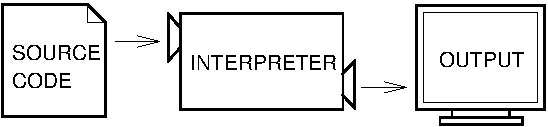
\includegraphics[scale=0.9]{figs/interpret.pdf}}
\caption{Ένας διερμηνέας επεξεργάζετε το πρόγραμμα
λίγο κάθε φορά, αλλίως διαβάζει γραμμές και εκτελεί υπολογισμούς.}
\label{fig.interpret}
\end{figure}

Ένας μεταγλωτιστής διαβάζει το πρόγραμμα και το μεταφράζει ολόκληρο
πριν ξεκινήσει να τρέχει το πρόγραμμα. Σε αυτό το πλαίσιο, το
πρόγραμμα υψηλού επιπέδου ονομάζεται {\bf πηγαίος κώδικας}, και το
μεταφρασμένο πρόγραμμα ονομάζεται {\bf αντικειμενικός κώδικας} ή {\bf εκτελέσιμο}.
Όταν ένα πρόγραμμα μεταγλωτιστεί, μπορείτε να το εκτελέσεται επανειλημμένα
χωρίς περαιτέρω μετάφραση.

Εικόνα~\ref{fig.compile} δείχνει τη δομή ενός μεταγλωτιστή.

\begin{figure}
\centerline
{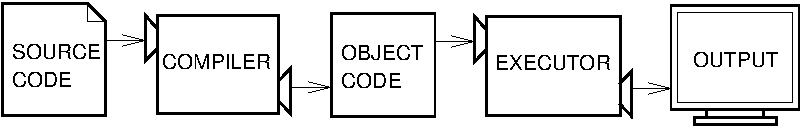
\includegraphics[scale=0.9]{figs/compile.pdf}}
\caption{Ένας μεταγλωττιστής μετατρέπει τον πηγαίο κώδικα σε αντικειμενικό κώδικα, ο οποίος τρέχει από έναν εκτελεστή υλικού.}
\label{fig.compile}
\end{figure}

\gr Η \en Python \gr θεωρείτε μία διερμηνευμένη γλώσσα επειδή τα προγράμματά της
εκτελούνται από έναν διερμηνέα. Υπάρχουν δύο τρόποι χρήσης του διερμηνέα:
{\bf διαδραστική λειτουργία} και{\bf σεναριακή λειτουργία}. Στην διαδραστική
λειτουργία, πληκτρολογούμε προγράμματα σε \en Python \gr και ο διερμηνέας
εμφανίζει το αποτέλεσμα:\en

\index{interactive mode}
\index{script mode}

\begin{verbatim}

>>> 1 + 1
2
\end{verbatim}
%
\gr Το σύμβολο, \en \verb">>>", \gr είναι ο
{\bf προτροπέας} που χρησιμοποιεί ο διερμηνέας για να υποδείξει ότι είναι έτοιμος. Αν
πληκτρολογήσετε {\tt 1 + 1}, ο διερμηνέας απαντάει {\tt 2}.
\index{prompt}

Εναλλακτικά, μπορείτε να αποθηκεύσετε κώδικα σε ένα φάκελο και να χρησιμοποιήσετε
το διερμηνέα για να εκτελέσει τα περιεχόμενα του φακέλου, το οποίο ονομάζεται ένα
{\bf σενάριο}. Κατά παράδοση, τα σενάρια της \en Python \gr έχουν ονόματα τα οποία
έχουν κατάληξη \en {\tt .py}.
\index{script}

\gr Για να εκτελεστεί το σενάριο, πρέπει να πείτε στο διερμηνέα το όνομα
του φακέλου. Εάν έχετε ένα σενάριο με όνομα \en{\tt dinsdale.py} \gr
και δουλεύετε σε ένα παράθυρο εντολών \en UNIX, \gr πληκτρολογείτε \en
{\tt python dinsdale.py}. \gr Σε άλλα περιβάλλοντα ανάπτυξης, οι λεπτομέρειες
εκτέλεσης των σεναρίων είναι διαφορετικές. Μπορείτε να βρείτε οδηγίες για
το περιβάλλον σας στην ιστοσελίδα της \en Python \url{http://python.org}.

\index{testing!interactive mode}

\gr Όταν δουλεύετε στην διαδραστική λειτουργία σας βοηθάει να εξετάζετε
μικρά κομμάτια κώδικα επειδή μπορείτε να τα πληκτρολογήσετε και να εκτελεστούν
άμεσα. Αλλά για κάτι παραπάνω από λίγες γραμμές, θα πρέπει να αποθηκεύσετε τον
κώδικά σας σαν σενάριο ώστε να μπορείτε να τον τροποποιήσετε και να το εκτελέσετε
στο μέλλον.


\section{ Τι είναι ένα πρόγραμμα}

Ένα {\bf πρόγραμμα} είναι μία ακολουθία εντολών η οποία προσδιορίζει
πως θα εκτελεστεί ένας υπολογισμός. Αυτός ο υπολογισμός μπορεί να είναι
κάτι μαθηματικό, όπως το να λύνεις ένα σύστημα εξισώσεων ή το να βρίσκεις
τις ρίζες ενός πολυωνύμου, αλλά επίσης μπορεί να είναι ένας συμβολικός
υπολογισμός, όπως το να ψάχνεις και να αντικαθιστάς κείμενο μέσα σε ένα
έγγραφο ή (περιέργως) να μεταγλωττίζεις ένα πρόγραμμα.

\index{program}
\gr
Οι λεπτομέρειες είναι διαφορετικές σε κάθε γλώσσα, αλλά μερικές βασικές
εντολές εμφανίζονται σχεδόν σε κάθε γλώσσα:

\begin{description}
\item[είσοδος:]   Εισάγονται δεδομένα από το πληκτρολόγιο, ένα αρχείο, ή οποιαδήποτε
άλλη συσκευή.

\item[έξοδος:]   Εμφανίζονται δεδομένα στην οθόνη ή στέλνονται σε κάποιο αρχείο
ή συσκευή.

\item[μαθηματικά:]   Εκτελούνται βασικές μαθηματικές πράξεις όπως πρόσθεση και
πολλαπλασιασμός.

\item[εκτέλεση υπό συνθήκη:]	  Ελέγχονται συγκεκριμένες συνθήκες και εκτελείται
ο κατάλληλος κώδικας.

\item[επανάληψη:]   Εκτελείται κάποια ενέργεια κατ'επανάληψη, με κάποια παραλλαγή.

\end{description}
\gr
Eίτε το πιστεύετε είτε όχι, λίγο πολύ αυτό είναι όλο. Κάθε πρόγραμμα
που έχετε χρησιμοποιήσει, ανεξάρτητα από το πόσο περίπλοκο ήταν,
απαρτίζεται από εντολές που μοιάζουν λίγο πολύ όπως αυτές. Έτσι
μπορείτε να φανταστείτε τον προγραμματισμό σαν μία διαδικασία κατά
την οποία σπάμε μία μεγάλη και πολύπλοκη εργασία σε όλο και μικρότερες
υποδιεργασίες μέχρις ότου οι υποδιεργασίες να είναι αρκετά απλές για
να εκτελεστούν με μία από αυτές τις βασικές εντολές.
\en \index{algorithm}
\gr
Αυτό μπορεί να είναι λίγο ασαφές, αλλά θα επανέλθουμε σε αυτό το θέμα
όταν θα μιλήσουμε για αλγόριθμους.


\section{Τι είναι η αποσφαλμάτωση;}
\index{debugging}
\index{bug}
Ο προγραμματισμός είναι επιρρεπής σε λάθη. Για ανεξήγητους λόγους,
τα λάθη στον προγραμματισμό ονομάζονται στα αγγλικά \en{\bf bugs}
\gr ενώ στα ελληνικά σφάλματα και η διαδικασία εντοπισμού τους ονομάζεται
\en{\bf debugging} \gr ή αποσφαλμάτωση στα ελληνικά.

\index{debugging}
\index{bug}

Τρία είδη λαθών μπορεί να συμβούν σε ένα πρόγραμμα: συντακτικά λάθη,
λάθη χρόνου εκτέλεσης, και λογικά λάθη. Είναι χρήσιμο να γίνει διάκριση
μεταξύ τους προκειμένου να εντοπίζονται γρηγορότερα.

\subsection{Συντακτικά λάθη}
\index{syntax error}
\index{error!syntax}
\index{error message}

Η \en Python \gr μπορεί να εκτελέσει ένα πρόγραμμα μόνο εάν
έχει σωστή σύνταξη, διαφορετικά ο διερμηνέας εμφανίζει μήνυμα
λάθους. Η σύνταξη αφορά τη δομή ενός προγράμματος και τους
κανόνες αυτής της δομής.\index{syntax}
Για παράδειγμα, οι παρενθέσεις πρέπει να είναι πάντα ζεύγη,
έτσι το {\tt (1 + 2)} είναι σωστό, αλλά το {\tt 8)} είναι ένα
συντακτικό λάθος.

\index{parentheses!matching}
\index{syntax}
\index{cummings, e. e.}

Στα Αγγλικά οι αναγνώστες δέχονται τα περισσότερα συντακτικά λάθη,
για αυτό μπορούμε να διαβάζουμε την ποίηση του \en e. e. cummings
\gr χωρίς να αραδιάζουμε μηνύματα λάθους. Η \en Python \gr δεν
είναι τόσο επιεικής. Εάν υπάρχει έστω και ένα συντακτικό λάθος
οπουδήποτε μέσα στο πρόγραμμα, η \en Python \gr θα εμφανίσει ένα
μήνυμα λάθους και θα σταματήσει, και δεν θα μπορείτε να τρέξετε
το πρόγραμμα. Κατά τη διάρκεια των πρώτων εβδομάδων της προγραμματιστικής
σας καριέρας, πιθανότατα θα ξοδέψετε πολύ χρόνο στον εντοπισμό συντακτικών
λαθών. Όσο αποκτάτε εμπειρία θα κάνετε λιγότερα λάθη και θα τα εντοπίζετε
γρηγορότερα.

\subsection{Λάθη χρόνου εκτέλεσης}
\label{runtime}

Ο δεύτερος τύπος λάθους είναι τα λάθη χρόνου εκτέλεσης, ονομάζονται
έτσι επειδή τα λάθη δεν εμφανίζονται μέχρις ότου αρχίσει το πρόγραμμα
να τρέχει. Αυτά τα λάθη ονομάζονται επίσης εξαιρέσεις επειδή συνήθως
υποδεικνύουν ότι κάτι σημαντικό (και κακό) έχει συμβεί.
\index{runtime error}
\index{error!runtime}
\index{exception}
\index{safe language}
\index{language!safe}

Τα λάθη χρόνου εκτέλεσης είναι σπάνια στα απλά προγράμματα που θα δείτε
στα πρώτα κεφάλαια, έτσι ίσως πάρει λίγο χρόνο μέχρι να συναντήσετε ένα.

\subsection{Λογικά λάθη}
\index{semantics}
\index{semantic error}
\index{error!semantic}
\index{error message}

Ο τρίτος τύπος λάθους είναι τα λογικά λάθη. Εάν υπάρχει ένα λογικό
λάθος στο πρόγραμμά σας θα τρέξει επιτυχώς από την άποψη ότι ο υπολογιστής
δεν θα παράξει κανένα μήνυμα λάθους, αλλά δεν θα κάνει το σωστό. Θα
κάνει κάτι διαφορετικό. Συγκεκριμένα, θα κάνει αυτό που του είπατε να
κάνει.

Το πρόβλημα είναι ότι το πρόγραμμα που γράψατε δεν είναι το πρόγραμμα
που θέλατε να γράψετε. Το νόημα του προγράμματος (η σημασιολογία του)
είναι λάθος. Η αναγνώριση λογικών λαθών μπορεί να είναι δύσκολη γιατί
απαιτεί να δουλέψετε προς τα πίσω κοιτάζοντας την έξοδο του προγράμματος
προσπαθώντας να καταλάβετε τι συμβαίνει.

\subsection{Πειραματική αποσφαλμάτωση}

Μία από τις πιο σημαντικές ικανότητες που θα αποκτήσετε είναι
η αποσφαλμάτωση. Παρόλο που μπορεί να είναι μια επίπονη διαδικασία,
η αποσφαλμάτωση είναι ένα από τα πιο πνευματικώς πλούσια, προκλητικά
και ενδιαφέροντα μέρη του προγραμματισμού.

\index{experimental debugging}
\index{debugging!experimental}

Υπό μία έννοια, η αποσφαλμάτωση είναι σαν την δουλειά του ντετέκτιβ.
Έρχεστε αντιμέτωποι με ενδείξεις, και πρέπει να συμπεράνετε από ποιες
διαδικασίες και συμβάντα προκύπτουν τα αποτελέσματα που βλέπετε.

Η αποσφαλμάτωση μοιάζει επίσης σαν μία πειραματική επιστήμη. Από τη στιγμή
που έχετε μία ιδέα για το τι πηγαίνει λάθος, τροποποιείτε το πρόγραμμα και
ξαναδοκιμάζετε. Εάν η υπόθεσή σας ήταν σωστή, τότε μπορείτε να προβλέψετε
το αποτέλεσμα της τροποποίησης, και είστε ένα βήμα πιο κοντά σε ένα
λειτουργικό πρόγραμμα. Εάν η υπόθεσή σας ήταν λανθασμένη, πρέπει να κάνετε
μία νέα υπόθεση. Όπως έχει τονίσει ο \en Sherlock Holmes, \gr "´Οταν έχετε
αποκλείσει το αδύνατο, οτιδήποτε μένει, όσο απίθανο και αν είναι, πρέπει να
είναι η αλήθεια." \en(A. Conan Doyle, {\em The Sign of Four})
\index{Holmes, Sherlock}
\index{Doyle, Arthur Conan}
\gr
Για μερικούς ανθρώπους, ο προγραμματισμός και η αποσφαλμάτωση είναι το ίδιο
πράγμα. Δηλαδή, ο προγραμματισμός είναι η διαδικασία της σταδιακής
αποσφαλμάτωσης ενός προγράμματος εώς ότου κάνει αυτό που θέλετε.
Η γενική ιδέα είναι ότι θα πρέπει να ξεκινάτε με ένα πρόγραμμα το
οποίο κάνει "κάτι" και να κάνετε μικρές τροποποιήσεις, αποσφμαλματώνοντάς τες
προχωρώντας, έτσι ώστε να έχετε πάντα ένα λειτουργικό πρόγραμμα.
Για παράδειγμα, το \en Linux \gr είναι ένα λειτουργικό σύστημα το οποίο
περιέχει χιλιάδες γραμμές κώδικα, αλλά ξεκίνησε σαν ένα απλό πρόγραμμα
το οποίο ο \en Linus Torvalds \gr χρησιμοποιούσε για να εξερευνήσει
το ολοκληρωμένο \en Intel 80386. \gr Σύμφωνα με τον \en Larry Greenfield,
\gr "Μία από τις πρώτες εργασίες του \en Linus \gr ήταν ένα πρόγραμμα
το οποίο θα αντέστρεφε την εκτύπωση από ΑΑΑΑ σε ΒΒΒΒ. Αυτό αργότερα εξελίχθηκε
στο \en Linux."  ({\em The Linux Users' Guide} Beta Version 1).

\index{Linux}
\gr Τα επόμενα κεφάλαια θα κάνουν περισσότερες υποδείξεις σχετικά με την αποσφαλμάτωση και
άλλες προγραμματιστικές πρακτικές.


\section{Επίσημες και φυσικές γλώσσες}
\index{formal language}
\index{natural language}
\index{language!formal}
\index{language!natural}

Οι φυσικές γλώσσες είναι οι γλώσσες που μιλούν οι άνθρωποι,
όπως τα Αγγλικά, τα Ισπανικά και τα Γαλλικά. Δεν έχουν σχεδιαστεί
από τους ανθρώπους (παρόλο που οι άνθρωποι προσπαθούν να επιβάλουν
κάποια τάξη σε αυτές), έχουν εξελιχθεί φυσικά.

Οι επίσημες γλώσσες είναι γλώσσες που έχουν σχεδιαστεί από ανθρώπους
για συγκεκριμένες εφαρμογές. Για παράδειγμα, η σημειογραφία που χρησιμοποιούν
οι μαθηματικοί είναι μια επίσημη γλώσσα η οποία είναι ειδοκότερα καλή στο
να δείχνει τις σχέσεις μεταξύ αριθμών και συμβόλων. Οι χημικοί χρησιμοποιούν
μία επίσημη γλώσσα για να αναπαραστήσουν τη χημική δομή των μορίων. Και το πιο
σημαντικό:

\begin{quote}
{Οι προγραμματιστικές γλώσσες είναι επίσημες γλώσσες οι οποίες έχουν σχεδιαστεί
για να εκφράζουν υπολογισμούς.}
\end{quote}

Οι επίσημες γλώσσες τείνουν να έχουν αυστηρούς κανόνες σύνταξης. Για
παράδειγμα,
$3 + 3 = 6$  είναι μία συντακτικά σωστή μαθηματική έκφραση, αλλά αυτή
$3 + = 3 \mbox{\$} 6$ δεν είναι.
$H_2O$ είναι ένας συντακτικά σωστός
χημικός τύπος,αλλά αυτός $_2Zz$ δεν είναι.

Οι κανόνες σύνταξης είναι δύο τύπων, οι οποίοι αφορούν τα σύμβολα
και τη δομή. Τα σύμβολα είναι τα βασικά στοιχεία της γλώσσας, όπως
λέξεις, αριθμοί και χημικά στοιχεία. Ένα από τα προβλήματα με το
$3 + = 3 \mbox{\$} 6$ είναι ότι το \( \$ \) δεν είναι ένα έγκυρο
σύμβολο στα μαθηματικά (τουλάχιστον όσο γνωρίζω). Παρομοίως, το
$_2Zz$ δεν είναι έγκυρο επειδή δεν υπάρχει στοιχείο με την συντομογραφία
$Zz$.

\index{token}
\index{structure}

Ο δεύτερος τύπος συντατικού κανόνα αφορά τη δομή μίας έκφρασης,
δηλαδή, τον τρόπο με τον οποίο έχουν διαταχθεί τα σύμβολα.
Η έκφραση $3 + = 3$ είναι λάθος γιατί παρόλο που το $+$ και το
$=$ είναι έγκυρα σύμβολα, δεν μπορείτε να έχετε το ένα ακριβώς
μετά το άλλο. Παρομοίως, σε ένα χημικό τύπο ο δείκτης μπαίνει
μετά το όνομα του στοιχείου, όχι πριν.

\begin{exercise}

Γράψτε μία σωστά δομημένη Αγγλική πρόταση με άκυρα σύμβολα.
Έπειτα γράψτε μία άλλη πρόταση με σωστά σύμβολα αλλά με λανθασμένη
δομή.

\end{exercise}

Όταν διαβάζετε μία πρόταση στα Αγγλικά ή μία έκφραση σε μία επίσημη
γλώσσα, πρέπει να καταλάβετε ποια είναι η δομή της πρότασης
(παρόλο που σε μια φυσική γλώσσα το κάνετε υποσυνείδητα). Αυτή
η διαδικασία ονομάζεται συντακτική ανάλυση.
\index{parse}

Για παράδειγμα, όταν ακούτε την πρόταση, "Το νόμισμα έπεσε,"
καταλαβαίνετε ότι "το νόμισμα" είναι το αντικείμενο και "έπεσε"
είναι το κατηγορούμενο. Μόλις αναλύσετε μία πρόταση, μπορείτε
να καταλαβετε τι σημαίνει, ή τη σημασιολογία της πρότασης.
Υποθέτοντας ότι γνωρίζετε τι είναι το νόμισμα και τι σημαίνει το ότι
πέφτει, θα καταλάβετε τον υπαινιγμό της πρότασης.

Παρόλο που οι επίσημες και οι φυσικές γλώσσες έχουν πολλά κοινά
χαρακτηριστικά---σύμβολα, δομή, συντακτικό και σημασιολογία---υπάρχουν
κάποιες διαφορές:
\index{ambiguity}
\index{redundancy}
\index{literalness}

\begin{description}

\item[ασάφεια:] Οι φυσικές γλώσσες είναι γεμάτες ασάφεια, την οποία
οι άνθρωποι αντιμετωπίζουν από τα συμφραζόμενα και άλλες πληροφορίες.
Οι επίσημες γλώσσες έχουν σχεδιαστεί για να είναι σχεδόν ή πλήρως σαφείς,
το οποίο σημαίνει ότι οποιαδήποτε έκφραση έχει ακριβώς μία ερμηνεία,
ανεξαρτήτου περιεχομένου.

\item[πλεονασμός:] Προκειμένου να επιτύχουμε σαφήνεια και να μειώσουμε
τις παρεξηγήσεις,οι φυσικές γλώσσες χρησιμοποιούν πολλούς πλεονασμούς.
Σαν αποτέλεσμα, είναι συχνά φλύαρες. Οι επίσημες γλώσσες είναι λιγότερο
πλεονάζουσες και περισσότερο συνοπτικές.

\item[μεταφορά:] Οι φυσικές γλώσσες είναι γεμάτες από ιδιωματισμούς
και μεταφορές. Εάν πώ, "Το νόμισμα έπεσε," πιθανώς δεν υπάρχει νόμισμα
και τίποτα δεν έχει πέσει (αυτός ο ιδιωματισμός σημαίνει ότι κάποιος
συνηδειτοποίησε κάτι μετά από μία περίοδο συγχυσης). Οι επίσημες γλώσσες
εννοούν αυτό ακριβώς που λένε.

\end{description}

Οι άνθρωποι που μεγάλωσαν μιλώντας μία φυσική γλώσσα---όλοι---τους είναι
συχνά δύσκολο να εξοικειωθούν με τις επίσημες γλώσσες. Κατά κάποιον τρόπο,
η διαφορά ανάμεσα στην επίσημη και στη φυσική γλώσσα είναι σαν τη διαφορά
ανάμεσα στην ποίηση και στον πεζό λόγο, αλλά ειδικότερα:
\index{poetry}
\index{prose}

\begin{description}

\item[Ποίηση:] Οι λέξεις χρησιμοποιούνται τόσο για τους ήχους τους
όσο και για τη σημασία τους, και ολόκληρο το ποίημα δημιουργεί μία
συναισθηματική αντίδραση. Η ασάφεια δεν είναι μόνο σύνηθες φαινόμενο
αλλά συχνά σκόπιμη.

\item[Πεζός λόγος:] Η κυριολεκτική έννοια των λέξεων είναι περισσότερο
σημαντική, και η δομή συμβάλλει περισσότερο στο νόημα. Ο πεζός λόγος
επιδέχεται περισσότερη ανάλυση από την ποίηση αλλά είναι συχνά
διφορούμενος.

\item[Προγράμματα:] Το νόημα ενός υπολογιστικού ποργράμματος είναι
σαφές και κυριολεκτικό, και μπορεί να κατανοηθεί πλήρως μέσω της ανάλυσης
των συμβόλων και της δομής.

\end{description}

Υπάρχουν κάποιες υποδείξεις για να διαβάζετε προγράμματα (και άλλες
επίσημες γλώσσες). Πρώτον, να θυμάστε ότι οι επίσημες γλώσσες είναι
περισσότερο πυκνογραμμένες από τις φυσικές γλώσσες, γι' αυτό παίρνει
περισσότερο να τις διαβάσουμε. Επίσης, η δομή είναι πολύ σημαντική,
οπότε συνήθως δεν είναι καλή ιδέα να τις διαβάζουμε από την αρχή προς
το τέλος, από αριστερά στα δεξιά. Αντί αυτού, πρέπει να μάθετε να αναλύετε
το πρόγραμμα στο μυαλό σας, αναγνωρίζοντας τα σύμβολα και ερμηνεύοντας
τη δομη. Τελικά, οι λεπτομέρειες μετράνε. Μικρά λάθη στο συλλαβισμό και
στη στίξη, τα οποία δεν δημιουργούν σοβαρό πρόβλημα στις φυσικές γλώσσες,
μπορούν να κάνουν μεγάλη διαφορά σε μία επίσημη γλώσσα.


\section{Το πρώτο πρόγραμμα}
\label{hello}
\index{Hello, World}

Κατά παράδοση, το πρώτο πρόγραμμα που γράφετε σε μία νέα
γλώσσα ονομάζεται \en '' Hello, World!'' \gr επειδή το μόνο που κάνει
είναι να εμφανίζει τις λέξεις \en ''Hello, World''. \gr Στην \en Python
\gr φαίνεται κάπως έτσι:
\en
\begin{verbatim}
print 'Hello, World!'
\end{verbatim}
%
\gr
Αυτό είναι ένα παράδειγμα μίας έκφρασης εκτύπωσης, η οποία
στην πραγματικότητα δεν εκτυπώνει κάτι στο χαρτί. Εμφανίζει μία
τιμή στην οθόνη. Σε αυτή την περίπτωση, το αποτέλεσμα είναι οι λέξεις
\en
\begin{verbatim}
Hello, World!
\end{verbatim}
%
\gr
Τα εισαγωγικά μέσα στο πρόγραμμα σηματοδοτούν την αρχή και το τέλος
του κειμένου που θα εμφανιστεί, δεν φαίνονται στο αποτέλεσμα.

\index{quotation mark}
\index{print statement}
\index{statement!print}

Στην \en Python 3, \gr η σύνταξη για εκτύπωση είναι λίγο διαφορετική:
\en
\begin{verbatim}
print('Hello, World!')
\end{verbatim}
%
\gr Οι παρενθέσεις υποδηλώνουν ότι το \en {\tt print} \gr είναι μία
λειτουργία. Θα φτάσουμε  στις λειτουργίες στο Κεφάλαιο~\en \ref{funcchap}.

\index{function} \index{print function} \index{Python 3}
\gr
Στη συνέχεια αυτού του βιβλίου, θα χρησιμοποιώ την έκφραση \en print. \gr
Εάν χρησιμοποιείτε την \en Python 3, \gr θα πρέπει να την προσαρμόζετε.
Αλλά πέρα από αυτό, υπάρχουν πολύ λίγες διαφορές για τις οποίες θα
πρέπει να ανησυχούμε.


\section{Αποσφαλμάτωση}
\index{debugging}
Μια καλή ιδέα είναι να διαβάζετε αυτό το βιβλίο μπροστά από έναν υπολογιστή
έτσι ώστε να μπορείτε να δοκιμάζετε τα παραδείγματα καθώς προχωράτε. Μπορείτε
να τρέξετε τα περισσότερα από τα παραδείγμα σε διαδραστική λειτουργία, αλλά
βάλετε τον κώδικα σε ένα σενάριο, είναι ευκολότερο να δοκιμάσετε παραλλαγές.

Όποτε πειραματίζεστε με ένα νέο χαρακτηριστικό, θα πρέπει να δοκιμάζετε
να κάνετε λάθη. Για παράδειγμα, στο πρόγραμμα \en ''Hello, world!'',
\gr τι θα συμβεί αν δεν βάλετε ένα από τα εισαγωγικά\en; \gr Εάν δεν
βάλετε κανένα από τα δύο\en; \gr Εάν γράψετε λάθος το \en {\tt print};
\index{error message}
\gr
Αυτό το είδος πειραματισμού σας βοηθάει να θυμάστε τι διαβάζετε, και επίσης
σας βοηθάει στην αποσφαλμάτωση, επειδή θα μάθετε τι σημαίνουν τα μηνύματα
λάθους. Είναι προτιμότερο να κάνετε εσκεμμένα λάθη τώρα παρά αργότερα κατά
λάθος.

Ο προγραμματισμός, και ιδιαίτερα η αποσφαλμάτωση, μερικές φορές προκαλεί
έντονα συναισθήματα. Εάν ταλαιπωρείστε με ένα δύσκολο σφάλμα, μπορεί να
νιώσετε θυμωμένοι, αποθαρρυμένοι ή ντροπιασμένοι.

Υπάρχει απόδειξη ότι οι άνθρωποι ανταποκρίνονται φυσικά στους υπολογιστές
σαν να ήταν άνθρωποι. Όταν λειτουργούν σωστά, τους βλέπουμε σαν συνεργάτες,
και όταν είναι πεισματάρηδες ή αγενείς, συμπεριφερόμαστε σε αυτούς με τον
ίδιο τρόπο που θα συμπεριφερόμασταν σε αγενείς και πεισματάρηδες ανθρώπους
\en (Reeves and Nass, {\it The Media
    Equation: How People Treat Computers, Television, and New Media
    Like Real People and Places}).
\index{debugging!emotional response}
\index{emotional debugging}
\gr
Το να είστε προετοιμασμένοι για αυτές τις αντιδράσεις μπορεί να
σας βοηθήσει να τις αντιμετωπίσετε. Μία προσέγγιση είναι να σκέφτεστε
τον υπολογιστή σαν ένα υπάλληλο με συγκεκριμένες δυνατότητες, όπως
η ταχύτητα και η ακρίβεια και συγκεκριμένες αδυναμίες, όπως η έλλειψη
συναίσθησης και η ανικανότητά τους να κατανοήσουν το γενικό νόημα.

Η δουλειά σας είναι να είστε ένας καλός διευθυντής: βρείτε τρόπους
να εκμεταλευτείτε τις δυνατότητες και να μετριάσετε τις αδυναμίες.
Επίσης, βρείτε τρόπους να χρησιμοποιήσετε τα συναισθήματά σας ώστε
να ασχοληθείτε με το πρόβλημα, χωρίς να αφήσετε τις αντιδράσεις σας
να επηρεάσουν την ικανότητά σας να δουλεύτε αποδοτικά.

Το να μάθαιτε να αποσφαλματώνετε μπορεί να είναι απογοητευτικό,
αλλά είναι μία σημαντική ικανότητα η οποία είναι χρήσιμη και για
πολλές δραστηριότητες πέραν του προγραμματισμού. Στο τέλος κάθε
κεφαλαίου υπάρχει μία ενότητα αποσφαλμάτωσης, όπως αυτή, με τις
σκέψεις μου σχετικά με την αποσφαλμάτωση. Ελπίζω να βοηθήσουν!


\section{Ορολογία}

\begin{description}

\item[επίλυση προβλημάτων:]  Η διαδικασία τυποποίησης ενός προβλήματος,
	η εύρεση λύσης και η έκφραση της λύσης.
\index{problem solving}

\item[γλώσσα υψηλού επιπέδου:]  Μία γλώσσα προγραμματισμού όπως η \en
	Python \gr που έχει σχεδιαστεί για να είναι εύκολη για τους ανθρώπους
	στην ανάγνωση και στη γραφή.
\index{high-level language}

\item[γλώσσα χαμηλού επιπέδου:]  Μία γλώσσα που έχει σχεδιαστεί για να είναι
	εύκολο να εκτελεστεί από έναν υπολογιστή, ονομάζεται επίσης "γλώσσα μηχανής" ή
	"συμβολική γλώσσα."
\index{low-level language}

\item[φορητότητα:]  Η ιδιότητα ενός προγράμματος να μπορεί να τρέξει σε
	σε διαφορετικούς υπολογιστές.
\index{portability}

\item[διερμηνεία:]  Να εκτελείς ένα πρόγραμμα γλώσσας υψηλού επιπέδου
	μεταφράζοντάς μία γραμμή κάθε φορά.
\index{interpret}

\item[μεταγλώττιση:]  Να μεταφράζεις ένα πρόγραμμα γραμμένο σε γλώσσα
	υψηλού επιπέδου σε γλώσσα χαμηλού επιπέδου κατευθείαν, προετοιμάζοντάς το
	για μετέπειτα εκτέλεση.
\index{compile}

\item[πηγαίος κώδικας:]  Ένα πρόγραμμα σε μία γλώσσα υψηλού επιπέδου
	προτού μεταγλωττιστεί.
\index{source code}

\item[αντικειμενικός κώδικας:]  Η έξοδος του μεταγλωττιστή αφού μετατρέψει
	το πρόγραμμα.
\index{object code}

\item[εκτελέσιμο:]  Μία άλλη ονομασία του αντικειμενικού κώδικα ο οποίος
	είναι έτοιμος για εκτέλεση.
\index{executable}

\item[προτροπέας:] Οι χαρακτήρες που εμφανίζονται από το διερμηνέα για
	υποδηλώσουν ότι είναι έτοιμος να δεχτεί την είσοδο από το χρήστη.
\index{prompt}

\item[σενάριο:] Ένα πρόγραμμα αποθηκευμένο σε ένα αρχείο (συνήθως προς
	διερμηνεία).
\index{script}

\item[διαδραστική λειτουργία:] Ένας τρόπος χρήσης του διερμηνέα της
	\en Python \gr πληκτρολογώντας εντολές και εκφράσεις στον προτροπέα.
\index{interactive mode}

\item[λειτουργία σεναρίου:] Ένας τρόπος χρήσης του διερμηνέα της \en
	Python \gr που διαβάζει και εκτελεί εκφράσεις σε ένα σενάριο.
\index{script mode}

\item[πρόγραμμα:] Ένα σύνολο εντολών που ορίζει έναν υπολογισμό.
\index{program}

\item[αλγόριθμος:]  Μία γενική διαδικασία για την επίλυση μιας κατηγορίας
	προβλημάτων.
\index{algorithm}

\item[σφάλμα:]  Ένα λάθος σε ένα πρόγραμμα.
\index{bug}

\item[αποσφαλμάτωση:]  Η διαδικασία της εύρεσης και αφαίρεσης οποιουδήποτε
	εκ των τριών τύπων προγραμματιστικών σφαλμάτων.
\index{debugging}

\item[συντακτικό:]  Η δομή ενός προγράμματος.
\index{syntax}

\item[συντατκικό λάθος:]  Ένα λάθος σε ένα πρόγραμμα το οποίο το καθιστά
	αδύνατο να αναλυθεί (και επομένως αδύνατον να διερμηνευτεί).
\index{syntax error}

\item[εξέρεση:]  Ένα λάθος το οποίο ανιχνεύεται ενώ το πρόγραμμα τρέχει.
\index{exception}

\item[σημασιολογία:]  Το νόημα ενός προγράμματος.
\index{semantics}

\item[σημασιολογικό λάθος:]   Ένα λάθος σε ένα πρόγραμμα το οποίο το κάνει
	να κάνει κάτι διαφορετικό από αυτό που είχε σκοπό ο προγραμματιστείς να κάνει.
\index{semantic error}

\item[φυσική γλώσσα:]  Οποιαδήποτε από τις γλώσσες που μιλούν οι άνθρωποι
	η οποία έχει εξελιχθεί φυσικά.
\index{natural language}

\item[επίσημη γλώσσα:]  Οποιαδήποτε από τις γλώσσες που έχουν σχεδιάσει
	οι άνθρωποι για συγκεκριμένους σκοπούς, όπως αναπαράσταση μαθηματικών
	ιδεών ή προγραμμάτων υπολογιστών. Όλες οι γλώσσες προγραμματισμού είναι
	επίσημες γλώσσες.
\index{formal language}

\item[σύμβολο:]  Ένα από τα βασικά στοιχεία της συντακτικής δομής ενός
	προγράμματος, ανάλογο με τη λέξη σε μια φυσική γλώσσα.
\index{token}

\item[ανάλυση:] Να εξετάζεις ένα πρόγραμμα και να αναλύεις την συντακτική
	του δομή.
\index{parse}

\item[εκτύπωση έκφρασης:]  Μία εντολή που προκαλεί τον διερμηνέα της \en
	Python \gr να εμφανίσει μία τιμή στην οθόνη.
\index{print statement}
\index{statement!print}


\end{description}


\section{Ασκήσεις}

ΑΣΚΗΣΗ 1η

Χρησιμοποιήστε ένα φυλλομετρητή για να επισκεφθείτε την ιστοσελίδα της
\en Python \url{http://python.org}.\gr
Αυτή η σελίδα περιέχει πληροφορίες σχετικά με την \en Python \gr
και συνδέσμους οι οποίοι σχετίζονται με την \en Python, \gr
και σας δίνει την δυνατότητα να αναζητήσετε την τεκμηρίωση της \en Python.
\gr
Για παράδειγμα, εάν πληκτρολογήσετε \en {\tt print} \gr στο πεδίο της
αναζήτησης, ο πρώτος σύνδεσμος που εμφανίζεται είναι η τεκμηρίωση για αυτήν
την έκφραση. Σε αυτό το σημείο, δεν θα βγάζει όλο αυτό νόημα σε εσάς,
αλλά είναι καλό να ξέρετε που υπάρχει.
\index{documentation}
\index{python.org}


ΑΣΚΗΣΗ 2η

Εκκινήστε τον διερμηνέα της \en Python \gr πληκτρολογίστε \en {\tt help()} \gr
για να ξεκινήσει το διαδικτυακό εργαλείο βοήθειας. Ή μπορείτε να πληκτρολογήσετε
\en \verb"help('print')" \gr για να πάρετε πληροφορίες σχετικές με την πρόταση
\en {\tt print}.
\gr
Εάν αυτό το παράδειγμα δεν δουλεύει, ίσως χρειαστεί να εγκαταστήσετε επιπρόσθετη
τεκμηρίωση της \en Python \gr ή να θέσετε μία μεταβλητή περιβάλλοντος, οι λεπτομέρειες
εξαρτώνται από το λειτουργικό σας σύστημα και την έκδοση της \en Python. \gr
\index{help utility}


ΑΣΚΗΣΗ 3η

Εκκινήστε τον διερμηνέα της \en Python \gr και χρησιμοποιήστε τον
σαν αριθμομηχανή. Το συντακτικό της \en Python \gr για μαθηματικές
πράξεις είναι σχεδόν το ίδιο με την τυπική μαθηματική σημειογραφία.
Για παράδειγμα, τα σύμβολα \en {\tt +}, {\tt -} \gr και \en {\tt /}
\gr δηλώνουν πρόσθεση, αφαίρεση και διαίρεση, όπως θα περιμένατε.
Το σύμβολο του πολλαπλασιασμού είναι \en {\tt *}.
\gr
Εάν τρέξετε έναν αγώνα 10 χιλιομέτρων σε 43 λεπτά και 30 δευτερόλεπτα,
ποιός είναι ο μέσος χρόνος σας ανά μίλι; Ποιά είναι η μέση σας ταχύτητα
σε μίλια ανά ώρα; (Σημείωση: ένα μίλι είναι 1,61 χιλιόμετρα).
\index{calculator}
\index{running pace}






\chapter{Μεταβλητές, εκφράσεις and δηλώσεις}

\section{Τιμές και τύποι}
\index{value}
\index{type}
\index{string}

Μία τιμή  είναι ένα από τα βασικά πράγματα με τα οποία δουλεύει
ένα πρόγραμμα, όπως ένα γράμμα ή ένας αριθμός. Οι τιμές που έχουμε
δει μέχρι στιγμής είναι {\tt 1}, {\tt 2}, και \en \verb"'Hello, World!'".

\gr
Αυτές οι τιμές ανήκουν σε διαφορετικούς τύπους:
το {\tt 2} είναι ακέραιος, και το \en \verb"'Hello, World!'" \gr είναι
μία συμβολοσειρά, ονομάζεται έτσι επειδή περιέχει μια "σειρά" από
γράμματα. Μπορείτε (και ο διερμηνέας) να αναγνωρίσετε συμβολοσειρές,
επειδή περικλείονται σε εισαγωγικά.
\index{quotation mark}

Αν δεν είστε σίγουροι για τον τύπο μιας τιμής, μπορεί να σας πει ο διερμηνέας.
\en
\begin{verbatim}
>>> type('Hello, World!')
<type 'str'>
>>> type(17)
<type 'int'>
\end{verbatim}
%
\gr

Προφανώς, οι συμβολοσειρές ανήκουν στον τύπο \en {\tt str}
\gr και οι ακέραιοι ανήκουν στον τύπο \en {\tt int}. \gr
Λιγότερο προφανές είναι, ότι οι αριθμοί με δεκαδικά ψηφία ανήκουν
σε ένα τύπο που ονομάζεται \en {\tt float}, \gr επειδή αυτοί οι αριθμοί
παριστάνονται σε μία μορφή ονομαζόμενη \en {\bf floating-point}.
\index{type}
\index{string type}
\index{type!str}
\index{int type}
\index{type!int}
\index{float type}
\index{type!float}

\begin{verbatim}
>>> type(3.2)
<type 'float'>
\end{verbatim}
%
\gr Τι γίνεταιμε τιμές όπως η \en \verb"'17'" \gr και η \en
\verb"'3.2'"; \gr Μοιάζουν με αριθμούς, αλλά περικλείονται
σε εισαγωγικά όπως οι συμβολοσειρές.
\index{quotation mark}
\en
\begin{verbatim}
>>> type('17')
<type 'str'>
>>> type('3.2')
<type 'str'>
\end{verbatim}
%
\gr
Είναι συμβολοσειρές.

Όταν πληκτρολογείτε έναν μεγάλο ακέραιο, ίσως μπείτε στον πειρασμό
να χρησιμοποιήσετε κόμματα ανά τρία ψηφία, όπως για παράδειγμα
{\tt 1,000,000}. Αυτός δεν είναι ένας έγκυρος ακέραιος στην
\en Python, \gr αλλά γενικότερα είναι έγκυρο:\en

\begin{verbatim}
>>> 1,000,000
(1, 0, 0)
\end{verbatim}
%
\gr
Λοιπόν, αυτό δεν έχει καμία σχέση με αυτό που περιμέναμε! Η \en
Python \gr ερμηνέυει το \en {\tt 1,000,000} \gr σαν μία ακολουθία
ακεραίων χωρισμένη με κόμματα. Αυτό είναι το πρώτο παράδειγμα σημασιολογικού
λάθους που έχουμε δει: ο κώδικας τρέχει χωρίς να παράγει κανένα μήνυμα
λάθους, αλλά δεν κάνει το \en"\gr σωστο\en" \gr πράγμα.

\index{semantic error}
\index{error!semantic}
\index{error message}



\section{Μεταβλητές}
\label{variables}
\index{variable}
\index{assignment statement}
\index{statement!assignment}
Ένα από τα πιο δυνατά χαρακτηριστικά μιας γλώσσας προγραμματισμού
είναι η ικανότητα να διαχειρίζεται μεταβλητές. Μία μεταβλητή είναι
ένα όνομα που αναφέρεται σε μία τιμή.

Μία έκφραση εκχώρησης δημιουργεί νέες μεταβλητές και δίνει τιμές
σε αυτές:
\en
\begin{verbatim}
>>> message = 'And now for something completely different'
>>> n = 17
>>> pi = 3.1415926535897932
\end{verbatim}
%
\gr
Σε αυτό το παράδειγμα κάνουμε τρεις εκχωρήσεις τιμής. Η πρώτη εκχωρεί
μία συμβολοσειρά σε μία νέα μεταβλητή με όνομα \en  {\tt message}, \gr
η δεύτερη δίνει τον ακέραιο \en {\tt 17} \gr στη \en {\tt n}, \gr και
η τρίτη εκχωρεί την (κατά προσέγγιση) τιμή του $\pi$ στην \en {\tt pi}.
\index{state diagram}
\index{diagram!state}
\gr
Ένας σύνηθες τρόπος αναπαράστασης μεταβλητών σε χαρτί είναι να γράψετε το
όνομα με ένα βελάκι το οποίο δείχνει την τιμή της μεταβλητής. Αυτός ο τρόπος
απεικόνισης ονομάζεται διάγραμμα κατάστασης, γιατί δείχνει την κατάσταση της
κάθε μεταβλητής.
Το σχήμα~\ref{fig.state2} δείχνει το αποτέλεσμα του προηγούμενου παραδείγματος.

\begin{figure}
\centerline
{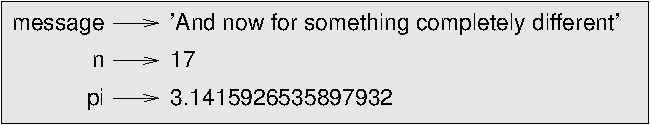
\includegraphics[scale=0.8]{figs/state2.pdf}}
\caption{Διάγραμμα Κατάστασης.}
\label{fig.state2}
\end{figure}

Ο τύπος της μεταβλητής είναι ο τύπος της τιμής στην οποία αναφέρεται.
\en
\begin{verbatim}
>>> type(message)
<type 'str'>
>>> type(n)
<type 'int'>
>>> type(pi)
<type 'float'>
\end{verbatim}

\gr Άσκηση 2.1

Εάν πληκτρολογήσετε έναν ακέραιο που έχει στην αρχή μηδέν, ενδεχομένως
να έχετε ένα λάθος λόγω σύγχυσης στο διερμηνέα:
\en
\begin{verbatim}
>>> zipcode = 02492
                  ^
SyntaxError: invalid token
\end{verbatim}
\gr
Άλλα νούμερα φαίνεται να δουλεύουν, αλλά τα αποτελέσματα είναι παράξενα:
\en
\begin{verbatim}
>>> zipcode = 02132
>>> zipcode
1114
\end{verbatim}
\gr
Μπορείτε να καταλαβέτε τι συμβαίνει\en ; \gr Σημείωση: εμφανίστε τις
τιμές \en {\tt 01}, {\tt 010}, {\tt 0100} \gr και \en {\tt 01000}.
\index{octal}


\gr

\section{Ονόματα μεταβλητών και λέξεις κλειδιά}
\index{keyword}

Γενικά, οι προγραμματιστές επιλέγουν ονόματα για τις μεταβλητές τους
τα οποία έχουν κάποιο νόημα---τεκμηριώνουν για ποιο λόγο χρησιμοποιείται
η μεταβλητή.

Τα ονόματα των μεταβλητών μπορουν να είναι αυθαίρετα μεγάλα.
Μπορούν να περιέχουν και γράμματα και νούμερα, αλλά πρέπει να
ξεκινάνε με ένα γράμμα. Είναι έγκυρο να χρησιμοποιούμε κεφαλαία
γράμματα αλλά είναι προτιμότερο να ξεκινάτε τα ονόματα των μεταβλητών
με πεζά (θα δείτε αργότερα γιατί).

Η κάτω παύλα, \en \verb"_" \gr μπορεί να εμφανιστεί σε ένα όνομα.
Συχνά χρησιοποιείται σε ονόματα με πολλές λέξεις, όπως το \en
\verb"my_name" \gr ή το \en \verb"airspeed_of_unladen_swallow".
\gr
\index{underscore character}

Εάν δώσετε σε μία μεταβλητή λάθος όνομα θα πάρετε ένα συντακτικό λάθος.
\en
\begin{verbatim}
>>> 76trombones = 'big parade'
SyntaxError: invalid syntax
>>> more@ = 1000000
SyntaxError: invalid syntax
>>> class = 'Advanced Theoretical Zymurgy'
SyntaxError: invalid syntax
\end{verbatim}
%
\gr Το \en {\tt 76trombones} \gr είναι λάθος γιατί δεν ξεκινάει με γράμμα.
Το \en {\tt more@} \gr είναι λάθος γιατί περιέχει ένα μη έγκυρο χαρακτήρα, \en {\tt
@}. \gr Αλλά τι είναι λάθος με το \en {\tt class};
\gr
Αποδεικνύεται ότι το \en {\tt class} \gr είναι μία από τις λέξεις κλειδιά της
\en Python. \gr Ο διερμηνέας χρησιμοποιεί λέξεις κλειδιά για να αναγνωρίσει τη δομή ενός
προγράμματος, και για αυτόν το λόγο δεν μπορούν χρησιμοποιηθούν για ονόματα μεταβλητών.

\index{keyword}

Η \en Python 2 \gr έχει 31 λέξεις κλειδιά.
\en
\begin{verbatim}
and       del       from      not       while
as        elif      global    or        with
assert    else      if        pass      yield
break     except    import    print
class     exec      in        raise
continue  finally   is        return
def       for       lambda    try
\end{verbatim}
%
\gr
Στην \en Python 3, \gr το \en {\tt exec} \gr δεν είναι πλέον λέξη κλειδί, αλλά το \en
{\tt nonlocal} \gr είναι.

Ίσως θα θέλατε να έχετε αυτή τη λίστα εύκαιρη. Εάν ο διερμηνέας παραπονιέται για
μία από τις μεταβλητές σας και δεν ξέρετε γιατί, κοιτάξτε αν βρίσκεται σε αυτή τη
λίστα.


\section{Τελεστές και τελεστέοι}
\index{operator, arithmetic}
\index{arithmetic operator}
\index{operand}
\index{expression}

Οι τελεστές είναι ειδικά σύμβολα τα οποία αναπαριστούν υπολογισμούς
όπως η πρόσθεση και ο πολλαπλασιασμός. Οι τιμές στις οποίες εφαρμόζεται
ο τελεστής ονομάζονται τελεστέοι.

Οι τελεστές \en {\tt +}, {\tt -}, {\tt *}, {\tt /} \gr και \en {\tt **}
\gr εκτελούν πρόσθεση, αφαίρεση, πολλαπλασιασμό, δίαιρεση και ύψωση σε
δύναμη, όπώς στα παραδείγματα που ακολουθούν:
\en

\begin{verbatim}
20+32   hour-1   hour*60+minute   minute/60   5**2   (5+9)*(15-7)
\end{verbatim}
%
\gr
Σε κάποιες άλλες γλώσσες, για την ύψωση σε δύναμη χρησιμοποιείται το
σύμβολο \en \verb"^", \gr αλλά στην \en Python \gr είναι δυαδικός
τελεστής και ονομάζεται \en XOR. \gr Σε αυτό το βιβλίο δεν θα επεκταθούμε
στους δυαδικούς τελεστές, αλλά μπορείτε να διαβάσετε για αυτούς στην
διεύθυνση \en \url{http://wiki.python.org/moin/BitwiseOperators} .
\index{bitwise operator}
\index{operator!bitwise}
\gr
Στην \en Python \gr, ο τελεστής της διαίρεσης μπορεί να μην κάνει
αυτό που θα περιμένατε:
\en
\begin{verbatim}
>>> minute = 59
>>> minute/60
0
\end{verbatim}
%
\gr
Η τιμή του \en {\tt minute} \gr είναι 59, και στα συμβατικά μαθηματικά
το 59 διαιρούμενο με το 60 μας δίνει 0.98333, και όχι 0. Ο λόγος που
συμβαίνει αυτό είναι ότι η \en Python \gr εκτελεί ακέραια διαίρεση.
Όταν και οι δύο τελεστέοι είναι ακέραιοι αριθμοί, το αποτέλεσμα είναι
επίσης ακέραιος αριθμός, γιατί η ακέραια διαίρεση κόβει το κλασματικό
τμήμα. Έτσι, σε αυτό το παράδειγμα, το αποτέλεσμα στρογγυλοποιείται
στο μηδέν.


Στην \en Python 3, \gr το αποτέλεσμα της διαίρεσης είναι \en {\tt float}. \gr
Ο νέος τελεστής για την ακέραια διαίρεση είναι \en {\tt //}.
\index{Python 3}
\index{floor division}
\index{floating-point division}
\index{division!floor}
\index{division!floating-point}
\gr
Εάν κάποιος από τους τελεστέους είναι αριθμός κινητής υποδιαστολής,
η \en Python \gr εκτελεί κλασματική διαίρεση, και το αποτέλεσμα είναι
\en {\tt float}:

\begin{verbatim}
>>> minute/60.0
0.98333333333333328
\end{verbatim}

\gr
\section{Εκφράσεις και δηλώσεις}

Μία έκφραση είναι ένας συνδιασμός από τιμές, μεταβλητές και τελεστές.
Μία τιμή από μόνη της θεωρείται σαν μία έκφραση, το ίδιο και μία
μεταβλητή. Έτσι, όλες οι ακόλουθες εκφράσεις είναι έγκυρες
(υποθέτοντας ότι στη μεταβλητή \en {\tt x} \gr έχει ανατεθεί μία τιμή): 				
\index{expression}
\index{evaluate}
\en
\begin{verbatim}
17
x
x + 17
\end{verbatim}
%
\gr
Μία δήλωση είναι μία μονάδα κώδικα την οποία ο διερμηνέας της \en Python
\gr μπορεί να εκτελέσει. Έχουμε δει δύο τύπους δηλώσεων: την εκτύπωση
και την εκχώρηση.

Πρακτικά, μία έκφραση είναι επίσης μία δήλωση, αλλά είναι ίσως πιο
απλό να τα σκέφτεστε σαν δύο διαφορετικά πράγματα. Η σημαντική διαφορά
είναι ότι μία έκφραση έχει μία τιμή, ενώ μία δήλωση όχι.


\section{Διαδραστική λειτουργία και λειτουργία σεναρίων}

Ένα από τα πλεονεκτήματα του να δουλεύεις με μια διερμηνευόμενη γλώσσα
είναι ότι μπορείτε να ελέγχετε μικρά κομμάτια κώδικα στην διαδραστική
λειτουργία πριν τα τοποθετήσετε σε ένα σενάριο. Αλλά υπάρχουν διαφορές
μεταξύ της διαδραστικής λειτουργίας και της λειτουργίας σεναρίων οι οποίες
μπορεί να προκαλέσουν σύγχυση.
\index{interactive mode}
\index{script mode}

Για παράδειγμα, εάν χρησιμοποείτε την \en Python \gr σαν αριθμομηχανή,
μπορεί να πληκτρολογήσετε:
\en
\begin{verbatim}
>>> miles = 26.2
>>> miles * 1.61
42.182
\end{verbatim}
\gr
Στην πρώτη γραμμή εκχωρείται μία τιμή στην \en {\tt miles} \gr, αλλά
δεν έχει κάποια ορατή επίδραση. Η δεύτερη γραμμή είναι μία έκφραση,
επομένως ο διερμηνέας την αποτιμά και εμφανίζει το αποτέλεσμα. Μαθαίνουμε
λοιπόν, ότι ένας μαραθώνιος είναι περίπου 42 χιλιόμετρα.

Αλλά αν πληκτρολογήσετε τον ίδιο κώδικα μέσα σε ένα σενάριο και το
τρέξετε, δεν θα έχετε καμία έξοδο. Σε λειτουργία σεναρίων μία έκφραση,
από μόνη της, δεν έχει καμία ορατή επίδραση. Η \en Python \gr αποτιμά
την έκφραση, αλλά δεν εμφανίζει την τιμή εκτός και αν της πείτε να το κάνει:

\en
\begin{verbatim}
miles = 26.2
print miles * 1.61
\end{verbatim}
\gr
Αυτή η συμπεριφορά μπορεί να σας μπερδεύει στην αρχή.

Ένα σενάριο συνήθως περιέχει μία ακολουθία από δηλώσεις. Εάν
υπάρχουν περισσότερες από μία δήλωση, τα αποτελέσματα εμφανίζονται
ένα κάθε φορά όπως εκτελούνται οι δηλώσεις.

Για παράδειγμα, το σενάριο
\en
\begin{verbatim}
print 1
x = 2
print x
\end{verbatim}
%
\gr
παράγει την έξοδο
\en
\begin{verbatim}
1
2
\end{verbatim}
%
\gr
Η δήλωση εκχώρησης δεν παράγει καμία έξοδο.

ΑΣΚΗΣΗ 2.1

Πληκτρολογήστε τις ακόλουθες δηλώσεις στον διερμηνέα της \en Python \gr
για να δείτε τι κάνουν:

\en
\begin{verbatim}
5
x = 5
x + 1
\end{verbatim}
%
\gr
Τώρα τοποθετήστε τις ίδιες δηλώσεις μέσα σε ένα σενάριο και τρέξτε το.
Ποια είναι η έξοδος; Τροποποιήστε το σενάριο μετατρέποντας καθεμία από
τις εκφράσεις σε μία δήλωση εκτύπωσης και μετά ξανατρέξτε το.


\section{Η σειρά των πράξεων}
\index{order of operations}
\index{rules of precedence}
\index{PEMDAS}
Όταν περισσότεροι από έναν τελεστή εμφανίζονται σε μία έκφαρση,
η σειρά των πράξεων εξαρτάται από τους κανόνες προτεραιότητας.
Για μαθηματικούς τελεστές, η \en Python \gr ακολουθεί την πρότυπη
μαθηματική προτεραιότητα. Ένας χρήσιμος τρόπος για να θυμάστε τους
κανόνες είναι το ακρωνύμιο \en {\bf PEMDAS} :
\index{parentheses!overriding precedence}
\gr
\begin{itemize}

\item Οι παρανθέσεις \en ({\bf P}arentheses) \gr έχουν την υψηλότερη προτεραιότητα και μπορούν
να χρησιμοποιηθούν για να εξαναγκάσουν μια έκφραση να αποτιμηθεί με
τη σειρά που θέλετε. Από τη στιγμή που εκφράσεις στις παρενθέσεις
αξιολογούνται πρώτες, το \en {\tt 2 * (3-1)} \gr μας κάνει 4, και το
\en {\tt (1+1)**(5-2)} \gr μας κάνει 8. Μπορείτε επίσης να χρησιμοποιήσετε
τις παρενθέσεις για να κάνετε μία έκφραση πιο ευανάγνωστη, όπως την \en
{\tt (minute * 100) / 60}, \gr ακόμα και αν δεν αλλάζει το αποτέλεσμα.

\item
Η ύψωση σε δύναμη({\bf E}xponentiation) έχει την αμέσως υψηλότερη
προτεραιότητα, έτσι \en {\tt 2**1+1} \gr κάνει 3, όχι 4, και \en {\tt 3*1**3}
\gr κάνει 3, όχι 27.

\item Ο πολλαπλασιασμός \en ({\bf M}ultiplication) \gr
και η διαίρεση \en {\bf D}ivision) \gr έχουν την ίδια προτεραιότητα,
η οποία είναι υψηλότερη από την πρόσθεση \en ({\bf A}ddition) \gr και
την αφαίρεση \en ({\bf S}ubtraction), \gr οι οποίες έχουν επίσης την
ίδια προτεραιότητα. Έτσι, \en  {\tt 2*3-1} \gr μας κάνει 5, όχι 4, και
\en {\tt 6+4/2}, \gr κάνει 8, όχι 5.

\item Οι τελεστές με την ίδια προτεραιότητα αξιολογούνται από τα
αριστερά στα δεξιά (εκτός της ύψωσης σε δύναμη). Έτσι στην έκφραση
\en {\tt degrees / 2 * pi}, \gr πρώτα γίνεται η διαίρεση και το αποτέλεσμά
της πολλαπλασιάζεται με \en {\tt pi}. \gr Για να διαιρέσετε με $2 \pi$,
μπορείτε να χρησιμοποιήσετε παρενθέσεις ή να γράψετε \en {\tt degrees / 2 / pi}.

\end{itemize}
\gr
Δεν προσπαθώ ιδιαίτερα να θυμάμαι τους κανόνες προτεραιότητας για
άλλους τελεστές. Εάν δεν μπορώ να καταλάβω κοιτώντας την έκφραση,
χρησιμοποιώ παρανθέσεις για να το κάνω ξεκάθαρο.

\section{Πράξεις συμβολοσειρών}
\index{string!operation}
\index{operator!string}

Γενικά, δεν μπορείτε να εκτελέσετε μαθηματικές πράξεις στις συμβολοσειρές,
ακόμα και αν οι συμβολοσειρές μοιάζουν με αριθμούς, οπότε τα ακόλουθα είναι
λάθος:

\en
\begin{verbatim}
'2'-'1'    'eggs'/'easy'    'third'*'a charm'
\end{verbatim}
%
\gr
Ο τελεστής \en {\tt +} \gr δουλεύει με συμβολοσειρές,
αλλά μπορεί να μην κάνει αυτό που περιμένετε: εκτελεί
συνένωση, το οποίο σημαίνει ότι ενώνει τις συμβολοσειρές
τοποθετώντας στο τέλος της πρώτης την αρχή της δεύτερης.
Για παράδειγμα:
\index{concatenation}
\en
\begin{verbatim}
first = 'throat'
second = 'warbler'
print first + second
\end{verbatim}
%
\gr
Η έξοδος αυτού του προγράμματος είναι \en {\tt throatwarbler}.

\gr
Ο τελεστής \en  {\tt *} \gr λειτουργεί επίσης στις συμβολοσειρές, εκτελεί
επανάληψη. Για παράδειγμα,το \en \verb"'Spam'*3" \gr είναι \en \verb"'SpamSpamSpam'".
\gr Εάν ένας από τους τελεστέους είναι συμβολοσειρά, ο άλλος πρέπει να είναι ακέραιος.

Αυτή η χρήση του \en {\tt +} \gr και του \en {\tt *} \gr έχει ανάλογη
σημασία με την πρόσθεση και τον πολλαπλασιασμό. Όπως το \en {\tt 4*3}
\gr είναι ισοδύναμο με το \en {\tt 4+4+4}, \gr περιμένουμε το \en
\verb" 'Spam'*3" \gr να είναι το ίδιο με το \en \verb"'Spam'+'Spam'+'Spam'",
\gr και έτσι είναι. Από την άλλη, υπάρχει μία συγκεκριμένη περίπτωση
στην οποία η συνένωση και η επανάληψη συμβολοσειρών είναι διαφορετικές
από την πρόσθεση και τον πολλαπλασιασμό ακεραίων. Μπορείτε να σκεφτείτε
μία ιδιότητα την οποία έχει η πρόσθεση αλλά όχι η συνένωση συμβολοσειρών\en ;
\index{commutativity}

\gr
\section{Σχόλια}
\index{comment}

Καθώς τα προγράμματα γίνονται μεγαλύτερα και πιο πολύπλοκα, γίνονται
περισσότερο δυσανάγνωστα. Οι επίσημες γλώσσες είναι πυκνογραμμένες,
και είναι συχνά δύσκολο να κοιτάξεις ένα κομμάτι του κώδικα και να
καταλάβεις τι κάνει, ή γιατί.

Για αυτό το λόγο, είναι καλή ιδέα να προσθέτετε σημειώσεις στα προγράμματά σας
για να εξηγείτε σε φυσική γλώσσα τι κάνει το πρόγραμμα. Αυτές οι σημειώσεις
ονομάζονται σχόλια, και ξεκινάνε με το σύμβολο \en \verb"#" :

\begin{verbatim}
# compute the percentage of the hour that has elapsed
percentage = (minute * 100) / 60
\end{verbatim}
%
\gr
Σε αυτή τη περίπτωση, το σχόλιο εμφανίζεται σε μία γραμμή μόνο του. Μπορείτε
επίσης να βάζετε σχόλια και στο τέλος μίας γραμμής:
\en
\begin{verbatim}
percentage = (minute * 100) / 60     # percentage of an hour
\end{verbatim}
%
\gr
Οτιδήποτε από το \en {\tt \#} \gr μέχρι το τέλος της γραμμής αγνοείται
και δεν έχει καμία επίδραση στο πρόγραμμα.

Τα σχόλια είναι περισσότερο χρήσιμα όταν τεκμηριώνουν μη προφανή χαρακτηριστικά
του κώδικα. Είναι λογικό να υποθέσετε ότι ο αναγνώστης μπορεί να καταλάβει
τι κάνει το πρόγραμμα αλλά είναι πολυ πιο χρήσιμο να εξηγήσετε το γιατί.

Αυτό το σχόλιο είναι περιττό για τον κώδικα και άχρηστο:

\en
\begin{verbatim}
v = 5     # assign 5 to v
\end{verbatim}
%
\gr
Αυτό το σχόλιο περιέχει χρήσιμη πληροφορία η οποία δεν είναι μέσα
στον κώδικα:

\en
\begin{verbatim}
v = 5     # velocity in meters/second.
\end{verbatim}
%
\gr
Καλά ονόματα μεταβλητών μπορούν να μειώσουν την ανάγκη για σχόλια,
αλλά μεγάλα ονόματα μπορεί να κάνουν δυσανάγνωστες τις σύνθετες εκφράσεις,
άρα πρέπει να υπάρχει κάποιου είδους συμβιβασμός.


\section{Αποσφαλμάτωση}
\index{debugging}

Σε αυτό το σημείο, το συντακτικό λάθος που είναι πιθανότερο να κάνετε
είναι ένα μη έγκυρο όνομα μεταβλητής, όπως το \en {\tt class} \gr και το
\en {\tt yield}, \gr τα οποία είναι λέξεις-κλειδιά, ή το \en \verb"odd~job"
\gr και το \en \verb"US$", \gr τα οποία περιέχουν μη έγκυρους χαρακτήρες.
\index{syntax error}
\index{error!syntax}

Εάν βάλετε ένα κενό μέσα σε ένα όνομα μεταβλητής, η \en Python \gr
νομίζει ότι είναι δύο τελεστέοι χωρίς τελεστή:

\en
\begin{verbatim}
>>> bad name = 5
SyntaxError: invalid syntax
\end{verbatim}
%
\gr
Για συντακτικά λάθη, τα μηνύματα λάθους δεν βοηθούν πολύ.
Τα συνηθέστερα μηνύματα είναι \en {\tt SyntaxError: invalid syntax} \gr
και \en {\tt SyntaxError: invalid token}, \gr από τα οποία κανένα δεν
παρέχει αρκετή πληροφορία.
\index{error message}
\index{use before def}
\index{exception}
\index{runtime error}
\index{error!runtime}

Το λάθος χρόνου εκτέλεσης που είναι πιθανότερο να κάνετε είναι
ένα \en ``use before def;'' \gr δηλαδή να προσπαθείτε να χρησιμοποιείτε
μία μεταβλητή προτού να της εκχωρήσετε κάποια τιμή. Αυτό μπορεί να συμβεί
εάν πληκτρολογήσετε ένα όνομα μεταβλητής λάθος:

\en
\begin{verbatim}
>>> principal = 327.68
>>> interest = principle * rate
NameError: name 'principle' is not defined
\end{verbatim}
%
\gr
Τα ονόματα μεταβλητών είναι ευαίσθητα όσον αφορά το διαχωρισμό
μικρών και κεφαλαίων γραμμάτων, έτσι το \en {\tt LaTeX} \gr είναι
διαφορετικό από το \en {\tt latex}.
\gr
\index{case-sensitivity, variable names}
\index{semantic error}
\index{error!semantic}

Σε αυτό το σημείο, η πιθανότερη αιτία σημασιολογικού λάθους
είναι η σειρά των πράξεων. Για παράδειγμα, για να υπολογίσετε
 $\frac{1}{2 \pi}$,
 μπορεί να μπείτε στον πειρασμό να γράψετε:
\en
\begin{verbatim}
>>> 1.0 / 2.0 * pi
\end{verbatim}
%
\gr
Αλλά η διαίρεση συμβαίνει πρώτη, οπότε θα πάρετε $\pi / 2$, το
οποίο δεν είναι το ίδιο πράγμα! Δεν υπάρχει τρόπος να γνωρίζει η
\en Python \gr τι θέλατε να γράψετε, έτσι σε αυτή την περίπτωση
δεν θα πάρετε ένα μήνυμα λάθους, απλώς θα πάρετε λάθος απάντηση.
\index{order of operations}


\section{Ορολογία}

\begin{description}

\item[τιμή:]  Μία από τις βασικές μονάδες δεδομένων, όπως ένας
	αριθμός ή μία συμβολοσειρά, που ένα πρόγραμμα διαχειρίζεται.
\index{value}

\item[τύπος:] Μία κατηγορία τιμών. Οι τύποι οι οποίοι έχουμε συναντήσει
	μέχρι στιγμής είναι οι ακέραιοι (τύπος \en {\tt int}), \gr οι δεκαδικοί
	αριθμοί (τύπος \en {\tt float}), \gr και οι συμβολοσειρές (τύπος \en {\tt str}).
\index{type}
\gr
\item[ακέραιος:] Ένας τύπος που αναπαριστά ολόκληρους αριθμούς.
\index{integer}

\item[δεκαδικός:] Ένας τύπος ο οποίος αναπαριστά αριθμούς με κλασματικό
	μέρος (δεκαδικά ψηφία).
\index{floating-point}

\item[συμβολοσειρά:] Ένας τύπος ο οποίος αναπαριστά μία ακολουθία χαρακτήρων.
\index{string}

\item[μεταβλητή:]  Ένα όνομα το οποίο αναφέρεται σε μία τιμή.
\index{variable}

\item[δήλωση:]  Ένα τμήμα κώδικα το οποίο αναπαριστά μία εντολή ή πράξη.
	Μέχρι στιγμής, οι δηλώσεις που έχουμε δει είναι εκχωρήσεις (ανάθεση τιμής)
	και δηλώσεις εκτύπωσεις.
\index{statement}

\item[εκχώρηση:] Μία δήλωση η οποία εκχωρεί μία τιμή σε μια μεταβλητή.
\index{assignment}

\item[διάγραμμα κατάστασης:] Μία γραφική αναπαράσταση ενός συνόλου μεταβλητών
	και των τιμών στις οποίες αναφέρονται.
\index{state diagram}

\item[λέξη κλειδί:] Μια δεσμευμένη λέξη η οποία χρησιμοποιείται από τον
	μεταγλωττιστή για να αναλύσει ένα πρόγραμμα. Δεν μπορείτε να χρησιμοποιήσετε
	λέξεις κλειδιά όπως το \en  {\tt if},\gr το \en {\tt  def}, \gr και το \en {\tt while}
	\gr σαν ονόματα μεταβλητών.
\index{keyword}

\item[τελεστής:] Ένα ειδικό σύμβολο το οποίο αναπαριστά ένα απλό υπολογισμό όπως
	η πρόσθεση, ο πολλαπλασιασμός, ή συνένεωση συμβολοσειρών.
\index{operator}

\item[τελεστέος:] Μία από τις τιμές στις οποίες ενεργεί ο τελεστής.
\index{operand}

\item[ακέραια διαίρεση:] Η πράξη η οποία διαίρει δύο αριθμούς και κόβει
	το δεκαδικό μέρος.
\index{floor division}

\item[έκφαση:] Ένας συνδυασμός μεταβλητών, τελεστών και τιμών ο οποίος
	έχει σαν αποτέλεσμα μία μοναδική τιμή.
\index{expression}

\item[αποτίμηση:]  Η απλοποίηση μίας εκφρασης εκτελώντας πράξεις προκειμένου
	να δώσει μία μόνο τιμή.

\item[κανόνες προτεραιότητας:]  Το σύνολο των κανόνων βάσει των οποίων καθορίζεται
	η σειρά των πράξεων σε εκφράσεις που περιέχουν πολλούς τελεστές και τελεστέους.
\index{rules of precedence}
\index{precedence}

\item[συνένωση:]  Η σύνδεση δύο τελεστέων σε μία νέα ενιαία τιμή.
\index{concatenation}

\item[σχόλιο:]  Πληροφορίες μέσα σε ένα πρόγραμμα που προορίζονται για άλλους
	προγραμματιστές (ή οποιονδήποτε διαβάζει τον πηγαίο κώδικα) και δεν επηρεάζει
	την εκτέλεση του προγράμματος.
\index{comment}

\end{description}


\section{Ασκήσεις}

ΑΣΚΗΣΗ 2.1

Υποθέστε ότι εκτελούμε τις ακόλουθες δηλώσεις εκχώρησης:
\en

\begin{verbatim}
width = 17
height = 12.0
delimiter = '.'
\end{verbatim}
\gr
Για καθεμία από τις ακόλουθες εκφράσεις, γράψτε την τιμή και τον
τύπο της τιμής της έκφρασης.

\en
\begin{enumerate}

\item {\tt width/2}

\item {\tt width/2.0}

\item {\tt height/3}

\item {\tt 1 + 2 * 5}

\item {\tt delimiter * 5}

\end{enumerate}
\gr
Χρησιμοποιήστε τον διερμηνέα της \en Python \gr για να ελέγξετε
τις απαντήσεις σας.


ΑΣΚΗΣΗ 2.2

Κάντε εξάσκηση χρησιμοποιώντας τον διερμηνέα της \en Python \gr σαν
αριθμομηχανή:
\index{calculator}

\begin{enumerate}

\item Ο όγκος μιας σφαίρας με ακτίνα $r$ είναι $\frac{4}{3} \pi r^3$.
	Ποιος είναι ο όγκος μιας σφαίρας με ακτίνα 5\en ; \gr Σημείωση: το 392.7 είναι λάθος!

\item  Υποθέστε ότι η αρχική τιμή ενός βιβλίου είναι \$24.95, \gr αλλά τα
	βιβλιοπωλεία έχουν 40\% έκπτωση. Τα έξοδα μεταφοράς είναι \$3 για το πρώτο
	αντίτυπο και 75 \en cents \gr για κάθε επιπλέον αντίτυπο. Ποιο είναι το συνολικό
	κόστος για 60 αντίτυπα\en ; \gr


\item Εάν φύγω από το σπίτι μου στις 6:52 π.μ. και τρέξω 1 μίλι σε
	αργό ρυθμό (8:15 ανά μίλι), μετά 3 μίλια με ρυθμό (7:12 ανά μίλι) και ένα
	μίλι πάλι σε αργό ρυθμό, τι ώρα θα έχω γυρίσει σπίτι για πρωινό\en ; \gr
\index{running pace}

\end{enumerate}



\chapter{Συναρτήσεις}
\label{funcchap}

\section{Κλήσεις συναρτήσεων}
\label{functionchap}
\index{function call}

Στο πλαίσιο του προγραμματισμού, συνάρτηση είναι μία ακολουθία δηλώσεων, με ένα
συγκεκριμένο όνομα, οι οποίες εκτελούν έναν υπολογισμό. Όταν ορίζεις μια συνάρτηση,
δηλώνεις το όνομα και την ακολουθία των δηλώσεων. Αργότερα, μπορείς να καλέσεις την
συνάρτηση με το όνομά της. Έχουμε ήδη δει ένα παράδειγμα κλήσης συνάρτησης:
\en
\begin{verbatim}
>>> type(32)
<type 'int'>
\end{verbatim}
%
\gr
Το όνομα της συνάρτησης είναι \en type. \gr Η έκφραση μέσα στις παρενθέσεις
ονομάζεται το όρισμα της συνάρτησης. Το αποτέλεσμα, γι αυτή την συνάρτηση,
είναι ο τύπος του ορίσματος.

\index{parentheses!argument in}

Είναι σύνηθες να λέμε πως η συνάρτηση \en "\gr παίρνει\en " \gr ένα όρισμα και \en "\gr επιστρέφει\en " \gr
ένα αποτέλεσμα. Το αποτέλεσμα αυτό ονομάζεται επιστρεφόμενη τιμή.

\index{argument}
\index{return value}


\section{Συναρτήσεις μετατροπής τύπων}
\index{conversion!type}
\index{type conversion}

% from Elkner:
% comment on whether these things are _really_ functions?
% use max as an example of a built-in?

% my reply:
% they are on the list of ``built-in functions'' so I am
% willing to call them functions.

Η \en Python \gr παρέχει ενσωματωμένες συναρτήσεις οι οποίες
μετατρέπουν τιμές από ένα τύπο σε έναν άλλο. Η \en {\tt int}
\gr συνάρτηση δέχεται οποιαδήποτε τιμή και την μετατρέπει σε ακέραιο,
εάν μπορεί, αλλιώς διαμαρτύρεται:

\index{int function}
\index{function!int}
\en
\begin{verbatim}
>>> int('32')
32
>>> int('Hello')
ValueError: invalid literal for int(): Hello
\end{verbatim}
%
\gr
H \en {\tt int} \gr μετατρέπει αριθμούς κινητής υποδιαστολής
σε ακεραίους, αλλά δεν κάνει στρογγυλοποίηση, παραλείπει το δεκαδικό μέρος:

\en
\begin{verbatim}
>>> int(3.99999)
3
>>> int(-2.3)
-2
\end{verbatim}
%
\gr
Η \en {\tt float} \gr μετατρέπει ακεραίους και συμβολοσειρές σε δεκαδικούς
αριθμούς:
\index{float function}
\index{function!float}
\en
\begin{verbatim}
>>> float(32)
32.0
>>> float('3.14159')
3.14159
\end{verbatim}
%
\gr
Τέλος, το \en {\tt str} \gr μετατρέπει το όρισμά του σε μία συμβολοσειρά:
\index{str function}
\index{function!str}
\en
\begin{verbatim}
>>> str(32)
'32'
>>> str(3.14159)
'3.14159'
\end{verbatim}
%
\gr


\section{Μαθηματικές Συναρτήσεις}
\index{math function}
\index{function, math}
Η \en Python \gr έχει μια μαθηματική μονάδα λογισμικού \en (math module) \gr η οποία έχει τις
περισσότερο γνωστές μαθηματικές συναρτήσεις. Η μονάδα λογισμικού είναι ένας φάκελος
ο οποίος περιέχει μια συλλογή από σχετικές συναρτήσεις.
\index{module}
\index{module object}

Προτού χρησιμοποιήσουμε μια μονάδα, πρέπει να την εισάγουμε:
\en
\begin{verbatim}
>>> import math
\end{verbatim}
%
\gr
Αυτή η δήλωση δημιουργεί μία μονάδα αντικειμένου που ονομάζεται \en math. \gr
Εάν πληκτρολογήσετε \en "print math" \gr στο διερμηνέα, θα πάρετε κάποιες πληροφορίες
σχετικά με αυτή:
\en
\begin{verbatim}
>>> print math
<module 'math' (built-in)>
\end{verbatim}
%
\gr
Η μονάδα αντικειμένου περιέχει συναρτήσεις και μεταβλητές οι οποίες
έχουν οριστεί στην μονάδα. Για να έχετε πρόσβαση σε μία από τις συναρτήσεις,
θα πρέπει να προσδιορίσετε το όνομα της μονάδας και το όνομα της συνάρτησης,
χωρισμένα με μία τελεία. Αυτή η μορφή ονομάζεται \en "\gr συμβολισμός με τελεία\en " \gr .
\index{dot notation}
\en
\begin{verbatim}
>>> ratio = signal_power / noise_power
>>> decibels = 10 * math.log10(ratio)

>>> radians = 0.7
>>> height = math.sin(radians)
\end{verbatim}
%
\gr
Το πρώτο παράδειγμα χρησιμοποιεί την \en \verb"log10" \gr για να υπολογίσει
το λόγο σήματος προς θόρυβο σε ντεσιμπέλ \en dB \gr (θεωρούμε ότι οι μεταβλητές
\en \verb"signal_power" \gr και \en \verb"noise_power" \gr έχουν οριστεί). Η
μαθηματική μονάδα παρέχει επίσης τη συνάρτηση \en {\tt log}, \gr η οποία υπολογίζει
λογαρίθμους βάσης \en {\tt e}.
\index{log function}
\index{function!log}
\index{sine function}
\index{radian}
\index{trigonometric function}
\index{function, trigonometric}

\gr
Το δεύτερο παράδειγμα βρίσκει το ημίτονο των ακτινίων \en (radians). \gr
Το όνομα της μεταβλητής υπαινίσσεται ότι η \en {\tt sin} \gr και οι άλλες
τριγωνομετρικές συναρτήσεις (\en {\tt cos}, {\tt tan}, \gr κλπ.) παίρνουν
ακτίνια σαν ορίσματα. Για να μετατραπούν οι μοίρες σε ακτίνια, διαιρείτε
με 360 και πολλαπλασιάζετε με $2 \pi$:

\en
\begin{verbatim}
>>> degrees = 45
>>> radians = degrees / 360.0 * 2 * math.pi
>>> math.sin(radians)
0.707106781187
\end{verbatim}
%
\gr
Η έκφραση \en {\tt math.pi} \gr παίρνει την μεταβλητή \en {\tt pi} \gr
από τη μαθηματική μονάδα. Η τιμή της μεταβλητής είναι μια προσσέγγιση του
$\pi$, με ακρίβεια περίπου 15 ψηφίων.
\index{pi}

\gr
Εάν γνωρίζετε τριγωνομετρία, μπορείτε να ελέγξετε το προηγούμενο αποτέλεσμα
συγκρίνοντάς το με την τετραγωνική ρίζα του δύο διαίρούμενη με το δύο:
\index{sqrt function}
\index{function!sqrt}

\en
\begin{verbatim}
>>> math.sqrt(2) / 2.0
0.707106781187
\end{verbatim}
%

\gr
\section{Σύνταξη}
\index{composition}

Μέχρι στιγμής, έχουμε δει τα στοιχεία ενός προγράμματος (μεταβλητές,
εκφράσεις και δηλώσεις) μεμονωμένα, χωρίς να έχουμε μιλήσει για το πως
τα συνδυάσουμε.

Ένα από τα πιο χρήσιμα χαρακτηριστικά των γλωσσών προγραμματισμού
είναι η ικανότητα τους να παίρνουν μικρά δομικά στοιχεία και να τα συνθέτουν.
Για παράδειγμα, το όρισμα μιας συνάρτησης μπορεί να είναι οποιοδήποτε είδος
έκφρασης, συμπεριλαμβανομένου των αριθμητικών τελεστών:

\en
\begin{verbatim}
x = math.sin(degrees / 360.0 * 2 * math.pi)
\end{verbatim}
%
\gr
Ακόμη και κλήσεις συνάρτησεων:
\en
\begin{verbatim}
x = math.exp(math.log(x+1))
\end{verbatim}
%
\gr
Σχεδόν οπουδήποτε όπου μπορείς να βάλεις μια τιμή, μπορείς να βάλεις μια
οποιαδήποτε έκφραση, με μία εξαίρεση: το αριστερό μέρος μιας
δήλωσης εκχώρησης πρέπει να είναι ένα όνομα μεταβλητής. Οποιαδήποτε άλλη
έκφραση στο αριστερό μέρος είναι ένα συντακτικό λάθος (θα δούμε τις εξαιρέσεις
γι αυτόν τον κανόνα αργότερα).

\en
\begin{verbatim}
>>> minutes = hours * 60                 # right
>>> hours * 60 = minutes                 # wrong!
SyntaxError: can't assign to operator
\end{verbatim}
%
\index{SyntaxError}
\index{exception!SyntaxError}

\gr
\section{Προσθέτοντας νέες συναρτήσεις}

Μέχρι στιγμής, έχουμε χρησιμοποιήσει συναρτήσεις οι οποίες περιλαμβάνονται
τη \en Python \gr αλλά είναι επίσης εφικτό να προσθέσετε καινούργιες συναρτήσεις.
Ο ορισμός της συνάρτησης προσδιορίζει το όνομα μιας νέας συνάρτησης
και τη σειρά των δηλώσεων οι οποίες εκτελούνται όταν καλείται η συνάρτηση.

\index{function}
\index{function definition}
\index{definition!function}

Να ένα παράδειγμα:

\en
\begin{verbatim}
def print_lyrics():
    print "I'm a lumberjack, and I'm okay."
    print "I sleep all night and I work all day."
\end{verbatim}
%
\gr
Το \en {\tt def} \gr είναι μία λέξη κλειδί η οποία υποδεικνύει
ότι πρόκειται για ορισμό συνάρτησης. Το όνομα της συνάρτησης είναι
το \en \verb"print_lyrics". \gr Οι κανόνες για τα ονόματα των συναρτήσεων
είναι ίδιοι με αυτούς των ονομάτων μεταβλητών: γράμματα, αριθμοί και
κάποια σημεία στίξης είναι επιτρεπτά, αλλά ο πρώτος χαρακτήρας
δεν μπορεί να είναι αριθμός. Δεν μπορείτε να χρησιμοποιήσετε μία λέξη κλειδί
σαν όνομα συνάρτησης και θα πρέπει να αποφεύγετε να έχετε μια μεταβλητή και
μια συνάρτηση με το ίδιο όνομα.
\index{def keyword}
\index{keyword!def}
\index{argument}

Οι κένες παρενθέσεις μετά το όνομα υποδεικνύουν ότι αυτή η συνάρτηση
δεν παίρνει κανένα όρισμα.
\index{parentheses!empty}
\index{header}
\index{body}
\index{indentation}
\index{colon}

Η πρώτη γραμμή του ορισμού της συνάρτησης ονομάζεται επικεφαλίδα, το
υπόλοιπο ονομάζεται σώμα της συνάρτησης. Η επικεφαλίδα θα πρέπει να
τελειώνει με μία άνω κάτω τελεία και το σώμα θα πρέπει να είναι
ενδοπαραγραφοποιημένο. Εκ παραδοχής, η ενδοπαραγραφοποίηση είναι
πάντα τέσσερα κενά διαστήματα (βλ. παράγραφο\en ~\ref{editor}\gr ). Το
σώμα μπορεί να περιέχει οποιοδήποτε πλήθος δηλώσεων.

Οι συμβολοσειρές στις δηλώσεις εκτύπωσης \en(print) \gr γράφονται
μέσα σε διπλά εισαγωγικά. Τα μονά εισαγωγικά κάνουν τo ίδιο πράγμα
με τα διπλά. Οι περισσότεροι άνθρωποι χρησιμοποιούν μονά εισαγωγικά
εκτός των περιπτώσεων όπως αυτή, όπου το μονό εισαγωγικό (το οποίο είναι
επίσης και απόστροφος) εμφανίζονται στην συμβολοσειρά.
\index{ellipses}

Εάν πληκτρολογήσετε τον ορισμό μιας συνάρτησης σε διαδραστική λειτουργία,
ο διερμηνέας εμφανίζει στην οθόνη \en ({\em ...}) \gr για να σας ενημερώσει
ότι ο ορισμός δεν είναι πλήρης:

\en
\begin{verbatim}
>>> def print_lyrics():
...     print "I'm a lumberjack, and I'm okay."
...     print "I sleep all night and I work all day."
...
\end{verbatim}
%
\gr
Για να τερματίσετε τη συνάρτηση, θα πρέπει να εισάγετε μία κενή
γραμμή (αυτό δεν είναι απαραίτητο σε ένα σενάριο).

Ορίζοντας μία συνάρτηση δημιουργείται μία μεταβλητή με το ίδιο
όνομα.

\en
\begin{verbatim}
>>> print print_lyrics
<function print_lyrics at 0xb7e99e9c>
>>> type(print_lyrics)
<type 'function'>
\end{verbatim}
%
\gr
Η τιμή του \en \verb"print_lyrics" \gr είναι ένα αντικείμενο συνάρτησης, το
οποίο έχει τύπο \en \verb"'function'".\gr
\index{function object}
\index{object!function}
Η σύνταξη για τη κλήση της νέας συνάρτησης είναι η ίδια με αυτή των
ενσωματομένων συναρτήσεων:

\en
\begin{verbatim}
>>> print_lyrics()
I'm a lumberjack, and I'm okay.
I sleep all night and I work all day.
\end{verbatim}
%
\gr
Από τη στιγμή που έχετε ορίσει μια συνάρτηση, μπορείτε να την χρησιμοποιήσετε
μέσα σε μια άλλη συνάρτηση. Για παράδειγμα, για να επαναλάβουμε το προηγούμενο
ρεφραίν, μπορούμε να γράψουμε μία συνάρτηση ονομαζόμενη \en \verb"repeat_lyrics" :


\begin{verbatim}
def repeat_lyrics():
    print_lyrics()
    print_lyrics()
\end{verbatim}
%
\gr
Και μετά την καλούμε πληκτρολογώντας \en \verb"repeat_lyrics" :


\begin{verbatim}
>>> repeat_lyrics()
I'm a lumberjack, and I'm okay.
I sleep all night and I work all day.
I'm a lumberjack, and I'm okay.
I sleep all night and I work all day.
\end{verbatim}
%
\gr
Αλλά το τραγούδι δεν πηγαίνει στην πραγματικότητα έτσι.



\section{Ορισμοί και χρήσεις}
\index{function definition}

Συγκεντρώνοντας τα κομμάτια κώδικα από την προηγούμενη παράγραφο,
το πρόγραμμα ολόκληρο φαίνεται κάπως έτσι:

\en
\begin{verbatim}
def print_lyrics():
    print "I'm a lumberjack, and I'm okay."
    print "I sleep all night and I work all day."

def repeat_lyrics():
    print_lyrics()
    print_lyrics()

repeat_lyrics()
\end{verbatim}
%
\gr
Αυτό το πρόγραμμα περιέχει δύο ορισμούς συνάρτησεις: το \en \verb"print_lyrics"
\gr και το \en \verb"repeat_lyrics". \gr Οι ορισμοί των συναρτήσεων εκτελούνται
ακριβώς όπως οι άλλες δηλώσεις, αλλά ο σκοπός είναι να δημιουργείτε αντικείμενα
συναρτήσεων. Οι δηλώσεις μέσα στη συνάρτηση δεν εκτελούνται μέχρις ότου να καλεστεί
η συνάρτηση, και ο ορισμός της συνάρτησης δεν παράγει καμία έξοδο.
\index{use before def}

Όπως ίσως θα περιμένατε, πρέπει να δημιουργήσετε μία συνάρτηση για να μπορείτε να την
εκτελέσετε. Με άλλα λόγια, ο ορισμός της συνάρτησης θα πρέπει να έχει ήδη εκτελεστεί
προτού τη καλέσετε για πρώτη φορά.


Άσκηση 3.1

Μετακινήστε την τελευταία γραμμή αυτού του προγράμματος στην κορυφή,
έτσι ώστε η κλήση της συνάρτησης να εμφανίζεται πριν από τους ορισμούς.
Τρέξτε το πρόγραμμα για να δείτε τι μήνυμα λάθους θα σας εμφανίσει.

Άσκηση 3.2
Μετακινήστε την κλήση της συνάρτησης ξανά στο τέλος του προγράμματος
και μετακινήστε τον ορισμό της \en \verb"print_lyrics" \gr μετά τον ορισμό
της \en \verb"repeat_lyrics". \gr Τι συμβαίνει όταν τρέξετε αυτό το πρόγραμμα \en ;



\gr
\section{Ροή εκτέλεσης}
\index{flow of execution}

Για να είστε σίγουροι ότι μία συνάρτηση έχει οριστεί πριν την πρώτη
χρήση της, θα πρέπει να γνωρίζετε τη σειρά με την οποία εκτελούνται
οι δηλώσεις, η οποία ονομάζεται \en "\gr ροή εκτέλεσης\en ".

\gr
Η εκτέλεση ξεκινάει πάντα με την πρώτη δήλωση του προγράμματος.
Οι δηλώσεις εκτελούνται μία τη φορά, με σειρά από πάνω προς τα κάτω.

Οι ορισμοί των συναρτήσεων δεν αλλάζουν την ροή εκτέλεσης του
προγράμματος, αλλά να θυμάστε ότι οι δηλώσεις μέσα στη συνάρτηση
δεν εκτελούντε προτού να καλεστεί η συνάρτηση.

Μία κλήση συνάρτησης είναι σαν μία παράκαμψη στη ροή της εκτέλεσης.
Αντί να πάει στην επόμενη εντολή, η ροή πηδάει στο σώμα της συνάρτησης,
εκτελεί όλες τις δηλώσεις εκεί και μετά επιστρέφει για να συνεχίσει από
εκεί που σταμάτησε.

Αυτό φαίνεται αρκετά απλό, μέχρι να θυμηθείτε ότι μία συνάρτηση μπορεί
να καλέσει μία άλλη. Στη μέση μιας συνάρτησης, το πρόγραμμα μπορεί να
πρέπει να εκτελέσει τις δηλώσεις σε μια άλλη συνάρτηση. Αλλά καθώς
εκτελεί αυτή τη νέα συνάρτηση, ίσως το πρόγραμμα χρειαστεί να εκτελέσει
ακόμη μία συνάρτηση \en !

\gr
Ευτυχώς, η \en Python \gr είναι καλή στο να ξέρει σε ποιο σημείο βρίσκεται.
Έτσι, κάθε φορά που ολοκληρώνεται μία συνάρτηση, το πρόγραμμα επιστρέφει
εκεί που σταμάτησε στη συνάρτηση που το κάλεσε. Όταν φτάσει στο τέλος του
προγράμματος τερματίζει.

Ποιο είναι το ηθικό δίδαγμα αυτού του απεχθούς παραμυθιού\en ; \gr Όταν
διαβάζετε ένα πρόγραμμα, δεν είναι βέλτιστο να το διαβάζετε από την κορυφή
προς τα κάτω. Μερικές φορές, είναι προτιμότερο να ακολουθείτε την ροή της εκτέλεσης.


\section{Παράμετροι και ορίσματα}
\label{parameters}
\index{parameter}
\index{function parameter}
\index{argument}
\index{function argument}

Κάποιες από τις ενσωματωμένες συναρτήσεις που έχουμε δει απαιτούν
ορίσματα. Για παράδειγμα, όταν καλείτε την \en {\tt math.sin} \gr
περνάτε έναν αριθμό σαν όρισμα. Μερικές συναρτήσεις παίρνουν παραπάνω
από ένα όρισμα: η \en {\tt math.pow} \gr παίρνει δύο, την βάση και
τον εκθέτη.

Μέσα στην συνάρτηση, τα ορίσματα εκχωρούνται σε μεταβλητές οι οποίες
ονομάζονται παράμετροι. Ένα παράδειγμα συνάρτησης οριζόμενης από το χρήστη
η οποία παίρνει ένα όρισμα είναι:
\index{parentheses!parameters in}
\en
\begin{verbatim}
def print_twice(bruce):
    print bruce
    print bruce
\end{verbatim}
%
\gr
Αυτή η συνάρτηση εκχωρεί το όρισμα σε μία παράμετρο με όνομα \en {\tt bruce}.
\gr Όταν καλείται η συνάρτηση, εμφανίζει την τιμή της παραμέτρου (όποια κι αν είναι)
δύο φορές.

Αυτή η συνάρτηση δουλεύει με οποιαδήποτε τιμή μπορεί να εμφανιστεί.

\en
\begin{verbatim}
>>> print_twice('Spam')
Spam
Spam
>>> print_twice(17)
17
17
>>> print_twice(math.pi)
3.14159265359
3.14159265359
\end{verbatim}
%
\gr
Οι ίδιοι κανόνες σύνθεσης που εφαρμόζονται στις ενσωματωμένες συναρτήσεις,
ισχύουν και στις οριζόμενες από το χρήστη συναρτήσεις. Έτσι, μπορούμε να χρησιμοποιήσουμε
οποιοδήποτε είδος έκφρασης σαν όρισμα για την \en \verb"print_twice":
\index{composition}

\begin{verbatim}
>>> print_twice('Spam '*4)
Spam Spam Spam Spam
Spam Spam Spam Spam
>>> print_twice(math.cos(math.pi))
-1.0
-1.0
\end{verbatim}
%
\gr
Το όρισμα αποτιμάται πριν την κλήση της συνάρτησης. Έτσι, οι εκφράσεις
\en \verb"'Spam '*4" \gr και \en {\tt math.cos(math.pi)} \gr , στα παραδείγματα,
αποτιμώνται μόνο μία φορά.
\index{argument}

Μπορείτε επίσης να χρησιμοποιήσετε μεταβλητές σαν ορίσματα:

\en
\begin{verbatim}
>>> michael = 'Eric, the half a bee.'
>>> print_twice(michael)
Eric, the half a bee.
Eric, the half a bee.
\end{verbatim}
%
\gr
Το όνομα της μεταβλητής που περνάμε σαν όρισμα \en ({\tt michael}) \gr
δεν έχει καμία σχέση με το όνομα της παραμέτρου \en ({\tt bruce}). \gr
Δεν έχει σημασία τι τιμή επιστράφηκε πίσω σε αυτόν που την κάλεσε,
στην \en \verb"print_twice" \gr τους φωνάζουμε όλους \en {\tt bruce}.
\gr


\section{Οι μεταβλητές και οι παράμετροι είναι τοπικές}
\index{local variable}
\index{variable!local}

Όταν δημιουργείτε μια μεταβλητή μέσα σε μια συνάρτηση, είναι τοπική,
το οποίο σημαίνει ότι υπάρχει μόνο μέσα στη συνάρτηση. Για παράδειγμα:
\index{parentheses!parameters in}
\en
\begin{verbatim}
def cat_twice(part1, part2):
    cat = part1 + part2
    print_twice(cat)
\end{verbatim}
%
\gr
Αυτή η συνάρτηση παίρνει δύο ορίσματα, τα συνενώνει και εμφανίζει το
αποτέλεσμα δύο φορες. Ένα παράδειγμα στο οποίο την χρησιμοποιούμε:
\index{concatenation}
\en
\begin{verbatim}
>>> line1 = 'Bing tiddle '
>>> line2 = 'tiddle bang.'
>>> cat_twice(line1, line2)
Bing tiddle tiddle bang.
Bing tiddle tiddle bang.
\end{verbatim}
%
\gr
Όταν η \en \verb"cat_twice" \gr τερματίσει, η μεταβλητή \en {\tt cat}
\gr καταστρέφεται. Αν προσπαθσουμε να την εμφανίσουμε, παίρνουμε μια εξαίρεση:
\index{NameError}
\index{exception!NameError}
\en
\begin{verbatim}
>>> print cat
NameError: name 'cat' is not defined
\end{verbatim}
%
\gr
Επίσης, τοπικές είναι και οι παράμετροι.
Για παράδειγμα, έξω από την \en \verb"print_twice", \gr δεν υπάρχει κάτι αντίστοιχο
της \en {\tt bruce}.
\index{parameter}

\gr
\section{Διαγράμματα στοίβας}
\label{stackdiagram}
\index{stack diagram}
\index{function frame}
\index{frame}

Για να ξέρετε που χρησιμοποιείται κάθε μεταβλητή, είναι χρήσιμο κάποιες φορές
να σχεδιάζετε ένα διάγραμμα στοίβας. Όπως και τα στατικά διαγράμματα, τα διαγράμματα
στοίβας δείχνουν την τιμή της κάθε μεταβλητής, αλλά επίσης δείχνουν τη
συνάρτηση στην οποία ανήκει η κάθε μεταβλητή.
\index{stack diagram}
\index{diagram!stack}

Κάθε συνάρτηση αναπαριστάται από ένα πλαίσιο. Πλαίσιο είναι ένα κουτί
δίπλα στο οποίο υπάρχει το όνομα μιας συνάρτησης και μέσα σε αυτό βρίσκονται
οι παράμετροι και οι μεταβλητές.
Το διάγραμμα στοίβας για το
προηγούμενο παράδειγμα παρουσιάζεται στην Εικόνα\en ~\ref{fig.stack}.

\en
\begin{figure}
\centerline
{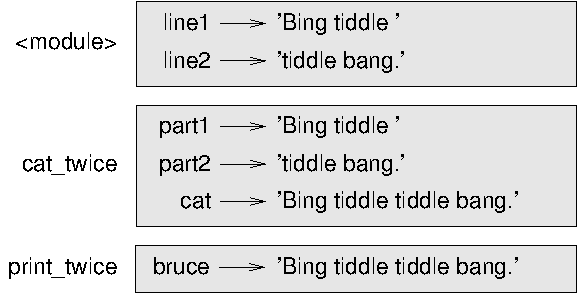
\includegraphics[scale=0.8]{figs/stack.pdf}}
\caption{Stack diagram.}
\label{fig.stack}
\end{figure}

\gr
Τα πλαίσια είναι διατεταγμένα σε μία στοίβα
η οποία υποδεικνύει ποια συνάρτηση καλεί ποια, και ούτω καθεξής. Σε αυτό το
παράδειγμα, η \en \verb"print_twice" \gr καλείται από την \en \verb"cat_twice"
\gr και η \en \verb"cat_twice" \gr έχει καλεστεί από την \en \verb"__main__",\gr
η οποία είναι η συνάρτηση για το ανώτατο πλαίσιο. Όταν δημιουργείτε μία
μεταβλητή έξω από οποιαδήποτε συνάρτηση, ανήκει στην \en \verb"__main__".

\gr
Κάθε παράμετρος αναφέρεται στην τιμή του αντίστοιχου ορίσματός της.
Έτσι, η \en {\tt part1} \gr έχει την ίδια τιμή με την \en {\tt line1}, \gr
η \en {\tt part2} \gr έχει την ίδια τιμή με την \en {\tt line2} \gr και
η \en {\tt bruce} \gr έχει την ίδια τιμή με την \en {\tt cat}.

\gr
Αν παρουσιαστεί ένα λάθος κατά την κλήση μιας συνάρτησης, η \en Python
\gr εμφανίζει το όνομα της συνάρτησης, το όνομα της συνάρτησης που την κάλεσε
και το όνομα της συνάρτησης η οποία κάλεσε αυτήν, \gr μέχρις ότου φτάσει στην
\en  \verb"__main__".


\gr
Για παράδειγμα, αν προσπαθήσετε να χρησιμοποιήσετε την \en {\tt cat} \gr
μέσα στην \en \verb"print_twice", \gr παίρνετε ένα μήνυμα λάθους \en {\tt NameError}:


\begin{verbatim}
Traceback (innermost last):
  File "test.py", line 13, in __main__
    cat_twice(line1, line2)
  File "test.py", line 5, in cat_twice
    print_twice(cat)
  File "test.py", line 9, in print_twice
    print cat
NameError: name 'cat' is not defined
\end{verbatim}
%
\gr
Αυτή η λίστα συναρτήσεων ονομάζεται αναδρομή προς τα πίσω. Σας πληροφορεί σε
ποιο φάκελο του προγράμματος παρουσιάστηκε το λάθος, σε ποια γραμμή και ποιες
συναρτήσεις εκτελούνταν εκείνη τη στιγμή. Σας δείχνει επίσης, τη γραμμή του κώδικα
από την οποία προκλήθηκε το λάθος.
\index{traceback}

Η σειρά των συναρτήσεων στην αναδρομή είναι ίδια με την σειρά των
πλαισίων στο στατικό διάγραμμα. Η συνάρτηση η οποία τρέχει αυτή τη στιγμή,
βρίσκεται στο κάτω μέρος.



\section{Γόνιμες και κενές συναρτήσεις}
\index{fruitful function}
\index{void function}
\index{function, fruitful}
\index{function, void}

Κάποιες από τις συναρτήσεις που χρησιμοποιούμε, όπως οι συναρτήσεις
μαθηματικών επιστρέφουν αποτελέσματα. Λόγω έλλειψης κάποιου καλύτερου ονόματος, τις
ονομάζω γόνιμες συναρτήσεις. 'Αλλες συναρτήσεις, όπως η \en \verb"print_twice",
\gr εκτελούν μια ενέργεια αλλά δεν επιστρέφουν τιμή. Αυτές ονομάζονται κενές \en (void)
\gr συναρτήσεις.

Όταν καλείτε μία γόνιμη συνάρτηση, σχεδόν πάντα θέλετε να χρησιμοποιήσετε
το αποτέλεσμα της. Για παράδειγμα, ίσως το εκχωρήσετε σε μία μεταβλητή ή να το
χρησιμοποιήσετε ως μέρος μιας έκφρασης \en : \gr

\en
\begin{verbatim}
x = math.cos(radians)
golden = (math.sqrt(5) + 1) / 2
\end{verbatim}
%
\gr
Όταν καλείτε μια συνάρτηση σε διαδραστική λειτουργία, η \en Python \gr
εμφανίζει το αποτέλεσμα:

\en
\begin{verbatim}
>>> math.sqrt(5)
2.2360679774997898
\end{verbatim}
%
\gr
Αλλά σε ένα σενάριο, αν καλέσετε μια γόνιμη συνάρτηση από μόνη της,
η επιστρεφόμενη τιμή έχει χαθεί για πάντα \en !


\begin{verbatim}
math.sqrt(5)
\end{verbatim}
%
\gr
Αυτό το σενάριο υπολογίζει την τετραγωνική ρίζα του 5, αλλά από την στιγμή που
δεν αποθηκεύει ή εμφανίζει το αποτέλεσμα, δεν είναι και πολύ χρήσιμο.
\index{interactive mode}
\index{script mode}

Οι κενές \en (void) \gr συναρτήσεις ίσως εμφανίσουν κάτι στην οθόνη ή έχουν κάποιο
αποτέλεσμα, αλλά δεν έχουν επιστρεφόμενη τιμή. Αν προσπαθήσετε να εκχωρήσετε το
αποτέλεσμα σε μία μεταβητή, θα πάρετε μια ειδική τιμή την ονομαζόμενη \en {\tt None}.
\index{None special value}
\index{special value!None}

\begin{verbatim}
>>> result = print_twice('Bing')
Bing
Bing
>>> print result
None
\end{verbatim}
%
\gr
Η τιμή \en {\tt None} \gr δεν είναι ίδια με την συμβολοσειρά \en \verb"'None'".
\gr Είναι μια ειδική τιμή η οποία έχει τον δικό της τύπο:

\en
\begin{verbatim}
>>> print type(None)
<type 'NoneType'>
\end{verbatim}
%
\gr
Μέχρι στιγμής, οι συναρτήσεις οι οποίες έχουμε γράψει είναι όλες κενές \en (void). \gr
Θα ξεκινήσουμε να γράφουμε γόνιμες συναρτήσεις σε μερικά κεφάλαια.


\section{Γιατί συναρτήσεις}
\index{function, reasons for}

Ίσως να μην είναι σαφές ο λόγος για τον οποίο αξίζει να χωρίζουμε
ένα πρόγραμμα σε συναρτήσεις. Υπάρχουν αρκετοί λόγοι:


\begin{itemize}

\item Η δημιουργία μιας νέας συνάρτησης σας δίνει την δυνατότητα να ονομάσεις
ένα σύνολο δηλώσεων, κάτι που κάνει το πρόγραμμα ευκολότερο στην ανάγνωση
και στην αποσφαλμάτωση.


\item Οι συναρτήσεις μπορούν να κάνουν ένα πρόγραμμα μικρότερο καταργώντας
τον επαναλαμβανόμενο κώδικα. Αν κάνετε κάποια αλλαγή αργότερα, θα χρειαστεί
να την κάνετε μόνο σε ένα σημείο.


\item Η διαίρεση ενός μεγάλου προγράμματος σε συναρτήσεις σας επιτρέπει να
αποσφαλματώσετε τα κομμάτια ένα τη φορά και μετά να τα συναθροίσετε
σε ένα ολόκληρο λειτουργικό πρόγραμμα.


\item Οι καλοσχεδιασμένες συναρτήσεις είναι συχνά χρήσιμες για πολλά προγράμματα.
Μόλις γράψετε μία και την αποσφαλματώσετε, μπορείτε να την χρησιμοποιήσετε πολλές φορές.


\end{itemize}

\gr
\section{Εισαγωγή από μονάδα λογισμικού}

Η \en Python \gr παρέχει δύο τρόπους εισαγωγής μονάδων λογισμικού.
Έχουμε ήδη δει έναν:

\en
\begin{verbatim}
>>> import math
>>> print math
<module 'math' (built-in)>
>>> print math.pi
3.14159265359
\end{verbatim}
%
\gr
Αν εισάγετε την \en {\tt math}, \gr θα πάρετε ένα αντικείμενο μονάδας λογισμικού με όνομα
\en  {\tt math}. \gr Το αντικείμενο αυτό περιέχει σταθερές όπως η \en {\tt pi} \gr
και συναρτήσεις όπως η \en {\tt sin} \gr και η \en {\tt exp}.

\gr
Αλλά αν προσπαθήσετε να αποκτήσετε απευθείας πρόσβαση στην \en {\tt pi}, \gr
θα πάρετε ένα μήνυμα λάθους.

\en
\begin{verbatim}
>>> print pi
Traceback (most recent call last):
  File "<stdin>", line 1, in <module>
NameError: name 'pi' is not defined
\end{verbatim}
%
\gr
Εναλλακτικά, μπορείτε να εισάγετε ένα αντικείμενο από μια μονάδα έτσι:

\en
\begin{verbatim}
>>> from math import pi
\end{verbatim}
%
\gr
Τώρα μπορείτε να έχετε απευθείας πρόσβαση στην \en {\tt pi}, \gr χωρίς
τον συμβολισμό τελείας.
\index{dot notation}

\en
\begin{verbatim}
>>> print pi
3.14159265359
\end{verbatim}
%
\gr
Ή μπορείτε να χρησιμοποιήσετε τον τελεστή αστερίσκου για να τα εισάγετε
 όλα από την μονάδα:

\en
\begin{verbatim}
>>> from math import *
>>> cos(pi)
-1.0
\end{verbatim}

\gr
Το πλεονέκτημα του να εισάγουμε τα πάντα από τη μαθηματική μονάδα λογισμικού είναι ότι μπορεί
ο κώδικάς σας να είναι πιο συνοπτικός. Το μειονέκτημα είναι ότι μπορεί ενδεχομένως,
να υπάρξουν αντιφάσεις στα ονόματα που έχουν οριστεί σε διαφορετικές μονάδες, ή μεταξύ ενός
ονόματος από μία μονάδα και μίας από τις μεταβλητές σας.



\section{Αποσφαλμάτωση}
\label{editor}
\index{debugging}

Αν χρησιμοποιείτε έναν επεξεργαστή κειμένου για να γράψετε τα σενάριά σας,
ίσως αντιμετωπίσετε προβλήματα με τα κενά διαστήματα και τις εσοχές κειμένου \en (tabs).
\gr Ο καλύτερος τρόπος για να αποφύγετε τέτοιου είδους προβλήματα είναι να χρησιμοποιείτε
αποκλειστικά κενά διαστήματα (όχι εσοχές\en (tabs)). \gr Οι περισσότεροι κειμενογράφοι που γνωρίζουν
\en Python \gr το κάνουν αυτό εξ ορισμού, αλλά κάποιοι άλλοι δεν το κάνουν.
\index{whitespace}

Συνήθως, οι εσοχές και τα κενά διαστήματα είναι αόρατα, κάτι το οποίο
δυσκολεύει την αποσφαλμάτωση, γι αυτό προσπαθήστε να βρείτε έναν επεξεργαστή
που θα διαχειριστεί την ενδοπαραγραφοποίηση για εσάς.

Επίσης, μην ξεχνάτε να αποθηκεύετε το πρόγραμμά σας προτού το τρέξετε.
Κάποια περιββάλοντα ανάπτυξης το κάνουν αυτόματα, αλλά κάποια άλλα όχι.
Σε αυτήν την περίπτωση, το πρόγραμμα που κοιτάτε στον επεξεργαστή δεν είναι
το ίδιο με το πρόγραμμα που τρέχετε.

Η αποσφαλμάτωση μπορεί να είναι χρονοβόρα αν τρέχετε συνεχώς το ίδιο,
εσφαλμένο πρόγραμμα ξανά και ξανά!

Σιγουρευτείτε πως ο κώδικας που κοιτάτε είναι ο κώδικας που τρέχετε.
Αν δεν είστε σίγουροι, γράψτε κάτι όπως η \en \verb"print 'hello'" \gr
στην αρχή του προγράμματός σας και τρέξτε το ξανά. Αν δεν δείτε την \en
\verb"hello", \gr δεν τρέχετε το σωστό πρόγραμμα!



3.15
\section{Ορολογία}

\begin{description}

\item[συνάρτηση:] Μία ακολουθία δηλώσεων με συγκεκριμένη ονομασία η οποία εκτελεί κάποιες
χρήσιμες λειτουργίες. Οι συναρτήσεις μπορούν ή δεν μπορουν να λάβουν ορίσματα
και μπορούν ή όχι να παράγουν ένα αποτέλεσμα.
\index{function}

\item[ορισμός συνάρτησης:] Είναι μία δήλωση η οποία δημιουργεί μια νέα συνάρτηση,
συγκεκριμενοποιώντας το όνομα της, τις παραμέτρους και τις δηλώσεις που εκτελεί.
\index{function definition}

\item[αντικείμενο συνάρτησης: ] Μία τιμή η οποία δημιουργείται από τον ορισμό μιας συνάρτησης.
Το όνομα της συνάρτησης είναι μία μεταβλητή η οποία αναφέρεται σε ένα αντικείμενο
συνάρτησης.
\index{function definition}

\item[επικεφαλίδα:] Η πρώτη γραμμή του ορισμού μιας συνάρτησης.
\index{header}

\item[σώμα:] Η ακολουθία δηλώσεων μέσα σε έναν ορισμό συνάρτησης.
\index{body}

\item[παράμετρος:] Ένα όνομα το οποίο χρησιμοποιείται μέσα σε μία συνάρτηση για να
αναφερθεί στη τιμή που περνιέται σαν όρισμα.
\index{parameter}

\item[κλήση συνάρτησης:] Μία δήλωση η οποία εκτελεί μια συνάρτηση. Αποτελείται από το
όνομα της συνάρτησης ακολουθούμενο από μία λίστα ορισμάτων.
\index{function call}

\item[όρισμα:] Μία τιμή η οποία παρέχεται σε μια συνάρτηση όταν αυτή καλείται.
Αυτή η τιμή εκχωρείται στην αντίστοιχη παράμετρο στη συνάρτηση.
\index{argument}

\item[τοπική μεταβλητή:] Μία μεταβλητή οριζόμενη μέσα σε μια συνάρτηση. Μια τοπική
μεταβλητή μπορεί να χρησιμοποιείται μόνο μέσα στη συνάρτησή της.
\index{local variable}

\item[επιστρεφόμενη τιμή:] Το αποτέλεσμα μιας συνάρτησης. Αν μια κλήση συνάρτησης
χρησιμοποιείται σαν μια έκφραση, η επιστρεφόμενη τιμή είναι η τιμή της έκφρασης.
\index{return value}

\item[γόνιμη συνάρτηση:] Μία συνάρτηση η οποία επιστρέφει μια τιμή.
\index{fruitful function}

\item[κενή \en (void) \gr συνάρτηση:] Μία συνάρτηση η οποία δεν επιστρέφει κάποια τιμη.
\index{void function}

\item[μονάδα λογισμικου\en (module)\gr :] Ένας φάκελος ο οποίος περιέχει μία συλλογή
σχετικών συναρτήσεων και άλλους ορισμούς.
\index{module}

\item[δήλωση εισαγωγής:] Μία δήλωση η οποία διαβάζει μια μονάδα λογισμικού και δημιουργεί
ένα αντικείμενο μονάδας.
\index{import statement}
\index{statement!import}

\item[αντικείμενο μονάδας λογισμικού:] Μία τιμή που δημιουργείται από την δήλωση \en  {\tt import} \gr
και παρέχει πρόσβαση στις τιμές που ορίστηκαν μέσα σε μία μονάδα λογισμικού.
\index{module}

\item[συμβολισμός με τελεία:] Η σύνταξη για να καλείτε μια συνάρτηση σε μια άλλη μονάδα λογισμικού
προσδιορίζοντας το όνομα της μονάδας ακολουθούμενο από μία τελεία και το όνομα της συνάρτησης.
\index{dot notation}

\item[σύνθεση:] Η χρήση μιας έκφρασης ως μέρος μιας μεγαλύτερης έκφρασης,
ή μιας δήλωσης ως μέρος μιας μεγαλύτερης δήλωσης.
\index{composition}

\item[ροή εκτέλεσης:] Η σειρά με την οποία εκτελούνται οι δηλώσεις κατά το τρέξιμο του προγράμματος.
\index{flow of execution}

\item[διάγραμμα στοίβας:] Μία γραφική αναπαράσταση μιας στοίβας συναρτήσεων,
των μεταβλητών τους και των τιμών στις οποίες αναφέρονται.
\index{stack diagram}

\item[πλαίσιο:] Ένα κουτί σε ένα διάγραμμα στοίβας το οποίο αναπαριστά μια κλήση συνάρτησης.
Περιέχει τις τοπικές μεταβλητές και τις παραμέτρους της συνάρτησης.
\index{function frame}
\index{frame}

\item[αναδρομή:] Μία λίστα των συναρτήσεων που εκτελούνται, τυπώνεται όταν παρουσιαστεί
μια εξαίρεση.
\index{traceback}


\end{description}


\section{Ασκήσεις}

ΑΣΚΗΣΗ 3.3
\index{len function}
\index{function!len}

Η \en Python \gr έχει ενσωματωμένες συναρτήσεις, οι οποίες ονομάζονται \en {\tt len} \gr και
οι οποίες επιστρέφουν το μήκος μιας συμβολοσειράς, έτσι ώστε η τιμή της \en \verb"len('allen')"
\gr να είναι 5.

Γράψτε μία συνάρτηση με όνομα \en \verb"right_justify" \gr η οποία παίρνει
μία συμβολοσειρά με όνομα \en {\tt s} \gr σαν μία παράμετρο και να
εκτυπώνει την συμβολοσειρά με αρκετά κενά διαστήματα έτσι ώστε το τελευταίο γράμμα της
συμβολοσειράς να είναι στη στήλη 70 της οθόνης.

\en
\begin{verbatim}
>>> right_justify('allen')
                                                                 allen
\end{verbatim}

\gr
ΑΣΚΗΣΗ 3.4
\index{function object}
\index{object!function}

Ένα αντικείμενο συνάρτησης είναι μια τιμή την οποία, μπορείτε να εκχωρήσετε
σε μία μεταβλητή ή να την περάσετε σαν ένα όρισμα. Για παράδειγμα, η \en \verb"do_twice"
\gr είναι μία συνάρτηση η οπόια παίρνει ένα αντικείμενο συνάρτησης σαν ένα όρισμα και το καλεί δύο φορές:

\en
\begin{verbatim}
def do_twice(f):
    f()
    f()
\end{verbatim}
\gr
Ένα παράδειγμα το οποίο χρησιμοποιεί την \en  \verb"do_twice" \gr  για να καλέσει
μία συνάρτηση που ονομάζεται \en \verb"print_spam" \gr δύο φορές είναι:

\en
\begin{verbatim}
def print_spam():
    print 'spam'

do_twice(print_spam)
\end{verbatim}

\begin{enumerate}

\gr
\item Πληκτρολογήστε  αυτό το παράδειγμα σε ένα σενάριο και ελέγξτε το.


\item Τροποποιήστε την \en  \verb"do_twice" \gr έτσι ώστε να δέχεται δύο ορίσματα, ένα
αντικείμενο συνάρτησης και μία τιμή και να καλεί την συνάρτηση δύο φορές, περνώντας την τιμή σαν όρισμα.


\item Γράψτε μία γενικότερη εκδοχή της \en \verb"print_spam", \gr με όνομα
\en \verb"print_twice",  \gr η οποία παίρνει μια συμβολοσειρά σαν παράμετρο και την
εκτυπώνει δύο φορές.


\item Χρησιμοποιήστε την τροποποιημένη εκδοχή της \en  \verb"do_twice" \gr για να καλέσετε
την \en \verb"print_twice" \gr δύο φορές, περνώντας την \en \verb"'spam'" \gr σαν όρισμα.


\item Προσδιορίστε μία νέα συνάρτηση ονομαζόμενη \en \verb"do_four" \gr η οποία
παίρνει ένα αντικείμενο συνάρτησης και μία τιμή και καλεί την συνάρτηση τέσσερις φορές, περνώντας
την τιμή σαν μία παράμετρο. Πρέπει να ύπαρχουν μόνο δύο δηλώσεις στο σώμα συτής της
συνάρτησης, όχι τέσσερις.


\end{enumerate}
\gr
Λύση: \en \url{http://thinkpython.com/code/do_four.py}.

\gr


ΑΣΚΗΣΗ 3.5

Αυτή η άσκηση μπορεί να υλοποιηθεί με τη χρήση δηλώσεων και άλλων
χαρακτηριστικών που έχουμε μάθει μέχρι στιγμής.


\begin{enumerate}

\item Γράψτε μία συνάρτηση η οποία σχεδιάζει ένα πλέγμα όπως το ακόλουθο\en :
\index{grid}


\begin{verbatim}
+ - - - - + - - - - +
|         |         |
|         |         |
|         |         |
|         |         |
+ - - - - + - - - - +
|         |         |
|         |         |
|         |         |
|         |         |
+ - - - - + - - - - +
\end{verbatim}
%
\gr
Σημείωση: Για να εμφανίσετε περισσότερες απο μία τιμές σε μία γραμμή, μπορείτε να εμφανίσετε
μία ακολουθία χωρισμένη με κόμματα:

\en
\begin{verbatim}
print '+', '-'
\end{verbatim}
%
\gr
Αν η ακολουθία τελειώνει με κόμμα, η \en Python \gr αφήνει την γραμμή ημιτελή,
έτσι ώστε η επόμενη εμφανιζόμενη τιμή να εμφανιστεί στην ίδια γραμμή.

\en
\begin{verbatim}
print '+',
print '-'
\end{verbatim}
%
\gr
Η έξοδος αυτών των δηλώσεων είναι \en \verb"'+ -'". \gr

Μία δήλωση \en {\tt print} \gr από μόνη της ολοκληρώνει την τρέχουσα γραμμή
και πηγαίνει στην επόμενη γραμμή.

\item Γράψτε μία συνάρτηση η οποία σχεδιάζει ένα παρόμοιο πλέγμα
με τέσσερις σειρές και τέσσερις στήλες.


\end{enumerate}
\gr
Λύση: \en \url{http://thinkpython.com/code/grid.py}. \gr
Αυτή η άσκηση είναι βασισμένη σε μία άσκηση του \en Oualline,
{\em Practical C Programming, Third Edition}, O'Reilly Media, 1997.

\gr




\chapter{Μελέτη περίπτωσης: σχεδίαση διεπαφής}
\label{turtlechap}

Τα παραδείγματα κώδικα αυτού του κεφαλαίου είναι διαθέσιμα στην διεύθυνση \en
\url{http://thinkpython.com/code/polygon.py}.


\section{TurtleWorld}
\label{turtleworld}
\index{TurtleWorld}
\index{Swampy}
\gr
Για να συνοδεύσω αυτό το βιβλίο, έχω γράψει ένα πακέτο λογισμικού που λέγεται
\en Swampy. \gr Μπορείτε να κατεβάσετε το \en Swampy \gr από τον σύνδεσμο
\en  \url{http://thinkpython.com/swampy} \gr και ακολουθήστε τις οδηγίες εκεί για να
εγκαταστήσετε το \en  Swampy \gr στον υπολογιστή σας.

Ένα πακέτο λογισμικού είναι μια συλλογή μονάδων λογισμικού. Μία από τις μονάδες του \en Swampy
\gr είναι η \en {\tt TurtleWorld} \gr η οποία παρέχει ένα σύνολο συναρτήσεων για τον
σχεδιασμό γραμμών κατευθύνοντας χελώνες στην οθόνη.
\index{package}

Αν το \en Swampy \gr έχει εγκατασταθεί σαν ένα πακέτο λογισμικού στον υπολογιστή σας,
μπορείτε να εισάγετε την \en {\tt TurtleWorld} \gr με τον εξής τροπο:

\en
\begin{verbatim}
from swampy.TurtleWorld import *
\end{verbatim}

\gr
Αν κατεβάσατε τις μονάδες του \en Swampy \gr αλλά δεν τις εγκαταστήσατε σαν πακέτο,
μπορείτε είτε να δουλέψετε στον κατάλογο ο οποίος περιέχει τα αρχεία του \en Swampy \gr
είτε να προσθέσετε αυτόν τον κατάλογο στην διαδρομή αναζήτησης της \en Python. \gr Τότε
μπορείτε να εισάγετε την \en {\tt TurtleWorld} \gr έτσι:

\en
\begin{verbatim}
from TurtleWorld import *
\end{verbatim}

\gr
Οι λεπτομέρειες της διαδικασίας εγκατάστασης και της προσθήκης της διαδρομής
αναζήτησης στην \en Python \gr εξαρτώνται από τον υπολογιστή σας, έτσι αντί να
συμπεριλάβω αυτές τις λεπτομέρειες εδώ, θα προσπαθήσω να διατηρήσω τις παρούσες
πληροφορίες για διάφορα συστήματα στην διεύθυνση \en \url{http://thinkpython.com/swampy}.

\gr
Δημιουργήστε ένα φάκελο με το όνομα \en {\tt mypolygon.py} \gr και πληκτρολογήστε
τον ακόλουθο κώδικα:

\en
\begin{verbatim}
from swampy.TurtleWorld import *

world = TurtleWorld()
bob = Turtle()
print bob

wait_for_user()
\end{verbatim}
%
\gr
Η πρώτη γραμμή εισάγει ό,τι υπάρχει στην μονάδα \en {\tt TurtleWorld} \gr
του πακέτου \en {\tt swampy}. \gr
\index{import statement}
\index{statement!import}

Οι επόμενες γραμμές δημιουργούν την \en TurtleWorld \gr η οποία εκχωρείται στην
\en {\tt world} \gr και μία \en Turtle \gr η οποία εκχωρείται στην \en {\tt bob}. \gr
Εκτυπώνοντας την \en {\tt bob} \gr παράγεται κάτι όπως:

\en
\begin{verbatim}
<TurtleWorld.Turtle instance at 0xb7bfbf4c>
\end{verbatim}
%
\gr
Αυτό σημαίνει ότι η \en {\tt bob} \gr αναφέρεται σε ένα στιγμιότυπο της \en Turtle \gr
όπως ορίζεται στην μονάδα της \en {\tt TurtleWorld}. \gr Σε αυτό το πλαίσιο, το \en "\gr στιγμιότυπο\en " \gr
\en (''instance'')  \gr σημαίνει ένα τμήμα ενός συνόλου. Αυτή η \en Turtle  \gr είναι μία από
το σύνολο των εφικτών \en Turtles.
\index{instance}

H \en \verb"wait_for_user" \gr λέει στην \en TurtleWorld \gr
να περιμένει από τον χρήστη να κάνει κάτι, παρόλο που σε αυτήν
τη περίπτωση δεν υπάρχουν και πολλά που μπορεί να κάνει ο χρήστης
εκτός από το να κλείσει το παράθυρο.

Η \en TurtleWorld  \gr παρέχει αρκετές \en "\gr χελωνο-κατευθυνόμενες\en " \gr
συναρτήσεις: την \en  {\tt fd} \gr και την \en {\tt bk} \gr για μπροστά και πίσω,
την \en {\tt lt} \gr και την \en {\tt rt} \gr για στροφή στα αριστερά και στα δεξιά.
Η κάθε χελώνα επίσης, κρατάει ένα στιλό, ο οποίος βρίσκεται είτε κάτω είτε πάνω.
Αν το στιλό βρίσκεται κάτω, η χελώνα αφήνει μια γραμμή όταν κινείται. Οι συναρτήσεις
\en {\tt pu} \gr και \en  {\tt pd} \gr αντιπροσωπεύουν τα \en ``pen up'' \gr και \en ``pen down.''
\gr

Για να σχεδιάσετε μια ορθή γωνία, προσθέστε αυτές τις γραμμές στο πρόγραμμα
(αφού δημιουργήσετε την \en {\tt bob} \gr και προτού καλέσετε την \en \verb"wait_for_user"):

\begin{verbatim}
fd(bob, 100)
lt(bob)
fd(bob, 100)
\end{verbatim}
%
\gr
Η πρώτη γραμμή λέει στην \en {\tt bob} \gr να κάνει 100 βήματα μπροστά.
Η δεύτερη γραμμή του λέει να στρίψει αριστερά.

Όταν τρέχετε αυτό το πρόγραμμα, θα πρέπει να δείτε την \en {\tt bob} \gr να
μετακινείται ανατολικά και μετά βόρεια, αφήνοντας δύο ευθύγραμμα τμήματα πίσω.

Τροποποιήστε το πρόγραμμα για να σχεδιάσετε ένα τετράγωνο. Μη προχωρήσετε μέχρι
να αρχίσει να δουλεύει.

%\newpage

\section{Απλή επανάληψη}
\label{repetition}
\index{repetition}


Σκεφτείτε να γράφατε κάτι τέτοιο (χωρίς τον κώδικα ο οποίος δημιουργεί
την \en TurtleWorld \gr και περιμένει τον χρήστη) \en :

\begin{verbatim}
fd(bob, 100)
lt(bob)

fd(bob, 100)
lt(bob)

fd(bob, 100)
lt(bob)

fd(bob, 100)
\end{verbatim}
%
\gr
Μπορούμε να κάνουμε την ίδια διαδικασία πιο συνοπτικά με μία δήλωση \en {\tt for}. \gr
Προσθέστε αυτό το παράδειγμα στην \en {\tt mypolygon.py} \gr και τρέξτε το ξανά:
\index{for loop}
\index{loop!for}
\index{statement!for}

\en
\begin{verbatim}
for i in range(4):
    print 'Hello!'
\end{verbatim}
%
\gr
Θα πρέπει να δείτε κάτι τέτοιο:

\en
\begin{verbatim}
Hello!
Hello!
Hello!
Hello!
\end{verbatim}
%
\gr
Αυτή είναι η πιο απλουστευμένη χρήση της δήλωσης \en {\tt for}. \gr Θα δούμε περισσότερες χρήσεις
αργότερα. Αλλά αυτό είναι αρκετό ώστε να μπορείτε να ξαναγράψετε το πρόγραμμα σχεδιασμού τετραγώνων.
Μην προχωρήσετε μέχρι να το κάνετε.

Μία δήλωση \en {\tt for} \gr που σχεδιάζει τετράγωνα είναι \en :

\begin{verbatim}
for i in range(4):
    fd(bob, 100)
    lt(bob)
\end{verbatim}
%
\gr
Η σύνταξη μίας δήλωσης \en {\tt for} \gr είναι παρόμοια με τον ορισμό μιας
συνάρτησης. Έχει μία επικεφαλίδα που τελειώνει με μία άνω και κάτω τελεία και ένα
σώμα εμφωλευμένο. Το σώμα δεν έχει συγκεκριμένο αριθμό δηλώσεων.
\index{loop}

Μία δήλωση \en {\tt for} \gr μερικές φορές ονομάζεται \en {\bf loop} \gr επειδή
η ροή εκτέλεσης περνά μέσα από το σώμα και στη συνέχεια επιστρέφει βρογχοειδώς
πίσω στην κορυφή. Σε αυτή την περίπτωση, τρέχει το σώμα τέσσερις φορές.

Αυτή η εκδοχή είναι στην πραγματικότητα λίγο διαφορετική από τον προηγούμενο
κώδικα σχεδίασης τετραγώνων δεδομένου ότι κάνει ακόμη μία στροφή αφότου σχεδιάσει την τελευταία
πλευρά του τετραγώνου. Η επιπλέον στροφή παίρει λίγο περισσότερο χρόνο, αλλά απλοποιεί τον κώδικα αν κάνουμε
το ίδιο πράγμα κάθε φορά μέσα στο βρόγχο. Αυτή η εκδοχή έχει επίσης ως αποτέλεσμα να αφήνει τη χελώνα
στην αρχική θέση, με φορά προς την αρχική κατεύθυνση.


\section{Ασκήσεις}

Τα παρακάτω είναι μία σειρά ασκήσεων οι οποίες χρησιμοποιούν τη \en TurtleWorld. \gr
Προορίζονται για διασκέδαση, αλλά έχουν και κάποιο νόημα. Ενώ εργάζεστε σε αυτές, σκεφτείτε
ποιο είναι το νόημα.

Οι παρακάτω ενότητες έχουν λύσεις στις ασκήσεις, γι αυτό μην τις κοιτάξετε μέχρι να τις λύσετε
(ή τουλάχιστον προσπαθήστε).

\begin{enumerate}

\item Γράψτε μία συνάρτηση με το όνομα \en {\tt square} \gr που θα παίρνει μια παράμετρο με το όνομα
\en {\tt t}, \gr η οποία είναι μία χελώνα. Θα πρέπει να χρησιμοποιήσει τη χελώνα για να σχεδιάσει
ένα τετράγωνο.

Γράψτε μία κλήση συνάρτησης η οποία περνάει την \en {\tt bob} \gr
σαν ένα όρισμα στην \en {\tt square}, \gr έπειτα ξανατρέξτε το πρόγραμμα.

\item Προσθέστε μία άλλη παράμετρο με όνομα \en {\tt length}, \gr στη \en {\tt square}. \gr
Τροποποιήστε το σώμα ώστε το μήκος των πλευρών να είναι η \en {\tt length}, \gr μετά
τροποποιήστε την κλήση της συνάρτησης για να δώσετε ένα δεύτερο όρισμα. Τρέξτε το πρόγραμμα ξανά.
Ελέγξτε το πρόγραμμά σας για διάφορες τιμές για την \en  {\tt length}. \gr

\item Οι συναρτήσεις \en {\tt lt} \gr και \en {\tt rt} \gr κάνουν στροφές 90 μοιρών
από προεπιλογή, αλλά μπορείτε να δώσετε ένα δεύτερο όρισμα που να
καθορίζει τον αριθμό των μοιρών. Για παράδειγμα, η  \en {\tt lt(bob, 45)} \gr στρέφει τη \en {\tt lt(bob, 45)}
45 \gr μοίρες στα αριστερά.

Κάντε ένα αντίγραφο της \en {\tt square} \gr και αλλάξτε το όνομά της σε
\en {\tt polygon}. \gr Προσθέστε μία παράμετρο με όνομα \en {\tt n} \gr και
τροποποιήστε το σώμα ώστε να σχεδιάζει ένα κανονικό πολύγωνο \en n \gr πλευρών.
Σημείωση: Οι εξωτερικές γωνίες ενός κανονικού πολυγώνου \en n \gr πλευρών είναι
$360/n$ μοίρες.
\index{polygon function}
\index{function!polygon}

\item Γράψτε μία συνάρτηση με όνομα \en {\tt circle} \gr η οποία παίρνει μία χελώνα \en {\tt t}, \gr
και τα ακτίνια \en {\tt r} \gr ως παράμετρους και σχεδιάζει έναν κατά προσέγγιση κύκλο επικαλούμενη τη \en
{\tt polygon} \gr με ένα κατάλληλο μήκος και αριθμό πλευρών. Ελέγξτε τη συνάρτησή σας με ένα εύρος τιμών της
\en {\tt r}.
\index{circle function}
\index{function!circle}
\gr
Σημείωση 1η: Υπολογίστε την περίμετρο του κύκλου και σιγουρευτείτε πως \en {\tt length * n = \gr περίμετρος\en}.
\gr
Σημείωση 2η: Αν η \en {\tt bob} \gr είναι πολύ αργή για σας, μπορείτε να την επιταχύνετε αλλάζοντας
την \en {\tt bob.delay}, \gr η οποία είναι ο χρόνος μεταξύ των κινήσεων, σε δευτερόλεπτα. H \en {\tt bob.delay = 0.01} \gr θα πρέπει να τον κάνει να κινείται γρηγορότερα.

% Αλλάξτε το σε \en world.delay
% change this to world.delay

\item Φτιάξτε μία πιο γενική έκδοση της \en {\tt circle} \gr με όνομα \en {\tt arc} \gr
η οποία παίρνει μία επιπλέον παράμετρο την \en {\tt angle}, \gr η οποία καθορίζει ποιο τμήμα ενός κύκλου
θα σχεδιαστεί. Η \en {\tt angle} \gr μετρείται σε μοίρες, έτσι όταν η \en{\tt angle=360} \gr η \en {\tt arc}
\gr θα πρέπει να σχεδιάσει ένα πλήρες κύκλο.
\index{ function}
\index{function!arc}

\end{enumerate}

\section{Ενθυλάκωση}

Η πρώτη άσκηση σας ζητάει να βάλετε τον κώδικα σχεδίασης τετραγώνων σε
έναν ορισμό συνάρτησης και μετά να καλέσετε τη συνάρτηση, περνώντας τη χελώνα σαν μία
παράμετρο. Αυτή είναι μία λύση:

\en
\begin{verbatim}
def square(t):
    for i in range(4):
        fd(t, 100)
        lt(t)

square(bob)
\end{verbatim}
%
\gr
Οι ενδότερες δηλώσεις \en {\tt fd} \gr και \en {\tt lt} \gr είναι διπλά εμφωλευμένες για να
δείξουν ότι βρίσκονται εντός του βρόγχου \en {\tt for}, \gr ο οποίος βρίσκεται μέσα στον
ορισμό της συνάρτησης. Η επόμενη γραμμή, \en {\tt square(bob)}, \gr βρίσκεται στο
ίδιο επίπεδο με το αριστερό όριο, ώστε να είναι το τέλος του βρόγχου \en {\tt for} \gr και του
ορισμού της συνάρτησης.

Μέσα στη συνάρτηση, η \en {\tt t} \gr αναφέρεται στην ίδια χελώνα που αναφέρεται και η
\en {\tt bob} \gr έτσι, η \en {\tt lt(t)} \gr έχει το ίδιο αποτέλεσμα με τη \en {\tt lt(bob)}. \gr
Οπότε γιατί να μην καλέσουμε την παράμετρο \en {\tt bob} ; \gr Η γενική ιδέα είναι ότι η \en {\tt t}
\gr μπορεί να είναι οποιαδήποτε χελώνα, όχι μόνο η \en {\tt bob}, \gr έτσι μπορείτε να δημιουργήσετε
μία δεύτερη χελώνα και να την περάσετε ως όρισμα στη \en {\tt square}:

\en
\begin{verbatim}
ray = Turtle()
square(ray)
\end{verbatim}
%
\gr
Το να συμπεριλάβετε ένα κομμάτι του κώδικα στη συνάρτηση ονομάζεται \en "\gr ενθυλάκωση\en ". \gr
Ένα από τα πλεονεκτήματα της ενθυλάκωσης είναι ότι προσδίδει ένα όνομα στον κώδικα, το οποίο
χρησιμεύει ως ένα είδος τεκμηρίωσης. Ένα άλλο πλεονέκτημα είναι πως αν χρησιμποποιήσετε ξανά τον
κώδικα, είναι πιο λακωνικό να καλέσετε δύο φορές μία συνάρτηση παρά να αντιγράφετε ολόκληρο το σώμα της\en !
\index{encapsulation}
\gr

\section{Γενίκευση}

Το επόμενο βήμα είναι να προσθέσουμε μία παράμετρο \en {\tt length} \gr στην \en {\tt square}.\gr
Αυτή είναι η λύση:

\en
\begin{verbatim}
def square(t, length):
    for i in range(4):
        fd(t, length)
        lt(t)

square(bob, 100)
\end{verbatim}
%
\gr
Η προσθήκη μίας παραμέτρου σε μία συνάρτηση ονομάζεται \en "\gr γενίκευση\en " \gr
διότι κάνει την συνάρτηση πιο γενική\en : \gr στην προηγούμενη εκδοχή, το τετράγωνο έχει πάντα το ίδιο
μέγεθος, ενώ σε αυτήν την εκδοχή μπορεί να έχει οποιοδήποτε μέγεθος.
\index{generalization}

Το επόμενο βήμα είναι επίσης μία γενίκευση. Αντί να σχεδιάζει τετράγωνα, η \en {\tt polygon} \gr
σχεδιάζει κανονικά πολύγωνα με οποιονδήποτε αριθμό πλευρών. Αυτή είναι η λύση:

\en
\begin{verbatim}
def polygon(t, n, length):
    angle = 360.0 / n
    for i in range(n):
        fd(t, length)
        lt(t, angle)

polygon(bob, 7, 70)
\end{verbatim}
%
\gr
Αυτό σχεδιάζει ένα πολύγωνο 7 πλευρών με μήκος πλευράς 70. Αν έχετε περισσότερα από μερικά
αριθμητικά ορίσματα, είναι εύκολο να ξεχάσετε τι είναι τι, ή σε ποια σειρά θα πρέπει να βρίσκονται.
Είναι έγκυρο, και κάποιες φορές χρήσιμο, να συμπεριλάβετε τα ονόματα των παραμέτρων στη λίστα ορισμάτων\en :

\begin{verbatim}
polygon(bob, n=7, length=70)
\end{verbatim}
%
\gr
Αυτά ονομάζονται \en "\gr λέξεις-κλειδιά ορίσματα\en " \gr επειδή περιέχουν τα ονόματα των παραμέτρων
ως \en "\gr λέξεις-κλειδιά\en " \gr (δεν θα πρέπει να συγχέονται με τις λέξεις κλειδιά της \en Python \gr
όπως είναι η \en {\tt while} \gr και η \en {\tt def}\gr ).
\index{keyword argument}
\index{argument!keyword}

Αυτή η σύνταξη κάνει το πρόγραμμα πιο ευανάγνωστο. Είναι επίσης μιά υπενθύμιση σχετικά με το πως
λειτουργούν τα ορίσματα και οι παράμετροι\en : \gr όταν καλείτε μία συνάρτηση τα ορίσματα εκχωρούνται στις
παραμέτρους.


\section{Σχεδίαση διεπαφής}

Το επόμενο βήμα είναι να γράψετε τη \en {\tt circle}, \gr η οποία παίρνει μία ακτίνα, την \en {\tt r},
\gr ως παράμετρο. Μία απλή λύση η οποία χρησιμοποιεί τη \en {\tt polygon} \gr για να σχεδιάσει ένα πολύγωνο
50 πλευρών\en :

\en
\begin{verbatim}
def circle(t, r):
    circumference = 2 * math.pi * r
    n = 50
    length = circumference / n
    polygon(t, n, length)
\end{verbatim}
%
\gr
Η πρώτη γραμμή υπολογίζει την περίμετρο ενός κύκλου με ακτίνα \en {\tt r} \gr
χρησιμοποιώντας τον τύπο \en $2 \pi r$. \gr Από τη στιγμή που χρησιμοποιούμε τη \en
{\tt math.pi}, \gr θα πρέπει να εισάγουμε τη \en {\tt math}. \gr Κατά συνθήκη, οι δηλώσεις
\en {\tt import} \gr είναι συνήθως στην αρχή του σεναρίου.

Η \en {\tt n} \gr είναι το πλήθος των ευθύγραμων τμημάτων στον κατά προσέγγιση κύκλο μας,
έτσι η \en {\tt length} \gr είναι το μήκος κάθε τμήματος. Επομένως, η \en {\tt polygon} \gr
σχεδιάζει ένα πολύγωνο 50 πλευρών το οποίο προσεγγίζει ένα κύκλο με ακτίνα \en {\tt r}. \gr

Ένας από τους περιορισμούς αυτής της λύσης είναι ότι η \en {\tt n} \gr είναι μία σταθερά,
το οποίο σημαίνει ότι για πολύ μεγάλους κύκλους, τα ευθύγραμμα τμήματα είναι πολύ μακριά, και
για μικρούς κύκλους, σπαταλάμε χρόνο σχεδιάζοντας πολύ μικρά τμήματα. Μία λύση θα ήταν να
γενικεύαμε τη συνάρτηση περνώντας την \en {\tt n} \gr σαν παράμετρο. Αυτό θα δώσει στο χρήστη
(όταν καλεί την \en {\tt circle}\gr ) περισσότερο έλεγχο, αλλά η διεπαφή θα γίνει λιγότερο
ξεκάθαρη.
\index{interface}

Η διεπαφή μίας συνάρτησης είναι μία σύνοψη του πως χρησιμοποιείται\en : \gr ποιες είναι
οι παράμετροι\en ; \gr τι κάνει η συνάρτηση\en ; \gr ποια είναι η επιστρεφόμενη τιμή\en ; \gr
Μία διεπαφή είναι \en "\gr ξεκάθαρη\en " \gr εάν είναι \en "\gr όσο το δυνατόν πιο απλή, αλλά όχι
απλούστερη. (Αϊνστάιν) \en "\gr
\index{Einstein, Albert}

Σε αυτό το παράδειγμα, η \en {\tt r} \gr ανήκει στη διεπαφή επειδή προσδιορίζει τον κύκλο που θα
σχεδιαστεί. Η \en {\tt n} \gr δεν είναι τόσο κατάλληλη επειδή αναφέρεται στις λεπτομέριες του πως
ο κύκλος θα πρέπει να καταστεί.

Αντί να υπερφορτώσουμε την διεπαφή, είναι καλύτερα να διαλέξουμε μία κατάλληλη
τιμή για την \en {\tt n} \gr ανάλογα με την περιφέρεια\en :

\begin{verbatim}
def circle(t, r):
    circumference = 2 * math.pi * r
    n = int(circumference / 3) + 1
    length = circumference / n
    polygon(t, n, length)
\end{verbatim}
%
\gr
Τώρα, ο αριθμός των τμημάτων είναι (περίπου) \en {\tt circumference/3}, \gr
έτσι το μήκος κάθε τμήματος είναι (περίπου) 3, το οποίο είναι αρκετά μικρό ώστε
ο κύκλος να φαίνεται καλός, αλλά και πολύ μεγάλο για να είναι αποδοτικό και κατάλληλο
για οποιοδήποτε μέγεθος κύκλου.


\section{Ανακατασκευή κώδικα}
\label{refactoring}
\index{refactoring}

Όταν έγραψα τη \en {\tt circle}, \gr είχα την δυνατότητα να επαναχρησιμοποιήσω τη \en {\tt polygon} \gr
επειδή ένα πολύπλευρο πολύγωνο είναι μία καλή προσέγγιση ενός κύκλου. Αλλά η \en {\tt arc} \gr δεν είναι
τόσο συνεργάσιμη. Δεν μπορούμε να χρησιμοποιήσουμε τη \en {\tt polygon} \gr ή τη \en {\tt circle} \gr για
να σχεδιάσουμε ένα τόξο.

Μία εναλλακτική λύση είναι να ξεκινήσουμε με ένα αντίγραφο της \en {\tt polygon} \gr και
να το μετατρέψουμε σε \en {\tt arc}. \gr Το αποτέλεσμα θα μπορούσε να είναι κάπως έτσι\en :

\begin{verbatim}
def arc(t, r, angle):
    arc_length = 2 * math.pi * r * angle / 360
    n = int(arc_length / 3) + 1
    step_length = arc_length / n
    step_angle = float(angle) / n

    for i in range(n):
        fd(t, step_length)
        lt(t, step_angle)
\end{verbatim}
%
\gr
Το δεύτερο μισό αυτής της συνάρτησης μοιάζει με τη \en {\tt polygon}, \gr αλλά
δεν μπορούμε να επαναχρησιμοποιήσουμε τη \en {\tt polygon} \gr χωρίς να αλλάξουμε τη
διεπαφή. Θα μπορούσαμε να γενικεύσουμε τη \en {\tt polygon} \gr να παίρνει μία γωνία σαν
ένα τρίτο όρισμα, αλλά τότε το \en {\tt polygon} \gr δεν θα είναι πλέον ένα κατάλληλο όνομα\en ! \gr
Αντ'αυτού, ας καλέσουμε την πιο γενική συνάρτηση \en {\tt polyline}:

\begin{verbatim}
def polyline(t, n, length, angle):
    for i in range(n):
        fd(t, length)
        lt(t, angle)
\end{verbatim}
%
\gr
Τώρα μπορούμε να ξαναγράψουμε τη \en {\tt polygon} \gr και τη \en {\tt arc} \gr για να
χρησιμοποιήσουμε τη \en {\tt polyline}:

\begin{verbatim}
def polygon(t, n, length):
    angle = 360.0 / n
    polyline(t, n, length, angle)

def arc(t, r, angle):
    arc_length = 2 * math.pi * r * angle / 360
    n = int(arc_length / 3) + 1
    step_length = arc_length / n
    step_angle = float(angle) / n
    polyline(t, n, step_length, step_angle)
\end{verbatim}
%
\gr
Τέλος, μπορούμε να ξαναγράψουμε τη \en {\tt circle} \gr για να χρησιμοποιήσουμε τη \en {\tt arc}:

\begin{verbatim}
def circle(t, r):
    arc(t, r, 360)
\end{verbatim}
%
\gr
Αυτή η διαδικασία αναδιάταξης ενός προγράμματος για τη βελτίωση των διεπαφών της συνάρτησης
και τη διευκόλυνση της επαναχρησιμοποίησης του κώδικα ονομάζεται ανακατασκευή κώδικα \en (refactoring). \gr
Σε αυτήν την περίπτωση, παρατηρήσαμε ότι υπήρχε παρόμοιος κώδικας στη \en {\tt arc} \gr και στη \en
{\tt polygon}, \gr και έτσι τον \en "\gr ανακατασκευάσαμε\en " \gr στη \en {\tt polyline}.
\index{refactoring}

\gr
Εάν το είχαμε προβλέψει, ίσως είχαμε γράψει τη \en {\tt polyline} \gr εξ'αρχής και θα αποφεύγαμε
την ανακατασκευή, αλλά συχνά δεν ξέρετε αρκετά στην αρχή ενός έργου \en (project) \gr για να σχεδιάσετε
όλες τις διεπαφές. Μερικές φορές, η ανακατασκευή είναι ένα σημάδι ότι έχετε μάθει κάτι.


\section{Ένα πλάνο ανάπτυξης}
\index{development plan!encapsulation and generalization}

Ένα πλάνο ανάπτυξης είναι μία μέθοδος για να γράφουμε προγράμματα.
Η μέθοδος που χρησιμοποιήσαμε σε αυτήν την περίπτωση είναι η \en "\gr ενθυλάκωση\en " \gr
και η \en "\gr γενίκευση\en " \gr . Τα βήματα αυτής της μεθόδου είναι \en :
\gr
\begin{enumerate}

\item Ξεκινήστε γράφοντας ένα μικρό πρόγραμμα χωρίς ορισμούς συναρτήσεων.

\item Από τη στιγμή που το πρόγραμμά σας δουλεύει, ενθυλακώστε το σε μία
συνάρτηση και δώστε του ένα όνομα.

\item Γενικεύστε τη συνάρτηση προσθέτοντας κατάλληλες παραμέτρους.

\item Επαναλάβετε τα βήματα 1-3 μέχρις ότου να έχετε ένα σύνολο από λειτουργικές
συναρτήσεις. Αντιγράψτε τον λειτουργικό κώδικα για να αποφύγετε την επαναπληκτρολόγηση
(και την επαναποσφαλμάτωση).

\item Ψάξτε για δυνατότητες βελτίωσης του προγράμματος μέσω της ανακατασκευής κώδικα.
Για παράδειγμα, εάν έχετε παρόμοιο κώδικα σε αρκετά σημεία, σκεφτείτε να τον ανακατασκευάσετε
σε μία καταλληλότερη γενική συνάρτηση.

\end{enumerate}

Αυτή η διαδικασία έχει κάποια μειονεκτήματα. Θα δούμε εναλλακτικές λύσεις αργότερα,
αλλά μπορεί να είναι χρήσιμη, εάν δεν γνωρίζετε εκ των προτέρων, πως να σπάτε ένα πρόγραμμα
σε συναρτήσεις. Αυτή η προσέγγιση σας επιτρέπει να σχεδιάζετε όσο προχωράτε.


\section{Συμβολοσειρά κειμένου}
\label{docstring}
\index{docstring}

Συμβολοσειρά κειμένου \en (docstring) \gr είναι μία συμβολοσειρά στην αρχή μιας συνάρτησης η οποία εξηγεί
τη διεπαφή ( το \en ``doc'' \gr είναι συντομογραφία του \en ``documentation'' ). \gr 'Ενα παράδειγμα:

\en
\begin{verbatim}
def polyline(t, n, length, angle):
    """Draws n line segments with the given length and
    angle (in degrees) between them.  t is a turtle.
    """
    for i in range(n):
        fd(t, length)
        lt(t, angle)
\end{verbatim}
%
\gr
Αυτή η συμβολοσειρά κειμένου είναι μια συμβολοσειρά με τριπλά εισαγωγικά,
γνωστή και ως πολλυγραμμική συμβολοσειρά επειδή τα τριπλά εισαγωγικά επιτρέπουν
στη συμβολοσειρά να εκτείνεται σε περισσότερες από μία γραμμές.
\index{quotation mark}
\index{triple-quoted string}
\index{string!triple-quoted}
\index{multiline string}
\index{string!multiline}

Είναι λιτή, αλλά περιέχει τις απαραίτητες πληροφορίες που χρειάζεται κάποιος για να
χρησιμοποιήσει αυτή τη συνάρτηση. Εξηγεί συνοπτικά τι κάνει η συνάρτηση (χωρίς να
υπεισέρχεται σε λεπτομέρειες για το πως το κάνει ). Εξηγεί τι επίδραση έχει κάθε παράμετρος στη συμπεριφορά
της συνάρτησης και τι τύπο θα πρέπει να έχει η κάθε παράμετρος ( αν δεν είναι προφανές ).

Η συγγραφή αυτού του είδους τεκμηρίωσης είναι ένα σημαντικό κομμάτι του σχεδιασμού διεπαφής.
Μία καλοσχεδιασμένη διεπαφή θα πρέπει να απλή στην εξήγηση. Αν δυσκολεύεστε να εξηγήσετε κάποια
από τις συναρτήσεις σας, αυτό ίσως είναι ένα σημάδι ότι η η διεπαφή θα μπορούσε να βελτιωθεί.



\section{Αποσφαλμάτωση}
\index{debugging}
\index{interface}

Μία διεπαφή είναι σαν ένα συμφωνητικό μεταξύ μίας συνάρτησης και του καλούντος.
Ο καλών δέχεται να παρέχει συγκεκριμένες παραμέτρους και η συνάρτηση δέχεται να
κάνει μία συγκεκριμένη δουλειά.

Για παράδειγμα, η \en {\tt polyline} \gr απαιτεί τέσσερα ορίσματα: η \en {\tt t} \gr θα πρέπει
να είναι μία χελώνα, η \en {\tt n} \gr είναι ο αριθμός των ευθύγραμμων τμημάτων, οπότε θα πρέπει να είναι
ακέραιος. Η \en {\tt length} \gr θα πρέπει να είναι ένας θετικός αριθμός και η \en {\tt angle} \gr θα πρέπει να είναι αριθμός, εννοείται σε μοίρες.

Οι απαιτήσεις αυτές ονομάζονται προϋποθέσεις επειδή θα πρέπει να είναι αληθείς
προτού αρχίσει να εκτελείται η συνάρτηση. Αντιστρόφως, οι συνθήκες στο τέλος της
συνάρτησης ονομάζονται \en "\gr μετα-συνθήκες\en "\gr . Οι \en "\gr μετα-συνθήκες\en "\gr
περιλαμβάνουν το προβλεπόμενο αποτέλεσμα της συνάρτησης (όπως τη σχεδίαση ευθύγραμμων τμημάτων)
και οποιεσδήποτε άλλες παράπλευρες ενέργεια ( όπως η κίνηση της χελώνας ή άλλες αλλαγές στον κόσμο).
\index{precondition}
\index{postcondition}

Οι προϋποθέσεις είναι ευθύνη του καλούντος. Αν ο καλών παραβιάσει μία
(σωστά τεκμηριωμένη) προϋπόθεση και η συνάρτηση δε λειτουργεί σωστά,
το λάθος είναι του καλούντα όχι της συνάρτησης.

% Removing this because we haven't seen conditionals yet!
%However, for purposes of debugging it is often a good idea for
%functions to check their preconditions rather than assume they are
%true.  If every function checks its preconditions before starting,
%then if something goes wrong, you will know which function to blame.


\section{Ορολογία}

\begin{description}

\item[στιγμιότυπο:] Ένα μέλος ενός συνόλου. Η \en TurtleWorld \gr σε αυτό το κεφάλαιο
είναι ένα μέλος του συνόλου της \en TurtleWorlds.
\index{instance}
\gr

\item[βρόχος:] Ένα μέρος ενός προγράμματος που μπορεί να εκτελείται κατ' επανάληψη.
\index{loop}

\item[ενθυλάκωση:] Η διαδικασία μετατροπής μίας ακολουθίας δηλώσεων σε ορισμό συνάρτησης.
\index{encapsulation}

\item[γενίκευση:] Η διαδικασία αντικατάστασης κάτι ασκόπως συγκεκριμενοποιημένου
(όπως ένας αριθμός) με κάτι καταλληλότερα γενικευμένου (όπως μία μεταβλητή ή παράμετρος).
\index{generalization}

\item[λέξη-κλειδί όρισμα:] Ένα όρισμα το οποίο περιέχει το όνομα της παραμέτρου ως ''λέξη-κλειδί''.
\index{keyword argument}
\index{argument!keyword}

\item[διεπαφή:] Μία περιγραφή του πώς χρησιμοποιείται μία συνάρτηση, συμπεριλαμβανομένου του
ονόματος και των περιγραφών των ορισμάτων και της επιστρεφόμενης τιμής.
\index{interface}

\item[ανακατασκευή κώδικα:] Η διαδικασία τροποποίησης ενός λειτουργικού προγράμματος για να βελτιωθούν οι
διεπαφές της συνάρτησης και άλλες ιδιότητες του κώδικα.
\index{refactoring}

\item[πλάνο ανάπτυξης:] Μία μέθοδος γραφής προγραμμάτων.
\index{development plan}

\item[συμβολοσειρά κειμένου:] Μία συμβολοσειρά η οποία εμφανίζεται σε ένα ορισμό συνάρτησης
για να τεκμηριώσει τη διεπαφή της συνάρτησης.
\index{docstring}

\item[προϋπόθεση:] Μία συνθήκη που πρέπει να ικανοποιείται από τον καλούντα προτού ξεκινήσει η συνάρτηση.
\index{precondition}

\item[μετά-συνθήκη]: Μία συνθήκη η οποία πρέπει να ικανοποιηθεί από τη συνάρτηση προτού
τελειώσει.
\index{precondition}

\end{description}


\section{Ασκήσεις}

ΑΣΚΗΣΗ 4.1

Κατεβάστε τον κώδικα σε αυτό το κεφάλαιο από το σύνδεσμο \en \url{http://thinkpython.com/code/polygon.py}.


\begin{enumerate}
\gr
\item Γράψτε κατάλληλες συμβολοσειρές κειμένου για τις \en {\tt polygon},  {\tt arc} \gr και \en {\tt circle}. \gr
\index{stack diagram}

\item Σχεδιάστε ένα διάγραμμα στοίβας το οποίο δείχνει την κατάσταση του προγράμματος ενώ εκτελεί τη \en {\tt circle(bob, radius)}. \gr
Μπορείτε να κάνετε τις πραξεις με το χέρι ή να προσθέσετε δηλώσεις \en {\tt print} \gr στον κώδικα.

\item Η έκδοση της \en {\tt arc} \gr στην ενότητα \en ~\ref{refactoring} \gr δεν είναι πολύ ακριβής επειδή
η γραμμική προσέγγιση του κύκλου δεν είναι ποτέ ένας αληθινός κύκλος. Σαν αποτέλεσμα, η χελώνα τελειώνει
λίγο πιο μακριά από τον σωστό προορισμό. Η δική μου λύση δείχνει έναν τρόπο να περιορίσουμε το φαινόμενο
αυτού του λάθους. Διαβάστε τον κώδικα και δείτε αν μπορείτε να βγάλετε κάποιο νόημα. Εάν σχεδιάσετε ένα
διάγραμμα, ίσως καταλάβετε πως δουλεύει.
\en "\gr Ανακατασκευή κώδικα\en " \gr
\end{enumerate}
\en

\begin{figure}
\centerline
{
\includegraphics[scale=0.8]{figs/flowers.pdf}}
\caption{Turtle flowers.}
\label{fig.flowers}
\end{figure}

\gr
ΑΣΚΗΣΗ 4.2
\index{flower}

Γράψτε ένα σύνολο κατάλληλων γενικών συναρτήσεων οι οποίες θα μπορούν να σχεδιάσουν
λουλούδια όπως αυτά στην Εικόνα~\ref{fig.flowers}.

Λύση: \en \url{http://thinkpython.com/code/flower.py}, \gr
απαιτεί επίσης \en \url{http://thinkpython.com/code/polygon.py}.

\en
\begin{figure}
\centerline
{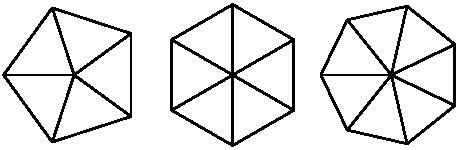
\includegraphics[scale=0.8]{figs/pies.pdf}}
\caption{Turtle pies.}
\label{fig.pies}
\end{figure}

\gr
ΑΣΚΗΣΗ 4.3
\index{pie}

Γράψτε ένα σύνολο κατάλληλων γενικών συναρτήσεων οι οποίες θα μπορούν να σχεδιάσουν
σχήματα όπως στην Εικόνα~\ref{fig.pies}.

Λύση\en : \url{http://thinkpython.com/code/pie.py}.

\gr
ΑΣΚΗΣΗ 4.4
\index{alphabet}
\index{turtle typewriter}
\index{typewriter, turtle}

Τα γράμματα του αγγλικού αλφαβήτου μπορούν να σχεδιαστούν από ένα μέτριο αριθμό βασικών στοιχείων,
όπως κάθετες και οριζόντιες γραμμές και μερικές καμπύλες. Σχεδιάστε μία γραμματοσειρά η οποία
μπορεί να υλοποιηθεί με ένα μικρό αριθμό βασικών στοιχείων και στη συνέχεια γράψτε συναρτήσεις
η οποίες θα σχεδιάζουν γράμματα του αγγλικού αλφαβήτου.

Πρέπει να γράψετε μία συνάρτηση για κάθε γράμμα, με ονόματα \en \verb"draw_a", \verb"draw_b", \gr κτλ.,
και βάλτε της συναρτήσεις σε ένα φάκελο με όνομα \en {\tt letters.py}. \gr Μπορείτε να κατεβάσετε μία
''χελώνα δακτυλογράφο'' από εδώ \en : \url{http://thinkpython.com/code/typewriter.py} \gr για να σας
βοηθήσει να ελέγξετε τον κώδικά σας.

Λύση\en : \url{http://thinkpython.com/code/letters.py}, \gr απαιτεί επίσης \en :
\url{http://thinkpython.com/code/polygon.py}.

\gr
ΑΣΚΗΣΗ 4.5

Διαβάστε σχετικά με τις σπείρες στο \en \url{http://en.wikipedia.org/wiki/Spiral}, \gr και στη συνέχεια
γράψτε ένα πρόγραμμα που θα σχεδιάζει μία Αρχιμήδεια σπείρα (ή ένα από τα υπόλοιπα είδη). Λύση\en : \url{http://thinkpython.com/code/spiral.py}.
\index{spiral}
\index{Archimedian spiral}
\gr


\chapter{Δηλώσεις υπό συνθήκη και αναδρομή}

\section{Τελεστής υπολογισμού υπολοίπου ακέραιας διαίρεσης}
\index{modulus operator}
\index{operator!modulus}

Ο τελεστής \en "\gr υπόλοιπο\en " \gr λειτουργεί σε ακέραιους αριθμούς και δίνει το υπόλοιπο όταν
ο πρώτος τελεστέος διαιρείται από το δεύτερο. Στην \en Python, \gr ο τελεστής \en "\gr υπόλοιπο\en " \gr  είναι το σύμβολο επί τοις
εκατό \en (\verb"%"). \gr Η σύνταξη είναι η ίδια όπως και με τους άλλους τελεστές\en :

\begin{verbatim}
>>> quotient = 7 / 3
>>> print quotient
2
>>> remainder = 7 % 3
>>> print remainder
1
\end{verbatim}
%
\gr
Έτσι το 7 διαιρούμενο με το 3 μας δίνει υπόλοιπο 1.

Ο τελεστής \en "\gr υπόλοιπο\en " \gr αποδεικνύεται εκπληκτικά χρήσιμος. Για παράδειγμα, μπορείτε να ελέγξετε αν ένας
αριθμός διαιρείται από έναν άλλο, εάν αυτό \en {\tt x \% y} \gr είναι μηδέν, τότε ο \en {\tt x} \gr διαιρείται από τον
\en {\tt y}.
\index{divisibility}

\gr
Επίσης, μπορείτε να εξάγετε το δεξιότερο ψηφίο ή ψηφία από έναν αριθμό. Για παράδειγμα, η \en {\tt x \% 10}
\gr δίνει το δεξιότερο ψηφίο της \en {\tt x} \gr (στη βάση του 10). Παρομοίως, η \en {\tt x \% 100} \gr δίνει τα δύο
τελευταία ψηφία.


\section{Λογικές εκφράσεις}
\index{boolean expression}
\index{expression!boolean}
\index{logical operator}
\index{operator!logical}

Μία λογική έκφραση είναι μία έκφραση η οποία είναι είτε αληθής ή ψευδής. Τα ακόλουθα παραδείγματα
χρησιμοποιούν τον τελεστή \en {\tt ==}, \gr ο οποίος συγκρίνει δύο τελεστέους και παράγει \en {\tt True} \gr
αν είναι ίσοι και \en {\tt False} \gr σε οποιαδήποτε άλλη περίπτωση\en :

\begin{verbatim}
>>> 5 == 5
True
>>> 5 == 6
False
\end{verbatim}
%
\gr
Η \en {\tt True} \gr και η \en {\tt False} \gr είναι ειδικές τιμές οι οποίες ανήκουν στον τύπο
\en {\tt bool}, \gr δεν είναι συμβολοσειρές\en :
\index{True special value}
\index{False special value}
\index{special value!True}
\index{special value!False}
\index{bool type}
\index{type!bool}

\begin{verbatim}
>>> type(True)
<type 'bool'>
>>> type(False)
<type 'bool'>
\end{verbatim}
%
\gr
Ο τελεστής \en {\tt ==} \gr  είναι ένας από τους σχεσιακούς τελεστές, οι άλλοι είναι:
\en
\begin{verbatim}
      x != y               # x is not equal to y
      x > y                # x is greater than y
      x < y                # x is less than y
      x >= y               # x is greater than or equal to y
      x <= y               # x is less than or equal to y
\end{verbatim}
%
\gr
Παρόλο που αυτές οι πράξεις σας είναι πιθανώς γνωστές, τα σύμβολα της \en Python
\gr είναι διαφορετικά από τα σύμβολα των μαθηματικών. Ένα σύνηθες λάθος είναι να χρησιμοποιείτε ένα μονό σύμβολο ισότητας
\en ({\tt =}) \gr αντί για διπλό σύμβολο ισότητας \en ({\tt ==}). \gr Να θυμάστε ότι το \en {\tt =} \gr είναι ένας τελεστής εκχώρησης και το \en {\tt ==} \gr είναι ένας σχεσιακός τελεστής. Δεν υπάρχει κάτι αντίστοιχο των \en {\tt =<} \gr και \en {\tt =>}.\gr
\index{relational operator}
\index{operator!relational}


\section{Λογικοί τελεστές}
\index{logical operator}
\index{operator!logical}

Υπάρχουν τρεις λογικοί τελεστές: ο \en {\tt and}, \gr ο \en {\tt or} \gr και ο \en {\tt not}. \gr
Η σημασιολογική ερμηνεία αυτών των τελεστών είναι παρόμοια με το νόημά τους στα Αγγλικά. Για παράδειγμα,
η \en " {\tt x > 0 and x < 10} " \gr είναι αληθής μόνο αν το \en {\tt x}  \gr είναι μεγαλύτερο του μηδενός και μικρότερο του 10.
\index{and operator}
\index{or operator}
\index{not operator}
\index{operator!and}
\index{operator!or}
\index{operator!not}

Η \en " {\tt n\%2 == 0 or n\%3 == 0} " \gr είναι αληθείς αν οποιαδήποτε από τις συνθήκες είναι αληθής, αυτό συμβαίνει αν ο αριθμός διαιρείται με το 2 ή με το 3.

Τέλος, ο  \en {\tt not} \gr τελεστής ακυρώνει μια λογική έκφραση, έτσι η \en " {\tt not (x > y)} " \gr είναι
αληθής αν ο \en {\tt x > y} \gr είναι λάθος, αυτό συμβαίνει αν το \en {\tt x}  \gr είναι μικρότερος ή ίσος του \en {\tt y}.

\gr
Στην κυριολεξία, οι τελεστέοι των λογικών τελεστών θα πρέπει να είναι λογικές εκφράσεις, αλλά η \en Python \gr
δεν είναι τόσο αυστηρή. Κάθε μη μηδενικός αριθμός διερμηνεύεται ως \en "\gr αληθής\en " (''true'').

\begin{verbatim}
>>> 17 and True
True
\end{verbatim}
%
\gr
Αυτή η ευελιξία μπορεί να είναι χρήσιμη, αλλά υπάρχουν κάποιες λεπτομέριες που μπορεί να προκαλέσουν σύγχυση.
Καλύτερα να το αποφύγετε (εκτός αν ξέρετε τι κάνετε).


\section{Εκτέλεση υπό συνθήκη}
\label{conditional.execution}

\index{conditional statement}
\index{statement!conditional}
\index{if statement}
\index{statement!if}
\index{conditional execution}

Προκειμένου να γράψουμε χρήσιμα προγράμματα, σχεδόν πάντα χρειαζόμαστε τη δυνατότητα
να ελέγχουμε συνθήκες και να αλλάζουμε αναλόγως τη συμπεριφορά του προγράμματος.
Οι \en "\gr δηλώσεις υπό συνθήκη\en " \gr μας δίνουν αυτή τη δυνατότητα. Η απλούστερη μορφή είναι η δήλωση
\en {\tt if}:

\begin{verbatim}
if x > 0:
    print 'x is positive'
\end{verbatim}
%
\gr
Η λογική έκφραση μετά την \en  {\tt if} \gr ονομάζεται συνθήκη. Αν είναι αληθής, τότε η
εμφωλευμένη δήλωση αρχίζει να εκτελείται. Αν όχι, δε γίνεται τίποτα.
\index{condition}
\index{compound statement}
\index{statement!compound}

Οι δηλώσεις \en {\tt if} \gr έχουν την ίδια δομή με τους ορισμούς συνάρτησης:
μία επικεφαλίδα ακολουθούμενη από ένα εμφωλευμένο σώμα. Δηλώσεις όπως αυτές
ονομάζονται σύνθετες δηλώσεις.

Δεν υπάρχει όριο στον αριθμό των δηλώσεων που μπορούν να εμφανιστούν στο σώμα,
αλλά πρέπει να υπάρχει τουλάχιστον μία.
Ενίοτε, είναι χρήσιμο να έχετε ένα σώμα χωρίς δηλώσεις (συνήθως σαν ένα κρατημένο μέρος
για τον κώδικα που δεν έχετε γράψει ακόμη). Σε αυτή τη περίπτωση, μπορείτε να χρησιμοποιήσετε τη
δήλωση \en {\tt pass}, \gr η οποία δεν κάνει τίποτα.
\index{pass statement}
\index{statement!pass}
\en
\begin{verbatim}
if x < 0:
    pass          # need to handle negative values!
\end{verbatim}
%
\gr
\section{Εναλλακτική εκτέλεση}
\label{alternative.execution}
\index{alternative execution}
\index{else keyword}
\index{keyword!else}

Μία δεύτερη μορφή της δήλωσης \en {\tt if} \gr είναι η εναλλακτική εκτέλεση, στην οποία
υπάρχουν δύο ενδεχόμενα και η συνθήκη καθορίζει ποιο θα εκτελεστεί. Η σύνταξη μοιάζει κάπως έτσι\en :

\begin{verbatim}
if x%2 == 0:
    print 'x is even'
else:
    print 'x is odd'
\end{verbatim}
%
\gr
Αν το υπόλοιπο της διαίρεσης του \en {\tt x} \gr με το 2 είναι 0, τότε καταλαβαίνουμε πως το \en
{\tt x} \gr είναι άρτιος, και το πρόγραμμα εμφανίζει ένα μήνυμα γι αυτό το αποτέλεσμα. Αν η συνθήκη είναι ψευδής, εκτελείται
το δεύτερο σύνολο δηλώσεων. Από τη στιγμή που η συνθήκη μπορεί να είναι αληθής ή ψευδής, ακριβώς μόνο μία από τις
εναλλακτικές θα εκτελεστεί. Οι εναλλακτικές ονομάζονται κλάδοι, επειδή είναι κλάδοι \en ({\bf branches}) \gr στη ροή εκτέλεσης.
\index{branch}


\gr
\section{Αλυσιδωτές συνθήκες}
\index{chained conditional}
\index{conditional!chained}

Κάποιες φορές χρειαζόμαστε περισσότερους από δύο κλάδους γιατί υπάρχουν περισσότερες από δύο πιθανότητες.
Ένας τρόπος για να εκφράσουμε έναν τέτοιο υπολογισμό είναι μία αλυσιδωτή συνθήκη\en :

\begin{verbatim}
if x < y:
    print 'x is less than y'
elif x > y:
    print 'x is greater than y'
else:
    print 'x and y are equal'
\end{verbatim}
%
\gr
Η \en {\tt elif} \gr  είναι μία συντομογραφία της \en ``else if''. \gr Και πάλι, ακριβώς ένας
κλάδος θα εκτελεστεί. Δεν υπάρχει όριο στον αριθμό των \en {\tt elif} \gr δηλώσεων. Αν υπάρχει μία
πρόταση \en {\tt else}, \gr θα πρέπει να βρίσκεται στο τέλος, αλλά δεν είναι απαραίτητο να υπάρχει.
\index{elif keyword}
\index{keyword!elif}

\en
\begin{verbatim}
if choice == 'a':
    draw_a()
elif choice == 'b':
    draw_b()
elif choice == 'c':
    draw_c()
\end{verbatim}
%
\gr
Η κάθε συνθήκη ελέγχεται με τη σειρά. Αν η πρώτη είναι λάθος, ελέγχεται η δεύτερη και
ούτω καθεξής. Αν μία από αυτές είναι αληθής, εκτελείται ο αντίστοιχος κλάδος και η δήλωση
τερματίζει. Ακόμη κι αν περισσότερες από μία συνθήκη είναι αληθείς, μόνο ο πρώτος αληθής
κλάδος εκτελείται.


\section{Εμφωλευμένες συνθήκες}
\index{nested conditional}
\index{conditional!nested}

Ένας όρος μπορεί επίσης να είναι εμφωλευμένος μέσα σε έναν άλλο. Επομένως, θα μπορούσαμε να είχαμε
γράψει το παράδειγμα της τριχοτόμησης κάπως έτσι\en :

\begin{verbatim}
if x == y:
    print 'x and y are equal'
else:
    if x < y:
        print 'x is less than y'
    else:
        print 'x is greater than y'
\end{verbatim}
%
\gr
Η εξωτερική συνθήκη περιέχει δύο κλάδους. Ο πρώτος κλάδος περιέχει μία απλή δήλωση.
Ο δεύτερος κλάδος περιέχει μία άλλη δήλωση \en {\tt if} \gr η οποία έχει δύο κλάδους από μόνη της.
Αυτοί οι δύο κλάδοι είναι απλές δηλώσεις, παρόλο που θα μπορούσαν επίσης να είναι δηλώσεις υπό συνθήκη.

Παρόλο που η ενδοπαραγραφοποίηση των δηλώσεων κάνει τη δομή εμφανή, οι εμφωλευμένες
συνθήκες δεν ειναι εύκολο να διαβαστούν γρήγορα. Γενικά, είναι καλή ιδέα να τις αποφεύγετε
όποτε μπορείτε.

Οι λογικοί τελεστές παρέχουν συχνά ένα τρόπο για την απλοποίηση των εμφωλευμένων
δηλώσεων υπό συνθήκη. Για παράδειγμα, μπορούμε να γράψουμε ξανά τον ακόλουθο κώδικα
χρησιμοποιώντας μία απλή υπόθεση\en :

\begin{verbatim}
if 0 < x:
    if x < 10:
        print 'x is a positive single-digit number.'
\end{verbatim}
%
\gr
Η δήλωση \en {\tt print} \gr εκτελείται μόνο αν είναι αληθείς και οι δυο συνθήκες,
έτσι μπορούμε να έχουμε το ίδιο απότελεσμα με τον τελεστή \en {\tt and}\en :

\begin{verbatim}
if 0 < x and x < 10:
    print 'x is a positive single-digit number.'
\end{verbatim}

\gr
\section{Αναδρομή}
\label{recursion}
\index{recursion}

\gr
Είναι έγκυρο μία συνάρτηση να καλεί μία άλλη αλλά είναι επίσης έγκυρο μία συνάρτηση να καλεί τον εαυτό της.
Ίσως να μην είναι προφανές για ποιο λόγο αυτό ειναι χρήσιμο, αλλά αποδεικνύεται ένα από τα πιο μαγικά πράγματα που
μπορεί να κάνει ένα πρόγραμμα. Για παράδειγμα, δείτε την ακόλουθη συνάρτηση\en :

\begin{verbatim}
def countdown(n):
    if n <= 0:
        print 'Blastoff!'
    else:
        print n
        countdown(n-1)
\end{verbatim}
%
\gr
Αν η \en {\tt n} \gr είναι 0 ή αρνητική, στην έξοδο πέρνουμε τη λέξη \en ``Blastoff!'' \gr
Αλλιώς, η έξοδος είναι η τιμή της \en {\tt n} \gr και στη συνέχεια καλείται μία συνάρτηση με όνομα \en
{\tt countdown}\gr , η οποία από μόνη της περνάει τη έκφραση \en {\tt n-1} \gr σαν όρισμα.

Τί συμβαίνει αν καλέσουμε αυτή τη συνάρτηση με αυτό τον τρόπο\en :

\begin{verbatim}
>>> countdown(3)
\end{verbatim}
%
\gr
Η εκτέλεση της \en {\tt countdown} \gr ξεκινάει με \en {\tt n=3}, \gr και από τη στιγμή
που η \en {\tt n} \gr είναι μεγαλύτερη του 0, έχει σαν έξοδο την τιμή 3 και έπειτα καλεί τον εαυτό της...

\begin{quote}
Η εκτέλεση της \en {\tt countdown} \gr ξεκινάει με \en {\tt n=2}, \gr και από τη στιγμή που η
\en {\tt n} \gr είναι μεγαλύτερη του 0, έχει σαν έξοδο την τιμή 2 και έπειτα καλεί τον εαυτό της...

\begin{quote}
Η εκτέλεση της \en {\tt countdown} \gr ξεκινάει με \en {\tt n=1}, \gr και από τη στιγμή που η
\en {\tt n} \gr είναι μεγαλύτερη του 0, έχει σαν έξοδο την τιμή 1 και έπειτα καλεί τον εαυτό της...

\begin{quote}
Η εκτέλεση της \en {\tt countdown} \gr ξεκινάει με τη \en {\tt n=0}, \gr και από τη στιγμή που η
\en {\tt n} \gr δεν είναι μεγαλύτερη του 0, έχει σαν έξοδο τη λέξη \en ``Blastoff!' \gr και έπειτα επιστρέφει.
\end{quote}

Η \en {\tt countdown} \gr που πήρε \en {\tt n=1} \gr επιστρέφει.
\end{quote}

Η  \en {\tt countdown} \gr που πήρε \en {\tt n=2} \gr επιστρέφει.
\end{quote}

Η  \en {\tt countdown} \gr που πήρε \en {\tt n=3} \gr επιστρέφει.

Και έπειτα βρίσκεστε πίσω στη \en \verb"__main__". \gr Έτσι, η συνολική έξοδος
είναι κάπως έτσι\en :

\begin{verbatim}
3
2
1
Blastoff!
\end{verbatim}
%
\gr
Μία συνάρτηση η οποία καλεί τον εαυτό της ονομάζεται αναδρομική συνάρτηση και η διαδικασία
ονομάζεται αναδρομή.
\index{recursion}
\index{function!recursive}

Σαν άλλο παράδειγμα, μπορούμε να γράψουμε μία συνάρτηση η οποία εμφανίζει μία συμβολοσειρά \en
{\tt n} \gr φορές.

\en
\begin{verbatim}
def print_n(s, n):
    if n <= 0:
        return
    print s
    print_n(s, n-1)
\end{verbatim}
%
\gr
Αν \en {\tt n <= 0} \gr η δήλωση \en {\tt return} \gr τερματίζει τη συνάρτηση. Η ροή εκτέλεσης επιστρέφει
αμέσως στην συνάρτηση που την κάλεσε, και οι υπόλοιπες γραμμές της συνάρτησης δεν εκτελούνται.
\index{return statement}
\index{statement!return}

Η υπόλοιπη συνάρτηση είναι παρόμοια με τη \en {\tt countdown}: \gr
εάν η \en {\tt n} \gr είναι μεγαλύτερη του 0, εμφανίζει τη \en {\tt s} \gr και μετά καλεί τον
εαυτό της για να εμφανίσει την \en "{\tt s}" $n-1$ \gr επιπλέον φορές. Έτσι ο αριθμός γραμμών της εξόδου
είναι \en {\tt 1 + (n - 1)}, \gr ο οποίος είναι ίσος με \en {\tt n}.\gr

Για απλά παραδείγματα όπως αυτά, είναι πιθανώς ευκολότερο να χρησιμοποιήσετε ένα βρόγχο \en {\tt for}.    \gr
Αλλά θα δούμε αργότερα παραδείγματα τα οποία είναι δύσκολο να γραφούν με ένα βρόγχο \en {\tt for} \gr και εύκολο να γραφούν με αναδρομή,
γι αυτό το λόγο είναι καλό να ξεκινήσετε νωρίς.



\section{Διαγράμματα στοίβας για αναδρομικές συναρτήσεις}
\label{recursive.stack}
\index{stack diagram}
\index{function frame}
\index{frame}

Στην παράγραφο\en ~\ref{stackdiagram}, \gr χρησιμοποιήσαμε ένα διάγραμμα στοίβας για να
αναπαραστήσουμε τη κατάσταση του προγράμματος κατά τη διάρκεια μιας κλήσης συνάρτησης. Το ίδιο είδος
διαγράμματος μπορεί να βοηθήσει για να ερμηνεύσουμε μια αναδρομική συνάρτηση.

Κάθε φορά που καλείται μία συνάρτηση. Η \en Python \gr δημιουργεί ένα καινούργιο πλαίσιο συνάρτησης,
το οποίο περιέχει τις τοπικές μεταβλητές και τις παραμέτρους της συνάρτησης. Για μία αναδρομική συνάρτηση,
μπορεί να υπάρχουν την ίδια στιγμή, περισσότερα από ένα πλαισιο στη στοίβα.

Εικόνα\en ~\ref{fig.stack2} \gr δείχνει ένα διάγραμμα στοίβας για τη \en {\tt countdown} \gr η οποία έχει καλεστεί με \en {\tt n = 3}.\gr

\begin{figure}
\centerline
{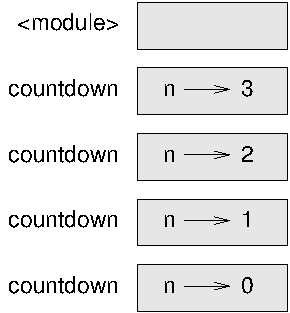
\includegraphics[scale=0.8]{figs/stack2.pdf}}
\caption{Διάγραμμα στοίβας.}
\label{fig.stack2}
\end{figure}

\gr
Ως συνήθως, στη κορυφή της στοίβας είναι το πλαίσιο για τη \en \verb"__main__". \gr Είναι άδειο γιατί
δε δημιουργήσαμε μεταβλητές στη \en \verb"__main__" \gr ούτε της περάσαμε κάποιο όρισμα.
\index{base case}
\index{recursion!base case}

Τα τέσσερα πλαίσια \en {\tt countdown} \gr έχουν διαφορετικές τιμές για την παράμετρο \en {\tt n}. \gr
Στο κάτω μέρος της στοίβας, όπου \en {\tt n=0}, \gr ονομάζεται περίπτωση βάσης. Δεν κάνει αναδρομική κλήση, γι αυτό
δεν υπάρχουν άλλα πλαίσια.

ΑΣΚΗΣΗ 5.1

Σχεδιάστε ένα διάγραμμα στοίβας για τη \en \verb"print_n" \gr η οποία θα καλείται με \en \verb"s = 'Hello'" \gr και \en {\tt n=2}.
\gr

ΑΣΚΗΣΗ 5.2

Γράψτε μία συνάρτηση με όνομα \en \verb"do_n"  \gr η οποία παίρνει ένα αντικείμενο συνάρτησης και έναν αριθμό \en {\tt n} \gr ως
ορίσματα και καλεί τη δοθείσα συνάρτηση \en {\tt n} \gr φορές.



\section{Άπειρη αναδρομή}
\index{infinite recursion}
\index{recursion!infinite}
\index{runtime error}
\index{error!runtime}
\index{traceback}

Αν μία αναδρομή δε φτάνει ποτε σε μία περίπτωση βάσης, συνεχίζει κάνοντας αναδρομικές κλήσεις για πάντα και αυτό το
πρόγραμμα δεν τερματίζει ποτέ. Είναι γνωστή ως άπειρη αναδρομή, και δεν είναι καλή ιδέα γενικώς. Αυτό είναι ένα
πολύ μικρό πρόγραμμα με άπειρη αναδρομή\en :

\begin{verbatim}
def recurse():
    recurse()
\end{verbatim}
%
\gr
Στα περισσότερα προγραμματιστικά περιβάλλοντα, ένα πρόγραμμα με άπειρη αναδρομή δεν τρέχει για πάντα. Η \en Python \gr
αναφέρει ένα μήνυμα λάθους αν φτάσει στο μέγιστο βάθος αναδρομής\en :
\index{exception!RuntimeError}
\index{RuntimeError}

\begin{verbatim}
  File "<stdin>", line 2, in recurse
  File "<stdin>", line 2, in recurse
  File "<stdin>", line 2, in recurse
                  .
                  .
                  .
  File "<stdin>", line 2, in recurse
RuntimeError: Maximum recursion depth exceeded
\end{verbatim}
%
\gr
Αυτή η αναδρομή είναι λίγο μεγαλύτερη από αυτή που είδαμε στο προηγούμενο κεφάλαιο.
Όταν συμβεί το λάθος, υπάρχουν 1000 αναδρομικά πλαίσια στη στοίβα\en !\gr


\section{Είσοδος από το πληκτρολόγιο}
\index{keyboard input}

Τα προγράμματα που έχουμε γράψει μέχρι στιγμής είναι λίγο αγενή με την έννοια ότι δε δέχονται
καμία είσοδο από το χρήστη. Απλώς κάνουν το ίδιο πράγμα κάθε φορά.

Η \en Python 2 \gr παρέχει μία ενσωματωμένη συνάρτηση με όνομα \en \verb"raw_input" \gr η οποία παίρνει
είσοδο από το πληκτρολόγιο. Στην \en Python 3, \gr έχει όνομα \en {\tt input}. \gr 'Οταν καλείται αυτή η συνάρτηση,
το πρόγραμμα σταματάει και περιμένει το χρήστη να πληκτρολογήσει κάτι. Όταν ο χρήστης πατάει \en {\sf Return} \gr ή
\en {\sf Enter}, \gr το πρόγραμμα συνεχίζει και η \en \verb"raw_input" \gr επιστρέφει ότι πληκτρολόγησε ο χρήστης σαν μία
συμβολοσειρά.\en
\index{Python 3}
\index{raw\_input function}
\index{function!raw\_input}

\begin{verbatim}
>>> text = raw_input()
What are you waiting for?
>>> print text
What are you waiting for?
\end{verbatim}
%
\gr
Πριν το πρόγραμμα πάρει την είσοδο από το χρήστη, είναι καλό να εμφανίζει ένα μήνυμα προτροπής
το οποίο θα λέει στο χρήστη τι να εισάγει. Η \en \verb"raw_input" \gr μπορεί να πάρει σαν όρισμα
ένα τέτοιο μήνυμα\en :
\index{prompt}

\begin{verbatim}
>>> name = raw_input('What...is your name?\n')
What...is your name?
Arthur, King of the Britons!
>>> print name
Arthur, King of the Britons!
\end{verbatim}
%
\gr
Το \en \verb"\n" \gr στο τέλος του μηνύματος αναπαριστά μία \en {\bf newline}\gr ,
ο οποίος είναι ένας ειδικός χαρακτήρας που προκαλεί αλλαγή γραμμής.
Για αυτό η είσοδος του χρήστη εμφανίζεται κάτω από το μήνυμα προτροπής.
\index{newline}

Εάν περιμένετε ο χρήστης να πληκτρολογήσει έναν ακέραιο, μπορείτε να δοκιμάσετε να
μετατρέψετε την επιστρεφόμενη τιμή σε \en {\tt int}:

\begin{verbatim}
>>> prompt = 'What...is the airspeed velocity of an unladen swallow?\n'
>>> speed = raw_input(prompt)
What...is the airspeed velocity of an unladen swallow?
17
>>> int(speed)
17
\end{verbatim}
%
\gr
Αλλά αν ο χρήστης πληκτρολογήσει κάτι διαφορετικό από μία σειρά ψηφίων, θα
πάρετε ένα μήνυμα λάθους\en :

\begin{verbatim}
>>> speed = raw_input(prompt)
What...is the airspeed velocity of an unladen swallow?
What do you mean, an African or a European swallow?
>>> int(speed)
ValueError: invalid literal for int()
\end{verbatim}
%
\gr
Θα δούμε πώς χειριζόμαστε τέτοιου είδους λάθη αργότερα.
\index{ValueError}
\index{exception!ValueError}


\section{Αποσφαλμάτωση}
\label{whitespace}
\index{debugging}
\index{traceback}

Η \en Python \gr εμφανίζει αναδρομικά πολλές πληροφορίες όταν συμβεί κάποιο λάθος,
κάτι το οποίο μπορεί να είναι υπερβολικό, ειδικά όταν υπάρχουν πολλά πλαίσια στη στοίβα.
Τα πιο χρήσιμα σημεία είναι συνήθως\en :

\begin{itemize}

\item What kind of error it was, and

\item Where it occurred.

\end{itemize}
\gr
Τα συντακτικά λάθη είναι συνήθως εύκολο να τα βρέθούν, αλλά υπάρχουν μερικές
παγίδες. Τα λάθη λευκού κενού διαστήματος \en (whitespace errors) \gr μπορεί να είναι
δυσεπίλυτα γιατί τα κενά διαστήματα\en (spaces) \gr και οι στηλοθέτες\en (tabs) \gr
είναι αόρατα και συνηθίζουμε να τα αγνοούμε. \en
\index{whitespace}

\begin{verbatim}
>>> x = 5
>>>  y = 6
  File "<stdin>", line 1
    y = 6
    ^
SyntaxError: invalid syntax
\end{verbatim}
%
\gr
Σε αυτό το παράδειγμα, το πρόβλημα είναι ότι η δεύτερη γραμμή έχει
εσοχή ενός κενού διαστήματος. Αλλά το μήνυμα λάθους δείχνει το \en {\tt y}\gr ,
το οποίο είναι παραπλανητικό. Σε γενικές γραμμές, τα μηνύματα λάθους υποδεικνύουν
που ανακαλύφθηκε το πρόβλημα, αλλά το πραγματκό λάθος μπορεί να είναι νωρίτερα στον
κώδικα, ακόμη και σε μία προηγούμενη γραμμή.
\index{error!runtime}
\index{runtime error}

Το ίδιο ισχύει και για τα λάθη χρόνου εκτέλεσης.

Υποθέστε ότι προσπαθείτε να υπολογίσετε ένα σηματοθορυβικό λόγο σε ντεσιμπέλ \en (dB) \gr .
Ο τύπος είναι $SNR_{db} = 10 \log_{10} (P_{signal} / P_{noise})$. Στην \en Python\gr , ίσως το
γράφατε κάπως έτσι\en :

\begin{verbatim}
import math
signal_power = 9
noise_power = 10
ratio = signal_power / noise_power
decibels = 10 * math.log10(ratio)
print decibels
\end{verbatim}
%
\gr
Αλλά όταν το τρέχετε στην \en Python 2,\gr παίρνετε ένα μήνυμα λάθους. \en
\index{exception!OverflowError}
\index{OverflowError}

\begin{verbatim}
Traceback (most recent call last):
  File "snr.py", line 5, in ?
    decibels = 10 * math.log10(ratio)
OverflowError: math range error
\end{verbatim}
%
\gr
Το μήνυμα λάθους υποδεικνύει την γραμμή 5, αλλά δεν υπάρχει
κάτι λάθος σε αυτήν τη γραμμή. Για να βρούμε το πραγματικό λάθος,
ίσως θα ήταν χρήσιμο να εμφανίζαμε την τιμή της \en {\tt ratio}\gr ,
η οποία αποδεικνύεται ότι είναι 0. Το πρόβλημα είναι στη γραμμή 4,
επειδή όταν διαιρούμε δύο ακέραιους αριθμούς έχουμε ακέραια διαίρεση.
Η λύση είναι να αναπαραστήσουμε την ισχύ του σήματος και την ισχύ του
θορύβου με αριθμούς κινητής υποδιαστολής.
\index{floor division}
\index{division!floor}

Γενικά, τα μηνύματα λάθους σας λένε που ανακαλύφθηκε το πρόβλημα, αλλά
συχνά αυτό δεν είναι και το που προκλήθηκε.

Στην \en Python 3\gr , αυτό το παράδειγμα δεν προκαλεί σφάλμα, γιατί ο τελεστής
της διαίρεσης εκτελεί δεκαδική διαίρεση ακόμα και με ακέραιους τελεστέους.


\section{Ορολογία}

\begin{description}

\item[τελεστής υπολογισμού υπολοίπου ακέραιας διαίρεσης:] Ένας τελεστής,
ο οποίος συμβολίζεται με το επί της εκατό συμβολο \en ({\tt \%})\gr . Δουλεύει
με ακεραίους και επιστρέφει το υπόλοιπο όταν διαιρέσουμε έναν αριθμό με κάποιον
άλλον.
\index{modulus operator}
\index{operator!modulus}

\item[λογική έκφραση:]  Μία έκφραση της οποίας η τιμή είναι είτε αληθής \en ({\tt True}) \gr
είτε ψευδής \en ({\tt False}).\gr
\index{boolean expression}
\index{expression!boolean}

\item[σχεσιακός τελεστής:]  Ένας τελεστής ο οποίος συγκρίνει δύο τελεστέους: \en
{\tt ==}, {\tt !=}, {\tt >}, {\tt <}, {\tt >=}, \gr και \en {\tt <=}.\gr

\item[λογικός τελεστής:]  Ένας τελεστής ο οποίος συνενώνει δύο λογικές εκφράσεις: \en
{\tt and}, {\tt or} \gr και \en {\tt not}.\gr

\item[δηλώσεις υπό συνθήκη:]  Μία δήλωση η οποία ελέγχει τη ροή εκτέλεσης ανάλογα με
κάποια συνθήκη.
\index{conditional statement}
\index{statement!conditional}

\item[συνθήκη:]  Η λογική έκφραση σε μία υπό συνθήκη δήλωση η οποία καθορίζει ποιος
κλάδος θα εκτελεστεί.
\index{condition}

\item[σύνθετη δήλωση:]  Μία δήλωση η οποία αποτελείται από μία επικεφαλίδα και
ένα σώμα. Η επικεφαλίδα τελιώνει με μία άνω και κάτω τελεία \en (:)\gr . Και το σώμα
είναι γραμμένο σε εσοχή σχετικά με την επικεφαλίδα.
\index{compound statement}

\item[κλάδος:] Μία από τις εναλλακτικές ακολουθίες εντολών σε μία υπό συνθήκη
δήλωση.
\index{branch}

\item[αλυσιδωτές συνθήκες:]  Μία υπό συνθήκη δήλωση με μια σειρά εναλλακτικών
κλάδων.
\index{chained conditional}
\index{conditional!chained}

\item[εμφωλευμένη συνθήκη:]  Μία υπό συνθήκη δήλωση η οποία εμφανίζεται σε
έναν από τους κλάδους μίας άλλης υπό συνθήκης δήλωσης.
\index{nested conditional}
\index{conditional!nested}

\item[αναδρομή:]  Η διαδικασία κατά την οποία καλείται η συνάρτηση η οποία
τρέχει αυτή τη στιγμή.
\index{recursion}

\item[περίπτωση βάσης:]  Ένας υπό συνθήκη κλάδος σε μία αναδρομική συνάρτηση
ο οποίος δεν κάνει καμία αναδρομική κλήση.
\index{base case}

\item[άπειρη αναδρομή:]  Μία αναδρομή η οποία δεν έχει περίπτωση βάσης ή δεν
την φτάνει ποτέ (δηλαδή δεν την επαληθεύει). Και τελικά, μία άπειρη αναδρομή προκαλεί
ένα λάθος χρόνου εκτέλεσης.
\index{infinite recursion}

\end{description}

\section{Ασκήσεις}

ΑΣΚΗΣΗ 5.1
\index{Fermat's Last Theorem}

Το τελευταίο θεώρημα του \en Fermat \gr λέει ότι δεν υπάρχουν ακέραιοι $a$, $b$, και
$c$ τέτοιοι ώστε

\[ a^n + b^n = c^n \]
%
για οποιαδήποτε τιμή του $n$ μεγαλύτερη του 2.

\begin{enumerate}

\item Γράψτε μία συνάρτηση με όνομα \en \verb"check_fermat" \gr η οποία
θα παίρνει 4 παραμέτρους, \en {\tt a}, {\tt b}, {\tt c} \gr και \en {\tt n}, \gr και
και θα ελέγχει αν ισχύει το θεώρημα του \en Fermat. \gr Αν το $n$ είναι μεγαλύτερο
του 2 και αποδεικνύεται ότι η σχέση

\[a^n + b^n = c^n \]
%
είναι αληθής, το πρόγραμμα θα πρέπει να εμφανίζει το μύνημα\en :
``Holy smokes, Fermat was wrong!'' \gr Αλλιώς θα εμφανίζει\en :
``No, that doesn't work.''\gr

\item Γράψτε μία συνάρτηση η οποία ζητάει από το χρήστη να εισάγει τιμές
για τις \en {\tt a}, {\tt b}, {\tt c} \gr και \en {\tt n}, \gr τις μετατρέπει
σε ακέραιους και χρησιμοποιεί την \en \verb"check_fermat" \gr για να ελέγξεί αν
παραβιάζουν το θεώρημα του \en Fermat.\gr

\end{enumerate}



ΑΣΚΗΣΗ 5.2
\index{triangle}

Αν σας δωθούν τρία ξυλάκια, ίσως μπορείτε να σχηματίσετε ένα τρίγωνο με αυτά,
ίσως και όχι. Για παράδειγμα, εάν ένα από τα ξυλάκια είναι 12 εκατοστά και τα
άλλα δύο είναι 1 εκατοστο το καθένα, είναι προφανές ότι δεν θα είστε σε θέση
να ενώσετε τα κοντά ξυλάκια μεταξύ τους. Μπορούμε να κάνουμε μία απλή δοκιμή
για οποιαδήποτε τριάδα μηκών, ούτως ώστε να δουμε αν είναι εφικτό να σχηματίσουν
ένα τρίγωνο\en :

\begin{quotation}
\gr
Εάν ένα από τα τρία μήκη είναι μεγαλύτερο από το άθροισμα των άλλων δύο,
  τότε δεν μπορείτε να σχηματίσετε ένα τρίγωνο, αλλιώς μπορείτε.  \en (\gr
    Αν το άθροισμα δύο μηκών είναι ίσο με το τρίτο, σχηματίζουν ένα \en "\gr
    εκφυλισμένο\en "\gr τρίγωνο.\en )
\end{quotation}

\begin{enumerate}
\gr

\item Γράψτε μία συνάρτηση με όνομα \en \verb"is_triangle" \gr η οποία θα
  παίρνει τρεις ακέραιους σαν ορίσματα και θα εμφανίζει στην έξοδο είτε \en
  ``Yes'' \gr είτε \en ``No,'' \gr ανάλογα με το αν μπορείτε ή όχι να σχηματίσετε
  ένα τρίγωνο με τα ξυλάκια των δοθέντων μηκών.

\item Γράψτε μία συνάρτηση η οποία ζητάει από το χρήστη να εισάγει τρία
  μήκη για ξυλάκια, τα μετατρέπει σε ακέραιους και χρησιμοποιεί την \en
  \verb"is_triangle" \gr για να ελέγξει εάν τα ξυλάκια με τα δοθέντα μήκη
  μπορούν να σχεδιάσουν ένα τρίγωνο.

\end{enumerate}
\gr

Οι ακόλουθες ασκήσεις χρηιμοποιούν την \en TurtleWorld \gr από το Κεφάλαιο\en ~\ref{turtlechap}:
\index{TurtleWorld}
\gr

ΑΣΚΗΣΗ 5.3

Διαβάστε την παρακάτω συνάρτηση και δείτε αν μπορείτε να καταλάβετε τι κάνει.
Στη συνέχεια τρέξτε την \en (\gr δείτε τα παραδείγματα στο Κεφάλαιο\en ~\ref{turtlechap}).

\begin{verbatim}
def draw(t, length, n):
    if n == 0:
        return
    angle = 50
    fd(t, length*n)
    lt(t, angle)
    draw(t, length, n-1)
    rt(t, 2*angle)
    draw(t, length, n-1)
    lt(t, angle)
    bk(t, length*n)
\end{verbatim}



\begin{figure}
\centerline
{
\includegraphics[scale=0.8]{figs/koch.pdf}}
\caption{A Koch curve.}
\label{fig.koch}
\end{figure}

\gr ΑΣΚΗΣΗ 5.4
\index{Koch curve}

Η καμπύλη του \en Koch \gr είναι ένα φράκταλ το οποίο είναι όπως αυτό
στην Εικόνα\en ~\ref{fig.koch}. \gr Για να σχεδιάσετε μία καμπύλη του \en
Koch \gr με μήκος $χ$, το μόνο που έχετε να κάνετε είναι\en :

\begin{enumerate}
\gr

\item Σχεδιάστε μία καμπύλη του \en Koch \gr με μήκος $x/3$.

\item Στρίψτε αριστερά 60 μοίρες.

\item Σχεδιάστε μία καμπύλη του \en Koch \gr με μήκος $x/3$.

\item Στρίψτε δεξιά 120 μοίρες.

\item Σχεδιάστε μία καμπύλη του \en Koch \gr με μήκος $x/3$.

\item Στρίψτε αριστερά 60 μοίρες.

\item Σχεδιάστε μία καμπύλη του \en Koch \gr με μήκος $x/3$.

\end{enumerate}
\gr
Η εξαίρεση είναι εάν το $x$ είναι μικρότερο του 3\en : \gr
σε αυτήν την περίπτωση μπορείτε απλά να σχεδιάσετε μία ευθεία
γραμμή με μήκος $x$.

\begin{enumerate}

\item Γράψτε μία συνάρτηση με όνομα \en {\tt koch} \gr η οποία θα παίρνει
μία χελώνα και ένα μήκος σαν παραμέτρους, και χρησιμοποιεί τη χελώνα για να
σχεδιάσει μία καμπύλη του \en Koch \gr με το δοθέν μήκος.

\item Γράψτε μία συνάρτηση με όνομα \en {\tt snowflake} \gr η οποία θα σχεδιάζει
τρεις καμπύλες του \en Koch \gr για να φτιάξει το περίγραμμα μίας νιφάδας χιονιού.

Λύση\en : \url{http://thinkpython.com/code/koch.py}.\gr

\item Η καμπύλη του \en Koch \gr μπορεί να γενικευθεί με διάφορους τρόπους.
Δείτε εδώ\en : \url{http://en.wikipedia.org/wiki/Koch_snowflake} \gr κάποια
παραδείγματα και υλοποιήστε όποιο σας αρέσει.

\end{enumerate}


\chapter{Γόνιμες Συναρτήσεις}
\label{fruitchap}

\section{Επιστρεφόμενες τιμές}
\index{return value}

Μερικές από τις ενσωματωμένες συναρτήσεις που έχουμε χρησιμοποιήσει, όπως οι
μαθηματικές συναρτήσεις, παράγουν αποτελέσματα. Καλώντας τη συνάρτηση δημιουργείται
μία τιμή, την οποία συνήθως την εκχωρούμε σε μία μεταβλητή ή τη χρησιμοποιούμε ως μέρος
μίας εκφρασης.
\en
\begin{verbatim}
e = math.exp(1.0)
height = radius * math.sin(radians)
\end{verbatim}
%
\gr
Όλες οι συναρτήσεις που έχουμε γράψει μέχρι τώρα είναι κενές \en (void). \gr
Εμφανίζουν κάτι στην έξοδο ή μετακινούν χελώνες, αλλά η επιστρεφόμενη τιμή τους
είναι \en {\tt None}. \gr

Σε αυτό το κεφάλαιο, θα γράψουμε (επιτέλους) γόνιμες \en (fruitful) \gr συναρτήσεις.
Το πρώτο παράδειγμα είναι η \en {\tt area}\gr , η οποία επιστρέφει το εμβαδόν ενός κύκλου
με τη δοθείσα ακτίνα\en :

\begin{verbatim}
def area(radius):
    temp = math.pi * radius**2
    return temp
\end{verbatim}
%
\gr
Έχουμε ξαναδεί τη δήλωση \en {\tt return} \gr και νωρίτερα, αλλά σε μία γόνιμη
συνάρτηση η δήλωση \en {\tt return} \gr περιλαμβάνει μία έκφραση. Αυτή η δήλωση σημαίνει\en :
"\gr Επέστρεψε αμέσως από αυτή τη συνάρτηση και χρησιμοποίησε την ακόλουθη έκφραση σαν
επιστρεφόμενη τιμη\en ." \gr Η έκφραση μπορεί να είναι αυθαίρετα πολύπλοκη, έτσι θα μπορούσαμε
να είχαμε γράψει αυτή τη συνάρτηση πιο συνοπτικά\en :
\index{return statement}
\index{statement!return}

\begin{verbatim}
def area(radius):
    return math.pi * radius**2
\end{verbatim}
%
\gr
Από την άλλη πλευρά, οι \en {\tt \gr προσωρινές μεταβλητές} \gr όπως η \en {\tt temp} \gr
κάνουν συχνά την αποσφαλμάτωση ευκολότερη.
\index{temporary variable}
\index{variable!temporary}

Μερικές φορές είναι χρήσιμο να έχουμε πολλαπλές δηλώσεις επιστροφής, μία για κάθε
κλάδο μίας συνθήκης\en :

\begin{verbatim}
def absolute_value(x):
    if x < 0:
        return -x
    else:
        return x
\end{verbatim}
%
\gr
Από τη στιγμή που αυτές οι δηλώσεις επιστροφής είναι μέσα σε μία εναλλακτική συνθήκη,
μόνο μία θα εκτελεσθεί.

Αμέσως μόλις εκτελεσθεί μία δήλωση επιστροφής, η συνάρτηση τερματίζει χωρίς να εκτελεσθεί
καμία από τις επόμενες δηλώσεις. Ο κώδικας που βρίσκεται μετά από μία δήλωση επιστροφής \en {\tt return} \gr
ή σε οποιδήποτε άλλο μέρος που δεν φτάνει ποτέ η ροή εκτέλεσης, ονομάζεται \en{\tt \gr νεκρός κώδικας\en}
({\bf dead code}).\gr
\index{dead code}

Σε μία γόνιμη συνάρτηση, καλό θα ήταν, για κάθε δυνατό μονοπάτι
διά μέσου του κώδικα να υπάρχει και μία δήλωση \en {\tt return}. \gr
Για παράδειγμα\en :

\begin{verbatim}
def absolute_value(x):
    if x < 0:
        return -x
    if x > 0:
        return x
\end{verbatim}
%
\gr
αυτή η συνάρτηση είναι λάθος γιατί εάν το \en {\tt x} \gr είναι 0, τότε
καμία από τις συνθήκες δεν είναι επαληθεύεται, και η συνάρτηση τερματίζει
χωρίς να έχει \en "\gr πετύχει\en " \gr κάποια δήλωση \en {\tt return}. \gr
Εάν η ροή εκτέλεσης φτάσει στο τέλος μίας συνάρτησης, η επιστρεφόμενη τιμή είναι
\en {\tt None}, \gr η οποία δεν είναι η απόλυτη τιμή του 0.\en
\index{None special value}
\index{special value!None}

\begin{verbatim}
>>> print absolute_value(0)
None
\end{verbatim}
%
\gr
Παρεμπιπτόντως, η \en Python \gr παρέχει μία ενσωματωμένη συνάρτηση με
όνομα \en {\tt abs} \gr η οποία υπολογίζει απόλυτες τιμές.
\index{abs function}
\index{function!abs}

ΑΣΚΗΣΗ 6.1.
\index{compare function}
\index{function!compare}

Γράψτε μία συνάρτηση \en {\tt compare} \gr η
οποία θα επιστρέφει \en {\tt 1} \gr αν \en {\tt x > y},
{\tt 0} \gr αν \en {\tt x == y},  \gr και \en {\tt -1} \gr αν \en {\tt x < y}.\gr



\section{Σταδιακή ανάπτυξη}
\label{incremental.development}
\index{development plan!incremental}

Όσο θα γράφετε όλο και μεγαλύτερες συναρτήσεις, ίσως διαπυστώσετε ότι
αφιερώνετε περισσότερο χρόνο για αποσφαλμάτωση.

Για την αντιμετώπιση όλο και πιο πολύπλοκων προγραμμάτων,
ίσως θα θέλατε να δοκιμάσετε μία διαδικασία που ονομάζεται
σταδιακή ανάπτυξη. Στόχος αυτής της διαδικασίας είναι η αποφυγή
μεγάλων διαστημάτων αποσφαλμάτωσης προσθέτοντας και δοκιμάζοντας μικρά
κομμάτια κώδικα κάθε φορά.
\index{testing!incremental development}
\index{Pythagorean theorem}

Σαν παράδειγμα, υποθέστε ότι θέλετε να βρείτε την απόσταση μεταξύ
δύο σημείων, δοθέντων των συντεταγμένων $(x_1, y_1)$ και $(x_1, y_1)$.
Βάση του Πυθαγόρειου θεωρήματος, η απόσταση δίνεται από τον τύπο\en :

\begin{displaymath}
\mathrm{distance} = \sqrt{(x_2 - x_1)^2 + (y_2 - y_1)^2}
\end{displaymath}
%
\gr
Το πρώτο βήμα είναι να εξετάσετε πως θα πρέπει να μοιάζει μία συνάρτηση
απόστασης στην \en Python. \gr Με άλλα λόγια, ποιες θα είναι οι είσοδοι (παράμετροι)
και ποια θα είναι η έξοδος (επιστρεφόμενη τιμή).

Σε αυτήν τη περίπτωση, οι είσοδοι είναι δύο σημεία, τα οποία μπορείτε να
αναπαραστήσετε χρησιμοποιώντας τέσσερεις αριθμούς, και η επιστρεφόμενη τιμή
είναι η απόσταση, η οποία είναι μία τιμή κινητής υποδιαστολής.

Είστε ήδη σε θέση να γράψετε ένα πρωτότυπο της συνάρτησης\en :

\begin{verbatim}
def distance(x1, y1, x2, y2):
    return 0.0
\end{verbatim}
%
\gr
Προφανώς, αυτή η έκδοση δεν υπολογίζει αποστάσεις, επιστρέφει πάντα
μηδέν. Αλλά συντακτικά είναι σωστή και τρέχει, το οποίο σημαίνει ότι
μπορείτε να την δοκιμάσετε πριν την κάνετε πιο πολύπλοκη.

Για να δοκιμάσετε την συνάρτηση, καλέστε την με κάποια τυχαία ορίσματα\en :

\begin{verbatim}
>>> distance(1, 2, 4, 6)
0.0
\end{verbatim}
%
\gr
Επέλεξα αυτές τις τιμές ούτως ώστε η οριζόντια απόσταση να είναι 3 και η
κάθετη απόσταση να είναι 4. Με αυτόν τον τρόπο το αποτέλεσμα βγαίνει 5
(η υποτείνουσα ενός 3-4-5 τριγώνου). Όταν δοκιμάζουμε μία συνάρτηση, είναι
χρήσιμο να γνωρίζουμε τη σωστή απάντηση εκ των προτέρων.
\index{testing!knowing the answer}

Σε αυτό το σημείο, έχουμε επιβεβαιώσει ότι η συνάρτηση είναι συντακτικά σωστή,
και μπορούμε να αρχίσουμε να προσθέτουμε κώδικα στο σώμα της.
Το επόμενο λογικό βήμα είναι να βρούμε τις διαφορές $x_2 - x_1$ και $y_2 - y_1$.
Η επόμενη έκδοση αποθηκεύει αυτές τις τιμές σε προσωρινές μεταβλτές και τις
εμφανίζει στην έξοδο.
\en

\begin{verbatim}
def distance(x1, y1, x2, y2):
    dx = x2 - x1
    dy = y2 - y1
    print 'dx is', dx
    print 'dy is', dy
    return 0.0
\end{verbatim}
%
\gr
Εάν η συνάρτηση δουλεύει, θα πρέπει να εμφανίσει \en \verb"'dx is 3'" \gr και \en
\verb"'dy is 3'". \gr Εάν ναι, ξέρουμε ότι η συνάρτηση πέρνει τα
σωστά ορίσματα και εκτελεί σωστά τον πρώτο υπολογισμό. Εάν όχι, πρέπει να ελέγξουμε
μόνο μερικές γραμμές κώδικα.

Στη συνέχεια, υπολογίζουμε το άθροισμα των τετραγώνων των \en {\tt dx} \gr και \en {\tt dy}:

\begin{verbatim}
def distance(x1, y1, x2, y2):
    dx = x2 - x1
    dy = y2 - y1
    dsquared = dx**2 + dy**2
    print 'dsquared is: ', dsquared
    return 0.0
\end{verbatim}
%
\gr
Σε αυτό το στάδιο θα πρέπει να εκτελέσετε πάλι το πρόγραμμα και να ελέγξετε την
έξοδο (η οποία θα πρέπει να είναι 25).
Εν τέλει, μπορείτε να χρησιμοποιήσετε την \en {\tt math.sqrt} \gr για να υπολογίσετε
και να επιστρέψετε το αποτέλεσμα\en :
\index{sqrt}
\index{function!sqrt}

\begin{verbatim}
def distance(x1, y1, x2, y2):
    dx = x2 - x1
    dy = y2 - y1
    dsquared = dx**2 + dy**2
    result = math.sqrt(dsquared)
    return result
\end{verbatim}
%
\gr
Εάν αυτό δουλεύει σωστά, έχετε τελειώσει. Αλλιώς, καλό θα ήταν
να εμφανίσετε την τιμή της \en {\tt result} \gr πριν τη δήλωση
επιστροφής.

Η τελική έκδοση της συνάρτησης δεν εμφανίζει τίποτα όταν τρέχει, επιστρέφει
μονο μία τιμή. Οι δηλώσεις \en {\tt print} \gr που γράψαμε είναι χρήσιμες μόνο για
αποσφαλμάτωση, αλλά από τη στιγμή που έχετε μία λειτουργική συνάρτηση, καλό θα ήταν να
τις αφαιρέσετε. Ένας τέτοιος κώδικας ονομάζεται \en "\gr σκαλωσιά\en " \gr γιατί είναι
χρήσιμο για την κατασκευή του προγράμματος αλλά δεν είναι μέρος του τελικού προϊόντος.
\index{scaffolding}

Για αρχή, καλό θα ήταν να προσθέτετε μία ή δύο γραμμές κώδικα κάθε φορά.
Όσο όμως αποκτάτε περισσότερη εμπειρία, ίσως διαπιστώσετε ότι θα γράφετε και
θα αποσφαλματώνετε μεγαλύτερα κομμάτια κώδικα. Σε κάθε περίπτωση, η σταδιακή ανάπτυξη
μπορεί να σας γλυτώσει από περιττό χρόνο αποσφαλμάτωσης.

Οι βασικές πτυχές της διαδικασίας είναι\en :

\begin{enumerate}

\item \gr Ξεκινήστε με ένα λειτουργικό πρόγραμμα και κάντε μικρές και
σταδιακές αλλαγές. Έτσι, αν υπάρχει κάποιο λάθος σε οποιοδήποτε σημείο, θα
ξέρετε που περίπου είναι.\en

\item \gr Χρησιμοποιείστε προσωρινές μεταβλητές για να κρατάτε τις ενδιάμεσες
τιμές ούτως ώστε να είστε σε θέση να τις εμφανίσετε και να τις ελέγξετε.\en

\item \gr Μόλις το πρόγραμμα γίνει λειτουργικό, ίσως θελήσετε να αφαιρέσετε τη
σκαλωσιά ή ακόμα και να συνενώσετε πολλαπλές δηλώσεις σε σύνθετες εκφράσεις, αλλά μόνο
εάν δεν επηρεάζουν αρνητικά την ανάγνωση του προγράμματος.\en

\end{enumerate}
\gr

ΑΣΚΗΣΗ 6.2.
\index{hypotenuse}

Χρησιμοποιώντας τη σταδιακή ανάπτυξη, γράψτε μία συνάρτηση με όνομα \en
{\tt hypotenuse} \gr η οποία θα επιστρέφει το μήκος της υποτείνουσας ενός
ορθογωνίου τριγώνου περνώντας τα μήκη των δύο κάθετων πλευρών σαν ορίσματα.
Καταγράψτε κάθε στάδιο της ανάπτυξης όσο προχωράτε.


\section{Σύνθεση}
\index{composition}
\index{function composition}

Όπως ήδη γνωρίζετε, μπορείτε να καλέσετε μία συνάρτηση μέσα από
μία άλλη. Αυτή η δυνατότητα ονομάζεται σύνθεση \en ({\bf composition}). \gr

Σαν παράδειγμα, θα γράψουμε μία συνάρτηση η οποία παίρνει δύο σημεία,
το κέντρο του κύκλου και ένα σημείο της περιφέρειας, και υπολογίζει
το εμβαδόν του κύκλου.

Ας υποθέσουμε ότι το κέντρικό σημείο αποθηκεύεται στις μεταβλητές \en {\tt xc} \gr
και \en {\tt yc} \gr , και το σημείο της περιφέρειας στις \en {\tt xp} \gr και \en {yp}. \gr
Το πρώτο βήμα είναι να βρούμε την ακτίνα του κύκλου, η οποία είναι ίση με την απόσταση των
δύο σημείων. Αυτό το κάνει η προηγούμενη συνάρτηση, \en {\tt distance}, \gr που γράψαμε\en :

\begin{verbatim}
radius = distance(xc, yc, xp, yp)
\end{verbatim}
%
\gr
Το επόμενο βήμα είναι να βρούμε το εμβαδόν του κύκλου με αυτήν την ακτίνα,
το οποίο έχουμε γράψει επίσης νωρίτερα\en :

\begin{verbatim}
result = area(radius)
\end{verbatim}
%
\gr
Εμπερικλείοντας αυτά τα βήματα σε μία συνάρτηση, παίρνουμε\en :
\index{encapsulation}

\begin{verbatim}
def circle_area(xc, yc, xp, yp):
    radius = distance(xc, yc, xp, yp)
    result = area(radius)
    return result
\end{verbatim}
%
\gr
Οι προσωρινές μεταβλητές \en {\tt radius} \gr και \en {\tt result} \gr είναι
χρήσιμες για ανάπτυξη και αποσφαλμάτωση, αλλά από τη στιγμή που το πρόγραμμα
είναι λειτουργικό, μπορούμε να το κάνουμε πιο συνοπτικό συνθέτοντας τις
κλήσεις συναρτήσεων\en :

\begin{verbatim}
def circle_area(xc, yc, xp, yp):
    return area(distance(xc, yc, xp, yp))
\end{verbatim}
%
\gr

\section{Λογικές συναρτήσεις}
\label{boolean}

Οι συναρτήσεις μπορούν να επιστρέφουν και λογικές τιμές, το οποίο συχνά είναι
βολικό για να κρύβουμε πολύπλοκους ελέγχους μέσα σε συναρτήσεις.
\index{boolean function}
Για παράδειγμα\en :

\begin{verbatim}
def is_divisible(x, y):
    if x % y == 0:
        return True
    else:
        return False
\end{verbatim}
%
\gr
Στις λογικές συναρτήσεις, δίνουμε συνήθως ονόματα τα οποία μοιάζουν με ερωτήσεις
μονολεκτικής απάντησης (ναι ή όχι). Η \en \verb"is_divisible" \gr επιστρέφει \en
{\tt True} \gr ή \en {\tt False} \gr για να υποδείξει εάν το \en {\tt x} \gr διαιρείται
από το \en {\tt y} \gr ή όχι.

Παράδειγμα\en :

\begin{verbatim}
>>>   is_divisible(6, 4)
False
>>>   is_divisible(6, 3)
True
\end{verbatim}
%
\gr
Το αποτέλεσμα του τελεστή \en {\tt ==} \gr είναι λογική τιμή. Έτσι, μπορούμε να
γράψουμε την προηγούμενη συνάρτηση πιο συνοπτικά επιστρέφοντας κατευθείαν αυτην την τιμή\en :

\begin{verbatim}
def is_divisible(x, y):
    return x % y == 0
\end{verbatim}
%
\gr
Οι λογικές συναρτήσεις χρησιμοποιούνται συχνά σε δηλώσεις υπό συνθήκη\en :
\index{conditional statement}
\index{statement!conditional}

\begin{verbatim}
if is_divisible(x, y):
    print 'x is divisible by y'
\end{verbatim}
%
\gr
Ίσως μπείτε στον πειρασμό να γράψετε κάτι τέτοιο\en :

\begin{verbatim}
if is_divisible(x, y) == True:
    print 'x is divisible by y'
\end{verbatim}
%
\gr
Αλλά η επιπλέον σύγκριση είναι περιττή.

ΑΣΚΗΣΗ 6.3.

Γράψτε μία συνάρτηση με όνομα \en \verb"is_between(x, y, z)" \gr η οποία θα
επιστρέφει \en {\tt True} \gr αν \en $x \le y \le z$ \gr ή αλλιώς \en {\tt False}\gr .


\section{Περισσότερη αναδρομή}
\label{more.recursion}
\index{recursion}
\index{Turing complete language}
\index{language!Turing complete}
\index{Turing, Alan}
\index{Turing Thesis}

Έχουμε καλύψει μόνο ένα μικρό υποσύνολο της \en Python, \gr αλλά
αυτό το υποσύνολο είναι μία πλήρης γλώσσα προγραμματισμού, το οποίο
σημαίνει ότι οτιδήποτε μπορεί να υπολογιστεί μπορεί να εκφραστεί σε
αυτή τη γλώσσα. Κάθε πρόγραμμα που έχει γραφτεί ποτέ, θα μπορούσε να
ξαναγραφτεί χρησιμοποιώντας μόνο τα χαρακτηριστικά της γλώσσας που
έχετε μάθει μέχρι τώρα (στην πραγματικότητα, χρειάζεστε μερικές εντολές
ακόμα για να ελέγχετε συσκευές όπως το πληκτρολόγιο, το ποντίκι, τους δίσκους,
κλπ., αλλά αυτό είναι όλο).

Η απόδειξη αυτού του ισχυρισμού είναι μία τετριμμένη άσκηση, η λύση της οποίας
επιτεύχθηκε πρώτη φορά από τον \en Alan Turing, \gr έναν από τους πρώτους
επιστήμονες της πληροφορικής (κάποιοι ισχυρίζονται ότι ήταν ένας μαθηματικός,
αλλά πολλοί από τους πρώτους επιστήμονες της πληροφορικής ξεκίνησαν σαν μαθηματικοί).
Επομένως, είναι γνωστή ως Διατριβή \en Turing. \gr Για μία πιο ολοκληρωμένη
(και ακριβής) ανάλυση της Διατριβής \en Turing, \gr προτείνω το βιβλίο του \en
Michael Sipser {\em Introduction to the Theory of Computation}.\gr

Για να σας δώσω μία ιδέα του τι μπορείτε να κάνετε με όσα μάθατε μέχρι τώρα,
θα αξιολογήσουμε μερικές αναδρομικά οριζόμενες μαθηματικές συναρτήσεις. Ένας
αναδρομικός ορισμός είναι παρόμοιος με κυκλικό ορισμό, με την έννοια ότι ο
ορισμός περιέχει μία αναφορά σε κάτι το οποίο έχει ήδη οριστεί. Ένας πραγματικά
κυκλικός ορισμός δεν είναι και πολύ χρήσιμος\en :

\begin{description}
\gr
\item[θανάσιμο:] Ένας επιθετικός προσδιοριμός που χρησιμοποιείται για να περιγράψει ότι κάτι είναι θανάσιμο.\en
\index{vorpal}
\index{circular definition}
\index{definition!circular}

\end{description}
\gr
Μάλλον θα σας ενοχλούσε αν βλέπατε αυτόν τον ορισμό σε ένα λεξικό.
Από την άλλη μεριά, αν κοιτάξετε τον ορισμό της παραγοντικής συνάρτησης, η
οποία συμβολίζεται με θαυμαστικό $!$, ίσως βλέπατε κάτι τέτοιο\en :
%
\begin{eqnarray*}
&&  0! = 1 \\
&&  n! = n (n-1)!
\end{eqnarray*}
%
\gr
Αυτός ο ορισμός λέει ότι το παραγοντικό του 0 είναι 1, και το παραγοντικό
οποιουδήποτε άλλου αριθμού, \en $n$ \gr είναι το \en $n$ \gr πολλαπλασιαζόμενο με
το παραγοντικό του \en $n-1$. \gr

Έτσι, το $3!$ είναι 3 φορές το $2!$, το οποίο έιναι 2 φορές το $1!$, το οποίο είναι
1 φορά το $0!$. Βαζοντάς τα όλα μαζί, προκύπτει ότι το $3!$ είναι ίσο με 3 φορές το 2
φορές το 1 φορά το 1, το οποίο είναι 6.
\index{factorial function}
\index{function!factorial}
\index{recursive definition}

Αν μπορείτε να γράψετε κάποιον αναδρομικό ορισμό, τότε συνήθως μπορείτε
να γράψετε και ένα πρόγραμμα σε \en Python \gr για να τον υπολογίσει.
Το πρώτο βήμα είναι να αποφασίσουμε ποιές πρέπει να είναι οι παράμετροι.
Σε αυτήν την περίπτωση είναι ξεκάθαρο ότι η συνάρτηση \en {\tt factorial} \gr
παίρνει έναν ακέραιο\en :

\begin{verbatim}
def factorial(n):
\end{verbatim}
%
\gr
Εάν το όρισμα είναι 0, τότε το μόνο που πρέπει να κάνουμε είναι να
επιστρέψουμε 1\en :

\begin{verbatim}
def factorial(n):
    if n == 0:
        return 1
\end{verbatim}
%
\gr
Αλλιώς, και αυτό είναι το ενδιαφέρον κομμάτι, πρέπει να κάνουμε μία
αναδρομική κλήση για να βρούμε το παραγοντικό του \en $n-1$ \gr και
μετά να το πολλαπλασιάσουμε με το \en $n$:

\begin{verbatim}
def factorial(n):
    if n == 0:
        return 1
    else:
        recurse = factorial(n-1)
        result = n * recurse
        return result
\end{verbatim}
%
\gr
Η ροή εκτέλεσης αυτού του προγράμματος είναι παρόμοια με τη ροή της \en
{\tt countdown} \gr στην Ενότητα\en ~\ref{recursion}. \gr Αν καλέσουμε την \en
{\tt factorial} \gr με τιμή 3\en :\gr

Αφού το 3 δεν είναι 0, παίρνουμε το δεύτερο κλάδο και υπολογίζουμε το
παραγοντικό του \en {\tt n-1}...

\begin{quote}
\gr Αφού το 2 δεν είναι 0, παίρνουμε το δεύτερο κλάδο και υπολογίζουμε το
παραγοντικό του \en {\tt n-1}...


  \begin{quote}
  \gr
  Αφού το 1 δεν είναι 0, παίρνουμε το δεύτερο κλάδο και υπολογίζουμε το
  παραγοντικό του \en {\tt n-1}...


    \begin{quote}
    \gr
    Αφού το 0 είναι 0, παίρνουμε τον πρώτο κλάδο και επιστρέφουμε 1
    χωρίς να κάνουμε άλλες αναδρομικές κλήσεις.\en
    \end{quote}

  \gr
  Η επιστρεφόμενη τιμή (1) πολλαπλασιάζεται με \en $n$, \gr το οποίο
  είναι 1, και το αποτέλεσμα επιστρέφεται.\en
  \end{quote}\gr

Η επιστρεφόμενη τιμή (1) πολλαπλασιάζεται με \en $n$, \gr το οποίο
είναι 2, και το αποτέλεσμα επιστρέφεται.\en
\end{quote}\gr

Η επιστρεφόμενη τιμή (2) πολλαπλασιάζεται με \en $n$, \gr το οποίο είναι 3,
και το αποτέλεσμα (6), γίνεται η επιστρεφόμενη τιμή της κλήσης συνάρτησης η
οποία ξεκίνησε όλη τη διαδικασία.
\index{stack diagram}

\gr
Η εικόνα\en ~\ref{fig.stack3} \gr δείχνει πως είναι το διάγραμμα στοίβας για
αυτή τη σειρά των κλήσεων συναρτήσεων.

\begin{figure}
\centerline
{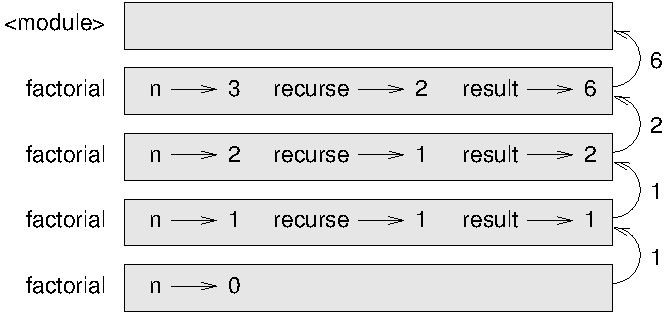
\includegraphics[scale=0.8]{figs/stack3.pdf}}
\caption{Διάγραμμα Στοίβας.}
\label{fig.stack3}
\end{figure}

\gr
Οι επιστρεφόμενες τιμές εμφανίζονται να περνάνε προς τα πίσω στη στοίβα.
Σε κάθε πλαίσιο, η επιστρεφόμενη τιμή είναι η τιμή της \en {\tt result}, \gr
η οποία είναι το γινόμενο της \en {\tt n} \gr και της \en {\tt recurse}.
\index{function frame} \index{frame}
\gr

Στο τελευταίο πλαίσιο, οι τοπικές μεταβλητές \en
{\tt recurse} \gr και \en {\tt result} \gr δεν υπάρχουν, γιατί
ο κλάδος που τις δημιουργεί δεν εκτελείται.


\section{Άλμα πίστης}
\index{recursion}
\index{leap of faith}

Ένας τρόπος να διαβάζουμε προγράμματα είναι να ακολουθούμε τη ροή εκτέλεσης,
κάτι το οποίο μπορεί να γίνει γρήγορα λαβύρινθος. Ένας εναλλακτικός τρόπος
είναι αυτό που εγώ ονομάζω \en "\gr άλμα πίστης\en " (leap of faith). \gr
Όταν βρεθείτε σε μία κλήση συνάρτησης, αντί να ακολουθήσετε τη ροή της εκτέλεσης,
υποθέστε ότι η συνάρτηση δουλεύει σωστά και επιστρέφει το σωστό αποτέλεσμα.

Στην πραγματικότητα, εφαρμόζετε ήδη αυτό το άλμα πίστης όταν χρησιμοποιείτε
τις ενσωματωμένες συναρτήσεις. Όταν καλείτε την \en {\tt math.cos} \gr ή \en
{\tt math.exp}, \gr δεν εξετάζετε τα σώματα αυτών των συναρτήσεων. Απλώς
θεωρείτε ότι δουλεύουν επειδή οι άνθρωποι που γράψανε τις ενσωματωμένες
συναρτήσεις ήταν καλοί προγραμματιστές.

Το ίδιο ισχύει και όταν καλείτε μία από τις δικές σας συναρτήσεις. Για
παράδειγμα, στην Ενότητα\en ~\ref{boolean}, \gr γράψαμε μία συνάρτηση με
όνομα \en \verb"is_divisible" \gr η οποία προσδιορίζει εάν ένας αριθμός
διαιρείται από έναν άλλο. Από τη στιγμή που πειστήκαμε ότι αυτή η συνάρτηση
είναι σωστή, εξετάζοντας και δοκιμάζοντας τον κώδικα, μπορούμε να χρησιμοποιήσουμε
τη συνάρτηση χωρίς να ξανακοιτάξουμε το σώμα της.
\index{testing!leap of faith}

Το ίδιο ισχύει και για τα αναδρομικά προγράμματα. Όταν βρεθείτε σε μία
αναδρομική κλήση, αντί να ακολουθήσετε τη ροή της εκτέλεσης,
θεωρήστε ότι η αναδρομική κλήση δουλεύει (παράγει το σωστό αποτέλεσμα)
και στη συνέχεια αναρωτηθείτε, \en "\gr Θεωρώντας ότι μπορώ να βρω το παραγοντικό
του \en $n-1$, \gr μπορώ να υπολογίσω το παραγοντικό του \en $n$ ; \gr Σε αυτή την
περίπτωση, είναι ξεκάθαρο ότι μπορείτε, πολλαπλασιάζοντας με \en $n$.\gr

Φυσικά, είναι λίγο περίεργο να θεωρούμε ότι η συνάρτηση δουλεύει σωστά
από τη στιγμή που δεν έχουμε τελειώσει το γράψιμό της, αλλά για αυτό
ονομάζεται άλμα πίστης\en !\gr


\section{Ένα ακόμα παράδειγμα}\en
\label{one.more.example}\gr

\index{fibonacci function}
\index{function!fibonacci}
Το επόμενο σύνηθες παράδειγμα, μετά το παραγοντικό, αναδρομικά οριζόμενης
μαθηματικής συνάρτησης είναι το \en {\tt fibonacci}, \gr του οποίου ο ορισμός
είναι \en (\gr βλ. \en \url{http://en.wikipedia.org/wiki/Fibonacci_number}):
%
\begin{eqnarray*}
&& \mathrm{fibonacci}(0) = 0 \\
&& \mathrm{fibonacci}(1) = 1 \\
&& \mathrm{fibonacci}(n) = \mathrm{fibonacci}(n-1) + \mathrm{fibonacci}(n-2)
\end{eqnarray*}
%
\gr
Γραμμένο σε \en Python, \gr μοιάζει κάπως έτσι\en :

\begin{verbatim}
def fibonacci (n):
    if n == 0:
        return 0
    elif  n == 1:
        return 1
    else:
        return fibonacci(n-1) + fibonacci(n-2)
\end{verbatim}
%
\gr
Αν προσπαθήσετε να ακολουθήσετε τη ροή της εκτέλεσης εδώ, ακόμα και
για αρκετά μικρές τιμές του \en $n$, \gr το κεφάλι σας θα εκραγεί.
Αλλά σύμφωνα με το άλμα πίστης, εάν υποθέσετε ότι οι δύο αναδρομικές
κλήσεις δουλεύουν σωστά, τότε είναι σαφές ότι αν τις προσθέσετε θα
πάρετε το σωστό αποτέλεσμα.
\index{flow of execution}


\section{Έλεγχος τύπων}
\label{guardian}

Τι θα συμβεί αν καλέσουμε την \en {\tt factorial} \gr και της δώσουμε σαν
όρισμα \en 1.5 ;
\index{type checking}
\index{error checking}
\index{factorial function}
\index{RuntimeError}

\begin{verbatim}
>>> factorial(1.5)
RuntimeError: Maximum recursion depth exceeded
\end{verbatim}
%
\gr
Μοιάζει με μία άπειρη αναδρομή. Αλλά πως γίνεται αυτό αφού υπάρχει μία
περίπτωση βάσης, όταν \en {\tt n == 0}. \gr Αλλά αν το \en {\tt n} \gr δεν
είναι ένας ακέραιος, μπορεί να \en "\gr χάσουμε\en "\gr την περίπτωση βάσης
και να έχουμε αναδρομή επ' άπειρον.
\index{infinite recursion}
\index{recursion!infinite}

Στην πρώτη αναδρομική κλήση, η τιμή του \en {\tt n} \gr είναι \en
0.5. \gr Στην επόμενη, είναι \en -0.5. \gr Και από εκεί και πέρα,
γίνεται όλο και μικρότερη (πιο αρνητική), αλλά ποτέ δεν θα γίνει 0.

Έχουμε δύο επιλογές. Μπορούμε να γενικεύσουμε την συνάρτηση \en
{\tt factorial} \gr για να δουλεύει και με αριθμούς κινητής υποδιαστολής,
ή να την μετατρέψουμε ούτως ώστε να ελέγχει τον τύπο του ορίσματός της.
Η πρώτη επιλογή ονομάζεται συνάρτηση γάμμα και είναι εκτός του σκοπού
αυτού του βιβλίου. Επομένως θα πάμε στη δεύτερη επιλογή.
\index{gamma function}

Μπορούμε να χρησιμοποιήσουμε την ενσωματωμένη συνάρτηση \en {\tt isinstance} \gr
για να επαληθέυσουμε τον τύπο του ορίσματος. Αφού το κάνουμε αυτό, μπορούμε επίσης να
σιγουρευτούμε ότι το όρισμα είναι θετικό\en :
\index{isinstance function}
\index{function!isinstance}

\begin{verbatim}
def factorial (n):
    if not isinstance(n, int):
        print 'Factorial is only defined for integers.'
        return None
    elif n < 0:
        print 'Factorial is not defined for negative integers.'
        return None
    elif n == 0:
        return 1
    else:
        return n * factorial(n-1)
\end{verbatim}
%
\gr
Η πρώτη περίπτωση βάσης χειρίζεται τους μη-ακέραιους και η δεύτερη \en
"\gr συλλαμβάνει\en " \gr τους αρνητικούς ακέραιους. Και στις δύο περιπτώσεις,
το πρόγραμμα εμφανίζει ένα μήνυμα λάθους και επιστρέφει \en {\tt None} \gr για να
υποδηλώσει ότι κάτι πήγε στραβά\en :

\begin{verbatim}
>>> factorial('fred')
Factorial is only defined for integers.
None
>>> factorial(-2)
Factorial is not defined for negative integers.
None
\end{verbatim}
%
\gr
Εάν περάσουμε και τους δύο ελέγχους, τότε ξέρουμε ότι το \en $n$ \gr
είναι θετικός ή μηδέν, και άρα μπορούμε να αποδείξουμε ότι η αναδρομή
τερματίζει.
\index{guardian pattern}
\index{pattern!guardian}

Αυτό το πρόγραμμα επιδεικνύει ένα πρότυπο το οποίο μερικές φορές ονομάζεται
\en "\gr φύλακας\en ". \gr Οι πρώτες δύο συνθήκες λειτουργούν σαν φύλακες,
προστατεύοντας τον κώδικα που ακολουθεί από τιμές οι οποίες μπορεί να προκαλέσουν
σφάλμα. Οι φύλακες καθιστούν δυνατή την αποδειξη της ορθότητας του κώδικα.

Στην ενότητα\en ~\ref{raise} \gr θα δούμε μία πιο ευέλικτη εναλλακτική λύση
για να εμφανίζουμε ένα μήνυμα λάθους εγείροντας μία εξαίρεση.


\section{Αποσφαλμάτωση}
\label{factdebug}

Σπάζοντας ένα μεγάλο πρόγραμμα σε μικρότερες συναρτήσεις δημιουργούνται
φυσικά σημεία ελέγχου για αποσφαλμάτωση. \index{debugging}
Αν μία συνάρτηση δε δουλεύει, τότε πρέπει να εξετάσετε τρία ενδεχόμενα\en :

\begin{itemize}

\item \gr Κάτι πήγε στραβά με τα ορίσματα που παίρνει η συνάρτηση.
Δηλαδή, μία προϋπόθεση παραβιάστηκε.\en

\item \gr Υπάρχει κάποιο λάθος στη συνάρτηση. Δηλαδή, μία μετασυνθήκη
παραβιάστηκε.\en

\item \gr Κάτι είναι λάθος με την επιστρεφόμενη τιμή ή με τον τρόπο
που χρησιμοποιήθηκε.\en

\end{itemize}
\gr
Για να αποκλείσετε το πρώτο εδεχόμενο, μπορείτε να προσθέσετε μία δήλωση
\en {\tt print} \gr στην αρχή της συνάρτησης και να εμφανίσετε τις τιμές των
παραμέτρων (και τους τύπους τους). Ή μπορείτε να γράψετε κώδικα ο οποίος θα
ελέγχει ρητά τις προϋποθέσεις.
\index{precondition}
\index{postcondition}

Εάν οι παράμετροι φαίνονται εντάξει, προσθέστε μία δήλωση \en {\tt print}
\gr πριν από κάθε δήλωση \en {\tt return} \gr η οποία θα εμφανίζει την
επιστρεφόμενη τιμή. Εάν είναι εφικτό, ελέγξτε το αποτέλεσμα με το χέρι.
Δοκιμάστε να καλέσετε τη συνάρτηση με τιμές που κάνουν εύκολο τον έλεγχο
του αποτελέσματος \en (\gr όπως στην Ενότητα\en ~\ref{incremental.development}).\gr

Αν φαίνεται ότι η συνάρτηση δουλεύει, εξετάστε την κλήση συνάρτησης
για να σιγουρευτείτε ότι η τιμή που επιστράφηκε χρησιμοποιείται σωστά
\en (\gr ή αν χρησιμοποιείτε γενικά\en !)\gr
\index{flow of execution}

Προσθέτοντας δηλώσεις \en {\tt print} \gr στην αρχή και στο τέλος μίας
συνάρτησης μπορεί να βοηθήσει να γίνει η ροή εκτέλεσης πιο ορατή.
Για παράδειγμα, αυτή είναι μία έκδοση της \en {\tt factorial} \gr με
δηλώσεις \en {\tt print}:

\begin{verbatim}
def factorial(n):
    space = ' ' * (4 * n)
    print space, 'factorial', n
    if n == 0:
        print space, 'returning 1'
        return 1
    else:
        recurse = factorial(n-1)
        result = n * recurse
        print space, 'returning', result
        return result
\end{verbatim}
%
\gr
Το \en {\tt space} \gr είναι μία συμβολοσειρά από κενούς χαρακτήρες για τη
ρύθμιση των εσοχών της εξόδου. Αυτό είναι το αποτέλεσμα της \en {\tt factorial(5)} :

\begin{verbatim}
                     factorial 5
                 factorial 4
             factorial 3
         factorial 2
     factorial 1
 factorial 0
 returning 1
     returning 1
         returning 2
             returning 6
                 returning 24
                     returning 120
\end{verbatim}
%
\gr
Αν είστε μπερδεμένοι με την ροή της εκτέλεσης, αυτού του είδους η έξοδος
μπορεί να είναι χρήσιμη. Χρειάζεται κάποιο χρόνο για να αναπτυχθεί μία \en
"\gr σκαλωσιά\en ", \gr αλλά λίγη σκαλωσιά μπορεί να μας γλιτώσει από πολύ
αποσφαλμάτωση.


\section{Ορολογία}

\begin{description}

\item[προσωρινή μεταβλητή:]  Μία μεταβλητή η οποία χρησιμοποιείτε για να
αποθηκεύεται μία ενδιάμεση τιμή σε έναν σύνθετο υπολογισμό.
\index{temporary variable}
\index{variable!temporary}

\item[νεκρός κώδικας:]  Μέρος του κώδικα το οποίο δεν μπορεί να εκτελεστεί ποτέ,
επειδή συνήθως εμφανίζεται μετά από μία δήλωση \en {\tt return}.
\index{dead code}

\item[{\tt None}:]  \gr Μία ειδική τιμή η οποία επιστρέφεται από συναρτήσεις οι
οποίες δεν έχουν καθόλου δήλωση επιστροφής ή έχουν δήλωση επιστροφής αλλά χωρίς
κανένα όρισμα.
\index{None special value}
\index{special value!None}

\item[σταδιακή ανάπτυξη:]  Ένα πλάνο ανάπτυξης προγραμμάτων που στοχεύει στην
αποφυγή της αποσφαλμάτωσης προσθέτοντας και δοκιμάζοντας μικρά κομμάτια
κώδικα κάθε φορά.
\index{incremental development}

\item[σκαλωσιά:]  Κώδικας ο οποίος χρησιμοποιείται κατά την ανάπτυξη ενός
προγράμματος αλλά δεν είναι μέρος της τελικής έκδοσης.
\index{scaffolding}

\item[φύλακας:]  Ένα προγραμματιστικό πρότυπο το οποίο χρησιμοποιεί δηλώσεις
υπό συνθήκη για να ελέγξει και να διαχειριστεί περιπτώσεις οι οποίες μπορεί
να προκαλέσουν κάποιο σφάλμα.
\index{guardian pattern}
\index{pattern!guardian}

\end{description}


\section{Ασκήσεις}

ΑΣΚΗΣΗ 6.4

Σχεδιάστε ένα διάγραμμα στοίβας για το ακόλουθο πρόγραμμα. Τι εμφανίζει το
πρόγραμμα\en ;
\gr
Λύση\en : \url{http://thinkpython.com/code/stack_diagram.py}.
\index{stack diagram}

\begin{verbatim}
def b(z):
    prod = a(z, z)
    print z, prod
    return prod

def a(x, y):
    x = x + 1
    return x * y

def c(x, y, z):
    total = x + y + z
    square = b(total)**2
    return square

x = 1
y = x + 1
print c(x, y+3, x+y)
\end{verbatim}


\gr
ΑΣΚΗΣΗ 6.5
\label{ackermann}

Η συνάρτηση Άκερμαν, $A(m, n)$, ορίζεται\en :

\begin{eqnarray*}
A(m, n) = \begin{cases}
              n+1 & \mbox{if } m = 0 \\
        A(m-1, 1) & \mbox{if } m > 0 \mbox{ and } n = 0 \\
A(m-1, A(m, n-1)) & \mbox{if } m > 0 \mbox{ and } n > 0.
\end{cases}
\end{eqnarray*}
%
\gr
Βλ. \en \url{http://en.wikipedia.org/wiki/Ackermann_function}. \gr
Γράψτε μία συνάρτηση με όνομα \en {\tt ack} \gr υπολογίζει τη
συνάρτηση του Άκερμαν. Χρησιμοποιήστε τη συνάρτησή σας για να
υπολογίσετε το \en {\tt ack(3, 4)}, \gr το οποίο θα πρέπει να βγεί 125.
Τι συμβαίνει για μεγαλύτερες τιμές του \en {\tt m} \gr και του \en {\tt n}; \gr
Λύση\en : \url{http://thinkpython.com/code/ackermann.py}.
\index{Ackermann function}
\index{function!ack}


\gr
ΑΣΚΗΣΗ 6.6
\label{palindrome}

Παλίνδρομο είναι μία λέξη η οποία συλλαβίζεται το ίδιο προς τα πίσω
και προς τα εμπρός, όπως είναι η \en ``noon'' \gr και η \en ``redivider''. \gr
Αναδρομικά, μία λέξη είναι παλίνδρομο αν το πρώτο και το τελευταίο γράμμα είναι
ίδια και τα μεσαία είναι παλίνδρομο.
\index{palindrome}

Οι ακόλουθες, είναι συναρτήσεις οι οποίες παίρνουν μία συμβολοσειρά
σαν όρισμα και επιστρέφουν το πρώτο, το τελευταίο και τα μεσαία γράμματα\en :

\begin{verbatim}
def first(word):
    return word[0]

def last(word):
    return word[-1]

def middle(word):
    return word[1:-1]
\end{verbatim}
%
\gr
Θα δούμε πως δουλεύουν στο Κεφάλαιο\en ~\ref{strings}.\gr

\begin{enumerate}

\item Πληκτρολογήστε αυτές τις συναρτήσεις μέσα σε ένα αρχείο
με όνομα \en {\tt palindrome.py} \gr και δοκιμάστε τες. Τι συμβαίνει
αν καλέσετε τη \en {\tt middle} \gr με μία συμβολοσειρά με δύο γράμματα\en ; \gr
Μέ ένα γράμμα\en ; \gr Τι γίνεται με μία κενή συμβολοσειρα, η οποία
γράφεται έτσι \en \verb"''" \gr και δεν περιέχει καθόλου γράμματα\en ;\gr

\item Γράψτε μία συνάρτηση με όνομα \en \verb"is_palindrome" \gr
η οποία θα παίρνει σαν όρισμα μία συμβολοσειρά και θα επιστρέφει \en
{\tt True} \gr εάν είναι παλίνδρομο και \en {\tt False} \gr αλλιώς.
Θυμηθείτε ότι μπορείτε να χρησιμοποιήσετε την ενσωματωμένη συνάρτηση
\en {\tt len} \gr για να ελέγξετε το μήκος μίας συμβολοσειράς.

\end{enumerate}

Λύση\en : \url{http://thinkpython.com/code/palindrome_soln.py}.\gr


ΑΣΚΗΣΗ 6.7

Ένας αριθμός \en $a$, \gr είναι μία δύναμη του \en $b$ \gr εάν
διαιρείται από το \en $b$ \gr και το \en $a/b$ \gr είναι μία δύναμη
του \en $b$. \gr Γράψτε μία συνάρτηση με όνομα \en \verb"is_power" \gr
η οποία θα παίρνει σαν παραμέτρους το \en {\tt a} \gr και το \en {\tt b} \gr
και θα επιστρέφει \en {\tt True} \gr αν το \en {\tt a} \gr είναι μία
δύναμη του \en {\tt b}. \gr
Σημείωση\en : \gr θα πρέπει να σκεφτείτε την περίπτωση βάσης.



ΑΣΚΗΣΗ 6.8
\index{greatest common divisor (GCD)}
\index{GCD (greatest common divisor)}

Ο μέγιστος κοινός διαιρέτης \en (GCD) \gr του \en $a$ \gr και του \en $b$ \gr
είναι ο μεγαλύτερος αριθμός που διαιρεί και τους δύο χώρις να αφήνει υπόλοιπο.

Ένας τρόπος για να βρούμε τον \en GCD \gr δύο αριθμών είναι ο
αλγόριθμος του Ευκλείδη, ο οποίος βασίζεται παρατήρηση ότι αν
το \en $r$ \gr είναι το υπόλοιπο όταν το \en $a$ \gr διαιρείται από
το \en $b$, \gr τότε \en $gcd(a, b) = gcd(b, r)$. \gr
Σαν περίπτωση βάσης, μπορούμε να χρησιμοποιήσουμε την \en
$gcd(a, 0) = a$.\gr
\index{Euclid's algorithm}
\index{algorithm!Euclid}

Γράψτε μία συνάρτηση με όνομα \en \verb"gcd" \gr η οποία παίρνει
σαν παραμέτρους το \en {\tt a} \gr και το \en {\tt b} \gr και θα
επιστρέφει τον μέγιστο κοινό διαιρέτη τους. Αν χρειαστείτε βοήθεια,
δείτε εδώ\en : \url{http://en.wikipedia.org/wiki/Euclidean_algorithm}.

\gr
Αναφορά\en : \gr Αυτή η άσκηση βασίζεται σε ένα παράδειγμα του
βιβλίου \en {\em Structure and Interpretation of Computer Programs} \gr
των Άμπελσον και Σούσμαν.



\chapter{Επανάληψη}

\section{Πολλαπλή εκχώρηση}
\index{assignment}
\index{statement!assignment}
\index{multiple assignment}

Ίσως να έχετε ανακαλύψει, ότι είναι έγκυρο να κάνουμε περισσότερες
από μία εκχωρήσεις στην ίδια μεταβλητή. Μία νέα εκχώρηση κάνει μία μεταβλητή
να αναφέρεται σε μία νέα τιμή (και παύει η αναφορά στην παλιά τιμή). \en

\begin{verbatim}
bruce = 5
print bruce,
bruce = 7
print bruce
\end{verbatim}
%
\gr
Η έξοδος αυτού του προγράμματος είναι \en {\tt 5 7}, \gr επειδή τη
πρώτη φορά που τυπώνεται η \en {\tt bruce} \gr η τιμή της είναι 5,
ενώ τη δεύτερη φορά η τιμή της είναι 7. Το κόμμα στο τέλος της πρώτης
δήλωσης \en {\tt print} \gr καταστέλλει τη νέα γραμμή, γι' αυτό και
οι δύο έξοδοι εμφανίζονται στην ίδια γραμμή.
\index{newline}

Η εικόνα\en ~\ref{fig.assign2} \gr δείχνει πως φαίνεται η πολλαπλή
εκχώρηση σε ένα διάγραμμα κατάστασης.
\index{state diagram} \index{diagram!state}

Είναι ιδιαίτερα σημαντικό, στην πολλαπλή εκχώρηση, να γίνει διάκριση
μεταξύ μίας εκχώρησης τιμής και μίας δήλωσης ισότητας. Επειδή η \en
Python \gr χρησιμοποιεί το σύμβολο της ισότητας \en ({\tt =}) \gr για
εκχώρηση, είναι σύνηθες φαινόμενο να ερμηνεύουμε μία τέτοια δήλωση \en {\tt a = b} \gr
σαν μία δήλωση ισότητας. Αλλά δεν είναι\en !\gr
\index{equality and assignment}

Πρώτον, η ισότητα είναι μία συμμετρική σχέση ενώ η εκχώρηση όχι. Για
παράδειγμα, στα μαθηματικά, εάν \en $a=7$ \gr τότε και \en $7=a$. \gr
Αλλά στην \en Python, \gr ενώ η δήλωση \en {\tt a = 7} \gr είναι έγκυρη,
η \en {\tt 7 = a} \gr δεν είναι.

Επί πλέον, στα μαθηματικά, μία δήλωση ισότητας είναι είτε αληθής είτε
ψευδής για πάντα. Αν \en $a=b$ \gr τώρα, τότε το \en $a$ \gr θα είναι
πάντα ίσο με το \en $b$. \gr Στην \en Python, \gr μία δήλωση εκχώρησης
μπορεί να κάνει δύο μεταβλητές ίσες, αλλά δεν είναι απαραίτητο να μείνουν
έτσι\en :

\begin{verbatim}
a = 5
b = a    # a and b are now equal
a = 3    # a and b are no longer equal
\end{verbatim}
%
\gr
Η τρίτη γραμμή αλλάζει την τιμή της \en {\tt a} \gr αλλά δεν αλλάζει
την τιμή της \en {\tt b}, \gr και επομένως δεν είναι πλέον ίσες.

Παρόλο που η πολλαπλή εκχώρηση είναι συχνά χρήσιμη, θα πρέπει να τη
χρησιμοποιείτε με προσοχή. Αν οι τιμές των μεταβλητών αλλάζουν συχνά,
μπορεί να κάνει την ανάγνωση και την αποσφαλμάτωση του κώδικα δύσκολη.

\begin{figure}
\centerline
{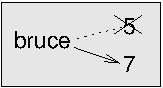
\includegraphics[scale=0.8]{figs/assign2.pdf}}
\caption{Διάγραμμα κατάστασης.}
\label{fig.assign2}
\end{figure}


\section{Ενημέρωση μεταβλητών}
\label{update}

\index{update}
\index{variable!updating}

Μία από τις συχνότερες μορφές της πολλαπλής εκχώρησης είναι η ενημέρωση,
όπου η νέα τιμή της μεταβλητής εξαρτάται από την παλία.\en

\begin{verbatim}
x = x+1
\end{verbatim}
%
\gr
Αυτό σημαίνει\en : "\gr πάρε την τιμή του \en {\tt x}, \gr πρόσθεσε ένα και
μετά ενημέρωσε το \en {\tt x} \gr με τη νέα τιμή\en ".\gr

Αν προσπαθήσετε να ενημερώσετε μία μεταβλητή η οποία δεν υπάρχει, θα πάρετε
μήνυμα λάθους, επειδή η \en Python \gr υπολογίζει πρώτα το δεξιό μέρος πριν
εκχωρήσει μία τιμή στο \en {\tt x}:

\begin{verbatim}
>>> x = x+1
NameError: name 'x' is not defined
\end{verbatim}
%
\gr
Για να είστε σε θέση να ενημερώσετε μία μεταβλητή, πρέπει πρώτα να την
αρχικοποιήσετε, συνήθως με μία απλή εκχώρηση\en :
\index{initialization (before update)}

\begin{verbatim}
>>> x = 0
>>> x = x+1
\end{verbatim}
%
\gr
Η ενημέρωση μίας μεταβλητής προσθέτοντας της 1 ονομάζεται προσαύξηση,
ενώ αφαιρώντας 1 ονομάζεται μείωση μεταβλητής.\en
\index{increment}
\index{decrement}




\section{$\Delta\eta\lambda\omega\sigma\eta$ \tt while}
\index{statement!while}
\index{while loop}
\index{loop!while}
\index{iteration}

\gr
Οι υπολογιστές χρησιμοποιούνται συχνά για την αυτοματοποίηση επαναλαμβανόμενων
εργασιών. Η επανάληψη πανομοιότυπων ή παρόμοιων εργασιών χώρις λάθη είναι μία
εύκολη υπόθεση για τους υπολογιστές αλλά όχι και για τους ανθρώπους.

Έχουμε δει δύο προγράμματα, το \en {\tt countdown} \gr και το \en \verb"print_n", \gr
τα οποία χρησιμοποιούν αναδρομή για να εκτελέσουν επανάληψη. Επειδή η επανάληψη
χρησιμοποιείται συχνά, η \en Python \gr παρέχει διάφορες δυνατότητες για να την
κάνει ευκολότερη. Η μία είναι η δήλωση \en {\tt for} \gr που είδαμε στην Ενότητα~\ref{repetition}.
Θα επανέλθουμε σε αυτήν αργότερα.

Μία άλλη είναι η δήλωση \en {\tt while}. \gr Αυτή είναι μία έκδοση
της \en {\tt countdown} \gr η οποία χρησιμοποιεί μία δήλωση \en {\tt while}:

\begin{verbatim}
def countdown(n):
    while n > 0:
        print n
        n = n-1
    print 'Blastoff!'
\end{verbatim}
%
\gr
Η δήλωση \en {\tt while} \gr διαβάζεται σχεδόν σαν να μία πρόταση στα Αγγλικά.
Αυτό σημαίνει ότι\en : ''\gr Όσο το \en {\tt n} \gr είναι μεγαλύτερο του 0,
εμφάνισε την τιμή του \en {\tt n} \gr και στη συνάχεια μείωσε την τιμή του κατά 1.
Όταν φτάσεις στο 0, εμφάνισε τη λέξη \en {\tt Blastoff}''!\gr
\index{flow of execution}

Πιο επίσημα, αυτή είναι η ροή εκτέλεσης για μία δήλωση \en {\tt while}:
\gr
\begin{enumerate}

\item Αξιολόγησε τη συνθήκη, επέστρεψε \en {\tt True} \gr ή \en {\tt False}.\gr

\item Αν η συνθήκη είναι ψευδής, βγες από τη δήλωση \en {\tt while} \gr και συνέχισε με την εκτέλεση της επόμενης δήλωσης.

\item Αν η συνθήκη είναι αληθής, εκτέλεσε το σώμα και μετά επέστρεψε στο πρώτο βήμα.

\end{enumerate}

Αυτος ο τύπος ροής ονομάζεται βρόχος \en ({\bf loop}) \gr επειδή το
τρίτο βήμα επιστρέφει τη ροή στην αρχή.
\index{condition}
\index{loop}
\index{body}

Το σώμα του βρόγχου θα πρέπει να αλλάζει την τιμή ενός ή περισσοτέρων
μεταβλητών έτσι ώστε τελικά η συνθήκη να γίνει ψευδής και να τερματίσει
ο βρόγχος, αλλιώς ο βρόγχος θα επαναλαμβάνεται επ' απειρον. Ένας τέτοιος βρόγχος ονομάζεται
ατέρμων βρόγχος. Μία ατέλειωτη πηγή διασκέδασης για τους επιστήμονες της
πληροφορικής είναι η παρατήρηση ότι οι οδηγίες για ένα σαμπουάν, \en "\gr
Σαπουνίστε, ξεπλύνετε, επαναλάβετε,\en " \gr αποτελούν έναν ατέρμων βρόγχο.
\index{infinite loop}
\index{loop!infinite}

Στην περίπτωση της \en {\tt countdown}, \gr μπορούμε να αποδείξουμε ότι ο
βρόγχος τερματίζει επειδή ξέρουμε ότι η τιμή του \en {\tt n} \gr είναι πεπερασμένη,
και μπορούμε να δούμε ότι η τιμή του μειώνεται σε κάθε επανάληψη του βρόγχου, έτσι
ώστε τελικά να πάρει την τιμή 0. Σε άλλες περιπτώσεις όμως δεν είναι τόσο εύκολο\en :

\begin{verbatim}
def sequence(n):
    while n != 1:
        print n,
        if n%2 == 0:        # n is even
            n = n/2
        else:               # n is odd
            n = n*3+1
\end{verbatim}
%
\gr
Η συνθήκη για αυτό το βρόγχο είναι η \en {\tt n != 1}, \gr άρα ο βρόγχος
συνεχίζει να εκτελείται μέχρι το \en {\tt n} \gr να γίνει \en {\tt 1}, \gr
το οποίο κάνει τη συνθήκη ψευδή.

Σε κάθε επανάληψη, το πρόγραμμα εμφανίζει την τιμή του \en {\tt n} \gr
και ελέγχει εάν είναι άρτιος ή περιττός. Αν είναι άρτιος, το \en {\tt n} \gr
διαιρείται με το 2. Αν είναι περιττός, η τιμή του \en {\tt n} \gr αντικαθιστάται
με \en {\tt n*3+1}. \gr Για παράδειγμα, αν περάσουμε το 3 σαν όρισμα στην \en
{\tt sequence}, \gr η σειρά των αποτελεσμάτων θα είναι\en : 3, 10, 5, 16, 8, 4, 2, 1.\gr

Από τη στιγμή που το \en {\tt n} \gr άλλες φορές αυξάνεται και άλλες φορές
μειώνεται, δεν υπάρχει κάποια προφανής απόδειξη ότι το \en {\tt n} \gr θα γίνει
ποτέ ίσο με 1, ή ότι το πρόγραμμα τερματίζει. Για κάποιες συγκεκριμένες τιμές του \en
{\tt n}, \gr μπορούμε να αποδέιξουμε τον τερματισμό του προγράμματος. Για παράδειγμα,
αν η αρχική τιμή του \en {\tt n} \gr είναι μία δύναμη του δύο, τότε η τιμή του \en {\tt n} \gr
σε κάθε επανάληψη θα είναι άρτια μέχρι να γίνει ίση με 1. Το προηγούμενο παράδειγμα τελειώνει
με μία τέτοια ακολουθία, ξεκινώντας με 16.
\index{Collatz conjecture}

Το δύσκολο είναι να αποδέιξουμε ότι το πρόγραμμα τερματίζει για οποιαδήποτε
θετική τιμή του \en {\tt n}. \gr Μέχρι στιγμής, κανείς δεν μπόρεσε να το αποδείξει ή
να το διαψέυσει\en ! (\gr Βλ. \en \url{http://en.wikipedia.org/wiki/Collatz_conjecture}).\gr

ΑΣΚΗΣΗ 7.1.

Ξαναγράψτε τη συνάρτηση \en \verb"print_n" \gr της ενότητας\en ~\ref{recursion} \gr
χρησιμοποιώντας επανάληψη αντί για αναδρομή.\en



\section{{\tt break}}
\index{break statement}
\index{statement!break}

\gr
Μερικές φορές δεν ξέρετε ότι ήρθε η ώρα για να τελειώσει ένας βρόγχος μέχρι να
φτάσετε στη μέση του σώματός του. Σε αυτήν την περίπτωση μπορείτε να χρησιμοποιήσετε
τη δήλωση \en {\tt break} \gr για να βγείτε έξω από το βρόγχο.

Για παράδειγμα, υποθέστε ότι θέλετε να δέχεστε είσοδο από το χρήστη μέχρις ότου
πληκτρολογήσει \en {\tt done}. \gr Μπορείτε να γράψετε\en :

\begin{verbatim}
while True:
    line = raw_input('> ')
    if line == 'done':
        break
    print line

print 'Done!'
\end{verbatim}
%
\gr
Η συνθήκη τερματισμού του βρόγχου είναι η \en {\tt True}, \gr η οποία είναι
πάντα αληθής, και άρα ο βρόγχος εκτελείται μέχρι να φτάσει στην δήλωση \en break.\gr

Σε κάθε επανάληψη, ζητάει είσοδο από το χρήστη με το σύμβολο \en '>'.\gr
Αν ο χρήστης πληκτρολογήσει \en {\tt done}, \gr τότε βγαίνει από το βρόγχο με τη δήλωση
\en {\tt break}. \gr Αλλιώς, το πρόγραμμα εμφανίζει ότι πληκτρολογεί ο χρήστης και
επιστρέφει στην αρχή του βρόγχου. Αυτό είναι ένα δείγμα εκτέλεσης\en :

\begin{verbatim}
> not done
not done
> done
Done!
\end{verbatim}
%
\gr
Αυτός ο τρόπος γραφής \en {\tt while} \gr βρόγχων είναι πολύ κοινός
επειδή μπορείτε να ελέγξετε τη συνθήκη οπουδήποτε μέσα στο βρόγχο (όχι
μόνο στην αρχή) και επίσης μπορείτε να εκφράσετε τη συνθήκη τερματισμού
καταφατικά \en(\gr σταμάτα όταν συμβεί αυτό\en ) \gr αντί για αρνητικά \en
(\gr συνέχισε μέχρι να συμβεί αυτό\en ).\gr


\section{Τετραγωνικές ρίζες}
\label{squareroot}
\index{square root}

Οι βρόγχοι χρησιμοποιούνται συχνά σε προγράμματα τα οποία
υπολογίζουν αριθμητικά αποτελέσματα αρχίζοντας με μία κατά προσέγγιση
απάντηση την οποία βελτιώνουν σε κάθε επανάληψη.
\index{Newton's method}

Για παράδειγμα, ένας τρόπος υπολογισμού της τετραγωνικής ρίζας ενός αριθμού
είναι η μέθοδος του Νιούτον. Υποθέστε ότι θέλετε να υπολογίσετε την τετραγωνική ρίζα
του \en $a$. \gr Αν ξεκινήσετε με, σχεδόν, οποιαδήποτε εκτίμηση \en $x$, \gr τότε μπορείτε
να υπολογίσετε μία καλύτερη εκτίμηση με τον ακόλουθο τύπο\en :

\[ y = \frac{x + a/x}{2} \]
%
\gr
Για παράδειγμα, αν το \en $a$ \gr είναι 4 και το \en $x$ \gr είναι 3\en :

\begin{verbatim}
>>> a = 4.0
>>> x = 3.0
>>> y = (x + a/x) / 2
>>> print y
2.16666666667
\end{verbatim}
%
\gr
Το οποίο είναι πιο κοντά στη σωστή απάντηση \en ($\sqrt{4} = 2$). \gr Αν
επαναλάβουμε τη διαδικασία με τη νέα εκτίμηση, τότε πλησιάζουμε ακόμα περισσότερο\en :

\begin{verbatim}
>>> x = y
>>> y = (x + a/x) / 2
>>> print y
2.00641025641
\end{verbatim}
%
\gr
Μετά από μερικές ακόμα ενημερώσεις, η εκτίμηση είναι σχεδόν ακριβής\en :
\index{update}

\begin{verbatim}
>>> x = y
>>> y = (x + a/x) / 2
>>> print y
2.00001024003
>>> x = y
>>> y = (x + a/x) / 2
>>> print y
2.00000000003
\end{verbatim}
%
\gr
Σε γενικές γραμμές δεν γνωρίζουμε εκ των προτέρων πόσα βήματα θα χρειαστούμε
για να φτάσουμε στη σωστή απάντηση, αλλά ξέρουμε ότι φτάσαμε όταν η εκτίμηση
σταματήσει να αλλάζει\en :

\begin{verbatim}
>>> x = y
>>> y = (x + a/x) / 2
>>> print y
2.0
>>> x = y
>>> y = (x + a/x) / 2
>>> print y
2.0
\end{verbatim}
%
\gr
Όταν \en {\tt y == x}, \gr μπορούμε να σταματήσουμε. Ακολουθεί ένας βρόγχος ο
οποίος ξεκινάει με μία αρχική εκτίμηση, \en {\tt x}, \gr και τη βελτιώνει μέχρι
να σταματήσει να αλλάζει\en :

\begin{verbatim}
while True:
    print x
    y = (x + a/x) / 2
    if y == x:
        break
    x = y
\end{verbatim}
%
\gr
Για τις περισσότερες τιμές του \en {\tt a} \gr δουλεύει καλά, αλλά γενικά
είναι επίφοβο να ελέγχουμε την ισότητα δεκαδικών αριθμών. Οι τιμές των αριθμών
κινητής υποδιαστολής είναι σωστές μόνο κατά προσέγγιση. Οι περισσότεροι ρητοί
όπως το \en $1/3$ \gr και άρρητοι αριθμοί όπως η \en $\sqrt{2}$ \gr δεν μπορούν
να αναπαρασταθούν με ακρίβεια από ένα δεκαδικό αριθμό.
\index{floating-point}
\index{epsilon}

Αντί να ελέγχουμε αν το \en {\tt x} \gr και το \en {\tt y} \gr είναι ακριβώς ίσα,
είναι ασφαλέστερο να χρησιμοποιούμε την ενσωματωμένη συνάρτηση \en {\tt abs} \gr για
υπολογίσουμε την απόλυτη τιμή ή το μέγεθος της διαφοράς τους\en :

\begin{verbatim}
    if abs(y-x) < epsilon:
        break
\end{verbatim}
%
\gr
Όπου το \en \verb"epsilon" \gr έχει μία τιμή όπως η \en {\tt 0.0000001} \gr
η οποία καθορίζει πόσο κοντά είναι αρκετά κοντά.

ΑΣΚΗΣΗ 7.2.

Ενθυλακώστε αυτό το βρόγχο σε μία συνάρτηση με όνομα \en \verb"square_root" \gr
η οποία θα παίρνει το \en {\tt a} \gr σαν μία παράμετρο, θα διαλέγει μία λογική
τιμή του \en {\tt x} \gr και θα επιστρέφει μία εκτίμηση της τετραγωνικής ρίζας του
\en {\tt a}.\gr


\section{Αλγόριθμοι}
\index{algorithm}

Η μέθοδος του Νιούτον αποτελεί ένα παράδειγμα ενός αλγορίθμου\en : \gr
μία μηχανική διαδικασία για την επίλυση μίας κατηγορίας προβλημάτων \en
(\gr σε αυτήν την περίπτωση, ο υπολογισμός της τετραγωνικής ρίζας ενός αριθμού\en ).\gr

Δεν είναι εύκολο να οριστεί ένας αλγόριθμος. Θα σας βοηθούσε εάν ξεκινούσατε με κάτι
το οποίο δεν είναι αλγόριθμος. Όταν μάθατε να πολλάπλασιάζετε μονοψήφιους αριθμούς,
τότε μάλλον απομνημονεύσατε και την προπαίδεια. Και έτσι, απομνημονεύσατε 100 συγκεκριμένες
λύσεις. Αυτού του τύπου η γνώση δεν είναι αλγόριθμος.

Αλλά αν ήσασταν \en "\gr τεμπέληδες\en " \gr τότε μάλλον κλέψατε μαθαίνοντας μερικά κόλπα.
Για παράδειγμα, για να βρείτε το γινόμενο του \en $n$ \gr με το 9, μπορείτε να γράψετε \en
$n-1$ \gr για το πρώτο ψηφίο και \en $10-n$ \gr για το δεύτερο. Αυτό το κόλπο είναι μία
γενική λύση για τον πολλαπλασιασμό ενός οποιουδήποτε μονοψήφιου αριθμού με το 9. Αυτό είναι
ένας αλγόριθμος\en !\gr
\index{addition with carrying}
\index{carrying, addition with}
\index{subtraction!with borrowing}
\index{borrowing, subtraction with}

Ομοίως, οι τεχνικές που μάθατε για την πρόσθεση με κρατούμενο, την αφαίρεση με
δανεισμό και τη διαίρεση είναι όλες αλγόριθμοι. Ένα από τα χαρακτηριστικά των
αλγορίθμων είναι ότι δεν απαιτούν ευφυΐα για να εκτελεστούν. Είναι μηχανικές διαδικασίες
στις οποίες κάθε βήμα απορρέει από το προηγούμενο με βάση ένα απλό σύνολο κανόνων.

Κατά τη γνώμη μου, είναι πολύ δυσάρεστο το γεγονός ότι οι άνθρωποι ξοδεύουν τόσο πολύ
χρόνο στα σχολεία για να μάθουν να εκτελούν αλγόριθμους το οποίο, στην κυριολεξία, δεν
χρειάζεται καθόλου ευφυΐα.

Από την άλλη πλευρά, η διαδικασία του σχεδιασμού αλγορίθμων είναι μία ενδιαφέρουσα
πνευματική πρόκληση η οποία αποτελεί βασικό μέρος αυτού που ονομάζουμε προγραμματισμό.

Μερικά από τα πράγματα τα οποία οι άνθρωποι κάνουν φυσικά, χωρίς δυσκολία ή συνειδητή
σκέψη, είναι πολύ δύσκολο να εκφραστούν αλγοριθμικά. Ένα καλό παράδειγμα είναι η κατανόηση
μίας φυσικής γλώσσας. Αυτό το κάνουμε όλοι, αλλά μέχρι στιγμής κανένας δεν ήταν σε θέση να
εξηγήσει \en "\gr πως\en " \gr το κάνουμε, ή τουλάχιστον όχι με τη μορφή αλγόριθμου.


\section{Αποσφαλμάτωση}

Όσο θα γράφετε όλο και μεγαλύτερα προγράμματα, ίσως διαπιστώσετε ότι αφιερώνετε
περισσότερο χρόνο για αποσφαλμάτωση. Γράφοντας περισσότερο κώδικα αυξάνονται οι
πιθανότητες να κάνετε κάποιο λάθος μιας και υπάρχει περισσότερος χώρος για να
κρυφτούν τα σφάλματα.
\index{debugging!by bisection}
\index{bisection, debugging by}

Ένας τρόπος για να μειώσετε το χρόνο αποσφαλμάτωσης είναι η \en "\gr αποσφαλμάτωση με
διχοτόμηση\en ". \gr Για παράδειγμα, αν υπάρχουν 100 γραμμές στο πρόγραμμά σας και εσείς
τις ελέγξετε όλες μία μία, θα χρειαζόσασταν 100 βήματα.

Αντ' αυτού, δοκιμάστε να σπάσετε το πρόγραμμα στη μέση. Ψάξτε στη μέση του προγράμματος, ή
κάπου κοντά σε αυτήν, για μία ενδιάμεση τιμή την οποία μπορείτε να ελέγξετε. Προσθέστε μία
δήλωση \en {\tt print} \gr (ή κάτι άλλο το οποίο θα έχει επαληθεύσιμη επίδραση) και τρέξτε το
πρόγραμμα.

Εάν το αυτό το σημείο ελέγχου στη μέση είναι εσφαλμένο, τότε πρέπει να υπάρχει λάθος στο πρώτο
μισό του προγράμματος. Αν είναι σωστό, τότε το πρόβλημα είναι στο δεύτερο μισό.

Κάθε φορά που εκτελείτε έναν τέτοιο έλεγχο, μειώνετε κατά το ήμισυ τις γραμμές που πρέπει να
ψάξετε για να βρείτε το λάθος. Θεωρητικά, μετά από έξι βήματα (τα οποία είναι λιγότερα από 100)
θα είστε στη μία ή δύο γραμμές του κώδικα που βρίσκετε το λάθος.

Στην πράξη, δεν είναι πάντα ξεκάθαρο ποια είναι η \en "\gr μέση του προγράμματος\en " \gr και δεν
ίσως να μην είναι και δυνατόν να να τη βρούμε. Δεν έχει νόημα να μετράμε γραμμές για να βρούμε ακριβώς
το σημείο της μέσης. Αντ' αυτού, ψάξτε για περιοχές στο κώδικα που μπορεί να υπάρχουν λάθη και σημεία
που είναι εύκολο να βάλετε έναν έλεγχο. Και στη συνέχεια διαλέξτε ένα σημείο όπου οι πιθανότητες, για
το σφάλμα να είναι πριν ή μετά του σημείου ελέγχου, είναι περίπου ίδιες.




\section{Ορολογία}

\begin{description}

\item[πολλαπλή εκχώρηση:] Το να γίνονται περισσότερες από μία εκχωρήσεις τιμής στην ίδια μεταβλητή
κατά την εκτέλεση του προγράμματος.
\index{multiple assignment}
\index{assignment!multiple}

\item[ενημέρωση:] Μία εκχώρηση όπου η νέα τιμή της μεταβλητής εξαρτάται από την παλιά.
\index{update}

\item[αρχηκοποίηση:] Μία εκχώρηση η οποία δείνει αρχική τιμή σε μία μεταβλητή η οποία θα ενημερωθεί.
\index{initialization!variable}

\item[προσαύξηση:] Μία ενημέρωση η οποία αυξάνει την τιμή μίας μεταβλητής (συνήθως κατά ένα).
\index{increment}

\item[μείωση:] Μία ενημέρωση η οποία μειώνει την τιμή μίας μεταβλητής.
\index{decrement}

\item[επανάληψη:] Επαναλαμβανόμενη εκτέλεση ενός συνόλου δηλώσεων χρησιμοποιώντας είτε μία
αναδρομική συνάρτηση είτε έναν βρόγχο.
\index{iteration}

\item[ατέρμων βρόγχος:] Ένας βρόγχος στον οποίο η συνθήκη τέλους δεν ικανοποιείται ποτέ.
\index{infinite loop}

\end{description}


\section{Ασκήσεις}

ΑΣΚΗΣΗ 7.3.
\index{algorithm!square root}

Για να ελέγξετε τον αλγόριθμο υπολογισμού τετραγωνικής ρίζας αυτού του κεφαλαίου,
μπορείτε να το συγκρίνετε με τη \en {\tt math.sqrt}. \gr Γράψτε μία συνάρτηση με
όνομα \en \verb"test_square_root" \gr η οποία θα εμφανίζει στην οθόνη έναν τέτοιο
πίνακα\en :

\begin{verbatim}
1.0 1.0           1.0           0.0
2.0 1.41421356237 1.41421356237 2.22044604925e-16
3.0 1.73205080757 1.73205080757 0.0
4.0 2.0           2.0           0.0
5.0 2.2360679775  2.2360679775  0.0
6.0 2.44948974278 2.44948974278 0.0
7.0 2.64575131106 2.64575131106 0.0
8.0 2.82842712475 2.82842712475 4.4408920985e-16
9.0 3.0           3.0           0.0

\end{verbatim}
%
\gr
Η πρώτη στήλη είναι ένας αριθμός \en $a$, \gr η δεύτερη είναι η τετραγωνική
ρίζα του \en $a$ \gr υπολογισμένη με τη συνάρτηση από την Ενότητα\en ~\ref{squareroot}, \gr
η τρίτη στήλη είναι η τετραγωνική ρίζα υπολογισμένη από τη \en {\tt math.sqrt}, \gr και η
τέταρτη στήλη είναι η απόλυτη τιμή της διαφοράς μεταξύ των δύο υπολογισθέντων τιμών.


ΑΣΚΗΣΗ 7.4.
\index{eval function}
\index{function!eval}

Η ενσωματωμένη συνάρτηση \en {\tt eval} \gr παίρνει μία συμβολοσειρά σαν όρισμα και την
υπολογίζει χρησιμοποιώντας τον διερμηνέα της \en Python. \gr Για παράδειγμα\en :

\begin{verbatim}
>>> eval('1 + 2 * 3')
7
>>> import math
>>> eval('math.sqrt(5)')
2.2360679774997898
>>> eval('type(math.pi)')
<type 'float'>
\end{verbatim}
%
\gr
Γράψτε μία συνάρτηση με όνομα \en \verb"eval_loop" \gr η οποία προτρέπει
επαναληπτικά τον χρήστη, παίρνει την είσοδο και την υπολογίζει χρησιμοποιώντας
την \en {\tt eval} \gr και μετά εμφανίζει το αποτέλεσμα.

Θα πρέπει να συνεχίζει μέχρι ο χρήστης να πληκτρολογήσει \en \verb"'done'" \gr και
στη συνέχεια να επιστρέφει την τελευταία έκφραση που υπολόγισε.



ΑΣΚΗΣΗ 7.5.
\index{Ramanujan, Srinivasa}

Ο μαθηματικός Σρινιβάσα Ραμανούτζαν βρήκε μία άπειρη σειρά η οποία μπορεί να
χρησιμοποιηθεί για να παράγει μία αριθμιτική προσέγγιση του \en $\pi$ :
\index{pi}

\[ \frac{1}{\pi} = \frac{2\sqrt{2}}{9801}
\sum^\infty_{k=0} \frac{(4k)!(1103+26390k)}{(k!)^4 396^{4k}} \]

\gr
Γράψτε μία συνάρτηση με όνομα \en \verb"estimate_pi" \gr η οποία θα χρησιμοποιεί αυτόν
τον τύπο για να υπολογίσει και να επιστρέψει μία εκτίμηση του \en $\pi$. \gr Θα πρέπει
να χρησιμοποιεί έναν βρόγχο \en {\tt while} \gr για να υπολογίζει τους όρου της άθροισης
μέχρι ο τελευταίος όρος να είναι μικρότερος του \en {\tt 1e-15} \gr (ο οποίος είναι τρόπος
συμβολισμού του \en $10^{-15}$ \gr στην \en Python). \gr Μπορείτε να ελέγξετε το αποτέλεσμα
συγκρίνοντάς το με την \en {\tt math.pi}.\gr

Λύση\en : \url{http://thinkpython.com/code/pi.py}.\gr


\chapter{Συμβολοσειρές}
\label{strings}


\section{Μία συμβολοσειρά είναι μία ακολουθία}

\index{sequence}
\index{character}
\index{bracket operator}
\index{operator!bracket}
Μία συμβολοσειρά είναι μία ακολουθία χαρακτήρων.
Μπορείτε να έχετε πρόσβαση στους χαρακτήρες (έναν τη φορά) με τους
τελεστές αγκύλης\en :

\begin{verbatim}
>>> fruit = 'banana'
>>> letter = fruit[1]
\end{verbatim}
%
\gr
Η δεύτερη δήλωση επιλέγει το χαρακτήρα νούμερο 1 από τη μεταβλητή \en
{\tt fruit} \gr και τον εκχωρεί στη μεταλητή \en {\tt letter}.\gr
\index{index}

Η έκφραση μέσα στις αγκύλες ονομάζεται δείκτης \en (intex).\gr
Ο δείκτης υποδεικνύει ποιον χαρακτήρα της ακολουθίας θέλετε (εξού και το όνομα).

Αλλά ενδεχμένως να μην πάρετε αυτό που θα περιμένατε\en :

\begin{verbatim}
>>> print letter
a
\end{verbatim}
%
\gr
Για τους περισσότερους ανθρώπους, το πρώτο γράμμα της λέξης \en \verb"'banana'" \gr
είναι το \en {\tt b}, \gr όχι το \en {\tt a}. \gr Αλλά για τους επιστήμονες των υπολογιστών,
ο δείκτης δείχνει την απόκλιση από την αρχή της συμβολοσειράς, και η απόκλιση του πρώτου
γράμματος είναι μηδέν.  \en

\begin{verbatim}
>>> letter = fruit[0]
>>> print letter
b
\end{verbatim}
%
\gr
Άρα το \en {\tt b} \gr είναι το 0ο γράμμα της λέξης \en \verb"'banana'", \gr το
\en {\tt a} \gr είναι το 1ο γράμμα και το \en {\tt n} \gr είναι το 2ο γράμμα.
\index{index!starting at zero}
\index{zero, index starting at}

Μπορείτε να χρησιμοποιήσετε οποιαδήποτε έκφραση, συμπεριλαμβανομένων μεταβλητών και τελεστών,
σαν ένα δείκτη αλλά η τιμή του δείκτη πρέπει να είναι ακέραιος αριθμός. Αλλιώς θα πάρετε\en :
\index{index}
\index{exception!TypeError}
\index{TypeError}

\begin{verbatim}
>>> letter = fruit[1.5]
TypeError: string indices must be integers
\end{verbatim}
%


\section{{\tt len}}
\index{len function}
\index{function!len}
\gr

Η συνάρτηση \en {\tt len} \gr είναι μία ενσωματωμένη συνάρτηση η οποία επιστρέφει
το πλήθος των χαρακτήρων μίας συμβολοσειράς\en :

\begin{verbatim}
>>> fruit = 'banana'
>>> len(fruit)
6
\end{verbatim}
%
\gr
Εάν θέλατε να πάρετε το τελευταίο γράμμα μίας συμβολοσειράς, ίσως μπαίνατε στον πειρασμό να
δοκιμάσετε κάτι τέτοιο\en :
\index{exception!IndexError}
\index{IndexError}

\begin{verbatim}
>>> length = len(fruit)
>>> last = fruit[length]
IndexError: string index out of range
\end{verbatim}
%
\gr
Το σφάλμα \en {\tt IndexError} \gr οφείλεται στο γεγονός ότι δεν υπάρχει κανένα γράμμα
στη λέξη \en {\tt 'banana'} \gr με δείκτη 6. Από τη στιγμή που ξεκινήσαμε να μετράμε από
το μηδέν, τα έξι γράμματα αριθμούνται από το 0 ως το 5. Για να πάρετε τον τελευταίο χαρακτήρα
πρέπει να αφαιρέσουμε 1 από την \en {\tt length}:

\begin{verbatim}
>>> last = fruit[length-1]
>>> print last
a
\end{verbatim}
%
\gr
Εναλλακτικά, μπορείτε να χρησιμοποιήσετε αρνητικούς δείκτες, οι οποίοι μετρούν προς τα πίσω
από το τέλος της συμβολοσειράς. Η έκφραση \en {\tt fruit[-1]} \gr επιστρέφει το τελευταίο γράμμα,
η \en {\tt fruit[-2]} \gr το προτελευταίο και ούτω καθεξής.\en 
\index{index!negative}
\index{negative index}


\section{$\Delta\iota\alpha\sigma\chi\iota\sigma\eta$ $\mu\epsilon$ {\tt for}}
\label{for}
\index{traversal}
\index{loop!traversal}
\index{for loop}
\index{loop!for}
\index{statement!for}
\index{traversal}
\gr 
Πολλοί υπολογισμοί περιλαμβάνουν επεξεργασία συμβολοσειράς ενός χαρακτήρα τη
φορά. Συνήθως ξεκινάνε από την αρχή επιλέγοντας και χρησιμοποιώντας κάθε χαρακτήρα με τη σειρά
μέχρι το τέλος. Αυτό το πρότυπο επεξεργασίας ονομάζεται \en "\gr διάσχιση\en " {\bf traversal}. \gr
Ένας τρόπος για να γραφτεί μία διάσχιση είναι με ένα βρόγχο \en {\tt while}:

\begin{verbatim}
index = 0
while index < len(fruit):
    letter = fruit[index]
    print letter
    index = index + 1
\end{verbatim}
%
\gr
Αυτός ο βρόγχος διασχίζει τη συμβολοσειρά και εμφανίζει κάθε γράμμα της σε μία γραμμή.
Η συνθήκη του βρόγχου είναι η \en {\tt index < len(fruit)}, \gr έτσι όταν ο δείκτης
\en {\tt index} \gr γίνει ίσος με το μήκος της συμβολοσειράς η συνθήκη γίνεται ψευδής και
παύει να εκτελείται το σώμα του βρόγχου. Ο τελευταίος χαρακτήρας που προσπελάστηκε είναι
αυτός με δείκτη \en {\tt len(fruit)-1}, \gr και ο οποίος είναι ο τελευταίος χαρακτήρας της
συμβολοσειράς.

ΑΣΚΗΣΗ 8.1.

Γράψτε μία συνάρτηση η οποία θα παίρνει μία συμβολοσειρά σαν όρισμα 
και θα εμφανίζει όλα τα γράμματά της με τη σειρά, ένα σε κάθε γραμμή,  
ξεκινώντας από το τελευταίο. 


Ένας άλλος τρόπος για να γράψουμε μία διάσχιση είναι με έναν βρόγχο \en {\tt for}:

\begin{verbatim}
for char in fruit:
    print char
\end{verbatim}
%
\gr 
Σε κάθε επανάληψη του βρόγχου, ο επόμενος χαρακτήρας της συμβολοσειράς εκχωρείται στη 
μεταβλητή \en {\tt char}. \gr Ο βρόγχος εκτελείται μέχρις ότου να μην υπάρχουν άλλοι 
χαρακτήρες.
\index{concatenation}
\index{abecedarian}
\index{McCloskey, Robert}

Το παρακάτω παράδειγμα δείχνει πως χρησιμοποιείται η συνένωση (πρόσθεση συμβολοσειρών) 
και ένας βρόγχος \en {\tt for} \gr για να παραχθεί μία αλφαβητικά ταξινομημένη σειρά. 
Στο βιβλίο του Ρόμπερτ ΜακΚλάσκι \en {\em Make Way for Ducklings}, \gr τα ονόματα από τα 
παπάκια είναι \en Jack, Kack, Lack, Mack, Nack, Ouack, Pack, and Quack. \gr Αυτός ο βρόγχος 
έχει σαν έξοδο αυτά τα ονόματα με τη σειρά\en :

\begin{verbatim}
prefixes = 'JKLMNOPQ'
suffix = 'ack'

for letter in prefixes:
    print letter + suffix
\end{verbatim}
%
\gr 
Η έξοδος είναι\en :

\begin{verbatim}
Jack
Kack
Lack
Mack
Nack
Oack
Pack
Qack
\end{verbatim}
%
\gr 
Αυτό φυσικά δεν είναι και πολύ σωστό επειδή το \en ``Ouack'' \gr και το \en ``Quack'' \gr 
έχουν ορθογραφικό λάθος.

ΑΣΚΗΣΗ 8.2.

Τροποποήστε το πρόγραμμα για να διορθώσετε αυτό το λάθος.



\section{Τεμάχια συμβολοσειράς}
\label{slice}
\index{slice operator}
\index{operator!slice}
\index{index!slice}
\index{string!slice}
\index{slice!string}

Ένα τμήμα μίας συμβολοσειράς ονομάζεται τεμάχιο \en (slice). \gr Η επιλογή ενός 
τεμαχίου είναι παρόμοια με την επιλογή ενός χαρακτήρα\en :

\begin{verbatim}
>>> s = 'Monty Python'
>>> print s[0:5]
Monty
>>> print s[6:12]
Python
\end{verbatim}
%
\gr 
Ο τελεστής \en {\tt [n:m]} \gr επιστρέφει το τμήμα της συμβολοσειράς από το \en 
n\gr ιοστό εώς το \en m\gr ιοστό χαρακτήρα, συμπεριλαμβανομένου τον πρώτο αλλά όχι και 
τον τελευταίο. Αυτή η συμπεριφορά είναι αντιφατική, αλλά ίσως σας βοηθήσει να φανταστείτε 
πως δείχνουν οι δείκτες ανάμεσα στους χαρακτήρες, όπως στην Εικόνα\en ~\ref{fig.banana}.\gr

\begin{figure}
\centerline
{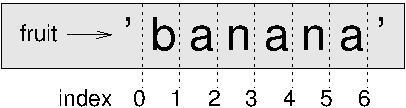
\includegraphics[scale=0.8]{figs/banana.pdf}}
\caption{Δείκτες τεμαχίων.}
\label{fig.banana}
\end{figure}


Εάν παραλείψετε τον πρώτο δείκτη (πριν την άνω κάτω τελεία), το τεμάχιο θα ξεκινήσει από την 
αρχή της συμβολοσειράς. Αν παραλείψετε τον δεύτερο δείκτη, το τεμάχιο θα φτάσει μέχρι το τέλος 
της συμβολοσειράς\en : 

\begin{verbatim}
>>> fruit = 'banana'
>>> fruit[:3]
'ban'
>>> fruit[3:]
'ana'
\end{verbatim}
%
\gr 
Αν ο πρώτος δείκτης είναι μεγαλύτερος ή ίσος με το δεύτερο το αποτέλεσμα θα είναι μία κενή 
συμβολοσειρά, η οποία αναπαριστάται από δύο μονά εισαγωγικά\en :
\index{quotation mark}

\begin{verbatim}
>>> fruit = 'banana'
>>> fruit[3:3]
''
\end{verbatim}
%
\gr 
Μία άδεια συμβολοσειρά δεν περιέχει κανένα χαρακτήρα και το μήκος της είναι 0, αλλά εκτός από 
αυτό είναι ίδια με οποιαδήποτε άλλη συμβολοσειρά.

ΑΣΚΗΣΗ 8.3.

Δοθέντος ότι η \en {\tt fruit} \gr είναι μία συμβολοσειρά, τι σημαίνει η έκφραση \en {\tt fruit[:]};\gr 
\index{copy!slice}
\index{slice!copy}



\section{Οι συμβολοσειρές είναι αμετάβλητες}
\index{mutability}
\index{immutability}
\index{string!immutable}

Ίσως μπείτε στον πειρασμό να χρησιμοποιήσετε τον τελεστή \en {\tt []} \gr στο αριστερό μέρος 
μίας εκχώρησης, με σκοπό να αλλάξετε κάποιο χαρακτήρα σε μία συμβολοσειρά. Για παράδειγμα\en :
\index{TypeError}
\index{exception!TypeError}

\begin{verbatim}
>>> greeting = 'Hello, world!'
>>> greeting[0] = 'J'
TypeError: object does not support item assignment
\end{verbatim}
%
\gr 
Το \en "\gr αντικείμενο\en " \gr στην προκειμένη περίπτωση είναι η συμβολοσειρά και το \en "\gr στοιχείο\en " \gr είναι ο χαρακτήρας 
που προσπαθήσαμε να εκχωρήσουμε. Για την ώρα, φανταστείτε ένα {\tt αντικείμενο} σαν μία τιμή, αλλά αργότερα θα βελτιώσουμε αυτόν τον 
ορισμό. Ένα {\tt στοιχείο} είναι μία από τις τιμές μέσα σε μία ακολουθία.
\index{object}
\index{item assignment}
\index{assignment!item}
\index{immutability}

Το λάθος οφείλεται στο ότι οι συμβολοσειρές είναι {\tt αμετάβλητες}, το οποίο σημαίνει ότι δεν μπορείτε να αλλάξετε μία υπάρχουσα συμβολοσειρά. Το καλύτερο που μπορείτε να κάνετε είναι να δημιουργήσετε μία νέα συμβολοσειρά η οποία θα είναι μία παραλλαγή της 
αρχικής\en :

\begin{verbatim}
>>> greeting = 'Hello, world!'
>>> new_greeting = 'J' + greeting[1:]
>>> print new_greeting
Jello, world!
\end{verbatim}
%
\gr 
Αυτό το παράδειγμα συνενώνει ένα νέο πρώτο γράμμα με ένα τεμάχιο της \en {\tt greeting}, \gr χωρίς να επηρεάζει καθόλου την αρχική 
συμβολοσειρά.
\index{concatenation}


\section{Αναζήτηση}
\label{find}

Τι κάνει η ακόλουθη συνάρτηση\en ;
\index{find function}
\index{function!find}

\begin{verbatim}
def find(word, letter):
    index = 0
    while index < len(word):
        if word[index] == letter:
            return index
        index = index + 1
    return -1
\end{verbatim}
%
\gr 
Κατά μία έννοια, η \en {\tt find} \gr είναι το αντίθετο του τελεστή \en {\tt []}. \gr
Αντί να παίρνει ένα δείκτη και να εξάγει τον αντίστοιχο χαρακτήρα, παίρνει έναν χαρακτήρα 
και βρίσκει το δείκτη στον οποίο εμφανίζεται αυτός ο χαρακτήρας. Αν ο χαρακτήρας δεν βρεθεί, 
η συνάρτηση επιστρέφει \en {\tt -1}.\gr

Αυτό είναι το πρώτο παράδειγμα που βλέπουμε με μία δήλωση \en {\tt return} \gr μέσα σε ένα βρόγχο. 
Αν η συνθήκη \en {\tt word[index] == letter} \gr γίνει αληθής τότε η συνάρτηση \en "\gr σπάει\en " \gr (βγαίνει από το βρόγχο) 
και επιστρέφει αμέσως.

Αν ο χαρακτήρας δε βρεθεί μέσα στη συμβολοσειρά, το πρόγραμμα βγαίνει ομαλά από το βρόγχο και επιστρέφει \en {\tt -1}.\gr 

Αυτό το πρότυπο υπολογισμού, διάσχιση μιας συμβολοσειράς και επιστροφή όταν βρούμε αυτό που ψάχνουμε, 
ονομάζεται αναζήτηση.
\index{traversal}
\index{search pattern}
\index{pattern!search}

ΑΣΚΗΣΗ 8.4.

Τροποποιήστε τη \en {\tt find} \gr έτσι ώστε να έχει μία τρίτη παράμετρο, 
το δείκτη από όπου πρέπει να ξεκινήσει να ψάχνει μέσα στη \en {\tt word}.\gr



\section{Επανάληψη και καταμέτρηση}
\label{counter}
\index{counter}
\index{counting and looping}
\index{looping and counting}
\index{looping!with strings}

Το ακόλουθο πρόγραμμα μετράει πόσες φορές εμφανίζεται το γράμμα \en {\tt a} \gr 
μέσα σε μία συμβολοσειρά\en :

\begin{verbatim}
word = 'banana'
count = 0
for letter in word:
    if letter == 'a':
        count = count + 1
print count
\end{verbatim}
%
\gr 
Αυτό το πρόγραμμα επιδεικνύει ένα άλλο πρότυπο υπολογισμού με όνομα \en "\gr μετρητής\en ". \gr 
Η μεταβλητή \en {\tt count} \gr αρχικοποιείται στο 0 και προσαυξάνεται κάθε φορά που βρίσκουμε ένα 
\en {\tt a}. \gr Όταν ο βρόγχος τερματίσει, η \en {\tt count} \gr περιέχει το αποτέλεσμα, το πλήθος δηλαδή 
των \en {\tt a}. \gr 

ΑΣΚΗΣΗ 8.5.
\index{encapsulation}

Ενθυλακώστε αυτόν τον κώδικα μέσα σε μία συνάρτηση με όνομα \en {\tt count}, \gr 
και γενικεύστε την ούτως ώστε να δέχεται τη συμβολοσειρά και το γράμμα σαν ορίσματα.

ΑΣΚΗΣΗ 8.6.

Ξαναγράψτε αυτή τη συνάρτηση έτσι ώστε αντί να διασχίζει τη συμβολοσειρά, να χρησιμοποιεί 
την τριών-παραμέτρων έκδοση την \en {\tt find} \gr από την προηγούμενη ενότητα.


\section{Μέθοδοι συμβολοσειρών}

Μία μέθοδος είναι παρόμοια με μία συνάρτηση, παίρνει ορίσματα και επιστρέφει μία τιμή, 
αλλά έχουν διαφορετική σύνταξη. Για παράδειγμα, η μέθοδος \en {\tt upper} \gr παίρνει μία συμβολοσειρά 
και επιστρέφει μία νέα συμβολοσειρά με όλα τα γράμματα κεφαλαία\en :
\index{method}
\index{string!method}
\gr 
Αντί για την σύνταξη συνάρτησης \en {\tt upper(word)}, \gr χρησιμοποιεί τη σύνταξη μεθόδου 
\en {\tt word.upper()}.
\index{dot notation}

\begin{verbatim}
>>> word = 'banana'
>>> new_word = word.upper()
>>> print new_word
BANANA
\end{verbatim}
%
\gr 
Αυτός ο τρόπος συμβολισμού με τελεία προσδιορίζει το όνομα της μεθόδου, \en {\tt upper}, \gr 
και το όνομα της συμβολοσειράς στην οποία θα εφαρμοστεί η μέθοδος, \en {\tt word}. \gr Οι κενές 
παρενθέσεις υποδηλώνουν ότι η μέθοδος δεν παίρνει κανένα όρισμα.
\index{parentheses!empty}

Μία κλήση μεθόδου ονομάζεται \en "\gr επίκληση\en ". \gr Σε αυτήν την περίπτωση, 
θα λέγαμε ότι επικαλούμε την \en {\tt upper} \gr στη \en {\tt word}. \gr  
\index{invocation}

Αποδεικνυεται επίσης, ότι υπάρχει και μία μέθοδος συμβολοσειρών με όνομα \en {\tt find} \gr 
η οποία εξαιρετικά παρόμοια με την συνάρτηση που γράψαμε\en :

\begin{verbatim}
>>> word = 'banana'
>>> index = word.find('a')
>>> print index
1
\end{verbatim}
%
\gr 
Σε αυτό το παράδειγμα, επικαλούμε τη \en {\tt find} \gr στη \en {\tt word} \gr 
και περνάμε το γράμμα που ψάχνουμε σαν μία παράμετρο.

Στην πραγματικότητα, η μέθοδος \en {\tt find} \gr είναι πιο γενική από την δική μας συνάρτηση 
γιατί εκτώς από χαρακτήρες μπορεί να βρει και \en "\gr υποσυμβολοσειρές\en ":

\begin{verbatim}
>>> word.find('na')
2
\end{verbatim}
%
\gr 
Μπορεί να πάρει σαν δεύτερο όρισμα το δείκτη από όπου θα πρέπει να ξεκινήσει\en :
\index{optional argument}
\index{argument!optional}

\begin{verbatim}
>>> word.find('na', 3)
4
\end{verbatim}
%
\gr 
Και σαν ένα τρίτο όρισμα, το δείκτη όπου πρέπει να σταματήσει\en :

\begin{verbatim}
>>> name = 'bob'
>>> name.find('b', 1, 2)
-1
\end{verbatim}
%
\gr 
Αυτή η αναζήτηση αναζήτηση αποτυγχάνει επειδή το \en {\tt b} \gr δεν εμφανίζεται πουθενά μέσα στο 
εύρος των δεικτών από \en {\tt 1} \gr εώς \en {\tt 2} \gr (μη συμπεριλαμβανομένου του \en {\tt 2}\gr ).


ΑΣΚΗΣΗ 8.7.
\index{count method}
\index{method!count}

Υπάρχει μία μέθοδος συμβολοσειρών με όνομα \en {\tt count} \gr η οποία είναι παρόμοια 
με τη συνάρτηση της προηγούμενης άσκησης. Διαβάστε στην τεκμηρίωση αυτής της μεθόδου και 
γράψτε μία επίκληση η οποία θα μετράει το πλήθος των \en {\tt a} \gr στην λέξη \en \verb"'banana'".\gr 


ΑΣΚΗΣΗ 8.8.
\index{string method}
\index{method!string}

Διαβάστε την τεκμηρίωση των μεθόδων συμβολοσειρών στην διεύθυνση \en 
\url{http://docs.python.org/2/library/stdtypes.html#string-methods}. \gr 
Ίσως θελήσετε να πειραματιστείτε με κάποιες από αυτές για να βεβαιωθείτε ότι 
καταλάβατε πως δουλεύουν. Η \en {\tt strip} \gr και η \en {replace} \gr είναι 
ιδιαίτερα χρήσιμες.

Η τεκμηρίωση χρησιμοποιεί μία σύνταξη η οποία να σας δυσκολεύει. Για παράδειγμα, 
στην \en \verb"find(sub[, start[, end]])", \gr οι αγκύλες υποδηλώνουν τα προαιρετικά 
ορίσματα. Άρα το \en {\tt sub} \gr είναι απαραίτητο αλλά το \en {\tt start} \gr είναι προαιρετικό, 
και αν συμπεριλάβετε το \en {\tt start} \gr τότε το \en {\tt end} \gr είναι προαιρετικό. \en


\section{$\tau\epsilon\lambda\epsilon\sigma\tau\eta\varsigma$  {\tt in}}
\label{inboth}
\index{in operator}
\index{operator!in}
\index{boolean operator}
\index{operator!boolean}
\gr 
Η λέξη \en {\tt in} \gr είναι ένας τελεστής αληθείας \en (boolean) \gr ο οποίος παίρνει 
δύο συμβολοσειρές και επιστρέφει \en {\tt True} \gr αν η πρώτη εμφανίζεται σαν μία υποσυμβολοσειρά 
μέσα στη δεύτερη\en :

\begin{verbatim}
>>> 'a' in 'banana'
True
>>> 'seed' in 'banana'
False
\end{verbatim}
%
\gr 
Για παράδειγμα, η ακόλουθη συνάρτηση εμφανίζει όλα τα γράμματα της \en 
{\tt word1} \gr τα οποία υπάρχουν και στη \en {\tt word2}:

\begin{verbatim}
def in_both(word1, word2):
    for letter in word1:
        if letter in word2:
            print letter
\end{verbatim}
%
\gr 
Με καλά επιλεγμένα ονόματα μεταβλητών, ένα πρόγραμμα σε \en Python \gr διαβάζεται μερικές φορές όπως 
ένα κείμενο στα αγγλικά. Θα μπορούσατε να διαβάσετε αυτόν το βρόχο, \en ``for (each) letter in (the first) word, 
if (the) letter (appears) in (the second) word, print (the) letter.''\gr

Παρακάτω βλέπετε τι θα παίρνατε αν συγκρίνατε μήλα \en (apples) \gr και πορτοκάλια \en (oranges):

\begin{verbatim}
>>> in_both('apples', 'oranges')
a
e
s
\end{verbatim}
%
\gr 
\section{Σύγκριση συμβολοσειρών}
\index{string!comparison}
\index{comparison!string}

Οι σχεσιακοι τελεστές δουλεύουν και με τις συμβολοσειρές. Για να δούμε αν δύο συμβολοσειρές 
είναι ίδιες\en :

\begin{verbatim}
if word == 'banana':
    print 'All right, bananas.'
\end{verbatim}
%
\gr 
Άλλοι σχεσιακοί τελεστές μας βοηθάνε να να βάζουμε λέξεις σε αλφαβητική σειρά\en :

\begin{verbatim}
if word < 'banana':
    print 'Your word,' + word + ', comes before banana.'
elif word > 'banana':
    print 'Your word,' + word + ', comes after banana.'
else:
    print 'All right, bananas.'
\end{verbatim}
%
\gr 
Η \en Python \gr δεν μπορεί να χειριστεί τα κεφαλαία και τα πεζά με τον ίδιο τρόπο 
που το κάνουμε οι άνθρωποι. Όλα τα κεφαλαία γράμματα προηγούνται όλων των πεζών γραμμάτων, 
επομένως\en :

\begin{verbatim}
Your word, Pineapple, comes before banana.
\end{verbatim}
%
\gr 
Ένας κοινός τρόπος χειρισμού αυτού του προβλήματος είναι να μετατρέπουμε τις συμβολοσειρές 
σε μία προκαθορισμένη μορφή, όπως για παράδειγμα όλα κεφαλαία, πριν εκτελέσουμε τη σύγκριση. 
Κρατήστε το αυτό κατά νου σε περίπτωση που χρειαστεί να υπερασπιστείτε τον εαυτό σας ενάντια 
σε έναν άνδρα οπλισμένο με έναν Ανανά \en(Pineapple) \gr (αμερικάνικη στρατιωτική αργκό όπου 
ο ανανάς σημαίνει χειρομβομβίδα).


\section{Αποσφαλμάτωση}
\index{debugging}
\index{traversal}

Όταν χρησιμοποιείτε δείκτες για να διασχίσετε τις τιμές σε μία ακολουθία, 
είναι περίπλοκο να πάρετε σωστά την αρχή και το τέλος της διάσχισης. Ακολουθεί 
μία συνάρτηση η οποία υποτίθεται ότι συγκρίνει δύο λέξεις και επιστρέφει \en {\tt True} \gr 
αν η μία είναι η αντίστροφη της άλλης, αλλά έχει δύο λάθη\en :

\begin{verbatim}
def is_reverse(word1, word2):
    if len(word1) != len(word2):
        return False

    i = 0
    j = len(word2)

    while j > 0:
        if word1[i] != word2[j]:
            return False
        i = i+1
        j = j-1

    return True
\end{verbatim}
%
\gr 
Η πρώτη δήλωση \en {\tt if} \gr ελέγχει εάν οι λέξεις έχουν το ίδιο μήκος. 
Αν όχι, τότε μπορούμε να επιστρέψουμε \en {\tt False} \gr αμέσως, και για το 
υπόλοιπο της συνάρτησης μπορούμε να θεωρήσουμε ότι οι λέξεις έχουν το ίδιο μήκος. 
Αυτό είναι ένα παράδειγμα πρότυπου φύλακα της Ενότητας\en ~\ref{guardian}.\gr
\index{guardian pattern}
\index{pattern!guardian}
\index{index}

Το \en {\tt i} \gr και το \en {\tt j} \gr είναι δείκτες. Ο πρώτος διασχίζει τη \en {\tt word1} \gr 
προς τα μπρος όσο ο δεύτερος διασχίζει τη \en {\tt word2} \gr προς τα πίσω. Αν βρούμε δύο γράμματα 
το οποία δεν ταιριάζουν τότε μπορούμε να επιστρέψουμε \en {\tt False} \gr αμέσως. Αν τελειώσει ολόκληρη 
η επανάληψη και όλα τα γράμματα ταιριάζουν μπορούμε να επιστρέψουμε \en {\tt True}.\gr 

Αν δοκιμάσουμε αυτήν τη συνάρτηση με τις λέξεις \en "pots" \gr και \en "stop", \gr περιμένουμε η 
επιστρεφόμενη τιμή να είναι \en {\tt True} \gr αλλά παίρνουμε ένα σφάλμα \en (IndexError):
\index{IndexError}
\index{exception!IndexError}

\begin{verbatim}
>>> is_reverse('pots', 'stop')
...
  File "reverse.py", line 15, in is_reverse
    if word1[i] != word2[j]:
IndexError: string index out of range
\end{verbatim}
%
\gr 
Η πρώτη μου κίνηση για αποσφαλμάτωση είναι να εμφανίσω τις τιμές των δεικτών ακριβώς πριν 
από τη γραμμή που εμφανίζεται το σφάλμα.\en 

\begin{verbatim}
    while j > 0:
        print i, j        # print here

        if word1[i] != word2[j]:
            return False
        i = i+1
        j = j-1
\end{verbatim}
%
\gr 
Αν ξανατρέξω τώρα το πρόγραμμα θα πάρω περισσότερες πληροφορίες\en :

\begin{verbatim}
>>> is_reverse('pots', 'stop')
0 4
...
IndexError: string index out of range
\end{verbatim}
%
\gr 
Στην πρώτη επανάληψη του βρόγχου, η τιμή του \en {\tt j} \gr είναι 4, η οποία είναι εκτός εύρους 
για τη συμβολοσειρά \en \verb"'pots'". \gr Ο δείκτης για τον τελευταίο χαρακτήρα είναι 3, άρα η αρχική 
τιμή για το \en {\tt j} \gr θα πρέπει να είναι \en {\tt len(word2)-1}.
\index{semantic error}
\index{error!semantic}
\gr 

Αν φτιάξω αυτό το σφάλμα και τρέξω ξανά το πρόγραμμα παίρνω\en :

\begin{verbatim}
>>> is_reverse('pots', 'stop')
0 3
1 2
2 1
True
\end{verbatim}
%
\gr 
Αυτή τη φορά παίρνουμε τη σωστή απάντηση, αλλά φαίνεται σαν να εκτελείτε μόνο τρεις φορές η επανάληψη, το 
οποίο είναι ύποπτο. Για να έχουμε μια καλύτερη ιδέα του τι συμβαίνει, είναι χρήσιμο να σχεδιάσουμε ένα 
διάγραμμα κατάστασης. Κατά τη διάρκεια της πρώτης επανάληψης, το πλαίσιο για την \en \verb"is_reverse" \gr 
εμφανίζεται στο σχημα\en ~\ref{fig.state4}. \gr 
\index{state diagram}
\index{diagram!state}

\begin{figure}
\centerline
{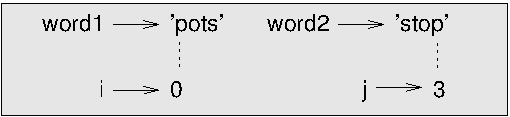
\includegraphics[scale=0.8]{figs/state4.pdf}}
\caption{Διάγραμμα κατάστασης.}
\label{fig.state4}
\end{figure}

Τοποθέτησα τις μεταβλητές μέσα στο πλαίσιο και πρόσθεσα διακεκομμένες λίγο αυθαίρετα για να δείξω 
ότι οι τιμές του \en {\tt i} \gr και του \en {\tt j} \gr δείχνουν χαρατκήρες στην \en {\tt word1} \gr 
και στην \en {\tt word2}.\gr 

ΑΣΚΗΣΗ 8.9.
\label{isreverse}

Ξεκινώντας με αυτό το διάγραμμα, εκτελέστε το πρόγραμμα στο χαρτί, αλλάζοντας 
τις τιμές των \en {\tt i} \gr και \en {\tt j} \gr σε κάθε επανάληψη. Βρείτε και 
διορθώστε το δεύτερο λάθος σε αυτήν τη συνάρτηση.




\section{Glossary}

\begin{description}

\item[object:] Something a variable can refer to.  For now,
you can use ``object'' and ``value'' interchangeably.
\index{object}

\item[sequence:] An ordered set; that is, a set of
values where each value is identified by an integer index.
\index{sequence}

\item[item:] One of the values in a sequence.
\index{item}

\item[index:] An integer value used to select an item in
a sequence, such as a character in a string.
\index{index}

\item[slice:] A part of a string specified by a range of indices.
\index{slice}

\item[empty string:] A string with no characters and length 0, represented
by two quotation marks.
\index{empty string}

\item[immutable:] The property of a sequence whose items cannot
be assigned.
\index{immutability}

\item[traverse:] To iterate through the items in a sequence,
performing a similar operation on each.
\index{traversal}

\item[search:] A pattern of traversal that stops
when it finds what it is looking for.
\index{search pattern}
\index{pattern!search}

\item[counter:] A variable used to count something, usually initialized
to zero and then incremented.
\index{counter}

\item[method:] A function that is associated with an object and called
using dot notation.
\index{method}

\item[invocation:] A statement that calls a method.
\index{invocation}

\end{description}


\section{Exercises}

\begin{exercise}
\index{step size}
\index{slice operator}
\index{operator!slice}

A string slice can take a third index that specifies the ``step
size;'' that is, the number of spaces between successive characters.
A step size of 2 means every other character; 3 means every third,
etc.

\begin{verbatim}
>>> fruit = 'banana'
>>> fruit[0:5:2]
'bnn'
\end{verbatim}

A step size of -1 goes through the word backwards, so
the slice \verb"[::-1]" generates a reversed string.
\index{palindrome}

Use this idiom to write a one-line version of \verb"is_palindrome"
from Exercise~\ref{palindrome}.
\end{exercise}


\begin{exercise}

The following functions are all {\em intended} to check whether a
string contains any lowercase letters, but at least some of them are
wrong.  For each function, describe what the function actually does
(assuming that the parameter is a string).

\begin{verbatim}
def any_lowercase1(s):
    for c in s:
        if c.islower():
            return True
        else:
            return False

def any_lowercase2(s):
    for c in s:
        if 'c'.islower():
            return 'True'
        else:
            return 'False'

def any_lowercase3(s):
    for c in s:
        flag = c.islower()
    return flag

def any_lowercase4(s):
    flag = False
    for c in s:
        flag = flag or c.islower()
    return flag

def any_lowercase5(s):
    for c in s:
        if not c.islower():
            return False
    return True
\end{verbatim}

\end{exercise}


\begin{exercise}
\index{letter rotation}
\index{rotation, letter}

\label{exrotate}
ROT13 is a weak form of encryption that involves ``rotating'' each
letter in a word by 13 places.  To rotate a letter means
to shift it through the alphabet, wrapping around to the beginning if
necessary, so 'A' shifted by 3 is 'D' and 'Z' shifted by 1 is 'A'.

Write a function called \verb"rotate_word"
that takes a string and an integer as parameters, and that returns
a new string that contains the letters from the original string
``rotated'' by the given amount.

For example, ``cheer'' rotated by 7 is ``jolly'' and ``melon'' rotated
by -10 is ``cubed''.

%For example ``sleep''
%rotated by 9 is ``bunny'' and ``latex'' rotated by 7 is ``shale''.

You might want to use the built-in functions {\tt ord}, which converts
a character to a numeric code, and {\tt chr}, which converts numeric
codes to characters.

Potentially offensive jokes on the Internet are sometimes encoded
in ROT13.  If you are not easily offended, find and decode some
of them.  Solution: \url{http://thinkpython.com/code/rotate.py}.

\end{exercise}


\chapter{Case study: word play}

\section{Reading word lists}
\label{wordlist}

For the exercises in this chapter we need a list of English words.
There are lots of word lists available on the Web, but the one most
suitable for our purpose is one of the word lists collected and
contributed to the public domain by Grady Ward as part of the Moby
lexicon project (see \url{http://wikipedia.org/wiki/Moby_Project}).  It
is a list of 113,809 official crosswords; that is, words that are
considered valid in crossword puzzles and other word games.  In the
Moby collection, the filename is {\tt 113809of.fic}; you can download
a copy, with the simpler name {\tt words.txt}, from
\url{http://thinkpython.com/code/words.txt}.
\index{Moby Project}
\index{crosswords}

This file is in plain text, so you can open it with a text
editor, but you can also read it from Python.  The built-in
function {\tt open} takes the name of the file as a parameter
and returns a {\bf file object} you can use to read the file.
\index{open function}
\index{function!open}
\index{plain text}
\index{text!plain}
\index{object!file}
\index{file object}

\begin{verbatim}
>>> fin = open('words.txt')
>>> print fin
<open file 'words.txt', mode 'r' at 0xb7f4b380>
\end{verbatim}
%
{\tt fin} is a common name for a file object used for
input.  Mode \verb"'r'" indicates that this file is open for
reading (as opposed to \verb"'w'" for writing).
\index{readline method}
\index{method!readline}

The file object provides several methods for reading, including
{\tt readline}, which reads characters from the file
until it gets to a newline and returns the result as a
string:

\begin{verbatim}
>>> fin.readline()
'aa\r\n'
\end{verbatim}
%
The first word in this particular list is ``aa,'' which is a kind of
lava.  The sequence \verb"\r\n" represents two whitespace characters,
a carriage return and a newline, that separate this word from the
next.

The file object keeps track of where it is in the file, so
if you call {\tt readline} again, you get the next word:

\begin{verbatim}
>>> fin.readline()
'aah\r\n'
\end{verbatim}
%
The next word is ``aah,'' which is a perfectly legitimate
word, so stop looking at me like that.
Or, if it's the whitespace that's bothering you,
we can get rid of it with the string method {\tt strip}:
\index{strip method}
\index{method!strip}

\begin{verbatim}
>>> line = fin.readline()
>>> word = line.strip()
>>> print word
aahed
\end{verbatim}
%
You can also use a file object as part of a {\tt for} loop.
This program reads {\tt words.txt} and prints each word, one
per line:
\index{open function}
\index{function!open}

\begin{verbatim}
fin = open('words.txt')
for line in fin:
    word = line.strip()
    print word
\end{verbatim}
%

\begin{exercise}

Write a program that reads {\tt words.txt} and prints only the
words with more than 20 characters (not counting whitespace).
\index{whitespace}

\end{exercise}


\section{Exercises}

There are solutions to these exercises in the next section.
You should at least attempt each one before you read the solutions.

\begin{exercise}

In 1939 Ernest Vincent Wright published a 50,000 word novel called
{\em Gadsby} that does not contain the letter ``e.''  Since ``e'' is
the most common letter in English, that's not easy to do.

In fact, it is difficult to construct a solitary thought without using
that most common symbol.  It is slow going at first, but with caution
and hours of training you can gradually gain facility.

All right, I'll stop now.

Write a function called \verb"has_no_e" that returns {\tt True} if
the given word doesn't have the letter ``e'' in it.

Modify your program from the previous section to print only the words
that have no ``e'' and compute the percentage of the words in the list
have no ``e.''
\index{lipogram}

\end{exercise}


\begin{exercise}

Write a function named {\tt avoids}
that takes a word and a string of forbidden letters, and
that returns {\tt True} if the word doesn't use any of the forbidden
letters.

Modify your program to prompt the user to enter a string
of forbidden letters and then print the number of words that
don't contain any of them.
Can you find a combination of 5 forbidden letters that
excludes the smallest number of words?

\end{exercise}



\begin{exercise}

Write a function named \verb"uses_only" that takes a word and a
string of letters, and that returns {\tt True} if the word contains
only letters in the list.  Can you make a sentence using only the
letters {\tt acefhlo}?  Other than ``Hoe alfalfa?''

\end{exercise}


\begin{exercise}

Write a function named \verb"uses_all" that takes a word and a
string of required letters, and that returns {\tt True} if the word
uses all the required letters at least once.  How many words are there
that use all the vowels {\tt aeiou}?  How about {\tt aeiouy}?

\end{exercise}


\begin{exercise}

Write a function called \verb"is_abecedarian" that returns
{\tt True} if the letters in a word appear in alphabetical order
(double letters are ok).
How many abecedarian words are there?

\index{abecedarian}

\end{exercise}


%\begin{exercise}
%\label{palindrome}
%A palindrome is a word that reads the same
%forward and backward, like ``rotator'' and ``noon.''
%Write a boolean function named \verb"is_palindrome" that
%takes a string as a parameter and returns {\tt True} if it is
%a palindrome.

%Modify your program from the previous section to print all
%of the palindromes in the word list and then print the total
%number of palindromes.
%\end{exercise}



\section{Search}
\index{search pattern}
\index{pattern!search}

All of the exercises in the previous section have something
in common; they can be solved with the search pattern we saw
in Section~\ref{find}.  The simplest example is:

\begin{verbatim}
def has_no_e(word):
    for letter in word:
        if letter == 'e':
            return False
    return True
\end{verbatim}
%
The {\tt for} loop traverses the characters in {\tt word}.  If we find
the letter ``e'', we can immediately return {\tt False}; otherwise we
have to go to the next letter.  If we exit the loop normally, that
means we didn't find an ``e'', so we return {\tt True}.
\index{traversal}

% Removing this because we haven't seen the in operator yet.
%\index{in operator}
%\index{operator!in}

%You could write this function more concisely using the {\tt in}
%operator, but I started with this version because it
%demonstrates the logic of the search pattern.
\index{generalization}

{\tt avoids} is a more general version of \verb"has_no_e" but it
has the same structure:

\begin{verbatim}
def avoids(word, forbidden):
    for letter in word:
        if letter in forbidden:
            return False
    return True
\end{verbatim}
%
We can return {\tt False} as soon as we find a forbidden letter;
if we get to the end of the loop, we return {\tt True}.

\verb"uses_only" is similar except that the sense of the condition
is reversed:

\begin{verbatim}
def uses_only(word, available):
    for letter in word:
        if letter not in available:
            return False
    return True
\end{verbatim}
%
Instead of a list of forbidden letters, we have a list of available
letters.  If we find a letter in {\tt word} that is not in
{\tt available}, we can return {\tt False}.

\verb"uses_all" is similar except that we reverse the role
of the word and the string of letters:

\begin{verbatim}
def uses_all(word, required):
    for letter in required:
        if letter not in word:
            return False
    return True
\end{verbatim}
%
Instead of traversing the letters in {\tt word}, the loop
traverses the required letters.  If any of the required letters
do not appear in the word, we can return {\tt False}.
\index{traversal}

If you were really thinking like a computer scientist, you would
have recognized that \verb"uses_all" was an instance of a
previously-solved problem, and you would have written:

\begin{verbatim}
def uses_all(word, required):
    return uses_only(required, word)
\end{verbatim}
%
This is an example of a program development method called {\bf problem
recognition}, which means that you recognize the problem you are
working on as an instance of a previously-solved problem, and apply a
previously-developed solution.
\index{problem recognition}
\index{development plan!problem recognition}


\section{Looping with indices}
\index{looping!with indices}
\index{index!looping with}

I wrote the functions in the previous section with {\tt for}
loops because I only needed the characters in the strings; I didn't
have to do anything with the indices.

For \verb"is_abecedarian" we have to compare adjacent letters,
which is a little tricky with a {\tt for} loop:

\begin{verbatim}
def is_abecedarian(word):
    previous = word[0]
    for c in word:
        if c < previous:
            return False
        previous = c
    return True
\end{verbatim}


An alternative is to
use recursion:

\begin{verbatim}
def is_abecedarian(word):
    if len(word) <= 1:
        return True
    if word[0] > word[1]:
        return False
    return is_abecedarian(word[1:])
\end{verbatim}

Another option is to use a {\tt while} loop:

\begin{verbatim}
def is_abecedarian(word):
    i = 0
    while i < len(word)-1:
        if word[i+1] < word[i]:
            return False
        i = i+1
    return True
\end{verbatim}
%
The loop starts at {\tt i=0} and ends when {\tt i=len(word)-1}.  Each
time through the loop, it compares the $i$th character (which you can
think of as the current character) to the $i+1$th character (which you
can think of as the next).

If the next character is less than (alphabetically before) the current
one, then we have discovered a break in the abecedarian trend, and
we return {\tt False}.

If we get to the end of the loop without finding a fault, then the
word passes the test.  To convince yourself that the loop ends
correctly, consider an example like \verb"'flossy'".  The
length of the word is 6, so
the last time the loop runs is when {\tt i} is 4, which is the
index of the second-to-last character.  On the last iteration,
it compares the second-to-last character to the last, which is
what we want.
\index{palindrome}

Here is a version of \verb"is_palindrome" (see
Exercise~\ref{palindrome}) that uses two indices; one starts at the
beginning and goes up; the other starts at the end and goes down.

\begin{verbatim}
def is_palindrome(word):
    i = 0
    j = len(word)-1

    while i<j:
        if word[i] != word[j]:
            return False
        i = i+1
        j = j-1

    return True
\end{verbatim}

Or, if you noticed that this is an instance of a previously-solved
problem, you might have written:

\begin{verbatim}
def is_palindrome(word):
    return is_reverse(word, word)
\end{verbatim}
\index{problem recognition}
\index{development plan!problem recognition}

Assuming you did Exercise~\ref{isreverse}.


\section{Debugging}
\index{debugging}
\index{testing!is hard}
\index{program testing}

Testing programs is hard.  The functions in this chapter are
relatively easy to test because you can check the results by hand.
Even so, it is somewhere between difficult and impossible to choose a
set of words that test for all possible errors.

Taking \verb"has_no_e" as an example, there are two obvious
cases to check: words that have an 'e' should return {\tt False};
words that don't should return {\tt True}.  You should have no
trouble coming up with one of each.

Within each case, there are some less obvious subcases.  Among the
words that have an ``e,'' you should test words with an ``e'' at the
beginning, the end, and somewhere in the middle.  You should test long
words, short words, and very short words, like the empty string.  The
empty string is an example of a {\bf special case}, which is one of
the non-obvious cases where errors often lurk.
\index{special case}

In addition to the test cases you generate, you can also test
your program with a word list like {\tt words.txt}.  By scanning
the output, you might be able to catch errors, but be careful:
you might catch one kind of error (words that should not be
included, but are) and not another (words that should be included,
but aren't).

In general, testing can help you find bugs, but it is not easy to
generate a good set of test cases, and even if you do, you can't
be sure your program is correct.
\index{testing!and absence of bugs}

According to a legendary computer scientist:

\begin{quote}
Program testing can be used to show the presence of bugs, but never to
show their absence!

--- Edsger W. Dijkstra
\end{quote}
\index{Dijkstra, Edsger}


\section{Glossary}

\begin{description}

\item[file object:] A value that represents an open file.
\index{file object}
\index{object!file}

\item[problem recognition:] A way of solving a problem by
expressing it as an instance of a previously-solved problem.
\index{problem recognition}

\item[special case:] A test case that is atypical or non-obvious
(and less likely to be handled correctly).
\index{special case}

\end{description}


\section{Exercises}

\begin{exercise}
\index{Car Talk}
\index{Puzzler}
\index{double letters}

This question is based on a Puzzler that was broadcast on the radio
program {\em Car Talk}
(\url{http://www.cartalk.com/content/puzzlers}):

\begin{quote}
Give me a word with three consecutive double letters. I'll give you a
couple of words that almost qualify, but don't. For example, the word
committee, c-o-m-m-i-t-t-e-e. It would be great except for the `i' that
sneaks in there. Or Mississippi: M-i-s-s-i-s-s-i-p-p-i. If you could
take out those i's it would work. But there is a word that has three
consecutive pairs of letters and to the best of my knowledge this may
be the only word. Of course there are probably 500 more but I can only
think of one. What is the word?
\end{quote}

Write a program to find it.  Solution: \url{http://thinkpython.com/code/cartalk1.py}.

\end{exercise}


\begin{exercise}
Here's another {\em Car Talk}
Puzzler (\url{http://www.cartalk.com/content/puzzlers}):
\index{Car Talk}
\index{Puzzler}
\index{odometer}
\index{palindrome}

\begin{quote}
``I was driving on the highway the other day and I happened to
notice my odometer. Like most odometers, it shows six digits,
in whole miles only. So, if my car had 300,000
miles, for example, I'd see 3-0-0-0-0-0.

``Now, what I saw that day was very interesting. I noticed that the
last 4 digits were palindromic; that is, they read the same forward as
backward. For example, 5-4-4-5 is a palindrome, so my odometer
could have read 3-1-5-4-4-5.

``One mile later, the last 5 numbers were palindromic. For example, it
could have read 3-6-5-4-5-6.  One mile after that, the middle 4 out of
6 numbers were palindromic.  And you ready for this? One mile later,
all 6 were palindromic!

``The question is, what was on the odometer when I first looked?''
\end{quote}

Write a Python program that tests all the six-digit numbers and prints
any numbers that satisfy these requirements.
Solution: \url{http://thinkpython.com/code/cartalk2.py}.

\end{exercise}


\begin{exercise}
Here's another {\em Car Talk} Puzzler you can solve with a
search (\url{http://www.cartalk.com/content/puzzlers}):
\index{Car Talk}
\index{Puzzler}
\index{palindrome}

\begin{quote}
``Recently I had a visit with my mom and we realized that
the two digits that make up my age when reversed resulted in her
age. For example, if she's 73, I'm 37. We wondered how often this has
happened over the years but we got sidetracked with other topics and
we never came up with an answer.

``When I got home I figured out that the digits of our ages have been
reversible six times so far. I also figured out that if we're lucky it
would happen again in a few years, and if we're really lucky it would
happen one more time after that. In other words, it would have
happened 8 times over all. So the question is, how old am I now?''

\end{quote}

Write a Python program that searches for solutions to this Puzzler.
Hint: you might find the string method {\tt zfill} useful.

Solution: \url{http://thinkpython.com/code/cartalk3.py}.

\end{exercise}



\chapter{Lists}

\section{A list is a sequence}
\label{sequence}

Like a string, a {\bf list} is a sequence of values.  In a string, the
values are characters; in a list, they can be any type.  The values in
a list are called {\bf elements} or sometimes {\bf items}.
\index{list}
\index{type!list}
\index{element}
\index{sequence}
\index{item}

There are several ways to create a new list; the simplest is to
enclose the elements in square brackets (\verb"[" and \verb"]"):

\begin{verbatim}
[10, 20, 30, 40]
['crunchy frog', 'ram bladder', 'lark vomit']
\end{verbatim}
%
The first example is a list of four integers.  The second is a list of
three strings.  The elements of a list don't have to be the same type.
The following list contains a string, a float, an integer, and
(lo!) another list:

\begin{verbatim}
['spam', 2.0, 5, [10, 20]]
\end{verbatim}
%
A list within another list is {\bf nested}.
\index{nested list}
\index{list!nested}

A list that contains no elements is
called an empty list; you can create one with empty
brackets, \verb"[]".
\index{empty list}
\index{list!empty}

As you might expect, you can assign list values to variables:

\begin{verbatim}
>>> cheeses = ['Cheddar', 'Edam', 'Gouda']
>>> numbers = [17, 123]
>>> empty = []
>>> print cheeses, numbers, empty
['Cheddar', 'Edam', 'Gouda'] [17, 123] []
\end{verbatim}
%
\index{assignment}


\section{Lists are mutable}
\label{mutable}
\index{list!element}
\index{access}
\index{index}
\index{bracket operator}
\index{operator!bracket}

The syntax for accessing the elements of a list is the same as for
accessing the characters of a string---the bracket operator.  The
expression inside the brackets specifies the index.  Remember that the
indices start at 0:

\begin{verbatim}
>>> print cheeses[0]
Cheddar
\end{verbatim}
%
Unlike strings, lists are mutable.  When the bracket operator appears
on the left side of an assignment, it identifies the element of the
list that will be assigned.
\index{mutability}

\begin{verbatim}
>>> numbers = [17, 123]
>>> numbers[1] = 5
>>> print numbers
[17, 5]
\end{verbatim}
%
The one-eth element of {\tt numbers}, which
used to be 123, is now 5.
\index{index!starting at zero}
\index{zero, index starting at}

You can think of a list as a relationship between indices and
elements.  This relationship is called a {\bf mapping}; each index
``maps to'' one of the elements.  Figure~\ref{fig.liststate} shows
the state diagram for {\tt
cheeses}, {\tt numbers} and {\tt empty}:
\index{state diagram}
\index{diagram!state}
\index{mapping}

\begin{figure}
\centerline
{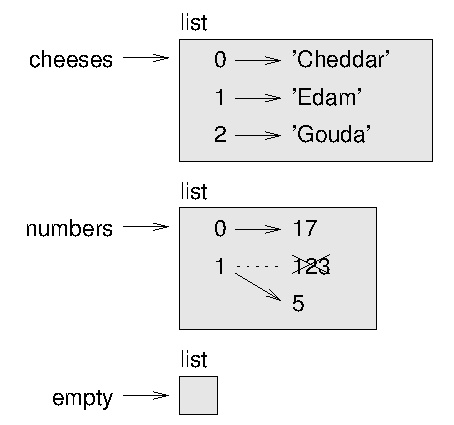
\includegraphics[scale=0.8]{figs/liststate.pdf}}
\caption{State diagram.}
\label{fig.liststate}
\end{figure}

Lists are represented by boxes with the word ``list'' outside
and the elements of the list inside.  {\tt cheeses} refers to
a list with three elements indexed 0, 1 and 2.
{\tt numbers} contains two elements; the diagram shows that the
value of the second element has been reassigned from 123 to 5.
{\tt empty} refers to a list with no elements.
\index{item assignment}
\index{assignment!item}

List indices work the same way as string indices:

\begin{itemize}

\item Any integer expression can be used as an index.

\item If you try to read or write an element that does not exist, you
get an {\tt IndexError}.
\index{exception!IndexError}
\index{IndexError}

\item If an index has a negative value, it counts backward from the
end of the list.

\end{itemize}
\index{list!index}

\index{list!membership}
\index{membership!list}
\index{in operator}
\index{operator!in}

The {\tt in} operator also works on lists.

\begin{verbatim}
>>> cheeses = ['Cheddar', 'Edam', 'Gouda']
>>> 'Edam' in cheeses
True
>>> 'Brie' in cheeses
False
\end{verbatim}


\section{Traversing a list}
\index{list!traversal}
\index{traversal!list}
\index{for loop}
\index{loop!for}
\index{statement!for}

The most common way to traverse the elements of a list is
with a {\tt for} loop.  The syntax is the same as for strings:

\begin{verbatim}
for cheese in cheeses:
    print cheese
\end{verbatim}
%
This works well if you only need to read the elements of the
list.  But if you want to write or update the elements, you
need the indices.  A common way to do that is to combine
the functions {\tt range} and {\tt len}:
\index{looping!with indices}
\index{index!looping with}

\begin{verbatim}
for i in range(len(numbers)):
    numbers[i] = numbers[i] * 2
\end{verbatim}
%
This loop traverses the list and updates each element.  {\tt len}
returns the number of elements in the list.  {\tt range} returns
a list of indices from 0 to $n-1$, where $n$ is the length of
the list.  Each time through the loop {\tt i} gets the index
of the next element.  The assignment statement in the body uses
{\tt i} to read the old value of the element and to assign the
new value.
\index{item update}
\index{update!item}

A {\tt for} loop over an empty list never executes the body:

\begin{verbatim}
for x in []:
    print 'This never happens.'
\end{verbatim}
%
Although a list can contain another list, the nested
list still counts as a single element.  The length of this list is
four:
\index{nested list}
\index{list!nested}

\begin{verbatim}
['spam', 1, ['Brie', 'Roquefort', 'Pol le Veq'], [1, 2, 3]]
\end{verbatim}



\section{List operations}
\index{list!operation}

The {\tt +} operator concatenates lists:
\index{concatenation!list}
\index{list!concatenation}

\begin{verbatim}
>>> a = [1, 2, 3]
>>> b = [4, 5, 6]
>>> c = a + b
>>> print c
[1, 2, 3, 4, 5, 6]
\end{verbatim}
%
Similarly, the {\tt *} operator repeats a list a given number of times:
\index{repetition!list}
\index{list!repetition}

\begin{verbatim}
>>> [0] * 4
[0, 0, 0, 0]
>>> [1, 2, 3] * 3
[1, 2, 3, 1, 2, 3, 1, 2, 3]
\end{verbatim}
%
The first example repeats {\tt [0]} four times.  The second example
repeats the list {\tt [1, 2, 3]} three times.


\section{List slices}
\index{slice operator}
\index{operator!slice}
\index{index!slice}
\index{list!slice}
\index{slice!list}

The slice operator also works on lists:

\begin{verbatim}
>>> t = ['a', 'b', 'c', 'd', 'e', 'f']
>>> t[1:3]
['b', 'c']
>>> t[:4]
['a', 'b', 'c', 'd']
>>> t[3:]
['d', 'e', 'f']
\end{verbatim}
%
If you omit the first index, the slice starts at the beginning.
If you omit the second, the slice goes to the end.  So if you
omit both, the slice is a copy of the whole list.
\index{list!copy}
\index{slice!copy}
\index{copy!slice}

\begin{verbatim}
>>> t[:]
['a', 'b', 'c', 'd', 'e', 'f']
\end{verbatim}
%
Since lists are mutable, it is often useful to make a copy
before performing operations that fold, spindle or mutilate
lists.
\index{mutability}

A slice operator on the left side of an assignment
can update multiple elements:
\index{slice!update}
\index{update!slice}

\begin{verbatim}
>>> t = ['a', 'b', 'c', 'd', 'e', 'f']
>>> t[1:3] = ['x', 'y']
>>> print t
['a', 'x', 'y', 'd', 'e', 'f']
\end{verbatim}
%

% You can add elements to a list by squeezing them into an empty
% slice:

% % \begin{verbatim}
% >>> t = ['a', 'd', 'e', 'f']
% >>> t[1:1] = ['b', 'c']
% >>> print t
% ['a', 'b', 'c', 'd', 'e', 'f']
% \end{verbatim}
% \afterverb
%
% And you can remove elements from a list by assigning the empty list to
% them:

% % \begin{verbatim}
% >>> t = ['a', 'b', 'c', 'd', 'e', 'f']
% >>> t[1:3] = []
% >>> print t
% ['a', 'd', 'e', 'f']
% \end{verbatim}
% \afterverb
%
% But both of those operations can be expressed more clearly
% with list methods.


\section{List methods}
\index{list!method}
\index{method, list}

Python provides methods that operate on lists.  For example,
{\tt append} adds a new element to the end of a list:
\index{append method}
\index{method!append}

\begin{verbatim}
>>> t = ['a', 'b', 'c']
>>> t.append('d')
>>> print t
['a', 'b', 'c', 'd']
\end{verbatim}
%
{\tt extend} takes a list as an argument and appends all of
the elements:
\index{extend method}
\index{method!extend}

\begin{verbatim}
>>> t1 = ['a', 'b', 'c']
>>> t2 = ['d', 'e']
>>> t1.extend(t2)
>>> print t1
['a', 'b', 'c', 'd', 'e']
\end{verbatim}
%
This example leaves {\tt t2} unmodified.

{\tt sort} arranges the elements of the list from low to high:
\index{sort method}
\index{method!sort}

\begin{verbatim}
>>> t = ['d', 'c', 'e', 'b', 'a']
>>> t.sort()
>>> print t
['a', 'b', 'c', 'd', 'e']
\end{verbatim}
%
List methods are all void; they modify the list and return {\tt None}.
If you accidentally write {\tt t = t.sort()}, you will be disappointed
with the result.
\index{void method}
\index{method!void}
\index{None special value}
\index{special value!None}


\section{Map, filter and reduce}

To add up all the numbers in a list, you can use a loop like this:

% see add.py

\begin{verbatim}
def add_all(t):
    total = 0
    for x in t:
        total += x
    return total
\end{verbatim}
%
{\tt total} is initialized to 0.  Each time through the loop,
{\tt x} gets one element from the list.  The {\tt +=} operator
provides a short way to update a variable.  This
{\bf augmented assignment statement}:
\index{update operator}
\index{operator!update}
\index{assignment!augmented}
\index{augmented assignment}

\begin{verbatim}
    total += x
\end{verbatim}
%
is equivalent to:

\begin{verbatim}
    total = total + x
\end{verbatim}
%
As the loop executes, {\tt total} accumulates the sum of the
elements; a variable used this way is sometimes called an
{\bf accumulator}.
\index{accumulator!sum}

Adding up the elements of a list is such a common operation
that Python provides it as a built-in function, {\tt sum}:

\begin{verbatim}
>>> t = [1, 2, 3]
>>> sum(t)
6
\end{verbatim}
%
An operation like this that combines a sequence of elements into
a single value is sometimes called {\bf reduce}.
\index{reduce pattern}
\index{pattern!reduce}
\index{traversal}

\begin{exercise}

Write a function called \verb"nested_sum" that takes a nested list
of integers and add up the elements from all of the nested lists.

\end{exercise}

Sometimes you want to traverse one list while building
another.  For example, the following function takes a list of strings
and returns a new list that contains capitalized strings:

\begin{verbatim}
def capitalize_all(t):
    res = []
    for s in t:
        res.append(s.capitalize())
    return res
\end{verbatim}
%
{\tt res} is initialized with an empty list; each time through
the loop, we append the next element.  So {\tt res} is another
kind of accumulator.
\index{accumulator!list}

An operation like \verb"capitalize_all" is sometimes called a {\bf
map} because it ``maps'' a function (in this case the method {\tt
capitalize}) onto each of the elements in a sequence.
\index{map pattern}
\index{pattern!map}
\index{filter pattern}
\index{pattern!filter}

\begin{exercise}

Use \verb"capitalize_all" to write a function named \verb"capitalize_nested"
that takes a nested list of strings and returns a new nested list
with all strings capitalized.

\end{exercise}

Another common operation is to select some of the elements from
a list and return a sublist.  For example, the following
function takes a list of strings and returns a list that contains
only the uppercase strings:

\begin{verbatim}
def only_upper(t):
    res = []
    for s in t:
        if s.isupper():
            res.append(s)
    return res
\end{verbatim}
%
{\tt isupper} is a string method that returns {\tt True} if
the string contains only upper case letters.

An operation like \verb"only_upper" is called a {\bf filter} because
it selects some of the elements and filters out the others.

Most common list operations can be expressed as a combination
of map, filter and reduce.  Because these operations are
so common, Python provides language features to support them,
including the built-in function {\tt map} and an operator
called a ``list comprehension.''
\index{list!comprehension}

\begin{exercise}
\label{cumulative}
\index{cumulative sum}

Write a function that takes a list of numbers and returns the
cumulative sum; that is, a new list where the $i$th element
is the sum of the first $i+1$ elements from the original list.
For example, the cumulative sum of {\tt [1, 2, 3]} is
{\tt [1, 3, 6]}.
\end{exercise}


\section{Deleting elements}
\index{element deletion}
\index{deletion, element of list}

There are several ways to delete elements from a list.  If you
know the index of the element you want, you can use
{\tt pop}:
\index{pop method}
\index{method!pop}

\begin{verbatim}
>>> t = ['a', 'b', 'c']
>>> x = t.pop(1)
>>> print t
['a', 'c']
>>> print x
b
\end{verbatim}
%
{\tt pop} modifies the list and returns the element that was removed.
If you don't provide an index, it deletes and returns the
last element.

If you don't need the removed value, you can use the {\tt del}
operator:
\index{del operator}
\index{operator!del}

\begin{verbatim}
>>> t = ['a', 'b', 'c']
>>> del t[1]
>>> print t
['a', 'c']
\end{verbatim}
%

If you know the element you want to remove (but not the index), you
can use {\tt remove}:
\index{remove method}
\index{method!remove}

\begin{verbatim}
>>> t = ['a', 'b', 'c']
>>> t.remove('b')
>>> print t
['a', 'c']
\end{verbatim}
%
The return value from {\tt remove} is {\tt None}.
\index{None special value}
\index{special value!None}

To remove more than one element, you can use {\tt del} with
a slice index:

\begin{verbatim}
>>> t = ['a', 'b', 'c', 'd', 'e', 'f']
>>> del t[1:5]
>>> print t
['a', 'f']
\end{verbatim}
%
As usual, the slice selects all the elements up to, but not
including, the second index.

\begin{exercise}

Write a function called \verb"middle" that takes a list and
returns a new list that contains all but the first and last
elements.  So \verb"middle([1,2,3,4])" should return \verb"[2,3]".

\end{exercise}

\begin{exercise}

Write a function called \verb"chop" that takes a list, modifies it
by removing the first and last elements, and returns {\tt None}.

\end{exercise}


\section{Lists and strings}
\index{list}
\index{string}
\index{sequence}

A string is a sequence of characters and a list is a sequence
of values, but a list of characters is not the same as a
string.  To convert from a string to a list of characters,
you can use {\tt list}:
\index{list!function}
\index{function!list}

\begin{verbatim}
>>> s = 'spam'
>>> t = list(s)
>>> print t
['s', 'p', 'a', 'm']
\end{verbatim}
%
Because {\tt list} is the name of a built-in function, you should
avoid using it as a variable name.  I also avoid {\tt l} because
it looks too much like {\tt 1}.  So that's why I use {\tt t}.

The {\tt list} function breaks a string into individual letters.  If
you want to break a string into words, you can use the {\tt split}
method:
\index{split method}
\index{method!split}

\begin{verbatim}
>>> s = 'pining for the fjords'
>>> t = s.split()
>>> print t
['pining', 'for', 'the', 'fjords']
\end{verbatim}
%
An optional argument called a {\bf delimiter} specifies which
characters to use as word boundaries.
The following example
uses a hyphen as a delimiter:
\index{optional argument}
\index{argument!optional}
\index{delimiter}

\begin{verbatim}
>>> s = 'spam-spam-spam'
>>> delimiter = '-'
>>> s.split(delimiter)
['spam', 'spam', 'spam']
\end{verbatim}
%
{\tt join} is the inverse of {\tt split}.  It
takes a list of strings and
concatenates the elements.  {\tt join} is a string method,
so you have to invoke it on the delimiter and pass the
list as a parameter:
\index{join method}
\index{method!join}
\index{concatenation}

\begin{verbatim}
>>> t = ['pining', 'for', 'the', 'fjords']
>>> delimiter = ' '
>>> delimiter.join(t)
'pining for the fjords'
\end{verbatim}
%
In this case the delimiter is a space character, so
{\tt join} puts a space between words.  To concatenate
strings without spaces, you can use the empty string,
\verb"''", as a delimiter.
\index{empty string}
\index{string!empty}


\section{Objects and values}
\index{object}
\index{value}

If we execute these assignment statements:

\begin{verbatim}
a = 'banana'
b = 'banana'
\end{verbatim}
%
We know that {\tt a} and {\tt b} both refer to a
string, but we don't
know whether they refer to the {\em same} string.
There are two possible states, shown in Figure~\ref{fig.list1}.
\index{aliasing}

\begin{figure}
\centerline
{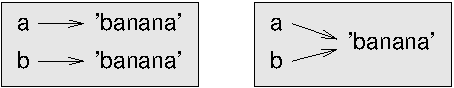
\includegraphics[scale=0.8]{figs/list1.pdf}}
\caption{State diagram.}
\label{fig.list1}
\end{figure}


In one case, {\tt a} and {\tt b} refer to two different objects that
have the same value.  In the second case, they refer to the same
object.
\index{is operator}
\index{operator!is}

To check whether two variables refer to the same object, you can
use the {\tt is} operator.

\begin{verbatim}
>>> a = 'banana'
>>> b = 'banana'
>>> a is b
True
\end{verbatim}
%
In this example, Python only created one string object,
and both {\tt a} and {\tt b} refer to it.

But when you create two lists, you get two objects:

\begin{verbatim}
>>> a = [1, 2, 3]
>>> b = [1, 2, 3]
>>> a is b
False
\end{verbatim}
%
So the state diagram looks like Figure~\ref{fig.list2}.
\index{state diagram}
\index{diagram!state}

\begin{figure}
\centerline
{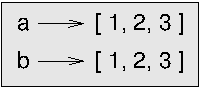
\includegraphics[scale=0.8]{figs/list2.pdf}}
\caption{State diagram.}
\label{fig.list2}
\end{figure}


In this case we would say that the two lists are {\bf equivalent},
because they have the same elements, but not {\bf identical}, because
they are not the same object.  If two objects are identical, they are
also equivalent, but if they are equivalent, they are not necessarily
identical.
\index{equivalence}
\index{identity}

Until now, we have been using ``object'' and ``value''
interchangeably, but it is more precise to say that an object has a
value.  If you execute {\tt [1,2,3]}, you get a list
object whose value is a sequence of integers.  If another
list has the same elements, we say it has the same value, but
it is not the same object.
\index{object}
\index{value}


\section{Aliasing}
\index{aliasing}
\index{reference!aliasing}

If {\tt a} refers to an object and you assign {\tt b = a},
then both variables refer to the same object:

\begin{verbatim}
>>> a = [1, 2, 3]
>>> b = a
>>> b is a
True
\end{verbatim}
%
The state diagram looks like Figure~\ref{fig.list3}.
\index{state diagram}
\index{diagram!state}

\begin{figure}
\centerline
{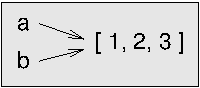
\includegraphics[scale=0.8]{figs/list3.pdf}}
\caption{State diagram.}
\label{fig.list3}
\end{figure}

The association of a variable with an object is called a {\bf
reference}.  In this example, there are two references to the same
object.
\index{reference}

An object with more than one reference has more
than one name, so we say that the object is {\bf aliased}.
\index{mutability}

If the aliased object is mutable, changes made with one alias affect
the other:

\begin{verbatim}
>>> b[0] = 17
>>> print a
[17, 2, 3]
\end{verbatim}
%
Although this behavior can be useful, it is error-prone.  In general,
it is safer to avoid aliasing when you are working with mutable
objects.
\index{immutability}

For immutable objects like strings, aliasing is not as much of a
problem.  In this example:

\begin{verbatim}
a = 'banana'
b = 'banana'
\end{verbatim}
%
It almost never makes a difference whether {\tt a} and {\tt b} refer
to the same string or not.


\section{List arguments}
\label{list.arguments}
\index{list!as argument}
\index{argument}
\index{argument!list}
\index{reference}
\index{parameter}

When you pass a list to a function, the function gets a reference
to the list.
If the function modifies a list parameter, the caller sees the change.
For example, \verb"delete_head" removes the first element from a list:

\begin{verbatim}
def delete_head(t):
    del t[0]
\end{verbatim}
%
Here's how it is used:

\begin{verbatim}
>>> letters = ['a', 'b', 'c']
>>> delete_head(letters)
>>> print letters
['b', 'c']
\end{verbatim}
%
The parameter {\tt t} and the variable {\tt letters} are
aliases for the same object.  The stack diagram looks like
Figure~\ref{fig.stack5}.
\index{stack diagram}
\index{diagram!stack}

\begin{figure}
\centerline
{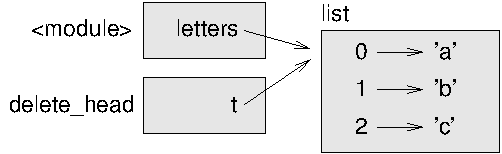
\includegraphics[scale=0.8]{figs/stack5.pdf}}
\caption{Stack diagram.}
\label{fig.stack5}
\end{figure}


Since the list is shared by two frames, I drew
it between them.

It is important to distinguish between operations that
modify lists and operations that create new lists.  For
example, the {\tt append} method modifies a list, but the
{\tt +} operator creates a new list:
\index{append method}
\index{method!append}
\index{list!concatenation}
\index{concatenation!list}

\begin{verbatim}
>>> t1 = [1, 2]
>>> t2 = t1.append(3)
>>> print t1
[1, 2, 3]
>>> print t2
None

>>> t3 = t1 + [4]
>>> print t3
[1, 2, 3, 4]
\end{verbatim}

This difference is important when you write functions that
are supposed to modify lists.  For example, this function
{\em does not} delete the head of a list:

\begin{verbatim}
def bad_delete_head(t):
    t = t[1:]              # WRONG!
\end{verbatim}

The slice operator creates a new list and the assignment
makes {\tt t} refer to it, but none of that has any effect
on the list that was passed as an argument.
\index{slice operator}
\index{operator!slice}

An alternative is to write a function that creates and
returns a new list.  For
example, {\tt tail} returns all but the first
element of a list:

\begin{verbatim}
def tail(t):
    return t[1:]
\end{verbatim}
%
This function leaves the original list unmodified.
Here's how it is used:

\begin{verbatim}
>>> letters = ['a', 'b', 'c']
>>> rest = tail(letters)
>>> print rest
['b', 'c']
\end{verbatim}



\section{Debugging}
\index{debugging}

Careless use of lists (and other mutable objects)
can lead to long hours of debugging.  Here are some common
pitfalls and ways to avoid them:

\begin{enumerate}

\item Don't forget that most list methods modify the argument and
  return {\tt None}.  This is the opposite of the string methods,
  which return a new string and leave the original alone.

If you are used to writing string code like this:

\begin{verbatim}
word = word.strip()
\end{verbatim}

It is tempting to write list code like this:

\begin{verbatim}
t = t.sort()           # WRONG!
\end{verbatim}
\index{sort method}
\index{method!sort}

Because {\tt sort} returns {\tt None}, the
next operation you perform with {\tt t} is likely to fail.

Before using list methods and operators, you should read the
documentation carefully and then test them in interactive mode.  The
methods and operators that lists share with other sequences (like
strings) are documented at
\url{http://docs.python.org/2/library/stdtypes.html#typesseq}.  The
methods and operators that only apply to mutable sequences
are documented at \url{http://docs.python.org/2/library/stdtypes.html#typesseq-mutable}.


\item Pick an idiom and stick with it.

Part of the problem with lists is that there are too many
ways to do things.  For example, to remove an element from
a list, you can use {\tt pop}, {\tt remove}, {\tt del},
or even a slice assignment.

To add an element, you can use the {\tt append} method or
the {\tt +} operator.  Assuming that {\tt t} is a list and
{\tt x} is a list element, these are right:

\begin{verbatim}
t.append(x)
t = t + [x]
\end{verbatim}

And these are wrong:

\begin{verbatim}
t.append([x])          # WRONG!
t = t.append(x)        # WRONG!
t + [x]                # WRONG!
t = t + x              # WRONG!
\end{verbatim}

Try out each of these examples in interactive mode to make sure
you understand what they do.  Notice that only the last
one causes a runtime error; the other three are legal, but they
do the wrong thing.


\item Make copies to avoid aliasing.
\index{aliasing!copying to avoid}
\index{copy!to avoid aliasing}

If you want to use a method like {\tt sort} that modifies
the argument, but you need to keep the original list as
well, you can make a copy.

\begin{verbatim}
orig = t[:]
t.sort()
\end{verbatim}

In this example you could also use the built-in function {\tt sorted},
which returns a new, sorted list and leaves the original alone.
But in that case you should avoid using {\tt sorted} as a variable
name!

\end{enumerate}



\section{Glossary}

\begin{description}

\item[list:] A sequence of values.
\index{list}

\item[element:] One of the values in a list (or other sequence),
also called items.
\index{element}

\item[index:] An integer value that indicates an element in a list.
\index{index}

\item[nested list:] A list that is an element of another list.
\index{nested list}

\item[list traversal:] The sequential accessing of each element in a list.
\index{list!traversal}

\item[mapping:] A relationship in which each element of one set
corresponds to an element of another set.  For example, a list is
a mapping from indices to elements.
\index{mapping}

\item[accumulator:] A variable used in a loop to add up or
accumulate a result.
\index{accumulator}

\item[augmented assignment:] A statement that updates the value
of a variable using an operator like \verb"+=".
\index{assignment!augmented}
\index{augmented assignment}
\index{traversal}

\item[reduce:] A processing pattern that traverses a sequence
and accumulates the elements into a single result.
\index{reduce pattern}
\index{pattern!reduce}

\item[map:] A processing pattern that traverses a sequence and
performs an operation on each element.
\index{map pattern}
\index{pattern!map}

\item[filter:] A processing pattern that traverses a list and
selects the elements that satisfy some criterion.
\index{filter pattern}
\index{pattern!filter}

\item[object:] Something a variable can refer to.  An object
has a type and a value.
\index{object}

\item[equivalent:] Having the same value.
\index{equivalent}

\item[identical:] Being the same object (which implies equivalence).
\index{identical}

\item[reference:] The association between a variable and its value.
\index{reference}

\item[aliasing:] A circumstance where two or more variables refer to the same
object.
\index{aliasing}

\item[delimiter:] A character or string used to indicate where a
string should be split.
\index{delimiter}

\end{description}


\section{Exercises}

\begin{exercise}
Write a function called \verb"is_sorted" that takes a list as a
parameter and returns {\tt True} if the list is sorted in ascending
order and {\tt False} otherwise.  You can assume (as a precondition)
that the elements of the list can be compared with the relational
operators {\tt <}, {\tt >}, etc.
\index{precondition}

For example, \verb"is_sorted([1,2,2])" should return {\tt True}
and \verb"is_sorted(['b','a'])" should return {\tt False}.
\end{exercise}


\begin{exercise}
\label{anagram}
\index{anagram}

Two words are anagrams if you can rearrange the letters from one
to spell the other.  Write a function called \verb"is_anagram"
that takes two strings and returns {\tt True} if they are anagrams.
\end{exercise}


\begin{exercise}
\label{duplicate}

The (so-called) Birthday Paradox:

\begin{enumerate}

\item Write a function called \verb"has_duplicates" that takes
a list and returns {\tt True} if there is any element that
appears more than once.  It should not modify the original
list.
\index{birthday paradox}
\index{duplicate}

\item If there are 23 students in your class, what are the chances
that two of you have the same birthday?  You can estimate this
probability by generating random samples of 23 birthdays
and checking for matches.  Hint: you can generate random birthdays
with the {\tt randint} function in the {\tt random} module.
\index{random module}
\index{module!random}
\index{randint function}
\index{function!randint}

\end{enumerate}

You can read about this problem at
\url{http://en.wikipedia.org/wiki/Birthday_paradox}, and you can download my
solution from \url{http://thinkpython.com/code/birthday.py}.

\end{exercise}


\begin{exercise}
\index{duplicate}
\index{uniqueness}

Write a function called \verb"remove_duplicates" that takes
a list and returns a new list with only the unique elements from
the original.  Hint: they don't have to be in the same order.
\end{exercise}


\begin{exercise}
\index{append method}
\index{method append}
\index{list!concatenation}
\index{concatenation!list}

Write a function that reads the file {\tt words.txt} and builds
a list with one element per word.  Write two versions of
this function, one using the {\tt append} method and the
other using the idiom {\tt t = t + [x]}.  Which one takes
longer to run?  Why?

Hint: use the {\tt time} module to measure elapsed time.
Solution: \url{http://thinkpython.com/code/wordlist.py}.
\index{time module}
\index{module!time}

\end{exercise}


\begin{exercise}
\label{wordlist1}
\label{bisection}
\index{membership!bisection search}
\index{bisection search}
\index{search, bisection}
\index{membership!binary search}
\index{binary search}
\index{search, binary}

To check whether a word is in the word list, you could use
the {\tt in} operator, but it would be slow because it searches
through the words in order.

Because the words are in alphabetical order, we can speed things up
with a bisection search (also known as binary search), which is
similar to what you do when you look a word up in the dictionary.  You
start in the middle and check to see whether the word you are looking
for comes before the word in the middle of the list.  If so, then you
search the first half of the list the same way.  Otherwise you search
the second half.

Either way, you cut the remaining search space in half.  If the
word list has 113,809 words, it will take about 17 steps to
find the word or conclude that it's not there.

Write a function called {\tt bisect} that takes a sorted list
and a target value and returns the index of the value
in the list, if it's there, or {\tt None} if it's not.
\index{bisect module}
\index{module!bisect}

Or you could read the documentation of the {\tt bisect} module
and use that!  Solution: \url{http://thinkpython.com/code/inlist.py}.

\end{exercise}

\begin{exercise}
\index{reverse word pair}

Two words are a ``reverse pair'' if each is the reverse of the
other.  Write a program that finds all the reverse pairs in the
word list.  Solution: \url{http://thinkpython.com/code/reverse_pair.py}.

\end{exercise}

\begin{exercise}
\index{interlocking words}

Two words ``interlock'' if taking alternating letters from each forms
a new word.  For example, ``shoe'' and ``cold''
interlock to form ``schooled.''
Solution: \url{http://thinkpython.com/code/interlock.py}.
Credit: This exercise is inspired by an example at \url{http://puzzlers.org}.

\begin{enumerate}

\item Write a program that finds all pairs of words that interlock.
  Hint: don't enumerate all pairs!

\item Can you find any words that are three-way interlocked; that is,
  every third letter forms a word, starting from the first, second or
  third?

\end{enumerate}
\end{exercise}


\chapter{Dictionaries}

\index{dictionary}
\index{dictionary}
\index{type!dict}
\index{key}
\index{key-value pair}
\index{index}
A {\bf dictionary} is like a list, but more general.  In a list,
the indices have to be integers; in a dictionary they can
be (almost) any type.

You can think of a dictionary as a mapping between a set of indices
(which are called {\bf keys}) and a set of values.  Each key maps to a
value.  The association of a key and a value is called a {\bf
  key-value pair} or sometimes an {\bf item}.

As an example, we'll build a dictionary that maps from English
to Spanish words, so the keys and the values are all strings.

The function {\tt dict} creates a new dictionary with no items.
Because {\tt dict} is the name of a built-in function, you
should avoid using it as a variable name.
\index{dict function}
\index{function!dict}

\begin{verbatim}
>>> eng2sp = dict()
>>> print eng2sp
{}
\end{verbatim}

The squiggly-brackets, \verb"{}", represent an empty dictionary.
To add items to the dictionary, you can use square brackets:
\index{squiggly bracket}
\index{bracket!squiggly}

\begin{verbatim}
>>> eng2sp['one'] = 'uno'
\end{verbatim}
%
This line creates an item that maps from the key
{\tt 'one'} to the value \verb"'uno'".  If we print the
dictionary again, we see a key-value pair with a colon
between the key and value:

\begin{verbatim}
>>> print eng2sp
{'one': 'uno'}
\end{verbatim}
%
This output format is also an input format.  For example,
you can create a new dictionary with three items:

\begin{verbatim}
>>> eng2sp = {'one': 'uno', 'two': 'dos', 'three': 'tres'}
\end{verbatim}
%
But if you print {\tt eng2sp}, you might be surprised:

\begin{verbatim}
>>> print eng2sp
{'one': 'uno', 'three': 'tres', 'two': 'dos'}
\end{verbatim}
%
The order of the key-value pairs is not the same.  In fact, if
you type the same example on your computer, you might get a
different result.  In general, the order of items in
a dictionary is unpredictable.

But that's not a problem because
the elements of a dictionary are never indexed with integer indices.
Instead, you use the keys to look up the corresponding values:

\begin{verbatim}
>>> print eng2sp['two']
'dos'
\end{verbatim}
%
The key {\tt 'two'} always maps to the value \verb"'dos'" so the order
of the items doesn't matter.

If the key isn't in the dictionary, you get an exception:
\index{exception!KeyError}
\index{KeyError}

\begin{verbatim}
>>> print eng2sp['four']
KeyError: 'four'
\end{verbatim}
%
The {\tt len} function works on dictionaries; it returns the
number of key-value pairs:
\index{len function}
\index{function!len}

\begin{verbatim}
>>> len(eng2sp)
3
\end{verbatim}
%
The {\tt in} operator works on dictionaries; it tells you whether
something appears as a {\em key} in the dictionary (appearing
as a value is not good enough).
\index{membership!dictionary}
\index{in operator}
\index{operator!in}

\begin{verbatim}
>>> 'one' in eng2sp
True
>>> 'uno' in eng2sp
False
\end{verbatim}
%
To see whether something appears as a value in a dictionary, you
can use the method {\tt values}, which returns the values as
a list, and then use the {\tt in} operator:
\index{values method}
\index{method!values}

\begin{verbatim}
>>> vals = eng2sp.values()
>>> 'uno' in vals
True
\end{verbatim}
%
The {\tt in} operator uses different algorithms for lists and
dictionaries.  For lists, it uses a search algorithm, as in
Section~\ref{find}.  As the list gets longer, the search time gets
longer in direct proportion.  For dictionaries, Python uses an
algorithm called a {\bf hashtable} that has a remarkable property: the
{\tt in} operator takes about the same amount of time no matter how
many items there are in a dictionary.  I won't explain how that's
possible, but you can read more about it at
\url{http://en.wikipedia.org/wiki/Hash_table}.
\index{hashtable}

\begin{exercise}
\label{wordlist2}
\index{set membership}
\index{membership!set}

Write a function that reads the words in {\tt words.txt} and
stores them as keys in a dictionary.  It doesn't matter what the
values are.  Then you can use the {\tt in} operator
as a fast way to check whether a string is in
the dictionary.

If you did Exercise~\ref{wordlist1}, you can compare the speed
of this implementation with the list {\tt in} operator and the
bisection search.

\end{exercise}


\section{Dictionary as a set of counters}
\label{histogram}
\index{counter}

Suppose you are given a string and you want to count how many
times each letter appears.  There are several ways you could do it:

\begin{enumerate}

\item You could create 26 variables, one for each letter of the
alphabet.  Then you could traverse the string and, for each
character, increment the corresponding counter, probably using
a chained conditional.

\item You could create a list with 26 elements.  Then you could
convert each character to a number (using the built-in function
{\tt ord}), use the number as an index into the list, and increment
the appropriate counter.

\item You could create a dictionary with characters as keys
and counters as the corresponding values.  The first time you
see a character, you would add an item to the dictionary.  After
that you would increment the value of an existing item.

\end{enumerate}

Each of these options performs the same computation, but each
of them implements that computation in a different way.
\index{implementation}

An {\bf implementation} is a way of performing a computation;
some implementations are better than others.  For example,
an advantage of the dictionary implementation is that we don't
have to know ahead of time which letters appear in the string
and we only have to make room for the letters that do appear.

Here is what the code might look like:

\begin{verbatim}
def histogram(s):
    d = dict()
    for c in s:
        if c not in d:
            d[c] = 1
        else:
            d[c] += 1
    return d
\end{verbatim}
%
The name of the function is {\bf histogram}, which is a statistical
term for a set of counters (or frequencies).
\index{histogram}
\index{frequency}
\index{traversal}

The first line of the
function creates an empty dictionary.  The {\tt for} loop traverses
the string.  Each time through the loop, if the character {\tt c} is
not in the dictionary, we create a new item with key {\tt c} and the
initial value 1 (since we have seen this letter once).  If {\tt c} is
already in the dictionary we increment {\tt d[c]}.
\index{histogram}

Here's how it works:

\begin{verbatim}
>>> h = histogram('brontosaurus')
>>> print h
{'a': 1, 'b': 1, 'o': 2, 'n': 1, 's': 2, 'r': 2, 'u': 2, 't': 1}
\end{verbatim}
%
The histogram indicates that the letters {\tt 'a'} and \verb"'b'"
appear once; \verb"'o'" appears twice, and so on.

\begin{exercise}
\index{get method}
\index{method!get}

Dictionaries have a method called {\tt get} that takes a key
and a default value.  If the key appears in the dictionary,
{\tt get} returns the corresponding value; otherwise it returns
the default value.  For example:

\begin{verbatim}
>>> h = histogram('a')
>>> print h
{'a': 1}
>>> h.get('a', 0)
1
>>> h.get('b', 0)
0
\end{verbatim}
%
Use {\tt get} to write {\tt histogram} more concisely.  You
should be able to eliminate the {\tt if} statement.
\end{exercise}


\section{Looping and dictionaries}
\index{dictionary!looping with}
\index{looping!with dictionaries}
\index{traversal}

If you use a dictionary in a {\tt for} statement, it traverses
the keys of the dictionary.  For example, \verb"print_hist"
prints each key and the corresponding value:

\begin{verbatim}
def print_hist(h):
    for c in h:
        print c, h[c]
\end{verbatim}
%
Here's what the output looks like:

\begin{verbatim}
>>> h = histogram('parrot')
>>> print_hist(h)
a 1
p 1
r 2
t 1
o 1
\end{verbatim}
%
Again, the keys are in no particular order.

\begin{exercise}
\index{keys method}
\index{method!keys}

Dictionaries have a method called {\tt keys} that returns
the keys of the dictionary, in no particular order, as a list.

Modify \verb"print_hist" to print the keys and their values
in alphabetical order.
\end{exercise}



\section{Reverse lookup}
\label{raise}
\index{dictionary!lookup}
\index{dictionary!reverse lookup}
\index{lookup, dictionary}
\index{reverse lookup, dictionary}

Given a dictionary {\tt d} and a key {\tt k}, it is easy to
find the corresponding value {\tt v = d[k]}.  This operation
is called a {\bf lookup}.

But what if you have {\tt v} and you want to find {\tt k}?
You have two problems: first, there might be more than one
key that maps to the value {\tt v}.  Depending on the application,
you might be able to pick one, or you might have to make
a list that contains all of them.  Second, there is no
simple syntax to do a {\bf reverse lookup}; you have to search.

Here is a function that takes a value and returns the first
key that maps to that value:

\begin{verbatim}
def reverse_lookup(d, v):
    for k in d:
        if d[k] == v:
            return k
    raise ValueError
\end{verbatim}
%
This function is yet another example of the search pattern, but it
uses a feature we haven't seen before, {\tt raise}.  The {\tt raise}
statement causes an exception; in this case it causes a {\tt
  ValueError}, which generally indicates that there is something wrong
with the value of a parameter.
\index{search}
\index{pattern!search}
\index{raise statement}
\index{statement!raise}
\index{exception!ValueError}
\index{ValueError}

If we get to the end of the loop, that means {\tt v}
doesn't appear in the dictionary as a value, so we raise an
exception.

Here is an example of a successful reverse lookup:

\begin{verbatim}
>>> h = histogram('parrot')
>>> k = reverse_lookup(h, 2)
>>> print k
r
\end{verbatim}
%
And an unsuccessful one:

\begin{verbatim}
>>> k = reverse_lookup(h, 3)
Traceback (most recent call last):
  File "<stdin>", line 1, in ?
  File "<stdin>", line 5, in reverse_lookup
ValueError
\end{verbatim}
%
The result when you raise an exception is the same as when
Python raises one: it prints a traceback and an error message.
\index{traceback}
\index{optional argument}
\index{argument!optional}

The {\tt raise} statement takes a detailed error message as an
optional argument.  For example:

\begin{verbatim}
>>> raise ValueError, 'value does not appear in the dictionary'
Traceback (most recent call last):
  File "<stdin>", line 1, in ?
ValueError: value does not appear in the dictionary
\end{verbatim}
%
A reverse lookup is much slower than a forward lookup; if you
have to do it often, or if the dictionary gets big, the performance
of your program will suffer.

\begin{exercise}

Modify \verb"reverse_lookup" so that it builds and returns a list
of {\em all} keys that map to {\tt v}, or an empty list if there
are none.

\end{exercise}


\section{Dictionaries and lists}
\label{invert}

Lists can appear as values in a dictionary.  For example, if you
were given a dictionary that maps from letters to frequencies, you
might want to invert it; that is, create a dictionary that maps
from frequencies to letters.  Since there might be several letters
with the same frequency, each value in the inverted dictionary
should be a list of letters.
\index{invert dictionary}
\index{dictionary!invert}

Here is a function that inverts a dictionary:

\begin{verbatim}
def invert_dict(d):
    inverse = dict()
    for key in d:
        val = d[key]
        if val not in inverse:
            inverse[val] = [key]
        else:
            inverse[val].append(key)
    return inverse
\end{verbatim}
%
Each time through the loop, {\tt key} gets a key from {\tt d} and
{\tt val} gets the corresponding value.  If {\tt val} is not in {\tt inverse},
that means we haven't seen it before, so we create a new item and
initialize it with a {\bf singleton} (a list that contains a
single element).  Otherwise we have seen this value before, so we
append the corresponding key to the list.
\index{singleton}

Here is an example:

\begin{verbatim}
>>> hist = histogram('parrot')
>>> print hist
{'a': 1, 'p': 1, 'r': 2, 't': 1, 'o': 1}
>>> inverse = invert_dict(hist)
>>> print inverse
{1: ['a', 'p', 't', 'o'], 2: ['r']}
\end{verbatim}

\begin{figure}
\centerline
{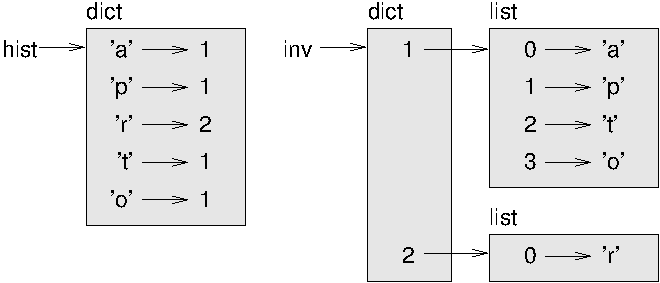
\includegraphics[scale=0.8]{figs/dict1.pdf}}
\caption{State diagram.}
\label{fig.dict1}
\end{figure}

Figure~\ref{fig.dict1} is a state diagram showing {\tt hist} and {\tt inverse}.
A dictionary is represented as a box with the type {\tt dict} above it
and the key-value pairs inside.  If the values are integers, floats or
strings, I usually draw them inside the box, but I usually draw lists
outside the box, just to keep the diagram simple.
\index{state diagram}
\index{diagram!state}

Lists can be values in a dictionary, as this example shows, but they
cannot be keys.  Here's what happens if you try:
\index{TypeError}
\index{exception!TypeError}


\begin{verbatim}
>>> t = [1, 2, 3]
>>> d = dict()
>>> d[t] = 'oops'
Traceback (most recent call last):
  File "<stdin>", line 1, in ?
TypeError: list objects are unhashable
\end{verbatim}
%
I mentioned earlier that a dictionary is implemented using
a hashtable and that means that the keys have to be {\bf hashable}.
\index{hash function}
\index{hashable}

A {\bf hash} is a function that takes a value (of any kind)
and returns an integer.  Dictionaries use these integers,
called hash values, to store and look up key-value pairs.
\index{immutability}

This system works fine if the keys are immutable.  But if the
keys are mutable, like lists, bad things happen.  For example,
when you create a key-value pair, Python hashes the key and
stores it in the corresponding location.  If you modify the
key and then hash it again, it would go to a different location.
In that case you might have two entries for the same key,
or you might not be able to find a key.  Either way, the
dictionary wouldn't work correctly.

That's why the keys have to be hashable, and why mutable types like
lists aren't.  The simplest way to get around this limitation is to
use tuples, which we will see in the next chapter.

Since dictionaries are mutable, they can't be used as keys,
but they {\em can} be used as values.

\begin{exercise}
Read the documentation of the dictionary method {\tt setdefault}
and use it to write a more concise version of \verb"invert_dict".
Solution: \url{http://thinkpython.com/code/invert_dict.py}.
\index{setdefault method}
\index{method!setdefault}

\end{exercise}


\section{Memos}

If you played with the {\tt fibonacci} function from
Section~\ref{one.more.example}, you might have noticed that the bigger
the argument you provide, the longer the function takes to run.
Furthermore, the run time increases very quickly.
\index{fibonacci function}
\index{function!fibonacci}

To understand why, consider Figure~\ref{fig.fibonacci}, which shows
the {\bf call graph} for {\tt fibonacci} with {\tt n=4}:

\begin{figure}
\centerline
{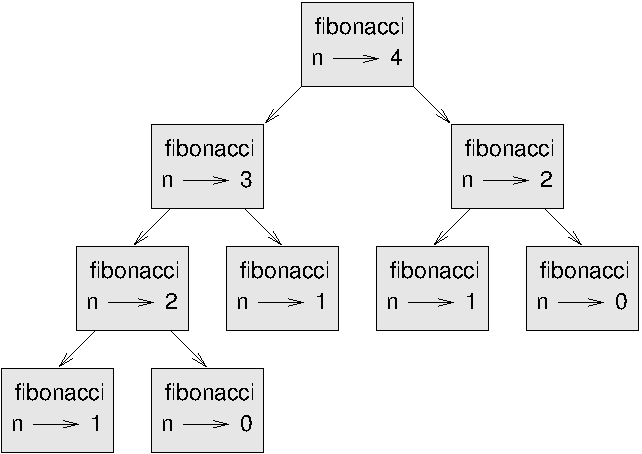
\includegraphics[scale=0.7]{figs/fibonacci.pdf}}
\caption{Call graph.}
\label{fig.fibonacci}
\end{figure}

A call graph shows a set of function frames, with lines connecting each
frame to the frames of the functions it calls.  At the top of the
graph, {\tt fibonacci} with {\tt n=4} calls {\tt fibonacci} with {\tt
n=3} and {\tt n=2}.  In turn, {\tt fibonacci} with {\tt n=3} calls
{\tt fibonacci} with {\tt n=2} and {\tt n=1}.  And so on.
\index{function frame}
\index{frame}
\index{call graph}

Count how many times {\tt fibonacci(0)} and {\tt fibonacci(1)} are
called.  This is an inefficient solution to the problem, and it gets
worse as the argument gets bigger.
\index{memo}

One solution is to keep track of values that have already been
computed by storing them in a dictionary.  A previously computed value
that is stored for later use is called a {\bf memo}.  Here is an
implementation of {\tt fibonacci} using memos:

\begin{verbatim}
known = {0:0, 1:1}

def fibonacci(n):
    if n in known:
        return known[n]

    res = fibonacci(n-1) + fibonacci(n-2)
    known[n] = res
    return res
\end{verbatim}
%
{\tt known} is a dictionary that keeps track of the Fibonacci
numbers we already know.  It starts with
two items: 0 maps to 0 and 1 maps to 1.

Whenever {\tt fibonacci} is called, it checks {\tt known}.
If the result is already there, it can return
immediately.  Otherwise it has to
compute the new value, add it to the dictionary, and return it.

\begin{exercise}

Run this version of {\tt fibonacci} and the original with
a range of parameters and compare their run times.

\end{exercise}

\begin{exercise}

Memoize the Ackermann function from Exercise~\ref{ackermann} and see if
memoization makes it possible to evaluate the function with bigger
arguments.  Hint: no.
Solution: \url{http://thinkpython.com/code/ackermann_memo.py}.
\index{Ackermann function}
\index{function!ack}

\end{exercise}


\section{Global variables}
\index{global variable}
\index{variable!global}

In the previous example, {\tt known} is created outside the function,
so it belongs to the special frame called \verb"__main__".
Variables in \verb"__main__" are sometimes called {\bf global}
because they can be accessed from any function.  Unlike local
variables, which disappear when their function ends, global variables
persist from one function call to the next.
\index{flag}

It is common to use global variables for {\bf flags}; that is,
boolean variables that indicate (``flag'') whether a condition
is true.  For example, some programs use
a flag named {\tt verbose} to control the level of detail in the
output:

\begin{verbatim}
verbose = True

def example1():
    if verbose:
        print 'Running example1'
\end{verbatim}
%
If you try to reassign a global variable, you might be surprised.
The following example is supposed to keep track of whether the
function has been called:
\index{multiple assignment}
\index{assignment!multiple}

\begin{verbatim}
been_called = False

def example2():
    been_called = True         # WRONG
\end{verbatim}
%
But if you run it you will see that the value of \verb"been_called"
doesn't change.  The problem is that {\tt example2} creates a new local
variable named \verb"been_called".  The local variable goes away when
the function ends, and has no effect on the global variable.
\index{global statement}
\index{statement!global}
\index{declaration}

To reassign a global variable inside a function you have to
{\bf declare} the global variable before you use it:

\begin{verbatim}
been_called = False

def example2():
    global been_called
    been_called = True
\end{verbatim}
%
The {\tt global} statement tells the interpreter
something like, ``In this function, when I say \verb"been_called", I
mean the global variable; don't create a local one.''
\index{update!global variable}
\index{global variable!update}

Here's an example that tries to update a global variable:

\begin{verbatim}
count = 0

def example3():
    count = count + 1          # WRONG
\end{verbatim}
%
If you run it you get:
\index{UnboundLocalError}
\index{exception!UnboundLocalError}

\begin{verbatim}
UnboundLocalError: local variable 'count' referenced before assignment
\end{verbatim}
%
Python assumes that {\tt count} is local, which means
that you are reading it before writing it.  The solution, again,
is to declare {\tt count} global.
\index{counter}

\begin{verbatim}
def example3():
    global count
    count += 1
\end{verbatim}
%
If the global value is mutable, you can modify it without
declaring it:
\index{mutability}

\begin{verbatim}
known = {0:0, 1:1}

def example4():
    known[2] = 1
\end{verbatim}
%
So you can add, remove and replace elements of a global list or
dictionary, but if you want to reassign the variable, you
have to declare it:

\begin{verbatim}
def example5():
    global known
    known = dict()
\end{verbatim}
%

\section{Long integers}
\index{long integer}
\index{integer!long}
\index{type!long}

If you compute {\tt fibonacci(50)}, you get:

\begin{verbatim}
>>> fibonacci(50)
12586269025L
\end{verbatim}
%
The {\tt L} at the end indicates that the result is a long
integer, or type {\tt long}.  In Python 3, {\tt long} is gone; all integers,
even really big ones, are type {\tt int}.
\index{Python 3}

Values with type {\tt int} have a limited range;
long integers can be arbitrarily big, but as they get bigger
they consume more space and time.

The mathematical operators work on long integers, and the functions
in the {\tt math} module, too, so in general any code that
works with {\tt int} will also work with {\tt long}.

Any time the result of a computation is too big to be represented with
an integer, Python converts the result as a long integer:

\begin{verbatim}
>>> 1000 * 1000
1000000
>>> 100000 * 100000
10000000000L
\end{verbatim}
%
In the first case the result has type {\tt int}; in the
second case it is {\tt long}.

\begin{exercise}
\index{encryption}
\index{RSA algorithm}
\index{algorithm!RSA}

Exponentiation of large integers is the basis of common
algorithms for public-key encryption.  Read the Wikipedia
page on the RSA algorithm (\url{http://en.wikipedia.org/wiki/RSA})
and write functions to encode and decode messages.

% TODO: solution for this one!

\end{exercise}


\section{Debugging}
\index{debugging}

As you work with bigger datasets it can become unwieldy to
debug by printing and checking data by hand.  Here are some
suggestions for debugging large datasets:

\begin{description}

\item[Scale down the input:] If possible, reduce the size of the
dataset.  For example if the program reads a text file, start with
just the first 10 lines, or with the smallest example you can find.
You can either edit the files themselves, or (better) modify the
program so it reads only the first {\tt n} lines.

If there is an error, you can reduce {\tt n} to the smallest
value that manifests the error, and then increase it gradually
as you find and correct errors.

\item[Check summaries and types:] Instead of printing and checking the
entire dataset, consider printing summaries of the data: for example,
the number of items in a dictionary or the total of a list of numbers.

A common cause of runtime errors is a value that is not the right
type.  For debugging this kind of error, it is often enough to print
the type of a value.

\item[Write self-checks:]  Sometimes you can write code to check
for errors automatically.  For example, if you are computing the
average of a list of numbers, you could check that the result is
not greater than the largest element in the list or less than
the smallest.  This is called a ``sanity check'' because it detects
results that are ``insane.''
\index{sanity check}
\index{consistency check}

Another kind of check compares the results of two different
computations to see if they are consistent.  This is called a
``consistency check.''

\item[Pretty print the output:] Formatting debugging output
can make it easier to spot an error.  We saw an example in
Section~\ref{factdebug}.  The {\tt pprint} module provides
a {\tt pprint} function that displays built-in types in
a more human-readable format.
\index{pretty print}
\index{pprint module}
\index{module!pprint}

\end{description}

Again, time you spend building scaffolding can reduce
the time you spend debugging.
\index{scaffolding}

\section{Glossary}

\begin{description}

\item[dictionary:] A mapping from a set of keys to their
corresponding values.
\index{dictionary}

\item[key-value pair:] The representation of the mapping from
a key to a value.
\index{key-value pair}

\item[item:] Another name for a key-value pair.
\index{item!dictionary}

\item[key:] An object that appears in a dictionary as the
first part of a key-value pair.
\index{key}

\item[value:] An object that appears in a dictionary as the
second part of a key-value pair.  This is more specific than
our previous use of the word ``value.''
\index{value}

\item[implementation:] A way of performing a computation.
\index{implementation}

\item[hashtable:] The algorithm used to implement Python
dictionaries.
\index{hashtable}

\item[hash function:] A function used by a hashtable to compute the
location for a key.
\index{hash function}

\item[hashable:] A type that has a hash function.  Immutable
types like integers,
floats and strings are hashable; mutable types like lists and
dictionaries are not.
\index{hashable}

\item[lookup:] A dictionary operation that takes a key and finds
the corresponding value.
\index{lookup}

\item[reverse lookup:] A dictionary operation that takes a value and finds
one or more keys that map to it.
\index{reverse lookup, dictionary}

\item[singleton:] A list (or other sequence) with a single element.
\index{singleton}

\item[call graph:] A diagram that shows every frame created during
the execution of a program, with an arrow from each caller to
each callee.
\index{call graph}
\index{diagram!call graph}

\item[histogram:] A set of counters.
\index{histogram}

\item[memo:] A computed value stored to avoid unnecessary future
computation.
\index{memo}

\item[global variable:]  A variable defined outside a function.  Global
variables can be accessed from any function.
\index{global variable}

\item[flag:] A boolean variable used to indicate whether a condition
is true.
\index{flag}

\item[declaration:] A statement like {\tt global} that tells the
interpreter something about a variable.
\index{declaration}

\end{description}

\section{Exercises}

\begin{exercise}
\index{duplicate}

If you did Exercise~\ref{duplicate}, you already have
a function named \verb"has_duplicates" that takes a list
as a parameter and returns {\tt True} if there is any object
that appears more than once in the list.

Use a dictionary to write a faster, simpler version of
\verb"has_duplicates".
Solution: \url{http://thinkpython.com/code/has_duplicates.py}.

\end{exercise}


\begin{exercise}
\label{exrotatepairs}
\index{letter rotation}
\index{rotation!letters}

Two words are ``rotate pairs'' if you can rotate one of them
and get the other (see \verb"rotate_word" in Exercise~\ref{exrotate}).

Write a program that reads a wordlist and finds all the rotate
pairs.  Solution: \url{http://thinkpython.com/code/rotate_pairs.py}.

\end{exercise}


\begin{exercise}
\index{Car Talk}
\index{Puzzler}

Here's another Puzzler from {\em Car
Talk} (\url{http://www.cartalk.com/content/puzzlers}):

\begin{quote}
This was sent in by a fellow named Dan O'Leary. He came upon a common
one-syllable, five-letter word recently that has the following unique
property. When you remove the first letter, the remaining letters form
a homophone of the original word, that is a word that sounds exactly
the same. Replace the first letter, that is, put it back and remove
the second letter and the result is yet another homophone of the
original word. And the question is, what's the word?

Now I'm going to give you an example that doesn't work. Let's look at
the five-letter word, `wrack.' W-R-A-C-K, you know like to `wrack with
pain.' If I remove the first letter, I am left with a four-letter
word, 'R-A-C-K.' As in, `Holy cow, did you see the rack on that buck!
It must have been a nine-pointer!' It's a perfect homophone. If you
put the `w' back, and remove the `r,' instead, you're left with the
word, `wack,' which is a real word, it's just not a homophone of the
other two words.

But there is, however, at least one word that Dan and we know of,
which will yield two homophones if you remove either of the first two
letters to make two, new four-letter words. The question is, what's
the word?
\end{quote}
\index{homophone}
\index{reducible word}
\index{word, reducible}

You can use the dictionary from Exercise~\ref{wordlist2} to check
whether a string is in the word list.

To check whether two words are homophones, you can use the CMU
Pronouncing Dictionary.  You can download it from
\url{http://www.speech.cs.cmu.edu/cgi-bin/cmudict} or from
\url{http://thinkpython.com/code/c06d} and you can also download
\url{http://thinkpython.com/code/pronounce.py}, which provides a function
named \verb"read_dictionary" that reads the pronouncing dictionary and
returns a Python dictionary that maps from each word to a string that
describes its primary pronunciation.

Write a program that lists all the words that solve the Puzzler.
Solution: \url{http://thinkpython.com/code/homophone.py}.

\end{exercise}



\chapter{Tuples}
\label{tuplechap}

\section{Tuples are immutable}
\index{tuple}
\index{type!tuple}
\index{sequence}

A tuple is a sequence of values.  The values can be any type, and
they are indexed by integers, so in that respect tuples are a lot
like lists.  The important difference is that tuples are immutable.
\index{mutability}
\index{immutability}

Syntactically, a tuple is a comma-separated list of values:

\begin{verbatim}
>>> t = 'a', 'b', 'c', 'd', 'e'
\end{verbatim}
%
Although it is not necessary, it is common to enclose tuples in
parentheses:
\index{parentheses!tuples in}

\begin{verbatim}
>>> t = ('a', 'b', 'c', 'd', 'e')
\end{verbatim}
%
To create a tuple with a single element, you have to include a final
comma:
\index{singleton}
\index{tuple!singleton}

\begin{verbatim}
>>> t1 = 'a',
>>> type(t1)
<type 'tuple'>
\end{verbatim}
%
A value in parentheses is not a tuple:

\begin{verbatim}
>>> t2 = ('a')
>>> type(t2)
<type 'str'>
\end{verbatim}
%
Another way to create a tuple is the built-in function {\tt tuple}.
With no argument, it creates an empty tuple:
\index{tuple function}
\index{function!tuple}

\begin{verbatim}
>>> t = tuple()
>>> print t
()
\end{verbatim}
%
If the argument is a sequence (string, list or tuple), the result
is a tuple with the elements of the sequence:

\begin{verbatim}
>>> t = tuple('lupins')
>>> print t
('l', 'u', 'p', 'i', 'n', 's')
\end{verbatim}
%
Because {\tt tuple} is the name of a built-in function, you should
avoid using it as a variable name.

Most list operators also work on tuples.  The bracket operator
indexes an element:
\index{bracket operator}
\index{operator!bracket}

\begin{verbatim}
>>> t = ('a', 'b', 'c', 'd', 'e')
>>> print t[0]
'a'
\end{verbatim}
%
And the slice operator selects a range of elements.
\index{slice operator}
\index{operator!slice}
\index{tuple!slice}
\index{slice!tuple}

\begin{verbatim}
>>> print t[1:3]
('b', 'c')
\end{verbatim}
%
But if you try to modify one of the elements of the tuple, you get
an error:
\index{exception!TypeError}
\index{TypeError}
\index{item assignment}
\index{assignment!item}

\begin{verbatim}
>>> t[0] = 'A'
TypeError: object doesn't support item assignment
\end{verbatim}
%
You can't modify the elements of a tuple, but you can replace
one tuple with another:

\begin{verbatim}
>>> t = ('A',) + t[1:]
>>> print t
('A', 'b', 'c', 'd', 'e')
\end{verbatim}
%

\section{Tuple assignment}
\label{tuple.assignment}
\index{tuple!assignment}
\index{assignment!tuple}
\index{swap pattern}
\index{pattern!swap}

It is often useful to swap the values of two variables.
With conventional assignments, you have to use a temporary
variable.  For example, to swap {\tt a} and {\tt b}:

\begin{verbatim}
>>> temp = a
>>> a = b
>>> b = temp
\end{verbatim}
%
This solution is cumbersome; {\bf tuple assignment} is more elegant:

\begin{verbatim}
>>> a, b = b, a
\end{verbatim}
%
The left side is a tuple of variables; the right side is a tuple of
expressions.  Each value is assigned to its respective variable.
All the expressions on the right side are evaluated before any
of the assignments.

The number of variables on the left and the number of
values on the right have to be the same:
\index{exception!ValueError}
\index{ValueError}

\begin{verbatim}
>>> a, b = 1, 2, 3
ValueError: too many values to unpack
\end{verbatim}
%
More generally, the right side can be any kind of sequence
(string, list or tuple).  For example, to split an email address
into a user name and a domain, you could write:
\index{split method}
\index{method!split}
\index{email address}

\begin{verbatim}
>>> addr = 'monty@python.org'
>>> uname, domain = addr.split('@')
\end{verbatim}
%
The return value from {\tt split} is a list with two elements;
the first element is assigned to {\tt uname}, the second to
{\tt domain}.

\begin{verbatim}
>>> print uname
monty
>>> print domain
python.org
\end{verbatim}
%

\section{Tuples as return values}
\index{tuple}
\index{value!tuple}
\index{return value!tuple}
\index{function, tuple as return value}

Strictly speaking, a function can only return one value, but
if the value is a tuple, the effect is the same as returning
multiple values.  For example, if you want to divide two integers
and compute the quotient and remainder, it is inefficient to
compute {\tt x/y} and then {\tt x\%y}.  It is better to compute
them both at the same time.
\index{divmod}

The built-in function {\tt divmod} takes two arguments and
returns a tuple of two values, the quotient and remainder.
You can store the result as a tuple:

\begin{verbatim}
>>> t = divmod(7, 3)
>>> print t
(2, 1)
\end{verbatim}
%
Or use tuple assignment to store the elements separately:
\index{tuple assignment}
\index{assignment!tuple}

\begin{verbatim}
>>> quot, rem = divmod(7, 3)
>>> print quot
2
>>> print rem
1
\end{verbatim}
%
Here is an example of a function that returns a tuple:

\begin{verbatim}
def min_max(t):
    return min(t), max(t)
\end{verbatim}
%
{\tt max} and {\tt min} are built-in functions that find
the largest and smallest elements of a sequence.  \verb"min_max"
computes both and returns a tuple of two values.
\index{max function}
\index{function!max}
\index{min function}
\index{function!min}


\section{Variable-length argument tuples}
\index{variable-length argument tuple}
\index{argument!variable-length tuple}
\index{gather}
\index{parameter!gather}
\index{argument!gather}

Functions can take a variable number of arguments.  A parameter
name that begins with {\tt *} {\bf gathers} arguments into
a tuple.  For example, {\tt printall}
takes any number of arguments and prints them:

\begin{verbatim}
def printall(*args):
    print args
\end{verbatim}
%
The gather parameter can have any name you like, but {\tt args} is
conventional.  Here's how the function works:

\begin{verbatim}
>>> printall(1, 2.0, '3')
(1, 2.0, '3')
\end{verbatim}
%
The complement of gather is {\bf scatter}.  If you have a
sequence of values and you want to pass it to a function
as multiple arguments, you can use the {\tt *} operator.
For example, {\tt divmod} takes exactly two arguments; it
doesn't work with a tuple:

% removing this because we haven't seen optional parameters yet
%You can combine the gather operator with required and positional
%arguments:

%%\begin{verbatim}
%def pointless(required, optional=0, *args):
%    print required, optional, args
%\end{verbatim}
%\afterverb
%
%Run this function with 1, 2, 3 and 4 or more arguments and
%make sure you understand what it does.
\index{scatter}
\index{argument scatter}
\index{TypeError}
\index{exception!TypeError}

\begin{verbatim}
>>> t = (7, 3)
>>> divmod(t)
TypeError: divmod expected 2 arguments, got 1
\end{verbatim}
%
But if you scatter the tuple, it works:

\begin{verbatim}
>>> divmod(*t)
(2, 1)
\end{verbatim}
%
\begin{exercise}

Many of the built-in functions use
variable-length argument tuples.  For example, {\tt max}
and {\tt min} can take any number of arguments:
\index{max function}
\index{function!max}
\index{min function}
\index{function!min}

\begin{verbatim}
>>> max(1,2,3)
3
\end{verbatim}
%
But {\tt sum} does not.
\index{sum function}
\index{function!sum}

\begin{verbatim}
>>> sum(1,2,3)
TypeError: sum expected at most 2 arguments, got 3
\end{verbatim}
%
Write a function called {\tt sumall} that takes any number
of arguments and returns their sum.

\end{exercise}


\section{Lists and tuples}
\index{zip function}
\index{function!zip}

{\tt zip} is a built-in function that takes two or more sequences and
``zips'' them into a list of tuples where each tuple contains one
element from each sequence.  In Python 3, {\tt zip} returns an iterator
of tuples, but for most purposes, an iterator behaves like a list.
\index{Python 3}

This example zips a string and a list:

\begin{verbatim}
>>> s = 'abc'
>>> t = [0, 1, 2]
>>> zip(s, t)
[('a', 0), ('b', 1), ('c', 2)]
\end{verbatim}
%
The result is a list of tuples where each tuple contains
a character from the string and the corresponding element from
the list.
\index{list!of tuples}

If the sequences are not the same length, the result has the
length of the shorter one.

\begin{verbatim}
>>> zip('Anne', 'Elk')
[('A', 'E'), ('n', 'l'), ('n', 'k')]
\end{verbatim}
%
You can use tuple assignment in a {\tt for} loop to traverse a list of
tuples:
\index{traversal}
\index{tuple assignment}
\index{assignment!tuple}

\begin{verbatim}
t = [('a', 0), ('b', 1), ('c', 2)]
for letter, number in t:
    print number, letter
\end{verbatim}
%
Each time through the loop, Python selects the next tuple in
the list and assigns the elements to {\tt letter} and
{\tt number}.  The output of this loop is:
\index{loop}

\begin{verbatim}
0 a
1 b
2 c
\end{verbatim}
%
If you combine {\tt zip}, {\tt for} and tuple assignment, you get a
useful idiom for traversing two (or more) sequences at the same
time.  For example, \verb"has_match" takes two sequences, {\tt t1} and
{\tt t2}, and returns {\tt True} if there is an index {\tt i}
such that {\tt t1[i] == t2[i]}:
\index{for loop}

\begin{verbatim}
def has_match(t1, t2):
    for x, y in zip(t1, t2):
        if x == y:
            return True
    return False
\end{verbatim}
%
If you need to traverse the elements of a sequence and their
indices, you can use the built-in function {\tt enumerate}:
\index{traversal}
\index{enumerate function}
\index{function!enumerate}

\begin{verbatim}
for index, element in enumerate('abc'):
    print index, element
\end{verbatim}
%
The output of this loop is:

\begin{verbatim}
0 a
1 b
2 c
\end{verbatim}
%
Again.


\section{Dictionaries and tuples}
\label{dictuple}
\index{dictionary}
\index{items method}
\index{method!items}
\index{key-value pair}

Dictionaries have a method called {\tt items} that returns a list of
tuples, where each tuple is a key-value pair.

\begin{verbatim}
>>> d = {'a':0, 'b':1, 'c':2}
>>> t = d.items()
>>> print t
[('a', 0), ('c', 2), ('b', 1)]
\end{verbatim}
%
As you should expect from a dictionary, the items are in no
particular order.  In Python 3, {\tt items} returns an iterator,
but for many purposes, iterators behave like lists.

Going in the other direction, you can use a list of tuples to
initialize a new dictionary: \index{dictionary!initialize}

\begin{verbatim}
>>> t = [('a', 0), ('c', 2), ('b', 1)]
>>> d = dict(t)
>>> print d
{'a': 0, 'c': 2, 'b': 1}
\end{verbatim}

Combining {\tt dict} with {\tt zip} yields a concise way
to create a dictionary:
\index{zip function!use with dict}

\begin{verbatim}
>>> d = dict(zip('abc', range(3)))
>>> print d
{'a': 0, 'c': 2, 'b': 1}
\end{verbatim}
%
The dictionary method {\tt update} also takes a list of tuples
and adds them, as key-value pairs, to an existing dictionary.
\index{update method}
\index{method!update}
\index{traverse!dictionary}
\index{dictionary!traversal}

Combining {\tt items}, tuple assignment and {\tt for}, you
get the idiom for traversing the keys and values of a dictionary:

\begin{verbatim}
for key, val in d.items():
    print val, key
\end{verbatim}
%
The output of this loop is:

\begin{verbatim}
0 a
2 c
1 b
\end{verbatim}
%
Again.

It is common to use tuples as keys in dictionaries (primarily because
you can't use lists).  For example, a telephone directory might map
from last-name, first-name pairs to telephone numbers.  Assuming
that we have defined {\tt last}, {\tt first} and {\tt number}, we
could write:
\index{tuple!as key in dictionary}
\index{hashable}

\begin{verbatim}
directory[last,first] = number
\end{verbatim}
%
The expression in brackets is a tuple.  We could use tuple
assignment to traverse this dictionary.
\index{tuple!in brackets}

\begin{verbatim}
for last, first in directory:
    print first, last, directory[last,first]
\end{verbatim}
%
This loop traverses the keys in {\tt directory}, which are tuples.  It
assigns the elements of each tuple to {\tt last} and {\tt first}, then
prints the name and corresponding telephone number.

There are two ways to represent tuples in a state diagram.  The more
detailed version shows the indices and elements just as they appear in
a list.  For example, the tuple \verb"('Cleese', 'John')" would appear
as in Figure~\ref{fig.tuple1}.
\index{state diagram}
\index{diagram!state}

\begin{figure}
\centerline
{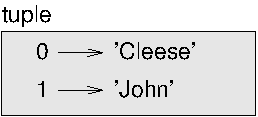
\includegraphics[scale=0.8]{figs/tuple1.pdf}}
\caption{State diagram.}
\label{fig.tuple1}
\end{figure}

But in a larger diagram you might want to leave out the
details.  For example, a diagram of the telephone directory might
appear as in Figure~\ref{fig.dict2}.

\begin{figure}
\centerline
{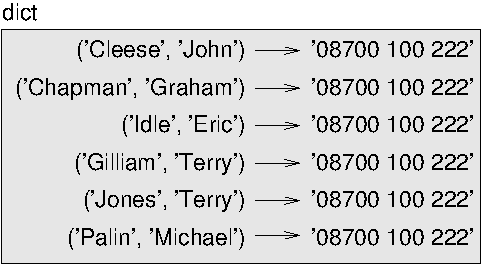
\includegraphics[scale=0.8]{figs/dict2.pdf}}
\caption{State diagram.}
\label{fig.dict2}
\end{figure}

Here the tuples are shown using Python syntax as a graphical
shorthand.

The telephone number in the diagram is the complaints line for the
BBC, so please don't call it.



\section{Comparing tuples}
\index{comparison!tuple}
\index{tuple!comparison}
\index{sort method}
\index{method!sort}

The relational operators work with tuples and other sequences;
Python starts by comparing the first element from each
sequence.  If they are equal, it goes on to the next elements,
and so on, until it finds elements that differ.  Subsequent
elements are not considered (even if they are really big).

\begin{verbatim}
>>> (0, 1, 2) < (0, 3, 4)
True
>>> (0, 1, 2000000) < (0, 3, 4)
True
\end{verbatim}
%
The {\tt sort} function works the same way.  It sorts
primarily by first element, but in the case of a tie, it sorts
by second element, and so on.

This feature lends itself to a pattern called {\bf DSU} for

\begin{description}

\item[Decorate] a sequence by building a list of tuples
with one or more sort keys preceding the elements from the sequence,

\item[Sort] the list of tuples, and

\item[Undecorate] by extracting the sorted elements of the sequence.

\end{description}

\label{DSU}
\index{DSU pattern}
\index{pattern!DSU}
\index{decorate-sort-undecorate pattern}
\index{pattern!decorate-sort-undecorate}

For example, suppose you have a list of words and you want to
sort them from longest to shortest:

\begin{verbatim}
def sort_by_length(words):
    t = []
    for word in words:
       t.append((len(word), word))

    t.sort(reverse=True)

    res = []
    for length, word in t:
        res.append(word)
    return res
\end{verbatim}
%
The first loop builds a list of tuples, where each
tuple is a word preceded by its length.

{\tt sort} compares the first element, length, first, and
only considers the second element to break ties.  The keyword argument
{\tt reverse=True} tells {\tt sort} to go in decreasing order.
\index{keyword argument}
\index{argument!keyword}
\index{traversal}

The second loop traverses the list of tuples and builds a list of
words in descending order of length.

\begin{exercise}

In this example, ties are broken by comparing words, so words
with the same length appear in reverse alphabetical order.  For other
applications you might want to break ties at random.  Modify
this example so that words with the same length appear in
random order.  Hint: see the {\tt random} function in the
{\tt random} module.
Solution: \url{http://thinkpython.com/code/unstable_sort.py}.

\index{random module}
\index{module!random}
\index{random function}
\index{function!random}

\end{exercise}


\section{Sequences of sequences}
\index{sequence}

I have focused on lists of tuples, but almost all of the examples in
this chapter also work with lists of lists, tuples of tuples, and
tuples of lists.  To avoid enumerating the possible combinations, it
is sometimes easier to talk about sequences of sequences.

In many contexts, the different kinds of sequences (strings, lists and
tuples) can be used interchangeably.  So how and why do you choose one
over the others?
\index{string}
\index{list}
\index{tuple}
\index{mutability}
\index{immutability}

To start with the obvious, strings are more limited than other
sequences because the elements have to be characters.  They are
also immutable.  If you need the ability to change the characters
in a string (as opposed to creating a new string), you might
want to use a list of characters instead.

Lists are more common than tuples, mostly because they are mutable.
But there are a few cases where you might prefer tuples:

\begin{enumerate}

\item In some contexts, like a {\tt return} statement, it is
syntactically simpler to create a tuple than a list.  In other
contexts, you might prefer a list.

\item If you want to use a sequence as a dictionary key, you
have to use an immutable type like a tuple or string.

\item If you are passing a sequence as an argument to a function,
using tuples reduces the potential for unexpected behavior
due to aliasing.

\end{enumerate}

Because tuples are immutable, they don't provide methods
like {\tt sort} and {\tt reverse}, which modify existing lists.
But Python provides the built-in functions {\tt sorted}
and {\tt reversed}, which take any sequence as a parameter
and return a new list with the same elements in a different
order.
\index{sorted function}
\index{function!sorted}
\index{reversed function}
\index{function!reversed}


\section{Debugging}
\index{debugging}
\index{data structure}
\index{shape error}
\index{error!shape}

Lists, dictionaries and tuples are known generically as {\bf data
  structures}; in this chapter we are starting to see compound data
structures, like lists of tuples, and dictionaries that contain tuples
as keys and lists as values.  Compound data structures are useful, but
they are prone to what I call {\bf shape errors}; that is, errors
caused when a data structure has the wrong type, size or composition.
For example, if you are expecting a list with one integer and I
give you a plain old integer (not in a list), it won't work.
\index{structshape module}
\index{module!structshape}

% TODO: structshape is now part of Swampy

To help debug these kinds of errors, I have written a module
called {\tt structshape} that provides a function, also called
{\tt structshape}, that takes any kind of data structure as
an argument and returns a string that summarizes its shape.
You can download it from \url{http://thinkpython.com/code/structshape.py}

Here's the result for a simple list:

\begin{verbatim}
>>> from structshape import structshape
>>> t = [1,2,3]
>>> print structshape(t)
list of 3 int
\end{verbatim}
%
A fancier program might write ``list of 3 int{\em s},'' but it
was easier not to deal with plurals.  Here's a list of lists:

\begin{verbatim}
>>> t2 = [[1,2], [3,4], [5,6]]
>>> print structshape(t2)
list of 3 list of 2 int
\end{verbatim}
%
If the elements of the list are not the same type,
{\tt structshape} groups them, in order, by type:

\begin{verbatim}
>>> t3 = [1, 2, 3, 4.0, '5', '6', [7], [8], 9]
>>> print structshape(t3)
list of (3 int, float, 2 str, 2 list of int, int)
\end{verbatim}
%
Here's a list of tuples:

\begin{verbatim}
>>> s = 'abc'
>>> lt = zip(t, s)
>>> print structshape(lt)
list of 3 tuple of (int, str)
\end{verbatim}
%
And here's a dictionary with 3 items that map integers to strings.

\begin{verbatim}
>>> d = dict(lt)
>>> print structshape(d)
dict of 3 int->str
\end{verbatim}
%
If you are having trouble keeping track of your data structures,
{\tt structshape} can help.


\section{Glossary}

\begin{description}

\item[tuple:] An immutable sequence of elements.
\index{tuple}

\item[tuple assignment:] An assignment with a sequence on the
right side and a tuple of variables on the left.  The right
side is evaluated and then its elements are assigned to the
variables on the left.
\index{tuple assignment}
\index{assignment!tuple}

\item[gather:] The operation of assembling a variable-length
argument tuple.
\index{gather}

\item[scatter:] The operation of treating a sequence as a list of
arguments.
\index{scatter}

\item[DSU:] Abbreviation of ``decorate-sort-undecorate,'' a
pattern that involves building a list of tuples, sorting, and
extracting part of the result.
\index{DSU pattern}

\item[data structure:] A collection of related values, often
organized in lists, dictionaries, tuples, etc.
\index{data structure}

\item[shape (of a data structure):] A summary of the type,
size and composition of a data structure.
\index{shape}

\end{description}


\section{Exercises}

\begin{exercise}

Write a function called \verb"most_frequent" that takes a string and
prints the letters in decreasing order of frequency.  Find text
samples from several different languages and see how letter frequency
varies between languages.  Compare your results with the tables at
\url{http://en.wikipedia.org/wiki/Letter_frequencies}.  Solution:
\url{http://thinkpython.com/code/most_frequent.py}.  \index{letter
  frequency} \index{frequency!letter}

\end{exercise}


\begin{exercise}
\label{anagrams}
\index{anagram set}
\index{set!anagram}

More anagrams!

\begin{enumerate}

\item Write a program
that reads a word list from a file (see Section~\ref{wordlist}) and
prints all the sets of words that are anagrams.

Here is an example of what the output might look like:

\begin{verbatim}
['deltas', 'desalt', 'lasted', 'salted', 'slated', 'staled']
['retainers', 'ternaries']
['generating', 'greatening']
['resmelts', 'smelters', 'termless']
\end{verbatim}
%
Hint: you might want to build a dictionary that maps from a
set of letters to a list of words that can be spelled with those
letters.  The question is, how can you represent the set of
letters in a way that can be used as a key?

\item Modify the previous program so that it prints the largest set
of anagrams first, followed by the second largest set, and so on.
\index{Scrabble}
\index{bingo}

\item In Scrabble a ``bingo'' is when you play all seven tiles in
your rack, along with a letter on the board, to form an eight-letter
word.  What set of 8 letters forms the most possible bingos?
Hint: there are seven.

% (7, ['angriest', 'astringe', 'ganister', 'gantries', 'granites',
% 'ingrates', 'rangiest'])

Solution: \url{http://thinkpython.com/code/anagram_sets.py}.

\end{enumerate}
\end{exercise}

\begin{exercise}
\index{metathesis}

Two words form a ``metathesis pair'' if you can transform one into the
other by swapping two letters; for example, ``converse'' and
``conserve.''  Write a program that finds all of the metathesis pairs
in the dictionary.  Hint: don't test all pairs of words, and don't
test all possible swaps.  Solution: \url{http://thinkpython.com/code/metathesis.py}.
Credit: This exercise is inspired by an example at \url{http://puzzlers.org}.

\end{exercise}



\begin{exercise}
\index{Car Talk}
\index{Puzzler}

Here's another Car Talk Puzzler
(\url{http://www.cartalk.com/content/puzzlers}):

\begin{quote}
What is the longest English word, that remains a valid English word,
as you remove its letters one at a time?

Now, letters can be removed from either end, or the middle, but you
can't rearrange any of the letters. Every time you drop a letter, you
wind up with another English word. If you do that, you're eventually
going to wind up with one letter and that too is going to be an
English word---one that's found in the dictionary. I want to know
what's the longest word and how many letters does it
have?

I'm going to give you a little modest example: Sprite. Ok? You start
off with sprite, you take a letter off, one from the interior of the
word, take the r away, and we're left with the word spite, then we
take the e off the end, we're left with spit, we take the s off, we're
left with pit, it, and I.
\end{quote}
\index{reducible word}
\index{word, reducible}

Write a program to find all words that can be reduced in this way,
and then find the longest one.

This exercise is a little more challenging than most, so here are
some suggestions:

\begin{enumerate}

\item You might want to write a function that takes a word and
  computes a list of all the words that can be formed by removing one
  letter.  These are the ``children'' of the word.
\index{recursive definition}
\index{definition!recursive}

\item Recursively, a word is reducible if any of its children
are reducible.  As a base case, you can consider the empty
string reducible.

\item The wordlist I provided, {\tt words.txt}, doesn't
contain single letter words.  So you might want to add
``I'', ``a'', and the empty string.

\item To improve the performance of your program, you might want
to memoize the words that are known to be reducible.

\end{enumerate}

Solution: \url{http://thinkpython.com/code/reducible.py}.

\end{exercise}




%\begin{exercise}
%\url{http://en.wikipedia.org/wiki/Word_Ladder}
%\end{exercise}




\chapter{Case study: data structure selection}

\section{Word frequency analysis}
\label{analysis}

As usual, you should at least attempt the following exercises
before you read my solutions.

\begin{exercise}

Write a program that reads a file, breaks each line into
words, strips whitespace and punctuation from the words, and
converts them to lowercase.
\index{string module}
\index{module!string}

Hint: The {\tt string} module provides strings named {\tt whitespace},
which contains space, tab, newline, etc., and {\tt
  punctuation} which contains the punctuation characters.  Let's see
if we can make Python swear:

\begin{verbatim}
>>> import string
>>> print string.punctuation
!"#$%&'()*+,-./:;<=>?@[\]^_`{|}~
\end{verbatim}
%
Also, you might consider using the string methods {\tt strip},
{\tt replace} and {\tt translate}.
\index{strip method}
\index{method!strip}
\index{replace method}
\index{method!replace}
\index{translate method}
\index{method!translate}

\end{exercise}


\begin{exercise}
\index{Project Gutenberg}

Go to Project Gutenberg (\url{gutenberg.org}) and download
your favorite out-of-copyright book in plain text format.
\index{plain text}
\index{text!plain}

Modify your program from the previous exercise to read the book
you downloaded, skip over the header information at the beginning
of the file, and process the rest of the words as before.

Then modify the program to count the total number of words in
the book, and the number of times each word is used.
\index{word frequency}
\index{frequency!word}

Print the number of different words used in the book.  Compare
different books by different authors, written in different eras.
Which author uses the most extensive vocabulary?
\end{exercise}


\begin{exercise}

Modify the program from the previous exercise to print the
20 most frequently-used words in the book.

\end{exercise}


\begin{exercise}

Modify the previous program to read a word list (see
Section~\ref{wordlist}) and then print all the words in the book that
are not in the word list.  How many of them are typos?  How many of
them are common words that {\em should} be in the word list, and how
many of them are really obscure?

\end{exercise}


\section{Random numbers}
\index{random number}
\index{number, random}
\index{deterministic}
\index{pseudorandom}

Given the same inputs, most computer programs generate the same
outputs every time, so they are said to be {\bf deterministic}.
Determinism is usually a good thing, since we expect the same
calculation to yield the same result.  For some applications, though,
we want the computer to be unpredictable.  Games are an obvious
example, but there are more.

Making a program truly nondeterministic turns out to be not so easy,
but there are ways to make it at least seem nondeterministic.  One of
them is to use algorithms that generate {\bf pseudorandom} numbers.
Pseudorandom numbers are not truly random because they are generated
by a deterministic computation, but just by looking at the numbers it
is all but impossible to distinguish them from random.
\index{random module}
\index{module!random}

The {\tt random} module provides functions that generate
pseudorandom numbers (which I will simply call ``random'' from
here on).
\index{random function}
\index{function!random}

The function {\tt random} returns a random float
between 0.0 and 1.0 (including 0.0 but not 1.0).  Each time you
call {\tt random}, you get the next number in a long series.  To see a
sample, run this loop:

\begin{verbatim}
import random

for i in range(10):
    x = random.random()
    print x
\end{verbatim}
%
The function {\tt randint} takes parameters {\tt low} and
{\tt high} and returns an integer between {\tt low} and
{\tt high} (including both).
\index{randint function}
\index{function!randint}

\begin{verbatim}
>>> random.randint(5, 10)
5
>>> random.randint(5, 10)
9
\end{verbatim}
%
To choose an element from a sequence at random, you can use
{\tt choice}:
\index{choice function}
\index{function!choice}

\begin{verbatim}
>>> t = [1, 2, 3]
>>> random.choice(t)
2
>>> random.choice(t)
3
\end{verbatim}
%
The {\tt random} module also provides functions to generate
random values from continuous distributions including
Gaussian, exponential, gamma, and a few more.

\begin{exercise}
\index{histogram!random choice}

Write a function named \verb"choose_from_hist" that takes
a histogram as defined in Section~\ref{histogram} and returns a
random value from the histogram, chosen with probability
in proportion to frequency.  For example, for this histogram:

\begin{verbatim}
>>> t = ['a', 'a', 'b']
>>> hist = histogram(t)
>>> print hist
{'a': 2, 'b': 1}
\end{verbatim}
%
your function should return {\tt 'a'} with probability $2/3$ and {\tt 'b'}
with probability $1/3$.
\end{exercise}


\section{Word histogram}

You should attempt the previous exercises before you go on.
You can download my solution from
 \url{http://thinkpython.com/code/analyze_book.py}.  You will
also need \url{http://thinkpython.com/code/emma.txt}.

Here is a program that reads a file and builds a histogram of the
words in the file:
\index{histogram!word frequencies}

\begin{verbatim}
import string

def process_file(filename):
    hist = dict()
    fp = open(filename)
    for line in fp:
        process_line(line, hist)
    return hist

def process_line(line, hist):
    line = line.replace('-', ' ')

    for word in line.split():
        word = word.strip(string.punctuation + string.whitespace)
        word = word.lower()

        hist[word] = hist.get(word, 0) + 1

hist = process_file('emma.txt')
\end{verbatim}
%
This program reads {\tt emma.txt}, which contains the text of {\em
  Emma} by Jane Austen.
\index{Austin, Jane}

\verb"process_file" loops through the lines of the file,
passing them one at a time to \verb"process_line".  The histogram
{\tt hist} is being used as an accumulator.
\index{accumulator!histogram}
\index{traversal}

\verb"process_line" uses the string method {\tt replace} to replace
hyphens with spaces before using {\tt split} to break the line into a
list of strings.  It traverses the list of words and uses {\tt strip}
and {\tt lower} to remove punctuation and convert to lower case.  (It
is a shorthand to say that strings are ``converted;'' remember that
string are immutable, so methods like {\tt strip} and {\tt lower}
return new strings.)

Finally, \verb"process_line" updates the histogram by creating a new
item or incrementing an existing one.
\index{update!histogram}

To count the total number of words in the file, we can add up
the frequencies in the histogram:

\begin{verbatim}
def total_words(hist):
    return sum(hist.values())
\end{verbatim}
%
The number of different words is just the number of items in
the dictionary:

\begin{verbatim}
def different_words(hist):
    return len(hist)
\end{verbatim}
%
Here is some code to print the results:

\begin{verbatim}
print 'Total number of words:', total_words(hist)
print 'Number of different words:', different_words(hist)
\end{verbatim}
%
And the results:

\begin{verbatim}
Total number of words: 161080
Number of different words: 7214
\end{verbatim}
%

\section{Most common words}
\index{DSU pattern}
\index{pattern!DSU}

To find the most common words, we can apply the DSU pattern;
\verb"most_common" takes a histogram and returns a list of
word-frequency tuples, sorted in reverse order by frequency:

\begin{verbatim}
def most_common(hist):
    t = []
    for key, value in hist.items():
        t.append((value, key))

    t.sort(reverse=True)
    return t
\end{verbatim}
%
Here is a loop that prints the ten most common words:

\begin{verbatim}
t = most_common(hist)
print 'The most common words are:'
for freq, word in t[0:10]:
    print word, '\t', freq
\end{verbatim}
%
And here are the results from {\em Emma}:

\begin{verbatim}
The most common words are:
to 	5242
the 	5205
and 	4897
of 	4295
i 	3191
a 	3130
it 	2529
her 	2483
was 	2400
she 	2364
\end{verbatim}
%

\section{Optional parameters}
\index{optional parameter}
\index{parameter!optional}

We have seen built-in functions and methods that take a variable
number of arguments.  It is possible to write user-defined functions
with optional arguments, too.  For example, here is a function that
prints the most common words in a histogram

\begin{verbatim}
def print_most_common(hist, num=10):
    t = most_common(hist)
    print 'The most common words are:'
    for freq, word in t[:num]:
        print word, '\t', freq
\end{verbatim}

The first parameter is required; the second is optional.
The {\bf default value} of {\tt num} is 10.
\index{default value}
\index{value!default}

If you only provide one argument:

\begin{verbatim}
print_most_common(hist)
\end{verbatim}

{\tt num} gets the default value.  If you provide two arguments:

\begin{verbatim}
print_most_common(hist, 20)
\end{verbatim}

{\tt num} gets the value of the argument instead.  In other
words, the optional argument {\bf overrides} the default value.
\index{override}

If a function has both required and optional parameters, all
the required parameters have to come first, followed by the
optional ones.


\section{Dictionary subtraction}
\index{dictionary!subtraction}
\index{subtraction!dictionary}

Finding the words from the book that are not in the word list
from {\tt words.txt} is a problem you might recognize as set
subtraction; that is, we want to find all the words from one
set (the words in the book) that are not in another set (the
words in the list).

{\tt subtract} takes dictionaries {\tt d1} and {\tt d2} and returns a
new dictionary that contains all the keys from {\tt d1} that are not
in {\tt d2}.  Since we don't really care about the values, we
set them all to None.

\begin{verbatim}
def subtract(d1, d2):
    res = dict()
    for key in d1:
        if key not in d2:
            res[key] = None
    return res
\end{verbatim}
%
To find the words in the book that are not in {\tt words.txt},
we can use \verb"process_file" to build a histogram for
{\tt words.txt}, and then subtract:

\begin{verbatim}
words = process_file('words.txt')
diff = subtract(hist, words)

print "The words in the book that aren't in the word list are:"
for word in diff.keys():
    print word,
\end{verbatim}
%
Here are some of the results from {\em Emma}:

\begin{verbatim}
The words in the book that aren't in the word list are:
 rencontre jane's blanche woodhouses disingenuousness
friend's venice apartment ...
\end{verbatim}
%
Some of these words are names and possessives.  Others, like
``rencontre,'' are no longer in common use.  But a few are common
words that should really be in the list!

\begin{exercise}
\index{set}
\index{type!set}

Python provides a data structure called {\tt set} that provides many
common set operations.  Read the documentation at
\url{http://docs.python.org/2/library/stdtypes.html#types-set} and
write a program that uses set subtraction to find words in the book
that are not in the word list.  Solution:
\url{http://thinkpython.com/code/analyze_book2.py}.

\end{exercise}


\section{Random words}
\label{randomwords}
\index{histogram!random choice}

To choose a random word from the histogram, the simplest algorithm
is to build a list with multiple copies of each word, according
to the observed frequency, and then choose from the list:

\begin{verbatim}
def random_word(h):
    t = []
    for word, freq in h.items():
        t.extend([word] * freq)

    return random.choice(t)
\end{verbatim}
%
The expression {\tt [word] * freq} creates a list with {\tt freq}
copies of the string {\tt word}.  The {\tt extend}
method is similar to {\tt append} except that the argument is
a sequence.

\begin{exercise}
\label{randhist}
\index{algorithm}

This algorithm works, but it is not very efficient; each time you
choose a random word, it rebuilds the list, which is as big as
the original book.  An obvious improvement is to build the list
once and then make multiple selections, but the list is still big.

An alternative is:

\begin{enumerate}

\item Use {\tt keys} to get a list of the words in the book.

\item Build a list that contains the cumulative sum of the word
  frequencies (see Exercise~\ref{cumulative}).  The last item
  in this list is the total number of words in the book, $n$.

\item Choose a random number from 1 to $n$.  Use a bisection search
  (See Exercise~\ref{bisection}) to find the index where the random
  number would be inserted in the cumulative sum.

\item Use the index to find the corresponding word in the word list.

\end{enumerate}

Write a program that uses this algorithm to choose a random
word from the book.  Solution: \url{http://thinkpython.com/code/analyze_book3.py}.

\end{exercise}



\section{Markov analysis}
\label{markov}
\index{Markov analysis}

If you choose words from the book at random, you can get a
sense of the vocabulary, you probably won't get a sentence:

\begin{verbatim}
this the small regard harriet which knightley's it most things
\end{verbatim}
%
A series of random words seldom makes sense because there
is no relationship between successive words.  For example, in
a real sentence you would expect an article like ``the'' to
be followed by an adjective or a noun, and probably not a verb
or adverb.

One way to measure these kinds of relationships is Markov
analysis, which
characterizes, for a given sequence of words, the probability of the
word that comes next.  For example, the song {\em Eric, the Half a
  Bee} begins:

\begin{quote}
Half a bee, philosophically, \\
Must, ipso facto, half not be. \\
But half the bee has got to be \\
Vis a vis, its entity. D'you see? \\
\\
But can a bee be said to be \\
Or not to be an entire bee \\
When half the bee is not a bee \\
Due to some ancient injury? \\
\end{quote}
%
In this text,
the phrase ``half the'' is always followed by the word ``bee,''
but the phrase ``the bee'' might be followed by either
``has'' or ``is''.
\index{prefix}
\index{suffix}
\index{mapping}

The result of Markov analysis is a mapping from each prefix
(like ``half the'' and ``the bee'') to all possible suffixes
(like ``has'' and ``is'').
\index{random text}
\index{text!random}

Given this mapping, you can generate a random text by
starting with any prefix and choosing at random from the
possible suffixes.  Next, you can combine the end of the
prefix and the new suffix to form the next prefix, and repeat.

For example, if you start with the prefix ``Half a,'' then the
next word has to be ``bee,'' because the prefix only appears
once in the text.  The next prefix is ``a bee,'' so the
next suffix might be ``philosophically,'' ``be'' or ``due.''

In this example the length of the prefix is always two, but
you can do Markov analysis with any prefix length.  The length
of the prefix is called the ``order'' of the analysis.

\begin{exercise}

Markov analysis:

\begin{enumerate}

\item Write a program to read a text from a file and perform Markov
analysis.  The result should be a dictionary that maps from
prefixes to a collection of possible suffixes.  The collection
might be a list, tuple, or dictionary; it is up to you to make
an appropriate choice.  You can test your program with prefix
length two, but you should write the program in a way that makes
it easy to try other lengths.

\item Add a function to the previous program to generate random text
based on the Markov analysis.  Here is an example from {\em Emma}
with prefix length 2:

\begin{quote}
He was very clever, be it sweetness or be angry, ashamed or only
amused, at such a stroke. She had never thought of Hannah till you
were never meant for me?" "I cannot make speeches, Emma:" he soon cut
it all himself.
\end{quote}

For this example, I left the punctuation attached to the words.
The result is almost syntactically correct, but not quite.
Semantically, it almost makes sense, but not quite.

What happens if you increase the prefix length?  Does the random
text make more sense?
\index{mash-up}

\item Once your program is working, you might want to try a mash-up:
if you analyze text from two or more books, the random
text you generate will blend the vocabulary and phrases from
the sources in interesting ways.

\end{enumerate}

Credit: This case study is based on an example from Kernighan and
Pike, {\em The Practice of Programming}, Addison-Wesley, 1999.

\end{exercise}

You should attempt this exercise before you go on; then you can can
download my solution from \url{http://thinkpython.com/code/markov.py}.  You
will also need \url{http://thinkpython.com/code/emma.txt}.


\section{Data structures}
\index{data structure}

Using Markov analysis to generate random text is fun, but there is
also a point to this exercise: data structure selection.  In your
solution to the previous exercises, you had to choose:

\begin{itemize}

\item How to represent the prefixes.

\item How to represent the collection of possible suffixes.

\item How to represent the mapping from each prefix to
the collection of possible suffixes.

\end{itemize}

Ok, the last one is the easy; the only mapping type we have
seen is a dictionary, so it is the natural choice.

For the prefixes, the most obvious options are string,
list of strings, or tuple of strings.  For the suffixes,
one option is a list; another is a histogram (dictionary).
\index{implementation}

How should you choose?  The first step is to think about
the operations you will need to implement for each data structure.
For the prefixes, we need to be able to remove words from
the beginning and add to the end.  For example, if the current
prefix is ``Half a,'' and the next word is ``bee,'' you need
to be able to form the next prefix, ``a bee.''
\index{tuple!as key in dictionary}

Your first choice might be a list, since it is easy to add
and remove elements, but we also need to be able to use the
prefixes as keys in a dictionary, so that rules out lists.
With tuples, you can't append or remove, but you can use
the addition operator to form a new tuple:

\begin{verbatim}
def shift(prefix, word):
    return prefix[1:] + (word,)
\end{verbatim}
%
{\tt shift} takes a tuple of words, {\tt prefix}, and a string,
{\tt word}, and forms a new tuple that has all the words
in {\tt prefix} except the first, and {\tt word} added to
the end.

For the collection of suffixes, the operations we need to
perform include adding a new suffix (or increasing the frequency
of an existing one), and choosing a random suffix.

Adding a new suffix is equally easy for the list implementation
or the histogram.  Choosing a random element from a list
is easy; choosing from a histogram is harder to do
efficiently (see Exercise~\ref{randhist}).

So far we have been talking mostly about ease of implementation,
but there are other factors to consider in choosing data structures.
One is run time.  Sometimes there is a theoretical reason to expect
one data structure to be faster than other; for example, I mentioned
that the {\tt in} operator is faster for dictionaries than for lists,
at least when the number of elements is large.

But often you don't know ahead of time which implementation will
be faster.  One option is to implement both of them and see which
is better.  This approach is called {\bf benchmarking}.  A practical
alternative is to choose the data structure that is
easiest to implement, and then see if it is fast enough for the
intended application.  If so, there is no need to go on.  If not,
there are tools, like the {\tt profile} module, that can identify
the places in a program that take the most time.
\index{benchmarking}
\index{profile module}
\index{module!profile}

The other factor to consider is storage space.  For example, using a
histogram for the collection of suffixes might take less space because
you only have to store each word once, no matter how many times it
appears in the text.  In some cases, saving space can also make your
program run faster, and in the extreme, your program might not run at
all if you run out of memory.  But for many applications, space is a
secondary consideration after run time.

One final thought: in this discussion, I have implied that
we should use one data structure for both analysis and generation.  But
since these are separate phases, it would also be possible to use one
structure for analysis and then convert to another structure for
generation.  This would be a net win if the time saved during
generation exceeded the time spent in conversion.


\section{Debugging}
\index{debugging}

When you are debugging a program, and especially if you are
working on a hard bug, there are four things to try:

\begin{description}

\item[reading:] Examine your code, read it back to yourself, and
check that it says what you meant to say.

\item[running:] Experiment by making changes and running different
versions.  Often if you display the right thing at the right place
in the program, the problem becomes obvious, but sometimes you have to
spend some time to build scaffolding.

\item[ruminating:] Take some time to think!  What kind of error
is it: syntax, runtime, semantic?  What information can you get from
the error messages, or from the output of the program?  What kind of
error could cause the problem you're seeing?  What did you change
last, before the problem appeared?

\item[retreating:] At some point, the best thing to do is back
off, undoing recent changes, until you get back to a program that
works and that you understand.  Then you can start rebuilding.

\end{description}

Beginning programmers sometimes get stuck on one of these activities
and forget the others.  Each activity comes with its own failure
mode.
\index{typographical error}

For example, reading your code might help if the problem is a
typographical error, but not if the problem is a conceptual
misunderstanding.  If you don't understand what your program does, you
can read it 100 times and never see the error, because the error is in
your head.
\index{experimental debugging}

Running experiments can help, especially if you run small, simple
tests.  But if you run experiments without thinking or reading your
code, you might fall into a pattern I call ``random walk programming,''
which is the process of making random changes until the program
does the right thing.  Needless to say, random walk programming
can take a long time.
\index{random walk programming}
\index{development plan!random walk programming}

You have to take time to think.  Debugging is like an
experimental science.  You should have at least one hypothesis about
what the problem is.  If there are two or more possibilities, try to
think of a test that would eliminate one of them.

Taking a break helps with the thinking.  So does talking.
If you explain the problem to someone else (or even yourself), you
will sometimes find the answer before you finish asking the question.

But even the best debugging techniques will fail if there are too many
errors, or if the code you are trying to fix is too big and
complicated.  Sometimes the best option is to retreat, simplifying the
program until you get to something that works and that you
understand.

Beginning programmers are often reluctant to retreat because
they can't stand to delete a line of code (even if it's wrong).
If it makes you feel better, copy your program into another file
before you start stripping it down.  Then you can paste the pieces
back in a little bit at a time.

Finding a hard bug requires reading, running, ruminating, and
sometimes retreating.  If you get stuck on one of these activities,
try the others.


\section{Glossary}

\begin{description}

\item[deterministic:] Pertaining to a program that does the same
thing each time it runs, given the same inputs.
\index{deterministic}

\item[pseudorandom:] Pertaining to a sequence of numbers that appear
to be random, but are generated by a deterministic program.
\index{pseudorandom}

\item[default value:] The value given to an optional parameter if no
argument is provided.
\index{default value}

\item[override:] To replace a default value with an argument.
\index{override}

\item[benchmarking:] The process of choosing between data structures
by implementing alternatives and testing them on a sample of the
possible inputs.
\index{benchmarking}

\end{description}


\section{Exercises}

\begin{exercise}
\index{word frequency}
\index{frequency!word}
\index{Zipf's law}

The ``rank'' of a word is its position in a list of words
sorted by frequency: the most common word has rank 1, the
second most common has rank 2, etc.

Zipf's law describes a relationship between the ranks and frequencies
of words in natural languages
(\url{http://en.wikipedia.org/wiki/Zipf's_law}).  Specifically, it
predicts that the frequency, $f$, of the word with rank $r$ is:

\[ f = c r^{-s} \]
%
where $s$ and $c$ are parameters that depend on the language and the
text.  If you take the logarithm of both sides of this equation, you
get:
\index{logarithm}

\[ \log f = \log c - s \log r \]
%
So if you plot log $f$ versus log $r$, you should get
a straight line with slope $-s$ and intercept log $c$.

Write a program that reads a text from a file, counts
word frequencies, and prints one line
for each word, in descending order of frequency, with
log $f$ and log $r$.  Use the graphing program of your
choice to plot the results and check whether they form
a straight line.  Can you estimate the value of $s$?

Solution: \url{http://thinkpython.com/code/zipf.py}.  To make the plots, you
might have to install matplotlib (see
\url{http://matplotlib.sourceforge.net/}).
\index{Matplotlib}

\end{exercise}


\chapter{Files}


\section{Persistence}
\index{file}
\index{type!file}
\index{persistence}

Most of the programs we have seen so far are transient in the
sense that they run for a short time and produce some output,
but when they end, their data disappears.  If you run the program
again, it starts with a clean slate.

Other programs are {\bf persistent}: they run for a long time
(or all the time); they keep at least some of their data
in permanent storage (a hard drive, for example); and
if they shut down and restart, they pick up where they left off.

Examples of persistent programs are operating systems, which
run pretty much whenever a computer is on, and web servers,
which run all the time, waiting for requests to come in on
the network.

One of the simplest ways for programs to maintain their data
is by reading and writing text files.  We have already seen
programs that read text files; in this chapter we will see programs
that write them.

An alternative is to store the state of the program in a database.
In this chapter I will present a simple database and a module,
{\tt pickle}, that makes it easy to store program data.
\index{pickle module}
\index{module!pickle}


\section{Reading and writing}
\index{file!reading and writing}

A text file is a sequence of characters stored on a permanent
medium like a hard drive, flash memory, or CD-ROM.  We saw how
to open and read a file in Section~\ref{wordlist}.
\index{open function}
\index{function!open}

To write a file, you have to open it with mode \verb"'w'" as a second
parameter:

\begin{verbatim}
>>> fout = open('output.txt', 'w')
>>> print fout
<open file 'output.txt', mode 'w' at 0xb7eb2410>
\end{verbatim}
%
If the file already exists, opening it in write mode clears out
the old data and starts fresh, so be careful!
If the file doesn't exist, a new one is created.

The {\tt write} method puts data into the file.

\begin{verbatim}
>>> line1 = "This here's the wattle,\n"
>>> fout.write(line1)
\end{verbatim}
%
Again, the file object keeps track of where it is, so if
you call {\tt write} again, it adds the new data to the end.

\begin{verbatim}
>>> line2 = "the emblem of our land.\n"
>>> fout.write(line2)
\end{verbatim}
%
When you are done writing, you have to close the file.

\begin{verbatim}
>>> fout.close()
\end{verbatim}
%
\index{close method}
\index{method!close}


\section{Format operator}
\index{format operator}
\index{operator!format}

The argument of {\tt write} has to be a string, so if we want
to put other values in a file, we have to convert them to
strings.  The easiest way to do that is with {\tt str}:

\begin{verbatim}
>>> x = 52
>>> f.write(str(x))
\end{verbatim}
%
An alternative is to use the {\bf format operator}, {\tt \%}.  When
applied to integers, {\tt \%} is the modulus operator.  But
when the first operand is a string, {\tt \%} is the format operator.
\index{format string}

The first operand is the {\bf format string}, which contains
one or more {\bf format sequences}, which
specify how
the second operand is formatted.  The result is a string.
\index{format sequence}

For example, the format sequence \verb"'%d'" means that
the second operand should be formatted as an
integer ({\tt d} stands for ``decimal''):

\begin{verbatim}
>>> camels = 42
>>> '%d' % camels
'42'
\end{verbatim}
%
The result is the string \verb"'42'", which is not to be confused
with the integer value {\tt 42}.

A format sequence can appear anywhere in the string,
so you can embed a value in a sentence:

\begin{verbatim}
>>> camels = 42
>>> 'I have spotted %d camels.' % camels
'I have spotted 42 camels.'
\end{verbatim}
%
If there is more than one format sequence in the string,
the second argument has to be a tuple.  Each format sequence is
matched with an element of the tuple, in order.

The following example uses \verb"'%d'" to format an integer,
\verb"'%g'" to format
a floating-point number (don't ask why), and \verb"'%s'" to format
a string:

\begin{verbatim}
>>> 'In %d years I have spotted %g %s.' % (3, 0.1, 'camels')
'In 3 years I have spotted 0.1 camels.'
\end{verbatim}
%
The number of elements in the tuple has to match the number
of format sequences in the string.  Also, the types of the
elements have to match the format sequences:
\index{exception!TypeError}
\index{TypeError}

\begin{verbatim}
>>> '%d %d %d' % (1, 2)
TypeError: not enough arguments for format string
>>> '%d' % 'dollars'
TypeError: illegal argument type for built-in operation
\end{verbatim}
%
In the first example, there aren't enough elements; in the
second, the element is the wrong type.

The format operator is powerful, but it can be difficult to use.  You
can read more about it at
\url{http://docs.python.org/2/library/stdtypes.html#string-formatting}.

% You can specify the number of digits as part of the format sequence.
% For example, the sequence \verb"'%8.2f'"
% formats a floating-point number to be 8 characters long, with
% 2 digits after the decimal point:

% % \begin{verbatim}
% >>> '%8.2f' % 3.14159
% '    3.14'
% \end{verbatim}
% \afterverb
% %
% The result takes up eight spaces with two
% digits after the decimal point.


\section{Filenames and paths}
\label{paths}
\index{filename}
\index{path}
\index{directory}
\index{folder}

Files are organized into {\bf directories} (also called ``folders'').
Every running program has a ``current directory,'' which is the
default directory for most operations.
For example, when you open a file for reading, Python looks for it in the
current directory.
\index{os module}
\index{module!os}

The {\tt os} module provides functions for working with files and
directories (``os'' stands for ``operating system'').  {\tt os.getcwd}
returns the name of the current directory:
\index{getcwd function}
\index{function!getcwd}

\begin{verbatim}
>>> import os
>>> cwd = os.getcwd()
>>> print cwd
/home/dinsdale
\end{verbatim}
%
{\tt cwd} stands for ``current working directory.''  The result in
this example is {\tt /home/dinsdale}, which is the home directory of a
user named {\tt dinsdale}.
\index{working directory}
\index{directory!working}

A string like {\tt cwd} that identifies a file is called a {\bf path}.
A {\bf relative path} starts from the current directory;
an {\bf absolute path} starts from the topmost directory in the
file system.
\index{relative path}
\index{path!relative}
\index{absolute path}
\index{path!absolute}

The paths we have seen so far are simple filenames, so they are
relative to the current directory.  To find the absolute path to
a file, you can use {\tt os.path.abspath}:

\begin{verbatim}
>>> os.path.abspath('memo.txt')
'/home/dinsdale/memo.txt'
\end{verbatim}
%
{\tt os.path.exists} checks
whether a file or directory exists:
\index{exists function}
\index{function!exists}

\begin{verbatim}
>>> os.path.exists('memo.txt')
True
\end{verbatim}
%
If it exists, {\tt os.path.isdir} checks whether it's a directory:

\begin{verbatim}
>>> os.path.isdir('memo.txt')
False
>>> os.path.isdir('music')
True
\end{verbatim}
%
Similarly, {\tt os.path.isfile} checks whether it's a file.

{\tt os.listdir} returns a list of the files (and other directories)
in the given directory:

\begin{verbatim}
>>> os.listdir(cwd)
['music', 'photos', 'memo.txt']
\end{verbatim}
%
To demonstrate these functions, the following example
``walks'' through a directory, prints
the names of all the files, and calls itself recursively on
all the directories.
\index{walk, directory}
\index{directory!walk}

\begin{verbatim}
def walk(dirname):
    for name in os.listdir(dirname):
        path = os.path.join(dirname, name)

        if os.path.isfile(path):
            print path
        else:
            walk(path)
\end{verbatim}
%
{\tt os.path.join} takes a directory and a file name and joins
them into a complete path.

\begin{exercise}

The {\tt os} module provides a function called {\tt walk}
that is similar to this one but more versatile.  Read
the documentation and use it to print the names of the
files in a given directory and its subdirectories.

Solution: \url{http://thinkpython.com/code/walk.py}.

\end{exercise}


\section{Catching exceptions}
\label{catch}

A lot of things can go wrong when you try to read and write
files.  If you try to open a file that doesn't exist, you get an
{\tt IOError}:
\index{open function}
\index{function!open}
\index{exception!IOError}
\index{IOError}

\begin{verbatim}
>>> fin = open('bad_file')
IOError: [Errno 2] No such file or directory: 'bad_file'
\end{verbatim}
%
If you don't have permission to access a file:
\index{file!permission}
\index{permission, file}

\begin{verbatim}
>>> fout = open('/etc/passwd', 'w')
IOError: [Errno 13] Permission denied: '/etc/passwd'
\end{verbatim}
%
And if you try to open a directory for reading, you get

\begin{verbatim}
>>> fin = open('/home')
IOError: [Errno 21] Is a directory
\end{verbatim}
%
To avoid these errors, you could use functions like {\tt os.path.exists}
and {\tt os.path.isfile}, but it would take a lot of time and code
to check all the possibilities (if ``{\tt Errno 21}'' is any
indication, there are at least 21 things that can go wrong).
\index{exception, catching}
\index{try statement}
\index{statement!try}

It is better to go ahead and try---and deal with problems if they
happen---which is exactly what the {\tt try} statement does.  The
syntax is similar to an {\tt if} statement:

\begin{verbatim}
try:
    fin = open('bad_file')
    for line in fin:
        print line
    fin.close()
except:
    print 'Something went wrong.'
\end{verbatim}
%
Python starts by executing the {\tt try} clause.  If all goes
well, it skips the {\tt except} clause and proceeds.  If an
exception occurs, it jumps out of the {\tt try} clause and
executes the {\tt except} clause.

Handling an exception with a {\tt try} statement is called {\bf
catching} an exception.  In this example, the {\tt except} clause
prints an error message that is not very helpful.  In general,
catching an exception gives you a chance to fix the problem, or try
again, or at least end the program gracefully.

\begin{exercise}

Write a function called {\tt sed} that takes as arguments a pattern string,
a replacement string, and two filenames; it should read the first file
and write the contents into the second file (creating it if
necessary).  If the pattern string appears anywhere in the file, it
should be replaced with the replacement string.

If an error occurs while opening, reading, writing or closing files,
your program should catch the exception, print an error message, and
exit.  Solution: \url{http://thinkpython.com/code/sed.py}.

\end{exercise}


\section{Databases}
\index{database}

A {\bf database} is a file that is organized for storing data.
Most databases are organized like a dictionary in the sense
that they map from keys to values.  The biggest difference
is that the database is on disk (or other permanent storage),
so it persists after the program ends.
\index{anydbm module}
\index{module!anydbm}

The module {\tt anydbm} provides an interface for creating
and updating database files.  As an example, I'll create a database
that contains captions for image files.
\index{open function}
\index{function!open}

Opening a database is similar to opening other files:

\begin{verbatim}
>>> import anydbm
>>> db = anydbm.open('captions.db', 'c')
\end{verbatim}
%
The mode \verb"'c'" means that the database should be created if
it doesn't already exist.  The result is a database object
that can be used (for most operations) like a dictionary.
If you create a new item, {\tt anydbm} updates the database file.
\index{update!database}


\begin{verbatim}
>>> db['cleese.png'] = 'Photo of John Cleese.'
\end{verbatim}
%
When you access one of the items, {\tt anydbm} reads the file:

\begin{verbatim}
>>> print db['cleese.png']
Photo of John Cleese.
\end{verbatim}
%
If you make another assignment to an existing key, {\tt anydbm} replaces
the old value:

\begin{verbatim}
>>> db['cleese.png'] = 'Photo of John Cleese doing a silly walk.'
>>> print db['cleese.png']
Photo of John Cleese doing a silly walk.
\end{verbatim}
%
Many dictionary methods, like {\tt keys} and {\tt items}, also
work with database objects.  So does iteration with a {\tt for}
statement.
\index{dictionary methods!anydbm module}

\begin{verbatim}
for key in db:
    print key
\end{verbatim}
%
As with other files, you should close the database when you are
done:

\begin{verbatim}
>>> db.close()
\end{verbatim}
%
\index{close method}
\index{method!close}


\section{Pickling}
\index{pickling}

A limitation of {\tt anydbm} is that the keys and values have
to be strings.  If you try to use any other type, you get an
error.
\index{pickle module}
\index{module!pickle}

The {\tt pickle} module can help.  It translates
almost any type of object into a string suitable for storage in a
database, and then translates strings back into objects.

{\tt pickle.dumps} takes an object as a parameter and returns
a string representation ({\tt dumps} is short for ``dump string''):

\begin{verbatim}
>>> import pickle
>>> t = [1, 2, 3]
>>> pickle.dumps(t)
'(lp0\nI1\naI2\naI3\na.'
\end{verbatim}
%
The format isn't obvious to human readers; it is meant to be
easy for {\tt pickle} to interpret.  {\tt pickle.loads}
(``load string'') reconstitutes the object:

\begin{verbatim}
>>> t1 = [1, 2, 3]
>>> s = pickle.dumps(t1)
>>> t2 = pickle.loads(s)
>>> print t2
[1, 2, 3]
\end{verbatim}
%
Although the new object has the same value as the old, it is
not (in general) the same object:

\begin{verbatim}
>>> t1 == t2
True
>>> t1 is t2
False
\end{verbatim}
%
In other words, pickling and then unpickling has the same effect
as copying the object.

You can use {\tt pickle} to store non-strings in a database.
In fact, this combination is so common that it has been
encapsulated in a module called {\tt shelve}.
\index{shelve module}
\index{module!shelve}


\begin{exercise}
\index{anagram set}
\index{set!anagram}

If you download my solution to Exercise~\ref{anagrams} from
\url{http://thinkpython.com/code/anagram_sets.py}, you'll see that it creates
a dictionary that maps from a sorted string of letters to the list of
words that can be spelled with those letters.  For example, {\tt
  'opst'} maps to the list {\tt ['opts', 'post', 'pots', 'spot',
    'stop', 'tops']}.

Write a module that imports \verb"anagram_sets" and provides
two new functions: \verb"store_anagrams" should store the
anagram dictionary in a ``shelf;'' \verb"read_anagrams" should
look up a word and return a list of its anagrams.
Solution: \url{http://thinkpython.com/code/anagram_db.py}

\end{exercise}


\section{Pipes}
\index{shell}
\index{pipe}

Most operating systems provide a command-line interface,
also known as a {\bf shell}.  Shells usually provide commands
to navigate the file system and launch applications.  For
example, in Unix you can change directories with {\tt cd},
display the contents of a directory with {\tt ls}, and launch
a web browser by typing (for example) {\tt firefox}.
\index{ls (Unix command)}
\index{Unix command!ls}

Any program that you can launch from the shell can also be
launched from Python using a {\bf pipe}.  A pipe is an object
that represents a running program.

For example, the Unix command {\tt ls -l} normally displays the
contents of the current directory (in long format).  You can
launch {\tt ls} with {\tt os.popen}\footnote{{\tt popen} is deprecated
now, which means we are supposed to stop using it and start using
the {\tt subprocess} module.  But for simple cases, I find
{\tt subprocess} more complicated than necessary.  So I am going
to keep using {\tt popen} until they take it away.}:
\index{popen function}
\index{function!popen}

\begin{verbatim}
>>> cmd = 'ls -l'
>>> fp = os.popen(cmd)
\end{verbatim}
%
The argument is a string that contains a shell command.  The
return value is an object that behaves just like an open
file.  You can read the output from the {\tt ls} process one
line at a time with {\tt readline} or get the whole thing at
once with {\tt read}:
\index{readline method}
\index{method!readline}
\index{read method}
\index{method!read}

\begin{verbatim}
>>> res = fp.read()
\end{verbatim}
%
When you are done, you close the pipe like a file:
\index{close method}
\index{method!close}

\begin{verbatim}
>>> stat = fp.close()
>>> print stat
None
\end{verbatim}
%
The return value is the final status of the {\tt ls} process;
{\tt None} means that it ended normally (with no errors).

For example, most Unix systems provide a command called {\tt md5sum}
that reads the contents of a file and computes a ``checksum.''
You can read about MD5 at \url{http://en.wikipedia.org/wiki/Md5}.  This
command provides an efficient way to check whether two files
have the same contents.  The probability that different contents
yield the same checksum is very small (that is, unlikely to happen
before the universe collapses).
\index{md5}
\index{checksum}

You can use a pipe to run {\tt md5sum} from Python and get the result:

\begin{verbatim}
>>> filename = 'book.tex'
>>> cmd = 'md5sum ' + filename
>>> fp = os.popen(cmd)
>>> res = fp.read()
>>> stat = fp.close()
>>> print res
1e0033f0ed0656636de0d75144ba32e0  book.tex
>>> print stat
None
\end{verbatim}


\begin{exercise}
\label{checksum}
\index{MP3}

In a large collection of MP3 files, there may be more than one
copy of the same song, stored in different directories or with
different file names.  The goal of this exercise is to search for
duplicates.

\begin{enumerate}

\item Write a program that searches a directory and all of its
subdirectories, recursively, and returns a list of complete paths
for all files with a given suffix (like {\tt .mp3}).
Hint: {\tt os.path} provides several useful functions for
manipulating file and path names.
\index{duplicate}
\index{MD5 algorithm}
\index{algorithm!MD5}
\index{checksum}

\item To recognize duplicates, you can use {\tt md5sum}
to compute a ``checksum'' for each files.  If two files have
the same checksum, they probably have the same contents.
\index{md5sum}

\item To double-check, you can use the Unix command {\tt diff}.
\index{diff}

\end{enumerate}

Solution: \url{http://thinkpython.com/code/find_duplicates.py}.

\end{exercise}


\section{Writing modules}
\label{modules}
\index{module, writing}
\index{word count}

Any file that contains Python code can be imported as a module.
For example, suppose you have a file named {\tt wc.py} with the following
code:

\begin{verbatim}
def linecount(filename):
    count = 0
    for line in open(filename):
        count += 1
    return count

print linecount('wc.py')
\end{verbatim}
%
If you run this program, it reads itself and prints the number
of lines in the file, which is 7.
You can also import it like this:

\begin{verbatim}
>>> import wc
7
\end{verbatim}
%
Now you have a module object {\tt wc}:
\index{module object}
\index{object!module}

\begin{verbatim}
>>> print wc
<module 'wc' from 'wc.py'>
\end{verbatim}
%
That provides a function called \verb"linecount":

\begin{verbatim}
>>> wc.linecount('wc.py')
7
\end{verbatim}
%
So that's how you write modules in Python.

The only problem with this example is that when you import
the module it executes the test code at the bottom.  Normally
when you import a module, it defines new functions but it
doesn't execute them.
\index{import statement}
\index{statement!import}

Programs that will be imported as modules often
use the following idiom:

\begin{verbatim}
if __name__ == '__main__':
    print linecount('wc.py')
\end{verbatim}
%
\verb"__name__" is a built-in variable that is set when the
program starts.  If the program is running as a script,
\verb"__name__" has the value \verb"__main__"; in that
case, the test code is executed.  Otherwise,
if the module is being imported, the test code is skipped.

\begin{exercise}

Type this example into a file named {\tt wc.py} and run
it as a script.  Then run the Python interpreter and
{\tt import wc}.  What is the value of \verb"__name__"
when the module is being imported?

Warning: If you import a module that has already been imported,
Python does nothing.  It does not re-read the file, even if it has
changed.
\index{module!reload}
\index{reload function}
\index{function!reload}

If you want to reload a module, you can use the built-in function
{\tt reload}, but it can be tricky, so the safest thing to do is
restart the interpreter and then import the module again.

\end{exercise}



\section{Debugging}
\index{debugging}
\index{whitespace}

When you are reading and writing files, you might run into problems
with whitespace.  These errors can be hard to debug because spaces,
tabs and newlines are normally invisible:

\begin{verbatim}
>>> s = '1 2\t 3\n 4'
>>> print s
1 2	 3
 4
\end{verbatim}
\index{repr function}
\index{function!repr}
\index{string representation}

The built-in function {\tt repr} can help.  It takes any object as an
argument and returns a string representation of the object.  For
strings, it represents whitespace
characters with backslash sequences:

\begin{verbatim}
>>> print repr(s)
'1 2\t 3\n 4'
\end{verbatim}

This can be helpful for debugging.

One other problem you might run into is that different systems
use different characters to indicate the end of a line.  Some
systems use a newline, represented \verb"\n".  Others use
a return character, represented \verb"\r".  Some use both.
If you move files between different systems, these inconsistencies
might cause problems.
\index{end of line character}

For most systems, there are applications to convert from one
format to another.  You can find them (and read more about this
issue) at \url{http://en.wikipedia.org/wiki/Newline}.  Or, of course, you
could write one yourself.


\section{Glossary}

\begin{description}

\item[persistent:] Pertaining to a program that runs indefinitely
and keeps at least some of its data in permanent storage.
\index{persistence}

\item[format operator:] An operator, {\tt \%}, that takes a format
string and a tuple and generates a string that includes
the elements of the tuple formatted as specified by the format string.
\index{format operator}
\index{operator!format}

\item[format string:] A string, used with the format operator, that
contains format sequences.
\index{format string}

\item[format sequence:] A sequence of characters in a format string,
like {\tt \%d}, that specifies how a value should be formatted.
\index{format sequence}

\item[text file:] A sequence of characters stored in permanent
storage like a hard drive.
\index{text file}

\item[directory:] A named collection of files, also called a folder.
\index{directory}

\item[path:] A string that identifies a file.
\index{path}

\item[relative path:] A path that starts from the current directory.
\index{relative path}

\item[absolute path:] A path that starts from the topmost directory
in the file system.
\index{absolute path}

\item[catch:] To prevent an exception from terminating
a program using the {\tt try}
and {\tt except} statements.
\index{catch}

\item[database:] A file whose contents are organized like a dictionary
with keys that correspond to values.
\index{database}

\end{description}


\section{Exercises}

\begin{exercise}
\label{urllib}
\index{urllib module}
\index{module!urllib}
\index{URL}

The {\tt urllib} module provides methods for manipulating URLs
and downloading information from the web.  The following example
downloads and prints a secret message from {\tt thinkpython.com}:

\begin{verbatim}
import urllib

conn = urllib.urlopen('http://thinkpython.com/secret.html')
for line in conn:
    print line.strip()
\end{verbatim}

Run this code and follow the instructions you see there.
Solution: \url{http://thinkpython.com/code/zip_code.py}.
\index{secret exercise}
\index{exercise, secret}

\end{exercise}


%\begin{exercise}
%\index{Internet Movie Database (IMDb)}
%\index{IMDb (Internet Movie Database)}
%\index{database}

%The Internet Movie Database (IMDb) is an online collection of
%information about movies.  Their database is available
%in plain text format, so it is reasonably easy to read from
%Python.  For this exercise, the files you need
%are {\tt actors.list.gz} and {\tt actresses.list.gz}; you
%can download them from \url{http://www.imdb.com/interfaces#plain}.
%\index{plain text}
%\index{text!plain}
%\index{parse}

%I have written a program that parses these files and
%splits them into actor names, movie titles, etc.  You can
%download it from \url{http://thinkpython.com/code/imdb.py}.

%If you run {\tt imdb.py} as a script, it reads {\tt actors.list.gz}
%and prints one actor-movie pair per line.  Or, if you {\tt import
%imdb} you can use the function \verb"process_file" to, well,
%process the file.  The arguments are a filename, a function
%object and an optional number of lines to process.  Here is
%an example:
%
%\begin{verbatim}
%import imdb

%def print_info(actor, date, title, role):
%    print actor, date, title, role

%imdb.process_file('actors.list.gz', print_info)
%\end{verbatim}

%When you call \verb"process_file", it opens {\tt filename}, reads the
%contents, and calls \verb"print_info" once for each line in the file.
%\verb"print_info" takes an actor, date, movie title and role as
%arguments and prints them.

%\begin{enumerate}

%\item Write a program that reads {\tt actors.list.gz} and {\tt
%  actresses.list.gz} and uses {\tt shelve} to build a database
%that maps from each actor to a list of his or her films.
%\index{shelve module}
%\index{module!shelve}

%\item Two actors are ``costars'' if they have been in at least one
%  movie together.  Process the database you built in the previous step
%  and build a second database that maps from each actor to a list of
%  his or her costars.
%\index{Bacon, Kevin}
%\index{Kevin Bacon Game}

%\item Write a program that can play the ``Six Degrees of Kevin
%  Bacon,'' which you can read about at
%  \url{http://en.wikipedia.org/wiki/Six_Degrees_of_Kevin_Bacon}.  This
%problem is challenging because it requires you to find the shortest
%path in a graph.  You can read about shortest path algorithms
%at \url{http://en.wikipedia.org/wiki/Shortest_path_problem}.

%\end{enumerate}

%\end{exercise}


\chapter{Classes and objects}

Code examples from this chapter are available from
\url{http://thinkpython.com/code/Point1.py}; solutions
to the exercises are available from
\url{http://thinkpython.com/code/Point1_soln.py}.


\section{User-defined types}
\label{point}
\index{user-defined type}
\index{type!user-defined}

We have used many of Python's built-in types; now we are going
to define a new type.  As an example, we will create a type
called {\tt Point} that represents a point in two-dimensional
space.
\index{point, mathematical}

In mathematical notation, points are often written in
parentheses with a comma separating the coordinates. For example,
$(0,0)$ represents the origin, and $(x,y)$ represents the
point $x$ units to the right and $y$ units up from the origin.

There are several ways we might represent points in Python:

\begin{itemize}

\item We could store the coordinates separately in two
variables, {\tt x} and {\tt y}.

\item We could store the coordinates as elements in a list
or tuple.

\item We could create a new type to represent points as
objects.

\end{itemize}
\index{representation}

Creating a new type
is (a little) more complicated than the other options, but
it has advantages that will be apparent soon.

A user-defined type is also called a {\bf class}.
A class definition looks like this:
\index{class}
\index{object}
\index{class definition}
\index{definition!class}

\begin{verbatim}
class Point(object):
    """Represents a point in 2-D space."""
\end{verbatim}
%
This header indicates that the new class is a {\tt Point},
which is a kind of {\tt object}, which is a built-in
type.
\index{Point class}
\index{class!Point}

The body is a docstring that explains what the class is for.
You can define variables and functions inside a class definition,
but we will get back to that later.
\index{docstring}

Defining a class named {\tt Point} creates a class object.

\begin{verbatim}
>>> print Point
<class '__main__.Point'>
\end{verbatim}
%
Because {\tt Point} is defined at the top level, its ``full
name'' is \verb"__main__.Point".
\index{object!class}
\index{class object}

The class object is like a factory for creating objects.  To create a
Point, you call {\tt Point} as if it were a function.

\begin{verbatim}
>>> blank = Point()
>>> print blank
<__main__.Point instance at 0xb7e9d3ac>
\end{verbatim}
%
The return value is a reference to a Point object, which we
assign to {\tt blank}.
Creating a new object is called
{\bf instantiation}, and the object is an {\bf instance} of
the class.
\index{instance}
\index{instantiation}

When you print an instance, Python tells you what class it
belongs to and where it is stored in memory (the prefix
{\tt 0x} means that the following number is in hexadecimal).
\index{hexadecimal}


\section{Attributes}
\label{attributes}
\index{instance attribute}
\index{attribute!instance}
\index{dot notation}

You can assign values to an instance using dot notation:

\begin{verbatim}
>>> blank.x = 3.0
>>> blank.y = 4.0
\end{verbatim}
%
This syntax is similar to the syntax for selecting a variable from a
module, such as {\tt math.pi} or {\tt string.whitespace}.  In this case,
though, we are assigning values to named elements of an object.
These elements are called {\bf attributes}.

As a noun, ``AT-trib-ute'' is pronounced with emphasis on the first
syllable, as opposed to ``a-TRIB-ute,'' which is a verb.

The following diagram shows the result of these assignments.
A state diagram that shows an object and its attributes is
called an {\bf object diagram}; see Figure~\ref{fig.point}.
\index{state diagram}
\index{diagram!state}
\index{object diagram}
\index{diagram!object}

\begin{figure}
\centerline
{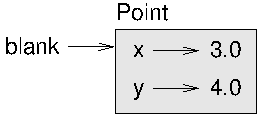
\includegraphics[scale=0.8]{figs/point.pdf}}
\caption{Object diagram.}
\label{fig.point}
\end{figure}


The variable {\tt blank} refers to a Point object, which
contains two attributes.  Each attribute refers to a
floating-point number.

You can read the value of an attribute using the same syntax:

\begin{verbatim}
>>> print blank.y
4.0
>>> x = blank.x
>>> print x
3.0
\end{verbatim}
%
The expression {\tt blank.x} means, ``Go to the object {\tt blank}
refers to and get the value of {\tt x}.'' In this case, we assign that
value to a variable named {\tt x}.  There is no conflict between
the variable {\tt x} and the attribute {\tt x}.

You can use dot notation as part of any expression.  For example:

\begin{verbatim}
>>> print '(%g, %g)' % (blank.x, blank.y)
(3.0, 4.0)
>>> distance = math.sqrt(blank.x**2 + blank.y**2)
>>> print distance
5.0
\end{verbatim}
%
You can pass an instance as an argument in the usual way.
For example:
\index{instance!as argument}

\begin{verbatim}
def print_point(p):
    print '(%g, %g)' % (p.x, p.y)
\end{verbatim}
%
\verb"print_point" takes a point as an argument and displays it in
mathematical notation.  To invoke it, you can pass {\tt blank} as
an argument:

\begin{verbatim}
>>> print_point(blank)
(3.0, 4.0)
\end{verbatim}
%
Inside the function, {\tt p} is an alias for {\tt blank}, so if
the function modifies {\tt p}, {\tt blank} changes.
\index{aliasing}


\begin{exercise}

Write a function called \verb"distance_between_points" that takes two
Points as arguments and returns the distance between them.

\end{exercise}



\section{Rectangles}
\label{rectangles}

Sometimes it is obvious what the attributes of an object should be,
but other times you have to make decisions.  For example, imagine you
are designing a class to represent rectangles.  What attributes would
you use to specify the location and size of a rectangle?  You can
ignore angle; to keep things simple, assume that the rectangle is
either vertical or horizontal.
\index{representation}

There are at least two possibilities:

\begin{itemize}

\item You could specify one corner of the rectangle
(or the center), the width, and the height.

\item You could specify two opposing corners.

\end{itemize}

At this point it is hard to say whether either is better than
the other, so we'll implement the first one, just as an example.
\index{Rectangle class}
\index{class!Rectangle}

Here is the class definition:

\begin{verbatim}
class Rectangle(object):
    """Represents a rectangle.

    attributes: width, height, corner.
    """
\end{verbatim}
%
The docstring lists the attributes:  {\tt width} and
{\tt height} are numbers; {\tt corner} is a Point object that
specifies the lower-left corner.

To represent a rectangle, you have to instantiate a Rectangle
object and assign values to the attributes:

\begin{verbatim}
box = Rectangle()
box.width = 100.0
box.height = 200.0
box.corner = Point()
box.corner.x = 0.0
box.corner.y = 0.0
\end{verbatim}
%
The expression {\tt box.corner.x} means,
``Go to the object {\tt box} refers to and select the attribute named
{\tt corner}; then go to that object and select the attribute named
{\tt x}.''

\begin{figure}
\centerline
{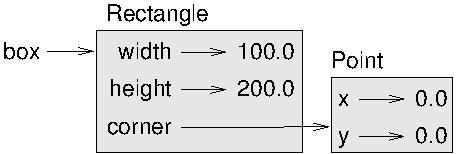
\includegraphics[scale=0.8]{figs/rectangle.pdf}}
\caption{Object diagram.}
\label{fig.rectangle}
\end{figure}


Figure~\ref{fig.rectangle} shows the state of this object.
\index{state diagram}
\index{diagram!state}
\index{object diagram}
\index{diagram!object}
An object that is an attribute of another object is {\bf embedded}.
\index{embedded object}
\index{object!embedded}


\section{Instances as return values}
\index{instance!as return value}
\index{return value}

Functions can return instances.  For example, \verb"find_center"
takes a {\tt Rectangle} as an argument and returns a {\tt Point}
that contains the coordinates of the center of the {\tt Rectangle}:

\begin{verbatim}
def find_center(rect):
    p = Point()
    p.x = rect.corner.x + rect.width/2.0
    p.y = rect.corner.y + rect.height/2.0
    return p
\end{verbatim}
%
Here is an example that passes {\tt box} as an argument and assigns
the resulting Point to {\tt center}:

\begin{verbatim}
>>> center = find_center(box)
>>> print_point(center)
(50.0, 100.0)
\end{verbatim}
%

\section{Objects are mutable}
\index{object!mutable}
\index{mutability}

You can change the state of an object by making an assignment to one of
its attributes.  For example, to change the size of a rectangle
without changing its position, you can modify the values of {\tt
width} and {\tt height}:

\begin{verbatim}
box.width = box.width + 50
box.height = box.width + 100
\end{verbatim}
%
You can also write functions that modify objects.  For example,
\verb"grow_rectangle" takes a Rectangle object and two numbers,
{\tt dwidth} and {\tt dheight}, and adds the numbers to the
width and height of the rectangle:

\begin{verbatim}
def grow_rectangle(rect, dwidth, dheight):
    rect.width += dwidth
    rect.height += dheight
\end{verbatim}
%
Here is an example that demonstrates the effect:

\begin{verbatim}
>>> print box.width
100.0
>>> print box.height
200.0
>>> grow_rectangle(box, 50, 100)
>>> print box.width
150.0
>>> print box.height
300.0
\end{verbatim}
%
Inside the function, {\tt rect} is an
alias for {\tt box}, so if the function modifies {\tt rect},
{\tt box} changes.

\begin{exercise}

Write a function named \verb"move_rectangle" that takes
a Rectangle and two numbers named {\tt dx} and {\tt dy}.  It
should change the location of the rectangle by adding {\tt dx}
to the {\tt x} coordinate of {\tt corner} and adding {\tt dy}
to the {\tt y} coordinate of {\tt corner}.

\end{exercise}


\section{Copying}
\label{copying}
\index{aliasing}

Aliasing can make a program difficult to read because changes
in one place might have unexpected effects in another place.
It is hard to keep track of all the variables that might refer
to a given object.
\index{copying objects}
\index{object!copying}
\index{copy module}
\index{module!copy}

Copying an object is often an alternative to aliasing.
The {\tt copy} module contains a function called {\tt copy} that
can duplicate any object:

\begin{verbatim}
>>> p1 = Point()
>>> p1.x = 3.0
>>> p1.y = 4.0

>>> import copy
>>> p2 = copy.copy(p1)
\end{verbatim}
%
{\tt p1} and {\tt p2} contain the same data, but they are
not the same Point.

\begin{verbatim}
>>> print_point(p1)
(3.0, 4.0)
>>> print_point(p2)
(3.0, 4.0)
>>> p1 is p2
False
>>> p1 == p2
False
\end{verbatim}
%
The {\tt is} operator indicates that {\tt p1} and {\tt p2} are not the
same object, which is what we expected.  But you might have expected
{\tt ==} to yield {\tt True} because these points contain the same
data.  In that case, you will be disappointed to learn that for
instances, the default behavior of the {\tt ==} operator is the same
as the {\tt is} operator; it checks object identity, not object
equivalence.  This behavior can be changed---we'll see how later.
\index{is operator}
\index{operator!is}

If you use {\tt copy.copy} to duplicate a Rectangle, you will find
that it copies the Rectangle object but not the embedded Point.
\index{embedded object!copying}

\begin{verbatim}
>>> box2 = copy.copy(box)
>>> box2 is box
False
>>> box2.corner is box.corner
True
\end{verbatim}

\begin{figure}
\centerline
{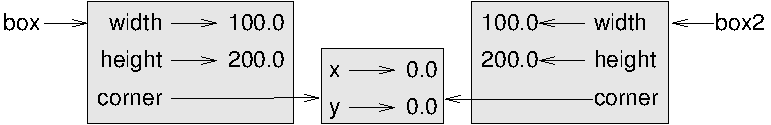
\includegraphics[scale=0.8]{figs/rectangle2.pdf}}
\caption{Object diagram.}
\label{fig.rectangle2}
\end{figure}

Figure~\ref{fig.rectangle2} shows what the object diagram looks like.
\index{state diagram}
\index{diagram!state}
\index{object diagram}
\index{diagram!object}
This operation is called a {\bf shallow copy} because it copies the
object and any references it contains, but not the embedded objects.
\index{shallow copy}
\index{copy!shallow}

For most applications, this is not what you want.  In this example,
invoking \verb"grow_rectangle" on one of the Rectangles would not
affect the other, but invoking \verb"move_rectangle" on either would
affect both!  This behavior is confusing and error-prone.
\index{deep copy}
\index{copy!deep}

Fortunately, the {\tt copy} module contains a method named {\tt
deepcopy} that copies not only the object but also
the objects it refers to, and the objects {\em they} refer to,
and so on.
You will not be surprised to learn that this operation is
called a {\bf deep copy}.
\index{deepcopy function}
\index{function!deepcopy}

\begin{verbatim}
>>> box3 = copy.deepcopy(box)
>>> box3 is box
False
>>> box3.corner is box.corner
False
\end{verbatim}
%
{\tt box3} and {\tt box} are completely separate objects.


\begin{exercise}

Write a version of \verb"move_rectangle" that creates and
returns a new Rectangle instead of modifying the old one.

\end{exercise}


\section{Debugging}
\label{hasattr}
\index{debugging}

When you start working with objects, you are likely to encounter
some new exceptions.  If you try to access an attribute
that doesn't exist, you get an {\tt AttributeError}:
\index{exception!AttributeError}
\index{AttributeError}

\begin{verbatim}
>>> p = Point()
>>> print p.z
AttributeError: Point instance has no attribute 'z'
\end{verbatim}
%
If you are not sure what type an object is, you can ask:
\index{type function}
\index{function!type}

\begin{verbatim}
>>> type(p)
<type '__main__.Point'>
\end{verbatim}
%
If you are not sure whether an object has a particular attribute,
you can use the built-in function {\tt hasattr}:
\index{hasattr function}
\index{function!hasattr}

\begin{verbatim}
>>> hasattr(p, 'x')
True
>>> hasattr(p, 'z')
False
\end{verbatim}
%
The first argument can be any object; the second argument is a {\em
string} that contains the name of the attribute.


\section{Glossary}

\begin{description}

\item[class:] A user-defined type.  A class definition creates a new
class object.
\index{class}

\item[class object:] An object that contains information about a
user-defined type.  The class object can be used to create instances
of the type.
\index{class object}
\index{object!class}

\item[instance:] An object that belongs to a class.
\index{instance}

\item[attribute:] One of the named values associated with an object.
\index{attribute!instance}
\index{instance attribute}

\item[embedded (object):] An object that is stored as an attribute
of another object.
\index{embedded object}
\index{object!embedded}

\item[shallow copy:] To copy the contents of an object, including
any references to embedded objects;
implemented by the {\tt copy} function in the {\tt copy} module.
\index{shallow copy}

\item[deep copy:] To copy the contents of an object as well as any
embedded objects, and any objects embedded in them, and so on;
implemented by the {\tt deepcopy} function in the {\tt copy} module.
\index{deep copy}

\item[object diagram:] A diagram that shows objects, their
attributes, and the values of the attributes.
\index{object diagram}
\index{diagram!object}

\end{description}


\section{Exercises}

\begin{exercise}
\label{canvas}
\index{Swampy}
\index{World module}
\index{module!World}

Swampy (see Chapter~\ref{turtlechap}) provides a module named {\tt
  World}, which defines a user-defined type also called {\tt World}.
You can import it like this:

\begin{verbatim}
from swampy.World import World
\end{verbatim}

Or, depending on how you installed Swampy, like this:

\begin{verbatim}
from World import World
\end{verbatim}

The following code creates a World object and calls
the {\tt mainloop} method, which
waits for the user.

\begin{verbatim}
world = World()
world.mainloop()
\end{verbatim}

A window should appear with a title bar and an empty square.
We will use this window to draw Points,
Rectangles and other shapes.
Add the following lines before calling
\verb"mainloop" and run the program again.
\index{Canvas object}
\index{object!Canvas}

\begin{verbatim}
canvas = world.ca(width=500, height=500, background='white')
bbox = [[-150,-100], [150, 100]]
canvas.rectangle(bbox, outline='black', width=2, fill='green4')
\end{verbatim}

You should see a green rectangle with a black outline.
The first line creates a Canvas, which appears in the window
as a white square.  The Canvas object provides methods like
{\tt rectangle} for drawing various shapes.
\index{bounding box}

{\tt bbox} is a list of lists that represents the ``bounding box''
of the rectangle.  The first pair of coordinates is the lower-left
corner of the rectangle; the second pair is the upper-right corner.

You can draw a circle like this:

\begin{verbatim}
canvas.circle([-25,0], 70, outline=None, fill='red')
\end{verbatim}

The first parameter is the coordinate pair for the center of the
circle; the second parameter is the radius.

If you add this line to the program,
the result should resemble the national flag of Bangladesh
(see \url{http://en.wikipedia.org/wiki/Gallery_of_sovereign-state_flags}).
\index{Bangladesh, national flag}

\begin{enumerate}

\item Write a function called \verb"draw_rectangle" that takes a
  Canvas and a Rectangle as arguments and draws a
  representation of the Rectangle on the Canvas.

\item Add an attribute named {\tt color} to your Rectangle objects and
  modify \verb"draw_rectangle" so that it uses the color attribute as
  the fill color.

\item Write a function called \verb"draw_point" that takes a
  Canvas and a Point as arguments and draws a
  representation of the Point on the Canvas.

\item Define a new class called Circle with appropriate attributes and
  instantiate a few Circle objects.  Write a function called
  \verb"draw_circle" that draws circles on the canvas.
\index{Czech Republic, national flag}

\item Write a program that draws the national flag of the Czech Republic.
Hint: you can draw a polygon like this:

\begin{verbatim}
points = [[-150,-100], [150, 100], [150, -100]]
canvas.polygon(points, fill='blue')
\end{verbatim}

\end{enumerate}
\index{color list}
\index{available colors}

I have written a small program that lists the available colors;
you can download it from \url{http://thinkpython.com/code/color_list.py}.

\end{exercise}


\chapter{Classes and functions}
\label{time}

Code examples from this chapter are available from
\url{http://thinkpython.com/code/Time1.py}.

\section{Time}
\label{time.object}

As another example of a user-defined type, we'll define a class called
{\tt Time} that records the time of day.  The class definition looks
like this:
\index{user-defined type}
\index{type!user-defined}
\index{Time class}
\index{class!Time}

\begin{verbatim}
class Time(object):
    """Represents the time of day.

    attributes: hour, minute, second
    """
\end{verbatim}
%
We can create a new {\tt Time} object and assign
attributes for hours, minutes, and seconds:

\begin{verbatim}
time = Time()
time.hour = 11
time.minute = 59
time.second = 30
\end{verbatim}
%
The state diagram for the {\tt Time} object looks like Figure~\ref{fig.time}.
\index{state diagram}
\index{diagram!state}
\index{object diagram}
\index{diagram!object}

\begin{exercise}
\label{ex.printtime}

Write a function called \verb"print_time" that takes a
Time object and prints it in the form {\tt hour:minute:second}.
Hint: the format sequence \verb"'%.2d'" prints an integer using
at least two digits, including a leading zero if necessary.

\end{exercise}

\begin{exercise}
\label{isafter}
\index{boolean function}

Write a boolean function called \verb"is_after" that
takes two Time objects, {\tt t1} and {\tt t2}, and
returns {\tt True} if {\tt t1} follows {\tt t2} chronologically and
{\tt False} otherwise.  Challenge: don't use an {\tt if} statement.
\end{exercise}

\begin{figure}
\centerline
{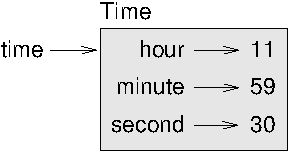
\includegraphics[scale=0.8]{figs/time.pdf}}
\caption{Object diagram.}
\label{fig.time}
\end{figure}


\section{Pure functions}
\index{prototype and patch}
\index{development plan!prototype and patch}

In the next few sections, we'll write two functions that add time
values.  They demonstrate two kinds of functions: pure functions and
modifiers.  They also demonstrate a development plan I'll call {\bf
  prototype and patch}, which is a way of tackling a complex problem
by starting with a simple prototype and incrementally dealing with the
complications.

Here is a simple prototype of \verb"add_time":

\begin{verbatim}
def add_time(t1, t2):
    sum = Time()
    sum.hour = t1.hour + t2.hour
    sum.minute = t1.minute + t2.minute
    sum.second = t1.second + t2.second
    return sum
\end{verbatim}
%
The function creates a new {\tt Time} object, initializes its
attributes, and returns a reference to the new object.  This is called
a {\bf pure function} because it does not modify any of the objects
passed to it as arguments and it has no effect,
like displaying a value or getting user input,
other than returning a value.
\index{pure function}
\index{function type!pure}

To test this function, I'll create two Time objects: {\tt start}
contains the start time of a movie, like {\em Monty Python and the
Holy Grail}, and {\tt duration} contains the run time of the movie,
which is one hour 35 minutes.
\index{Monty Python and the Holy Grail}

\verb"add_time" figures out when the movie will be done.

\begin{verbatim}
>>> start = Time()
>>> start.hour = 9
>>> start.minute = 45
>>> start.second =  0

>>> duration = Time()
>>> duration.hour = 1
>>> duration.minute = 35
>>> duration.second = 0

>>> done = add_time(start, duration)
>>> print_time(done)
10:80:00
\end{verbatim}
%
The result, {\tt 10:80:00} might not be what you were hoping
for.  The problem is that this function does not deal with cases where the
number of seconds or minutes adds up to more than sixty.  When that
happens, we have to ``carry'' the extra seconds into the minute column
or the extra minutes into the hour column.
\index{carrying, addition with}

Here's an improved version:

\begin{verbatim}
def add_time(t1, t2):
    sum = Time()
    sum.hour = t1.hour + t2.hour
    sum.minute = t1.minute + t2.minute
    sum.second = t1.second + t2.second

    if sum.second >= 60:
        sum.second -= 60
        sum.minute += 1

    if sum.minute >= 60:
        sum.minute -= 60
        sum.hour += 1

    return sum
\end{verbatim}
%
Although this function is correct, it is starting to get big.
We will see a shorter alternative later.


\section{Modifiers}
\label{increment}
\index{modifier}
\index{function type!modifier}

Sometimes it is useful for a function to modify the objects it gets as
parameters.  In that case, the changes are visible to the caller.
Functions that work this way are called {\bf modifiers}.
\index{increment}

{\tt increment}, which adds a given number of seconds to a {\tt Time}
object, can be written naturally as a
modifier.  Here is a rough draft:

\begin{verbatim}
def increment(time, seconds):
    time.second += seconds

    if time.second >= 60:
        time.second -= 60
        time.minute += 1

    if time.minute >= 60:
        time.minute -= 60
        time.hour += 1
\end{verbatim}
%
The first line performs the basic operation; the remainder deals
with the special cases we saw before.
\index{special case}

Is this function correct?  What happens if the parameter {\tt seconds}
is much greater than sixty?

In that case, it is not enough to carry
once; we have to keep doing it until {\tt time.second} is less than sixty.
One solution is to replace the {\tt if} statements with {\tt while}
statements.  That would make the function correct, but not
very efficient.

\begin{exercise}

Write a correct version of {\tt increment} that
doesn't contain any loops.

\end{exercise}

Anything that can be done with modifiers can also be done with pure
functions.  In fact, some programming languages only allow pure
functions.  There is some evidence that programs that use pure
functions are faster to develop and less error-prone than programs
that use modifiers.  But modifiers are convenient at times,
and functional programs tend to be less efficient.

In general, I recommend that you write pure functions whenever it is
reasonable and resort to modifiers only if there is a compelling
advantage.  This approach might be called a {\bf functional
programming style}.
\index{functional programming style}


\begin{exercise}

Write a ``pure'' version of {\tt increment} that creates and returns
a new Time object rather than modifying the parameter.

\end{exercise}


\section{Prototyping versus planning}
\label{prototype}
\index{prototype and patch}
\index{development plan!prototype and patch}
\index{planned development}
\index{development plan!planned}

The development plan I am demonstrating is called ``prototype and
patch.''  For each function, I wrote a prototype that performed the
basic calculation and then tested it, patching errors along the
way.

This approach can be effective, especially if you don't yet have a
deep understanding of the problem.  But incremental corrections can
generate code that is unnecessarily complicated---since it deals with
many special cases---and unreliable---since it is hard to know if you
have found all the errors.

An alternative is {\bf planned development}, in which high-level
insight into the problem can make the programming much easier.  In
this case, the insight is that a Time object is really a three-digit
number in base 60 (see \url{http://en.wikipedia.org/wiki/Sexagesimal}.)!  The
{\tt second} attribute is the ``ones column,'' the {\tt minute}
attribute is the ``sixties column,'' and the {\tt hour} attribute is
the ``thirty-six hundreds column.''
\index{sexagesimal}

When we wrote \verb"add_time" and {\tt increment}, we were effectively
doing addition in base 60, which is why we had to carry from one
column to the next.
\index{carrying, addition with}

This observation suggests another approach to the whole problem---we
can convert Time objects to integers and take advantage of the fact
that the computer knows how to do integer arithmetic.

Here is a function that converts Times to integers:

\begin{verbatim}
def time_to_int(time):
    minutes = time.hour * 60 + time.minute
    seconds = minutes * 60 + time.second
    return seconds
\end{verbatim}
%
And here is the function that converts integers to Times
(recall that {\tt divmod} divides the first argument by the second
and returns the quotient and remainder as a tuple).
\index{divmod}

\begin{verbatim}
def int_to_time(seconds):
    time = Time()
    minutes, time.second = divmod(seconds, 60)
    time.hour, time.minute = divmod(minutes, 60)
    return time
\end{verbatim}
%
You might have to think a bit, and run some tests, to convince
yourself that these functions are correct.  One way to test them is to
check that \verb"time_to_int(int_to_time(x)) == x" for many values of
{\tt x}.  This is an example of a consistency check.
\index{consistency check}

Once you are convinced they are correct, you can use them to
rewrite \verb"add_time":

\begin{verbatim}
def add_time(t1, t2):
    seconds = time_to_int(t1) + time_to_int(t2)
    return int_to_time(seconds)
\end{verbatim}
%
This version is shorter than the original, and easier to verify.

\begin{exercise}

Rewrite {\tt increment} using \verb"time_to_int" and \verb"int_to_time".

\end{exercise}

In some ways, converting from base 60 to base 10 and back is harder
than just dealing with times.  Base conversion is more abstract; our
intuition for dealing with time values is better.

But if we have the insight to treat times as base 60 numbers and make
the investment of writing the conversion functions (\verb"time_to_int"
and \verb"int_to_time"), we get a program that is shorter, easier to
read and debug, and more reliable.

It is also easier to add features later.  For example, imagine
subtracting two Times to find the duration between them.  The
naive approach would be to implement subtraction with borrowing.
Using the conversion functions would be easier and more likely to be
correct.
\index{subtraction with borrowing}
\index{borrowing, subtraction with}
\index{generalization}

Ironically, sometimes making a problem harder (or more general) makes it
easier (because there are fewer special cases and fewer opportunities
for error).


\section{Debugging}
\index{debugging}

A Time object is well-formed if the values of {\tt minute} and {\tt
second} are between 0 and 60 (including 0 but not 60) and if
{\tt hour} is positive.  {\tt hour} and {\tt minute} should be
integral values, but we might allow {\tt second} to have a
fraction part.
\index{invariant}

Requirements like these are called {\bf invariants} because
they should always be true.  To put it a different way, if they
are not true, then something has gone wrong.

Writing code to check your invariants can help you detect errors
and find their causes.  For example, you might have a function
like \verb"valid_time" that takes a Time object and returns
{\tt False} if it violates an invariant:

\begin{verbatim}
def valid_time(time):
    if time.hour < 0 or time.minute < 0 or time.second < 0:
        return False
    if time.minute >= 60 or time.second >= 60:
        return False
    return True
\end{verbatim}
%
Then at the beginning of each function you could check the
arguments to make sure they are valid:
\index{raise statement}
\index{statement!raise}

\begin{verbatim}
def add_time(t1, t2):
    if not valid_time(t1) or not valid_time(t2):
        raise ValueError, 'invalid Time object in add_time'
    seconds = time_to_int(t1) + time_to_int(t2)
    return int_to_time(seconds)
\end{verbatim}
%
Or you could use an {\tt assert} statement, which checks a given invariant
and raises an exception if it fails:
\index{assert statement}
\index{statement!assert}

\begin{verbatim}
def add_time(t1, t2):
    assert valid_time(t1) and valid_time(t2)
    seconds = time_to_int(t1) + time_to_int(t2)
    return int_to_time(seconds)
\end{verbatim}
%
{\tt assert} statements are useful because they distinguish
code that deals with normal conditions from code
that checks for errors.


\section{Glossary}

\begin{description}

\item[prototype and patch:] A development plan that involves
writing a rough draft of a program, testing, and correcting errors as
they are found.
\index{prototype and patch}

\item[planned development:] A development plan that involves
high-level insight into the problem and more planning than incremental
development or prototype development.
\index{planned development}

\item[pure function:] A function that does not modify any of the objects it
receives as arguments.  Most pure functions are fruitful.
\index{pure function}

\item[modifier:] A function that changes one or more of the objects it
receives as arguments.  Most modifiers are fruitless.
\index{modifier}

\item[functional programming style:] A style of program design in which the
majority of functions are pure.
\index{functional programming style}

\item[invariant:] A condition that should always be true during the
execution of a program.
\index{invariant}

\end{description}


\section{Exercises}

Code examples from this chapter are available from
\url{http://thinkpython.com/code/Time1.py}; solutions to these
exercises are available from \url{http://thinkpython.com/code/Time1_soln.py}.

\begin{exercise}

Write a function called \verb"mul_time" that takes a Time object
and a number and returns a new Time object that contains
the product of the original Time and the number.

Then use \verb"mul_time" to write a function that takes a Time
object that represents the finishing time in a race, and a number
that represents the distance, and returns a Time object that represents
the average pace (time per mile).
\index{running pace}

\end{exercise}

%\begin{exercise}
%\index{Date class}
%\index{class!Date}

%Write a class definition for a Date object that has attributes {\tt
%  day}, {\tt month} and {\tt year}.  Write a function called
%\verb"increment_date" that takes a Date object, {\tt date} and an
%integer, {\tt n}, and returns a new Date object that
%represents the day {\tt n} days after {\tt date}.  Hint:
%``Thirty days hath September...''  Challenge: does your function
%deal with leap years correctly?  See \url{http://en.wikipedia.org/wiki/Leap_year}.

%\end{exercise}


\begin{exercise}
\index{datetime module}
\index{module!datetime}

The {\tt datetime} module provides {\tt date} and {\tt time} objects
that are similar to the Date and Time objects in this chapter, but
they provide a rich set of methods and operators.  Read the
documentation at \url{http://docs.python.org/2/library/datetime.html}.

\begin{enumerate}

\item Use the {\tt datetime} module to write a program that gets the
  current date and prints the day of the week.
\index{birthday}

\item Write a program that takes a birthday as input and prints the
  user's age and the number of days, hours, minutes and seconds until
  their next birthday.

\item For two people born on different days, there is a day when one
  is twice as old as the other. That's their Double Day.  Write a
  program that takes two birthdays and computes their Double Day.

\item For a little more challenge, write the more general version that
  computes the day when one person is $n$ times older than the other.
\index{Double Day}

\end{enumerate}

\end{exercise}


\chapter{Classes and methods}

Code examples from this chapter are available from
\url{http://thinkpython.com/code/Time2.py}.

\section{Object-oriented features}
\index{object-oriented programming}

Python is an {\bf object-oriented programming language}, which means
that it provides features that support object-oriented
programming.

It is not easy to define object-oriented programming, but we have
already seen some of its characteristics:

\begin{itemize}

\item Programs are made up of object definitions and function
definitions, and most of the computation is expressed in terms
of operations on objects.

\item Each object definition corresponds to some object or concept
in the real world, and the functions that operate on that object
correspond to the ways real-world objects interact.

\end{itemize}

For example, the {\tt Time} class defined in Chapter~\ref{time}
corresponds to the way people record the time of day, and the
functions we defined correspond to the kinds of things people do with
times.  Similarly, the {\tt Point} and {\tt Rectangle} classes
correspond to the mathematical concepts of a point and a rectangle.

So far, we have not taken advantage of the features Python provides to
support object-oriented programming.  These
features are not strictly necessary; most of them provide
alternative syntax for things we have already done.  But in many cases,
the alternative is more concise and more accurately conveys the
structure of the program.

For example, in the {\tt Time} program, there is no obvious
connection between the class definition and the function definitions
that follow.  With some examination, it is apparent that every function
takes at least one {\tt Time} object as an argument.
\index{method}
\index{function}

This observation is the motivation for {\bf methods}; a method is
a function that is associated with a particular class.
We have seen methods for strings, lists, dictionaries and tuples.
In this chapter, we will define methods for user-defined types.
\index{syntax}
\index{semantics}

Methods are semantically the same as functions, but there are
two syntactic differences:

\begin{itemize}

\item Methods are defined inside a class definition in order
to make the relationship between the class and the method explicit.

\item The syntax for invoking a method is different from the
syntax for calling a function.

\end{itemize}

In the next few sections, we will take the functions from the previous
two chapters and transform them into methods.  This transformation is
purely mechanical; you can do it simply by following a sequence of
steps.  If you are comfortable converting from one form to another,
you will be able to choose the best form for whatever you are doing.


\section{Printing objects}
\index{object!printing}

In Chapter~\ref{time}, we defined a class named
{\tt Time} and in Exercise~\ref{ex.printtime}, you
wrote a function named \verb"print_time":

\begin{verbatim}
class Time(object):
    """Represents the time of day."""

def print_time(time):
    print '%.2d:%.2d:%.2d' % (time.hour, time.minute, time.second)
\end{verbatim}
%
To call this function, you have to pass a {\tt Time} object as an
argument:

\begin{verbatim}
>>> start = Time()
>>> start.hour = 9
>>> start.minute = 45
>>> start.second = 00
>>> print_time(start)
09:45:00
\end{verbatim}
%
To make \verb"print_time" a method, all we have to do is
move the function definition inside the class definition.  Notice
the change in indentation.
\index{indentation}

\begin{verbatim}
class Time(object):
    def print_time(time):
        print '%.2d:%.2d:%.2d' % (time.hour, time.minute, time.second)
\end{verbatim}
%
Now there are two ways to call \verb"print_time".  The first
(and less common) way is to use function syntax:
\index{function syntax}
\index{dot notation}


\begin{verbatim}
>>> Time.print_time(start)
09:45:00
\end{verbatim}
%
In this use of dot notation, {\tt Time} is the name of the class,
and \verb"print_time" is the name of the method.  {\tt start} is
passed as a parameter.

The second (and more concise) way is to use method syntax:
\index{method syntax}

\begin{verbatim}
>>> start.print_time()
09:45:00
\end{verbatim}
%
In this use of dot notation, \verb"print_time" is the name of the
method (again), and {\tt start} is the object the method is
invoked on, which is called the {\bf subject}.  Just as the
subject of a sentence is what the sentence is about, the subject
of a method invocation is what the method is about.
\index{subject}

Inside the method, the subject is assigned to the first
parameter, so in this case {\tt start} is assigned
to {\tt time}.
\index{self (parameter name)}
\index{parameter!self}

By convention, the first parameter of a method is
called {\tt self}, so it would be more common to write
\verb"print_time" like this:

\begin{verbatim}
class Time(object):
    def print_time(self):
        print '%.2d:%.2d:%.2d' % (self.hour, self.minute, self.second)
\end{verbatim}
%
The reason for this convention is an implicit metaphor:
\index{metaphor, method invocation}

\begin{itemize}

\item The syntax for a function call, \verb"print_time(start)",
  suggests that the function is the active agent.  It says something
  like, ``Hey \verb"print_time"!  Here's an object for you to print.''

\item In object-oriented programming, the objects are the active
  agents.  A method invocation like \verb"start.print_time()" says
  ``Hey {\tt start}!  Please print yourself.''

\end{itemize}

This change in perspective might be more polite, but it is not obvious
that it is useful.  In the examples we have seen so far, it may not
be.  But sometimes shifting responsibility from the functions onto the
objects makes it possible to write more versatile functions, and makes
it easier to maintain and reuse code.

\begin{exercise}
\label{convert}

Rewrite \verb"time_to_int" (from Section~\ref{prototype}) as a method.
It is probably not appropriate to rewrite \verb"int_to_time" as a
method; what object you would invoke it on?

\end{exercise}


\section{Another example}
\index{increment}

Here's a version of {\tt increment} (from Section~\ref{increment})
rewritten as a method:

\begin{verbatim}
# inside class Time:

    def increment(self, seconds):
        seconds += self.time_to_int()
        return int_to_time(seconds)
\end{verbatim}
%
This version assumes that \verb"time_to_int" is written
as a method, as in Exercise~\ref{convert}.  Also, note that
it is a pure function, not a modifier.

Here's how you would invoke {\tt increment}:

\begin{verbatim}
>>> start.print_time()
09:45:00
>>> end = start.increment(1337)
>>> end.print_time()
10:07:17
\end{verbatim}
%
The subject, {\tt start}, gets assigned to the first parameter,
{\tt self}.  The argument, {\tt 1337}, gets assigned to the
second parameter, {\tt seconds}.

This mechanism can be confusing, especially if you make an error.
For example, if you invoke {\tt increment} with two arguments, you
get:
\index{exception!TypeError}
\index{TypeError}

\begin{verbatim}
>>> end = start.increment(1337, 460)
TypeError: increment() takes exactly 2 arguments (3 given)
\end{verbatim}
%
The error message is initially confusing, because there are
only two arguments in parentheses.  But the subject is also
considered an argument, so all together that's three.


\section{A more complicated example}

\verb"is_after" (from Exercise~\ref{isafter}) is slightly more complicated
because it takes two Time objects as parameters.  In this case it is
conventional to name the first parameter {\tt self} and the second
parameter {\tt other}:
\index{other (parameter name)}
\index{parameter!other}

\begin{verbatim}
# inside class Time:

    def is_after(self, other):
        return self.time_to_int() > other.time_to_int()
\end{verbatim}
%
To use this method, you have to invoke it on one object and pass
the other as an argument:

\begin{verbatim}
>>> end.is_after(start)
True
\end{verbatim}
%
One nice thing about this syntax is that it almost reads
like English: ``end is after start?''


\section{The init method}
\index{init method}
\index{method!init}

The init method (short for ``initialization'') is
a special method that gets invoked when an object is instantiated.
Its full name is \verb"__init__" (two underscore characters,
followed by {\tt init}, and then two more underscores).  An
init method for the {\tt Time} class might look like this:

\begin{verbatim}
# inside class Time:

    def __init__(self, hour=0, minute=0, second=0):
        self.hour = hour
        self.minute = minute
        self.second = second
\end{verbatim}
%
It is common for the parameters of \verb"__init__"
to have the same names as the attributes.  The statement

\begin{verbatim}
        self.hour = hour
\end{verbatim}
%
stores the value of the parameter {\tt hour} as an attribute
of {\tt self}.
\index{optional parameter}
\index{parameter!optional}
\index{default value}
\index{override}

The parameters are optional, so if you call {\tt Time} with
no arguments, you get the default values.

\begin{verbatim}
>>> time = Time()
>>> time.print_time()
00:00:00
\end{verbatim}
%
If you provide one argument, it overrides {\tt hour}:

\begin{verbatim}
>>> time = Time (9)
>>> time.print_time()
09:00:00
\end{verbatim}
%
If you provide two arguments, they override {\tt hour} and
{\tt minute}.

\begin{verbatim}
>>> time = Time(9, 45)
>>> time.print_time()
09:45:00
\end{verbatim}
%
And if you provide three arguments, they override all three
default values.


\begin{exercise}
\index{Point class}
\index{class!Point}

Write an init method for the {\tt Point} class that takes
{\tt x} and {\tt y} as optional parameters and assigns
them to the corresponding attributes.
\end{exercise}


\section{The {\tt \_\_str\_\_} method}
\index{str method@\_\_str\_\_ method}
\index{method!\_\_str\_\_}

\verb"__str__" is a special method, like \verb"__init__",
that is supposed to return a string representation of an object.
\index{string representation}

For example, here is a {\tt str} method for Time objects:

\begin{verbatim}
# inside class Time:

    def __str__(self):
        return '%.2d:%.2d:%.2d' % (self.hour, self.minute, self.second)
\end{verbatim}
%
When you {\tt print} an object, Python invokes the {\tt str} method:
\index{print statement}
\index{statement!print}

\begin{verbatim}
>>> time = Time(9, 45)
>>> print time
09:45:00
\end{verbatim}
%
When I write a new class, I almost always start by writing
\verb"__init__", which makes it easier to instantiate objects, and
\verb"__str__", which is useful for debugging.


\begin{exercise}

Write a {\tt str} method for the {\tt Point} class.  Create
a Point object and print it.

\end{exercise}


\section{Operator overloading}
\label{operator.overloading}

By defining other special methods, you can specify the behavior
of operators on user-defined types.  For example, if you define
a method named \verb"__add__" for the {\tt Time} class, you can use the
{\tt +} operator on Time objects.

Here is what the definition might look like:
\index{add method}
\index{method!add}

\begin{verbatim}
# inside class Time:

    def __add__(self, other):
        seconds = self.time_to_int() + other.time_to_int()
        return int_to_time(seconds)
\end{verbatim}
%
And here is how you could use it:

\begin{verbatim}
>>> start = Time(9, 45)
>>> duration = Time(1, 35)
>>> print start + duration
11:20:00
\end{verbatim}
%
When you apply the {\tt +} operator to Time objects, Python invokes
\verb"__add__".  When you print the result, Python invokes
\verb"__str__".  So there is quite a lot happening behind the scenes!
\index{operator overloading}

Changing the behavior of an operator so that it works with
user-defined types is called {\bf operator overloading}.  For every
operator in Python there is a corresponding special method, like
\verb"__add__".  For more details, see
\url{http://docs.python.org/2/reference/datamodel.html#specialnames}.

\begin{exercise}

Write an {\tt add} method for the Point class.

\end{exercise}


\section{Type-based dispatch}

In the previous section we added two Time objects, but you
also might want to add an integer to a Time object.  The
following is a version of \verb"__add__"
that checks the type of {\tt other} and invokes either
\verb"add_time" or {\tt increment}:

\begin{verbatim}
# inside class Time:

    def __add__(self, other):
        if isinstance(other, Time):
            return self.add_time(other)
        else:
            return self.increment(other)

    def add_time(self, other):
        seconds = self.time_to_int() + other.time_to_int()
        return int_to_time(seconds)

    def increment(self, seconds):
        seconds += self.time_to_int()
        return int_to_time(seconds)
\end{verbatim}
%
The built-in function {\tt isinstance} takes a value and a
class object, and returns {\tt True} if the value is an instance
of the class.
\index{isinstance function}
\index{function!isinstance}

If {\tt other} is a Time object, \verb"__add__" invokes
\verb"add_time".  Otherwise it assumes that the parameter
is a number and invokes {\tt increment}.  This operation is
called a {\bf type-based dispatch} because it dispatches the
computation to different methods based on the type of the
arguments.
\index{type-based dispatch}
\index{dispatch, type-based}

Here are examples that use the {\tt +} operator with different
types:

\begin{verbatim}
>>> start = Time(9, 45)
>>> duration = Time(1, 35)
>>> print start + duration
11:20:00
>>> print start + 1337
10:07:17
\end{verbatim}
%
Unfortunately, this implementation of addition is not commutative.
If the integer is the first operand, you get
\index{commutativity}

\begin{verbatim}
>>> print 1337 + start
TypeError: unsupported operand type(s) for +: 'int' and 'instance'
\end{verbatim}
%
The problem is, instead of asking the Time object to add an integer,
Python is asking an integer to add a Time object, and it doesn't know
how to do that.  But there is a clever solution for this problem: the
special method \verb"__radd__", which stands for ``right-side add.''
This method is invoked when a Time object appears on the right side of
the {\tt +} operator.  Here's the definition:
\index{radd method}
\index{method!radd}

\begin{verbatim}
# inside class Time:

    def __radd__(self, other):
        return self.__add__(other)
\end{verbatim}
%
And here's how it's used:

\begin{verbatim}
>>> print 1337 + start
10:07:17
\end{verbatim}
%

\begin{exercise}

Write an {\tt add} method for Points that works with either a
Point object or a tuple:

\begin{itemize}

\item If the second operand is a Point, the method should return a new
Point whose $x$ coordinate is the sum of the $x$ coordinates of the
operands, and likewise for the $y$ coordinates.

\item If the second operand is a tuple, the method should add the
first element of the tuple to the $x$ coordinate and the second
element to the $y$ coordinate, and return a new Point with the result.

\end{itemize}

\end{exercise}

\section{Polymorphism}

Type-based dispatch is useful when it is necessary, but (fortunately)
it is not always necessary.  Often you can avoid it by writing functions
that work correctly for arguments with different types.
\index{type-based dispatch}
\index{dispatch!type-based}

Many of the functions we wrote for strings will actually
work for any kind of sequence.
For example, in Section~\ref{histogram}
we used {\tt histogram} to count the number of times each letter
appears in a word.

\begin{verbatim}
def histogram(s):
    d = dict()
    for c in s:
        if c not in d:
            d[c] = 1
        else:
            d[c] = d[c]+1
    return d
\end{verbatim}
%
This function also works for lists, tuples, and even dictionaries,
as long as the elements of {\tt s} are hashable, so they can be used
as keys in {\tt d}.

\begin{verbatim}
>>> t = ['spam', 'egg', 'spam', 'spam', 'bacon', 'spam']
>>> histogram(t)
{'bacon': 1, 'egg': 1, 'spam': 4}
\end{verbatim}
%
Functions that can work with several types are called {\bf polymorphic}.
Polymorphism can facilitate code reuse.  For example, the built-in
function {\tt sum}, which adds the elements of a sequence, works
as long as the elements of the sequence support addition.
\index{polymorphism}

Since Time objects provide an {\tt add} method, they work
with {\tt sum}:

\begin{verbatim}
>>> t1 = Time(7, 43)
>>> t2 = Time(7, 41)
>>> t3 = Time(7, 37)
>>> total = sum([t1, t2, t3])
>>> print total
23:01:00
\end{verbatim}
%
In general, if all of the operations inside a function
work with a given type, then the function works with that type.

The best kind of polymorphism is the unintentional kind, where
you discover that a function you already wrote can be
applied to a type you never planned for.


\section{Debugging}
\index{debugging}

It is legal to add attributes to objects at any point in the execution
of a program, but if you are a stickler for type theory, it is a
dubious practice to have objects of the same type with different
attribute sets.  It is usually a good idea to
initialize all of an objects attributes in the init method.
\index{init method}
\index{attribute!initializing}

If you are not sure whether an object has a particular attribute, you
can use the built-in function {\tt hasattr} (see Section~\ref{hasattr}).
\index{hasattr function}
\index{function!hasattr}
\index{dict attribute@\_\_dict\_\_ attribute}
\index{attribute!\_\_dict\_\_}

Another way to access the attributes of an object is through the
special attribute \verb"__dict__", which is a dictionary that maps
attribute names (as strings) and values:

\begin{verbatim}
>>> p = Point(3, 4)
>>> print p.__dict__
{'y': 4, 'x': 3}
\end{verbatim}
%
For purposes of debugging, you might find it useful to keep this
function handy:

\begin{verbatim}
def print_attributes(obj):
    for attr in obj.__dict__:
        print attr, getattr(obj, attr)
\end{verbatim}
%
\verb"print_attributes" traverses the items in the object's dictionary
and prints each attribute name and its corresponding value.
\index{traversal!dictionary}
\index{dictionary!traversal}

The built-in function {\tt getattr} takes an object and an attribute
name (as a string) and returns the attribute's value.
\index{getattr function}
\index{function!getattr}


\section{Interface and implementation}

One of the goals of object-oriented design is to make software more
maintainable, which means that you can keep the program working when
other parts of the system change, and modify the program to meet new
requirements.
\index{interface}
\index{implementation}
\index{maintainable}
\index{object-oriented design}

A design principle that helps achieve that goal is to keep
interfaces separate from implementations.  For objects, that means
that the methods a class provides should not depend on how the
attributes are represented.
\index{attribute}

For example, in this chapter we developed a class that represents
a time of day.  Methods provided by this class include
\verb"time_to_int", \verb"is_after", and \verb"add_time".

We could implement those methods in several ways.  The details of the
implementation depend on how we represent time.  In this chapter, the
attributes of a {\tt Time} object are {\tt hour}, {\tt minute}, and
{\tt second}.

As an alternative, we could replace these attributes with
a single integer representing the number of seconds
since midnight.  This implementation would make some methods,
like \verb"is_after", easier to write, but it makes some methods
harder.

After you deploy a new class, you might discover a better
implementation.  If other parts of the program are using your
class, it might be time-consuming and error-prone to change the
interface.

But if you designed the interface carefully, you can
change the implementation without changing the interface, which
means that other parts of the program don't have to change.

Keeping the interface separate from the implementation means that
you have to hide the attributes.  Code in other parts of the program
(outside the class definition) should use methods to read
and modify the state of the object.  They should not access the
attributes directly.  This principle is called {\bf information hiding};
see \url{http://en.wikipedia.org/wiki/Information_hiding}.
\index{information hiding}

\begin{exercise}

Download the code from this chapter
(\url{http://thinkpython.com/code/Time2.py}).  Change the attributes
of {\tt Time} to be a single integer representing seconds since
midnight.  Then modify the methods (and the function
\verb"int_to_time") to work with the new implementation.  You should
not have to modify the test code in {\tt main}.  When you are done,
the output should be the same as before.  Solution:
\url{http://thinkpython.com/code/Time2_soln.py}

\end{exercise}


\section{Glossary}

\begin{description}

\item[object-oriented language:] A language that provides features,
  such as user-defined classes and method syntax, that facilitate
  object-oriented programming.
\index{object-oriented language}

\item[object-oriented programming:] A style of programming in which
data and the operations that manipulate it are organized into classes
and methods.
\index{object-oriented programming}

\item[method:] A function that is defined inside a class definition and
is invoked on instances of that class.
\index{method}

\item[subject:] The object a method is invoked on.
\index{subject}

\item[operator overloading:] Changing the behavior of an operator like
{\tt +} so it works with a user-defined type.
\index{overloading}
\index{operator!overloading}

\item[type-based dispatch:] A programming pattern that checks the type
of an operand and invokes different functions for different types.
\index{type-based dispatch}

\item[polymorphic:] Pertaining to a function that can work with more
  than one type.
\index{polymorphism}

\item[information hiding:] The principle that the interface provided
by an object should not depend on its implementation, in particular
the representation of its attributes.
\index{information hiding}


\end{description}

\section{Exercises}

\begin{exercise}
\index{default value!avoiding mutable}
\index{mutable object, as default value}
\index{worst bug}
\index{bug!worst}
\index{Kangaroo class}
\index{class!Kangaroo}

This exercise is a cautionary tale about one of the most
common, and difficult to find, errors in Python.
Write a definition for a class named {\tt Kangaroo} with the following
methods:

\begin{enumerate}

\item An \verb"__init__" method that initializes an attribute named
\verb"pouch_contents" to an empty list.

\item A method named \verb"put_in_pouch" that takes an object
of any type and adds it to \verb"pouch_contents".

\item A \verb"__str__" method that returns a string representation
of the Kangaroo object and the contents of the pouch.

\end{enumerate}
%
Test your code
by creating two {\tt Kangaroo} objects, assigning them to variables
named {\tt kanga} and {\tt roo}, and then adding {\tt roo} to the
contents of {\tt kanga}'s pouch.

Download \url{http://thinkpython.com/code/BadKangaroo.py}.  It contains
a solution to the previous problem with one big, nasty bug.
Find and fix the bug.

If you get stuck, you can download
\url{http://thinkpython.com/code/GoodKangaroo.py}, which explains the
problem and demonstrates a solution.
\index{aliasing}
\index{embedded object}
\index{object!embedded}

\end{exercise}




\begin{exercise}
\index{Visual module}
\index{module!Visual}
\index{vpython module}
\index{module!vpython}

Visual is a Python module that provides 3-D graphics.  It is
not always included in a Python installation, so you might have
to install it from your software repository or, if it's not there,
from \url{vpython.org}.

The following example creates a 3-D space that is 256 units
wide, long and high, and sets the ``center'' to be the
point $(128,128,128)$.  Then it draws a blue sphere.

\begin{verbatim}
from visual import *

scene.range = (256, 256, 256)
scene.center = (128, 128, 128)

color = (0.1, 0.1, 0.9)          # mostly blue
sphere(pos=scene.center, radius=128, color=color)
\end{verbatim}

{\tt color} is an RGB tuple; that is, the elements are Red-Green-Blue
levels between 0.0 and 1.0 (see
\url{http://en.wikipedia.org/wiki/RGB_color_model}).

If you run this code, you should see a window with a black
background and a blue sphere.  If you drag the middle button
up and down, you can zoom in and out.  You can also rotate
the scene by dragging the right button, but with only one
sphere in the world, it is hard to tell the difference.

The following loop creates a cube of spheres:

\begin{verbatim}
t = range(0, 256, 51)
for x in t:
    for y in t:
        for z in t:
            pos = x, y, z
            sphere(pos=pos, radius=10, color=color)
\end{verbatim}

\begin{enumerate}

\item Put this code in a script and make sure it works for
you.

\item Modify the program so that each sphere in the cube
has the color that corresponds to its position in RGB space.
Notice that the coordinates are in the range 0--255, but
the RGB tuples are in the range 0.0--1.0.
\index{color list}
\index{available colors}

\item Download \url{http://thinkpython.com/code/color_list.py}
and use the function \verb"read_colors" to generate a list
of the available colors on your system, their names and
RGB values.  For each named color draw a sphere in the
position that corresponds to its RGB values.



\end{enumerate}

You can see my solution at \url{http://thinkpython.com/code/color_space.py}.

\end{exercise}


\chapter{Inheritance}

In this chapter I present classes to represent playing cards,
decks of cards, and poker hands.  If you don't play poker, you can
read about it at \url{http://en.wikipedia.org/wiki/Poker}, but you don't have
to; I'll tell you what you need to know for the exercises.
Code examples from this chapter are available from
\url{http://thinkpython.com/code/Card.py}.
\index{playing card, Anglo-American}
\index{card, playing}
\index{poker}

If you are not familiar with Anglo-American playing cards,
you can read about them at \url{http://en.wikipedia.org/wiki/Playing_cards}.


\section{Card objects}

There are fifty-two cards in a deck, each of which belongs to one of
four suits and one of thirteen ranks.  The suits are Spades, Hearts,
Diamonds, and Clubs (in descending order in bridge).  The ranks are
Ace, 2, 3, 4, 5, 6, 7, 8, 9, 10, Jack, Queen, and King.  Depending on
the game that you are playing, an Ace may be higher than King
or lower than 2.
\index{rank}
\index{suit}

If we want to define a new object to represent a playing card, it is
obvious what the attributes should be: {\tt rank} and
{\tt suit}.  It is not as obvious what type the attributes
should be.  One possibility is to use strings containing words like
\verb"'Spade'" for suits and \verb"'Queen'" for ranks.  One problem with
this implementation is that it would not be easy to compare cards to
see which had a higher rank or suit.
\index{encode}
\index{encrypt}
\index{map to}
\index{representation}

An alternative is to use integers to {\bf encode} the ranks and suits.
In this context, ``encode'' means that we are going to define a mapping
between numbers and suits, or between numbers and ranks.  This
kind of encoding is not meant to be a secret (that
would be ``encryption'').

\newcommand{\mymapsto}{$\mapsto$}

For example, this table shows the suits and the corresponding integer
codes:

\begin{tabular}{l c l}
Spades & \mymapsto & 3 \\
Hearts & \mymapsto & 2 \\
Diamonds & \mymapsto & 1 \\
Clubs & \mymapsto & 0
\end{tabular}

This code makes it easy to compare cards; because higher suits map to
higher numbers, we can compare suits by comparing their codes.

The mapping for ranks is fairly obvious; each of the numerical ranks
maps to the corresponding integer, and for face cards:

\begin{tabular}{l c l}
Jack & \mymapsto & 11 \\
Queen & \mymapsto & 12 \\
King & \mymapsto & 13 \\
\end{tabular}

I am using the \mymapsto~symbol to make it clear that these mappings
are not part of the Python program.  They are part of the program
design, but they don't appear explicitly in the code.
\index{Card class}
\index{class!Card}

The class definition for {\tt Card} looks like this:

\begin{verbatim}
class Card(object):
    """Represents a standard playing card."""

    def __init__(self, suit=0, rank=2):
        self.suit = suit
        self.rank = rank
\end{verbatim}
%
As usual, the init method takes an optional
parameter for each attribute.  The default card is
the 2 of Clubs.
\index{init method}
\index{method!init}

To create a Card, you call {\tt Card} with the
suit and rank of the card you want.

\begin{verbatim}
queen_of_diamonds = Card(1, 12)
\end{verbatim}
%


\section{Class attributes}
\label{class.attribute}
\index{class attribute}
\index{attribute!class}

In order to print Card objects in a way that people can easily
read, we need a mapping from the integer codes to the corresponding
ranks and suits.  A natural way to
do that is with lists of strings.  We assign these lists to {\bf class
attributes}:

\begin{verbatim}
# inside class Card:

    suit_names = ['Clubs', 'Diamonds', 'Hearts', 'Spades']
    rank_names = [None, 'Ace', '2', '3', '4', '5', '6', '7',
              '8', '9', '10', 'Jack', 'Queen', 'King']

    def __str__(self):
        return '%s of %s' % (Card.rank_names[self.rank],
                             Card.suit_names[self.suit])
\end{verbatim}
%
Variables like \verb"suit_names" and \verb"rank_names", which are
defined inside a class but outside of any method, are called
class attributes because they are associated with the class object
{\tt Card}.
\index{instance attribute}
\index{attribute!instance}

This term distinguishes them from variables like {\tt suit} and {\tt
  rank}, which are called {\bf instance attributes} because they are
associated with a particular instance.
\index{dot notation}

Both kinds of attribute are accessed using dot notation.  For
example, in \verb"__str__", {\tt self} is a Card object,
and {\tt self.rank} is its rank.  Similarly, {\tt Card}
is a class object, and \verb"Card.rank_names" is a
list of strings associated with the class.

Every card has its own {\tt suit} and {\tt rank}, but there
is only one copy of \verb"suit_names" and \verb"rank_names".

Putting it all together, the expression
\verb"Card.rank_names[self.rank]" means ``use the attribute {\tt rank}
from the object {\tt self} as an index into the list \verb"rank_names"
from the class {\tt Card}, and select the appropriate string.''

The first element of \verb"rank_names" is {\tt None} because there
is no card with rank zero.  By including {\tt None} as a place-keeper,
we get a mapping with the nice property that the index 2 maps to the
string \verb"'2'", and so on.  To avoid this tweak, we could have
used a dictionary instead of a list.

With the methods we have so far, we can create and print cards:

\begin{verbatim}
>>> card1 = Card(2, 11)
>>> print card1
Jack of Hearts
\end{verbatim}

\begin{figure}
\centerline
{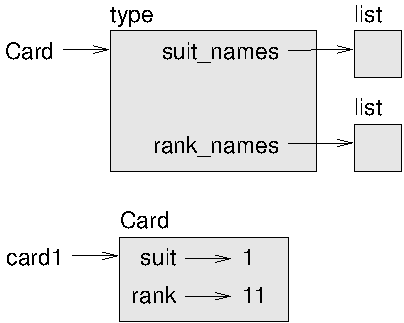
\includegraphics[scale=0.8]{figs/card1.pdf}}
\caption{Object diagram.}
\label{fig.card1}
\end{figure}

Figure~\ref{fig.card1} is a diagram of the {\tt Card} class object
and one Card instance.
\index{state diagram}
\index{diagram!state}
\index{object diagram}
\index{diagram!object}
{\tt Card} is a class object, so it has type {\tt type}.  {\tt
card1} has type {\tt Card}.  (To save space, I didn't draw the
contents of \verb"suit_names" and \verb"rank_names").


\section{Comparing cards}
\label{comparecard}
\index{operator!relational}
\index{relational operator}

For built-in types, there are relational operators
({\tt <}, {\tt >}, {\tt ==}, etc.)
that compare
values and determine when one is greater than, less than, or equal to
another.  For user-defined types, we can override the behavior of
the built-in operators by providing a method named
\verb"__cmp__".

\verb"__cmp__" takes two parameters, {\tt self} and {\tt other},
and returns a positive number if the first object is greater, a
negative number if the second object is greater, and 0 if they are
equal to each other.
\index{override}
\index{operator overloading}

The correct ordering for cards is not obvious.
For example, which
is better, the 3 of Clubs or the 2 of Diamonds?  One has a higher
rank, but the other has a higher suit.  In order to compare
cards, you have to decide whether rank or suit is more important.

The answer might depend on what game you are playing, but to keep
things simple, we'll make the arbitrary choice that suit is more
important, so all of the Spades outrank all of the Diamonds,
and so on.
\index{cmp method@\_\_cmp\_\_ method}
\index{method!\_\_cmp\_\_}

With that decided, we can write \verb"__cmp__":

\begin{verbatim}
# inside class Card:

    def __cmp__(self, other):
        # check the suits
        if self.suit > other.suit: return 1
        if self.suit < other.suit: return -1

        # suits are the same... check ranks
        if self.rank > other.rank: return 1
        if self.rank < other.rank: return -1

        # ranks are the same... it's a tie
        return 0
\end{verbatim}
%
You can write this more concisely using tuple comparison:
\index{tuple!comparison}
\index{comparison!tuple}

\begin{verbatim}
# inside class Card:

    def __cmp__(self, other):
        t1 = self.suit, self.rank
        t2 = other.suit, other.rank
        return cmp(t1, t2)
\end{verbatim}
%
The built-in function {\tt cmp} has the same interface as
the method \verb"__cmp__": it takes two values and returns
a positive number if the first is larger, a negative number
if the second is larger, and 0 if they are equal.
\index{cmp function}
\index{function!cmp}

In Python 3, {\tt cmp} no longer exists, and the \verb"__cmp__"
method is not supported.  Instead you should provide \verb"__lt__",
which returns {\tt True} if {\tt self} is less than {\tt other}.
You can implement \verb"__lt__" using tuples and the \verb"<"
operator.

\begin{exercise}

Write a \verb"__cmp__" method for Time objects.  Hint: you
can use tuple comparison, but you also might consider using
integer subtraction.

%    def __cmp__(self, other):
%        return time_to_int(self) - time_to_int(other)

%If {\tt self} is later than {\tt other}, the result is
%a positive number.  If {\tt other} is later, the result
%is negative.  And if {\tt self} and {\tt other} are equal
%(but not necessarily identical)
%the result is zero.

\end{exercise}


\section{Decks}
\index{list!of objects}
\index{deck, playing cards}

Now that we have Cards, the next step is to define Decks.  Since a
deck is made up of cards, it is natural for each Deck to contain a
list of cards as an attribute.
\index{init method}
\index{method!init}

The following is a class definition for {\tt Deck}.  The
init method creates the attribute {\tt cards} and generates
the standard set of fifty-two cards:
\index{composition}
\index{loop!nested}
\index{Deck class}
\index{class!Deck}

\begin{verbatim}
class Deck(object):

    def __init__(self):
        self.cards = []
        for suit in range(4):
            for rank in range(1, 14):
                card = Card(suit, rank)
                self.cards.append(card)
\end{verbatim}
%
The easiest way to populate the deck is with a nested loop.  The outer
loop enumerates the suits from 0 to 3.  The inner loop enumerates the
ranks from 1 to 13.  Each iteration
creates a new Card with the current suit and rank,
and appends it to {\tt self.cards}.
\index{append method}
\index{method!append}


\section{Printing the deck}
\label{printdeck}
\index{str method@\_\_str\_\_ method}
\index{method!\_\_str\_\_}

Here is a \verb"__str__" method for {\tt Deck}:

\begin{verbatim}
#inside class Deck:

    def __str__(self):
        res = []
        for card in self.cards:
            res.append(str(card))
        return '\n'.join(res)
\end{verbatim}
%
This method demonstrates an efficient way to accumulate a large
string: building a list of strings and then using {\tt join}.
The built-in function {\tt str} invokes the \verb"__str__"
method on each card and returns the string representation.
\index{accumulator!string}
\index{string!accumulator}
\index{join method}
\index{method!join}
\index{newline}

Since we invoke {\tt join} on a newline character, the cards
are separated by newlines.  Here's what the result looks like:

\begin{verbatim}
>>> deck = Deck()
>>> print deck
Ace of Clubs
2 of Clubs
3 of Clubs
...
10 of Spades
Jack of Spades
Queen of Spades
King of Spades
\end{verbatim}
%
Even though the result appears on 52 lines, it is
one long string that contains newlines.


\section{Add, remove, shuffle and sort}

To deal cards, we would like a method that
removes a card from the deck and returns it.
The list method {\tt pop} provides a convenient way to do that:
\index{pop method}
\index{method!pop}

\begin{verbatim}
#inside class Deck:

    def pop_card(self):
        return self.cards.pop()
\end{verbatim}
%
Since {\tt pop} removes the {\em last} card in the list, we are
dealing from the bottom of the deck.  In real life ``bottom dealing'' is
frowned upon,
but in this context it's ok.
\index{append method}
\index{method!append}

To add a card, we can use the list method {\tt append}:

\begin{verbatim}
#inside class Deck:

    def add_card(self, card):
        self.cards.append(card)
\end{verbatim}
%
A method like this that uses another function without doing
much real work is sometimes called a {\bf veneer}.  The metaphor
comes from woodworking, where it is common to glue a thin
layer of good quality wood to the surface of a cheaper piece of
wood.
\index{veneer}

In this case we are defining a ``thin'' method that expresses
a list operation in terms that are appropriate for decks.

As another example, we can write a Deck method named {\tt shuffle}
using the function {\tt shuffle} from the {\tt random} module:
\index{random module}
\index{module!random}
\index{shuffle function}
\index{function!shuffle}

\begin{verbatim}
# inside class Deck:

    def shuffle(self):
        random.shuffle(self.cards)
\end{verbatim}
%
Don't forget to import {\tt random}.

\begin{exercise}
\index{sort method}
\index{method!sort}

Write a Deck method named {\tt sort} that uses the list method
{\tt sort} to sort the cards in a {\tt Deck}.  {\tt sort} uses
the \verb"__cmp__" method we defined to determine sort order.
\end{exercise}



\section{Inheritance}
\index{inheritance}
\index{object-oriented programming}

The language feature most often associated with object-oriented
programming is {\bf inheritance}.  Inheritance is the ability to
define a new class that is a modified version of an existing
class.
\index{parent class}
\index{child class}
\index{class!child}
\index{subclass}
\index{superclass}

It is called ``inheritance'' because the new class inherits the
methods of the existing class.  Extending this metaphor, the existing
class is called the {\bf parent} and the new class is
called the {\bf child}.

As an example, let's say we want a class to represent a ``hand,''
that is, the set of cards held by one player.  A hand is similar to a
deck: both are made up of a set of cards, and both require operations
like adding and removing cards.

A hand is also different from a deck; there are operations we want for
hands that don't make sense for a deck.  For example, in poker we
might compare two hands to see which one wins.  In bridge, we might
compute a score for a hand in order to make a bid.

This relationship between classes---similar, but different---lends
itself to inheritance.

The definition of a child class is like other class definitions,
but the name of the parent class appears in parentheses:
\index{parentheses!parent class in}
\index{parent class}
\index{class!parent}
\index{Hand class}
\index{class!Hand}

\begin{verbatim}
class Hand(Deck):
    """Represents a hand of playing cards."""
\end{verbatim}
%
This definition indicates that {\tt Hand} inherits from {\tt Deck};
that means we can use methods like \verb"pop_card" and \verb"add_card"
for Hands as well as Decks.

{\tt Hand} also inherits \verb"__init__" from {\tt Deck}, but
it doesn't really do what we want: instead of populating the hand
with 52 new cards, the init method for Hands should initialize
{\tt cards} with an empty list.
\index{override}
\index{init method}
\index{method!init}

If we provide an init method in the {\tt Hand} class, it overrides the
one in the {\tt Deck} class:

\begin{verbatim}
# inside class Hand:

    def __init__(self, label=''):
        self.cards = []
        self.label = label
\end{verbatim}
%
So when you create a Hand, Python invokes this init method:

\begin{verbatim}
>>> hand = Hand('new hand')
>>> print hand.cards
[]
>>> print hand.label
new hand
\end{verbatim}
%
But the other methods are inherited from {\tt Deck}, so we can use
\verb"pop_card" and \verb"add_card" to deal a card:

\begin{verbatim}
>>> deck = Deck()
>>> card = deck.pop_card()
>>> hand.add_card(card)
>>> print hand
King of Spades
\end{verbatim}
%
A natural next step is to encapsulate this code in a method
called \verb"move_cards":
\index{encapsulation}

\begin{verbatim}
#inside class Deck:

    def move_cards(self, hand, num):
        for i in range(num):
            hand.add_card(self.pop_card())
\end{verbatim}
%
\verb"move_cards" takes two arguments, a Hand object and the number of
cards to deal.  It modifies both {\tt self} and {\tt hand}, and
returns {\tt None}.

In some games, cards are moved from one hand to another,
or from a hand back to the deck.  You can use \verb"move_cards"
for any of these operations: {\tt self} can be either a Deck
or a Hand, and {\tt hand}, despite the name, can also be a {\tt Deck}.

\begin{exercise}

Write a Deck method called \verb"deal_hands" that takes two
parameters, the number of hands and the number of cards per
hand, and that creates new Hand objects, deals the appropriate
number of cards per hand, and returns a list of Hand objects.

\end{exercise}

Inheritance is a useful feature.  Some programs that would be
repetitive without inheritance can be written more elegantly
with it.  Inheritance can facilitate code reuse, since you can
customize the behavior of parent classes without having to modify
them.  In some cases, the inheritance structure reflects the natural
structure of the problem, which makes the program easier to
understand.

On the other hand, inheritance can make programs difficult to read.
When a method is invoked, it is sometimes not clear where to find its
definition.  The relevant code may be scattered among several modules.
Also, many of the things that can be done using inheritance can be
done as well or better without it.


\section{Class diagrams}
\label{class.diagram}

So far we have seen stack diagrams, which show the state of
a program, and object diagrams, which show the attributes
of an object and their values.  These diagrams represent a snapshot
in the execution of a program, so they change as the program
runs.

They are also highly detailed; for some purposes, too
detailed.  A class diagram is a more abstract representation
of the structure of a program.  Instead of showing individual
objects, it shows classes and the relationships between them.

There are several kinds of relationship between classes:

\begin{itemize}

\item Objects in one class might contain references to objects
in another class.  For example, each Rectangle contains a reference
to a Point, and each Deck contains references to many Cards.
This kind of relationship is called {\bf HAS-A}, as in, ``a Rectangle
has a Point.''

\item One class might inherit from another.  This relationship
is called {\bf IS-A}, as in, ``a Hand is a kind of a Deck.''

\item One class might depend on another in the sense that changes
in one class would require changes in the other.

\end{itemize}
\index{IS-A relationship}
\index{HAS-A relationship}
\index{class diagram}
\index{diagram!class}

A {\bf class diagram} is a graphical representation of these
relationships.  For example, Figure~\ref{fig.class1} shows the
relationships between {\tt Card}, {\tt Deck} and {\tt Hand}.

\begin{figure}
\centerline
{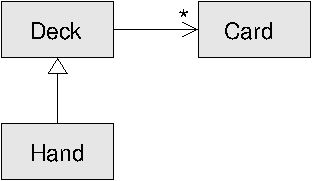
\includegraphics[scale=0.8]{figs/class1.pdf}}
\caption{Class diagram.}
\label{fig.class1}
\end{figure}


The arrow with a hollow triangle head represents an IS-A
relationship; in this case it indicates that Hand inherits
from Deck.

The standard arrow head represents a HAS-A
relationship; in this case a Deck has references to Card
objects.
\index{multiplicity (in class diagram)}

The star ({\tt *}) near the arrow head is a
{\bf multiplicity}; it indicates how many Cards a Deck has.
A multiplicity can be a simple number, like {\tt 52}, a range,
like {\tt 5..7} or a star, which indicates that a Deck can
have any number of Cards.

A more detailed diagram might show that a Deck actually
contains a {\em list} of Cards, but built-in types
like list and dict are usually not included in class diagrams.

\begin{exercise}

Read {\tt TurtleWorld.py}, {\tt World.py} and {\tt Gui.py}
and draw a class diagram that shows the relationships among
the classes defined there.

\end{exercise}


\section{Debugging}
\index{debugging}

Inheritance can make debugging a challenge because when you
invoke a method on an object, you might not know which method
will be invoked.
\index{polymorphism}

Suppose you are writing a function that works with Hand objects.
You would like it to work with all kinds of Hands, like
PokerHands, BridgeHands, etc.  If you invoke a method like
{\tt shuffle}, you might get the one defined in {\tt Deck},
but if any of the subclasses override this method, you'll
get that version instead.
\index{flow of execution}

Any time you are unsure about the flow of execution through your
program, the simplest solution is to add print statements at the
beginning of the relevant methods.  If {\tt Deck.shuffle} prints a
message that says something like {\tt Running Deck.shuffle}, then as
the program runs it traces the flow of execution.

As an alternative, you could use this function, which takes an
object and a method name (as a string) and returns the class that
provides the definition of the method:

\begin{verbatim}
def find_defining_class(obj, meth_name):
    for ty in type(obj).mro():
        if meth_name in ty.__dict__:
            return ty
\end{verbatim}
%
Here's an example:

\begin{verbatim}
>>> hand = Hand()
>>> print find_defining_class(hand, 'shuffle')
<class 'Card.Deck'>
\end{verbatim}
%
So the {\tt shuffle} method for this Hand is the one in {\tt Deck}.
\index{mro method}
\index{method!mro}
\index{method resolution order}

\verb"find_defining_class" uses the {\tt mro} method to get the list
of class objects (types) that will be searched for methods.  ``MRO''
stands for ``method resolution order.''
\index{override}
\index{interface}
\index{precondition}
\index{postcondition}

Here's a program design suggestion: whenever you override a method,
the interface of the new method should be the same as the old.  It
should take the same parameters, return the same type, and obey the
same preconditions and postconditions.  If you obey this rule, you
will find that any function designed to work with an instance of a
superclass, like a Deck, will also work with instances of subclasses
like a Hand or PokerHand.

If you violate this rule, your code will collapse like (sorry)
a house of cards.


\section{Data encapsulation}

Chapter~\ref{time} demonstrates a development plan we might call
``object-oriented design.''  We identified objects we needed---{\tt
  Time}, {\tt Point} and {\tt Rectangle}---and defined classes to
represent them.  In each case there is an obvious correspondence
between the object and some entity in the real world (or at least a
mathematical world).
\index{development plan}

But sometimes it is less obvious what objects you need
and how they should interact.  In that case you need a different
development plan.  In the same way that we discovered function
interfaces by encapsulation and generalization, we can discover
class interfaces by {\bf data encapsulation}.
\index{data encapsulation}
\index{encapsulation!data}

Markov analysis, from Section~\ref{markov}, provides a good example.
If you download my code from \url{http://thinkpython.com/code/markov.py},
you'll see that it uses two global variables---\verb"suffix_map" and
\verb"prefix"---that are read and written from several functions.

\begin{verbatim}
suffix_map = {}
prefix = ()
\end{verbatim}

Because these variables are global
we can only run one analysis
at a time.  If we read two texts, their prefixes and suffixes would
be added to the same data structures (which makes for some interesting
generated text).

To run multiple analyses, and keep them separate, we can encapsulate
the state of each analysis in an object.
Here's what that looks like:

\begin{verbatim}
class Markov(object):

    def __init__(self):
        self.suffix_map = {}
        self.prefix = ()
\end{verbatim}

Next, we transform the functions into methods.  For example,
here's \verb"process_word":

\begin{verbatim}
    def process_word(self, word, order=2):
        if len(self.prefix) < order:
            self.prefix += (word,)
            return

        try:
            self.suffix_map[self.prefix].append(word)
        except KeyError:
            # if there is no entry for this prefix, make one
            self.suffix_map[self.prefix] = [word]

        self.prefix = shift(self.prefix, word)
\end{verbatim}

Transforming a program like this---changing the design without
changing the function---is another example of refactoring
(see Section~\ref{refactoring}).
\index{refactoring}

This example suggests a development plan for designing objects and
methods:

\begin{enumerate}

\item Start by writing functions that read and write global
variables (when necessary).

\item Once you get the program working, look for associations
between global variables and the functions that use them.

\item Encapsulate related variables as attributes of an object.

\item Transform the associated functions into methods of the new
class.

\end{enumerate}


\begin{exercise}

Download my code from Section~\ref{markov}
(\url{http://thinkpython.com/code/markov.py}), and follow the steps described
above to encapsulate the global variables as attributes of a new class
called {\tt Markov}.  Solution: \url{http://thinkpython.com/code/Markov.py}
(note the capital M).

\end{exercise}




\section{Glossary}

\begin{description}

\item[encode:]  To represent one set of values using another
set of values by constructing a mapping between them.
\index{encode}

\item[class attribute:] An attribute associated with a class
object.  Class attributes are defined inside
a class definition but outside any method.
\index{class attribute}
\index{attribute!class}

\item[instance attribute:] An attribute associated with an
instance of a class.
\index{instance attribute}
\index{attribute!instance}

\item[veneer:] A method or function that provides a different
interface to another function without doing much computation.
\index{veneer}

\item[inheritance:] The ability to define a new class that is a
modified version of a previously defined class.
\index{inheritance}

\item[parent class:] The class from which a child class inherits.
\index{parent class}

\item[child class:] A new class created by inheriting from an
existing class; also called a ``subclass.''
\index{child class}
\index{class!child}

\item[IS-A relationship:] The relationship between a child class
and its parent class.
\index{IS-A relationship}

\item[HAS-A relationship:] The relationship between two classes
where instances of one class contain references to instances of
the other.
\index{HAS-A relationship}

\item[class diagram:] A diagram that shows the classes in a program
and the relationships between them.
\index{class diagram}
\index{diagram!class}

\item[multiplicity:] A notation in a class diagram that shows, for
a HAS-A relationship, how many references there are to instances
of another class.
\index{multiplicity (in class diagram)}

\end{description}


\section{Exercises}

\begin{exercise}
\label{poker}

The following are the possible hands in poker, in increasing order
of value (and decreasing order of probability):
\index{poker}

\begin{description}

\item[pair:] two cards with the same rank
\vspace{-0.05in}

\item[two pair:] two pairs of cards with the same rank
\vspace{-0.05in}

\item[three of a kind:] three cards with the same rank
\vspace{-0.05in}

\item[straight:] five cards with ranks in sequence (aces can
be high or low, so {\tt Ace-2-3-4-5} is a straight and so is {\tt
10-Jack-Queen-King-Ace}, but {\tt Queen-King-Ace-2-3} is not.)
\vspace{-0.05in}

\item[flush:] five cards with the same suit
\vspace{-0.05in}

\item[full house:] three cards with one rank, two cards with another
\vspace{-0.05in}

\item[four of a kind:] four cards with the same rank
\vspace{-0.05in}

\item[straight flush:] five cards in sequence (as defined above) and
with the same suit
\vspace{-0.05in}

\end{description}
%
The goal of these exercises is to estimate
the probability of drawing these various hands.

\begin{enumerate}

\item Download the following files from \url{http://thinkpython.com/code}:

\begin{description}

\item[{\tt Card.py}]: A complete version of the {\tt Card},
{\tt Deck} and {\tt Hand} classes in this chapter.

\item[{\tt PokerHand.py}]: An incomplete implementation of a class
that represents a poker hand, and some code that tests it.

\end{description}
%
\item If you run {\tt PokerHand.py}, it deals seven 7-card poker hands
and checks to see if any of them contains a flush.  Read this
code carefully before you go on.

\item Add methods to {\tt PokerHand.py} named \verb"has_pair",
\verb"has_twopair", etc. that return True or False according to
whether or not the hand meets the relevant criteria.  Your code should
work correctly for ``hands'' that contain any number of cards
(although 5 and 7 are the most common sizes).

\item Write a method named {\tt classify} that figures out
the highest-value classification for a hand and sets the
{\tt label} attribute accordingly.  For example, a 7-card hand
might contain a flush and a pair; it should be labeled ``flush''.

\item When you are convinced that your classification methods are
working, the next step is to estimate the probabilities of the various
hands.  Write a function in {\tt PokerHand.py} that shuffles a deck of
cards, divides it into hands, classifies the hands, and counts the
number of times various classifications appear.

\item Print a table of the classifications and their probabilities.
Run your program with larger and larger numbers of hands until the
output values converge to a reasonable degree of accuracy.  Compare
your results to the values at \url{http://en.wikipedia.org/wiki/Hand_rankings}.

\end{enumerate}

Solution: \url{http://thinkpython.com/code/PokerHandSoln.py}.
\end{exercise}


\begin{exercise}
\index{Swampy}
\index{TurtleWorld}

This exercise uses TurtleWorld from Chapter~\ref{turtlechap}.
You will write code that makes Turtles play tag.  If you
are not familiar with the rules of tag, see
\url{http://en.wikipedia.org/wiki/Tag_(game)}.

\begin{enumerate}

\item Download \url{http://thinkpython.com/code/Wobbler.py} and run it.  You
should see a TurtleWorld with three Turtles.  If you press the
{\sf Run} button, the Turtles wander at random.

\item Read the code and make sure you understand how it works.
The {\tt Wobbler} class inherits from {\tt Turtle}, which means
that the {\tt Turtle} methods {\tt lt}, {\tt rt}, {\tt fd}
and {\tt bk} work on Wobblers.

The {\tt step} method gets invoked by TurtleWorld.  It invokes
{\tt steer}, which turns the Turtle in the desired direction,
{\tt wobble}, which makes a random turn in proportion to the Turtle's
clumsiness, and {\tt move}, which moves forward a few pixels,
depending on the Turtle's speed.
\index{Tagger}

\item Create a file named {\tt Tagger.py}.  Import everything from
  {\tt Wobbler}, then define a class named {\tt Tagger} that inherits
  from {\tt Wobbler}.  Call \verb"make_world" passing the {\tt
    Tagger} class object as an argument.

\item Add a {\tt steer} method to {\tt Tagger} to override the one in
  {\tt Wobbler}.  As a starting place, write a version that always
  points the Turtle toward the origin.  Hint: use the math function
  {\tt atan2} and the Turtle attributes {\tt x}, {\tt y} and
  {\tt heading}.

\item Modify {\tt steer} so that the Turtles stay in bounds.
  For debugging, you might want to use the {\sf Step} button,
  which invokes {\tt step} once on each Turtle.

\item Modify {\tt steer} so that each Turtle points toward its nearest
  neighbor.  Hint: Turtles have an attribute, {\tt world}, that is a
  reference to the TurtleWorld they live in, and the TurtleWorld has
  an attribute, {\tt animals}, that is a list of all Turtles in the
  world.

\item Modify {\tt steer} so the Turtles play tag.  You can add methods
  to {\tt Tagger} and you can override {\tt steer} and
  \verb"__init__", but you may not modify or override {\tt step}, {\tt
    wobble} or {\tt move}.  Also, {\tt steer} is allowed to change the
  heading of the Turtle but not the position.

Adjust the rules and your {\tt steer} method for good quality play;
for example, it should be possible for the slow Turtle to tag the
faster Turtles eventually.

\end{enumerate}

Solution: \url{http://thinkpython.com/code/Tagger.py}.
\end{exercise}



\chapter{Case study: Tkinter}
\label{tkinter}

\section{GUI}

Most of the programs we have seen so far are text-based, but
many programs use {\bf graphical user interfaces}, also
known as {\bf GUIs}.
\index{GUI}
\index{graphical user interface}
\index{Tkinter}

Python provides several choices for writing GUI-based programs,
including wxPython, Tkinter, and Qt.  Each has pros and cons, which
is why Python has not converged on a standard.

The one I will present in this chapter is Tkinter because I think
it is the easiest to get started with.  Most of the concepts
in this chapter apply to the other GUI modules, too.

There are several books and web pages about Tkinter.  One of
the best online resources is {\em An Introduction to Tkinter}
by Fredrik Lundh.
\index{Gui module}
\index{module!Gui}
\index{Swampy}

I have written a module called {\tt Gui.py} that comes with
Swampy.  It provides a simplified interface to the functions
and classes in Tkinter.  The examples in this chapter are
based on this module.

Here is a simple example that creates and displays a Gui:

To create a GUI, you have to import {\tt Gui} from Swampy:
%
\begin{verbatim}
from swampy.Gui import *
\end{verbatim}
%
Or, depending on how you installed Swampy, like this:
%
\begin{verbatim}
from Gui import *
\end{verbatim}
%
Then instantiate a Gui object:
%
\begin{verbatim}
g = Gui()
g.title('Gui')
g.mainloop()
\end{verbatim}
%
When you run this code, a window should appear with an empty gray
square and the title {\sf Gui}.  {\tt mainloop} runs the {\bf event
  loop}, which waits for the user to do something and responds
accordingly.  It is an infinite loop; it runs until the user closes
the window, or presses Control-C, or does something that causes the
program to quit.
\index{event loop}
\index{loop!event}
\index{infinite loop}
\index{loop!infinite}

This Gui doesn't do much because it doesn't have any
{\bf widgets}.  Widgets are the elements that make up a
GUI; they include:
\index{widget}

\begin{description}

\item[Button:] A widget, containing text or an image, that
performs an action when pressed.

\item[Canvas:] A region that can display lines, rectangles,
circles and other shapes.

\item[Entry:] A region where users can type text.

\item[Scrollbar:] A widget that controls the visible part of another
widget.

\item[Frame:] A container, often invisible, that contains other
widgets.

\end{description}

The empty gray square you see when you create a Gui is
a Frame.  When you create a new widget, it is added to this Frame.



\section{Buttons and callbacks}
\index{Button widget}
\index{widget!Button}

The method {\tt bu} creates a Button widget:

\begin{verbatim}
button = g.bu(text='Press me.')
\end{verbatim}
%
The return value from {\tt bu} is a Button object.  The button
that appears in the Frame is a graphical representation of this
object; you can control the button by invoking methods on it.
\index{option}

{\tt bu} takes up to 32 parameters that control the appearance
and function of the button.  These parameters are called
{\bf options}.  Instead of providing values for all 32 options,
you can use keyword arguments, like \verb"text='Press me.'",
to specify only the options you need and use the default
values for the rest.
\index{keyword argument}
\index{argument!keyword}

When you add a widget to the Frame, it gets ``shrink-wrapped;''
that is, the Frame shrinks to the size of the Button.  If you
add more widgets, the Frame grows to accommodate them.
\index{Label widget}
\index{widget!Label}

The method {\tt la} creates a Label widget:

\begin{verbatim}
label = g.la(text='Press the button.')
\end{verbatim}
%
By default, Tkinter stacks the widgets top-to-bottom and centers
them.  We'll see how to override that behavior soon.

If you press the button, you will see that it doesn't do much.
That's because you haven't ``wired it up;'' that is, you haven't
told it what to do!

The option that controls the behavior of a button is {\tt command}.
The value of {\tt command} is a function that gets executed when
the button is pressed.  For example, here is a function that creates
a new Label:

\begin{verbatim}
def make_label():
    g.la(text='Thank you.')
\end{verbatim}
%
Now we can create a button with this function as its command:

\begin{verbatim}
button2 = g.bu(text='No, press me!', command=make_label)
\end{verbatim}
%
When you press this button, it should execute \verb"make_label"
and a new label should appear.
\index{callback}

The value of the {\tt command} option
is a function object, which is known as a {\bf callback} because
after you call {\tt bu} to create the button, the flow of execution
``calls back'' when the user presses the button.
\index{event-driven programming}

This kind of flow is characteristic of {\bf event-driven programming}.
User actions, like button presses and key strokes, are called {\bf
events}.  In event-driven programming, the flow of execution is
determined by user actions rather than by the programmer.

The challenge of event-driven programming is to construct a set of
widgets and callbacks that work correctly (or at least generate
appropriate error messages) for any sequence of user actions.

\begin{exercise}

Write a program that creates a GUI with a single button.  When the
button is pressed it should create a second button.  When
{\em that} button is pressed, it should create a label that
says, ``Nice job!''.

What happens if you press the buttons more than once?
Solution: \url{http://thinkpython.com/code/button_demo.py}

\end{exercise}


\section{Canvas widgets}
\index{Canvas widget}
\index{widget!Canvas}

One of the most versatile widgets is the Canvas, which creates
a region for drawing lines, circles and other shapes.  If you
did Exercise~\ref{canvas} you are already familiar with canvases.

The method {\tt ca} creates a new Canvas:

\begin{verbatim}
canvas = g.ca(width=500, height=500)
\end{verbatim}
%
{\tt width} and {\tt height} are the dimensions of the canvas
in pixels.
\index{config method}
\index{method!config}

After you create a widget, you can still change the values of
the options with the
{\tt config} method.  For example, the {\tt bg} option changes
the background color:

\begin{verbatim}
canvas.config(bg='white')
\end{verbatim}
%
The value of {\tt bg} is a string
that names a color.  The set of legal color names is different
for different implementations of Python, but all implementations
provide at least:

\begin{verbatim}
white   black
red     green    blue
cyan    yellow   magenta
\end{verbatim}
%
Shapes on a Canvas are called {\bf items}.  For example,
the Canvas method {\tt circle} draws (you guessed it) a circle:
\index{Canvas item}
\index{item!Canvas}

\begin{verbatim}
item = canvas.circle([0,0], 100, fill='red')
\end{verbatim}
%
The first argument is a coordinate pair that specifies the
center of the circle; the second is the radius.
\index{Canvas coordinate}
\index{coordinate!Canvas}

{\tt Gui.py} provides a standard Cartesian coordinate system with
the origin at the center of the Canvas and the positive $y$ axis
pointing up.  This is different from some other graphics systems
where the origin is in the upper left corner, with the $y$ axis
pointing down.

The {\tt fill} option specifies that the circle should be filled
in with red.

The return value from {\tt circle} is an Item object that
provides methods for modifying the item on the canvas.  For
example, you can use {\tt config} to change any of the circle's
options:

\begin{verbatim}
item.config(fill='yellow', outline='orange', width=10)
\end{verbatim}
%
{\tt width} is the thickness of the outline in pixels;
{\tt outline} is the color.

\begin{exercise}
\label{circle}

Write a program that creates a Canvas and a Button.  When the
user presses the Button, it should draw a circle on the canvas.

\end{exercise}


\section{Coordinate sequences}
\index{coordinate sequence}
\index{sequence!coordinate}

The {\tt rectangle} method takes a sequence of coordinates that
specify opposite corners of the rectangle.  This example
draws a green rectangle with the lower left corner at the origin
and the upper right corner at $(200,100)$:

\begin{verbatim}
canvas.rectangle([[0, 0], [200, 100]],
                 fill='blue', outline='orange', width=10)
\end{verbatim}
%
This way of specifying corners is called
a {\bf bounding box} because the two points
bound the rectangle.
\index{bounding box}

{\tt oval} takes a bounding box and draws an oval
within the specified rectangle:

\begin{verbatim}
canvas.oval([[0, 0], [200, 100]], outline='orange', width=10)
\end{verbatim}
%
{\tt line} takes a sequence of coordinates and draws
a line that connects the points.  This example draws two legs
of a triangle:

\begin{verbatim}
canvas.line([[0, 100], [100, 200], [200, 100]], width=10)
\end{verbatim}
%
{\tt polygon} takes the same arguments, but it draws the last
leg of the polygon (if necessary) and fills it in:

\begin{verbatim}
canvas.polygon([[0, 100], [100, 200], [200, 100]],
               fill='red', outline='orange', width=10)
\end{verbatim}
%


\section{More widgets}
\index{Text widget}
\index{widget!Text}

Tkinter provides two widgets that let users type text: an
Entry, which is a single line, and a Text widget, which has
multiple lines.
\index{Entry widget}
\index{widget!Entry}

{\tt en} creates a new Entry:

\begin{verbatim}
entry = g.en(text='Default text.')
\end{verbatim}
%
The {\tt text} option allows you to put text into the entry
when it is created.  The {\tt get} method returns the contents
of the Entry (which may have been changed by the user):

\begin{verbatim}
>>> entry.get()
'Default text.'
\end{verbatim}
%
{\tt te} creates a Text widget:

\begin{verbatim}
text = g.te(width=100, height=5)
\end{verbatim}
%
{\tt width} and {\tt height} are the dimensions of the
widget in characters and lines.

{\tt insert} puts text into the Text widget:

\begin{verbatim}
text.insert(END, 'A line of text.')
\end{verbatim}
%
{\tt END} is a special index that indicates the last character in the
Text widget.

You can also specify a character using a dotted index, like {\tt 1.1},
which has the line number before the dot and the column number after.
The following example adds the letters \verb"'nother'" after the first
character of the first line.

\begin{verbatim}
>>> text.insert(1.1, 'nother')
\end{verbatim}
%
The {\tt get} method reads the text in the widget; it takes a start
and end index as arguments.  The following example returns all the
text in the widget, including the newline character:

\begin{verbatim}
>>> text.get(0.0, END)
'Another line of text.\n'
\end{verbatim}
%
The {\tt delete} method removes text from the widget;
the following example deletes all but the first two characters:

\begin{verbatim}
>>> text.delete(1.2, END)
>>> text.get(0.0, END)
'An\n'
\end{verbatim}
%

\begin{exercise}
\label{circle2}

Modify your solution to Exercise~\ref{circle} by adding an
Entry widget and a second button.  When the user presses the
second button, it should read a color name from the Entry and
use it to change the fill color of the circle.  Use {\tt config}
to modify the existing circle; don't create a new one.

Your program should handle the case where the user tries to
change the color of a circle that hasn't been created, and
the case where the color name is invalid.

You can see my solution at \url{http://thinkpython.com/code/circle_demo.py}.

\end{exercise}


\section{Packing widgets}

So far we have been stacking widgets in a single column, but in most
GUIs the layout is more complicated.  For example,
Figure~\ref{fig.turtleworld} shows a simplified version of
TurtleWorld (see Chapter~\ref{turtlechap}).

\begin{figure}
\centerline{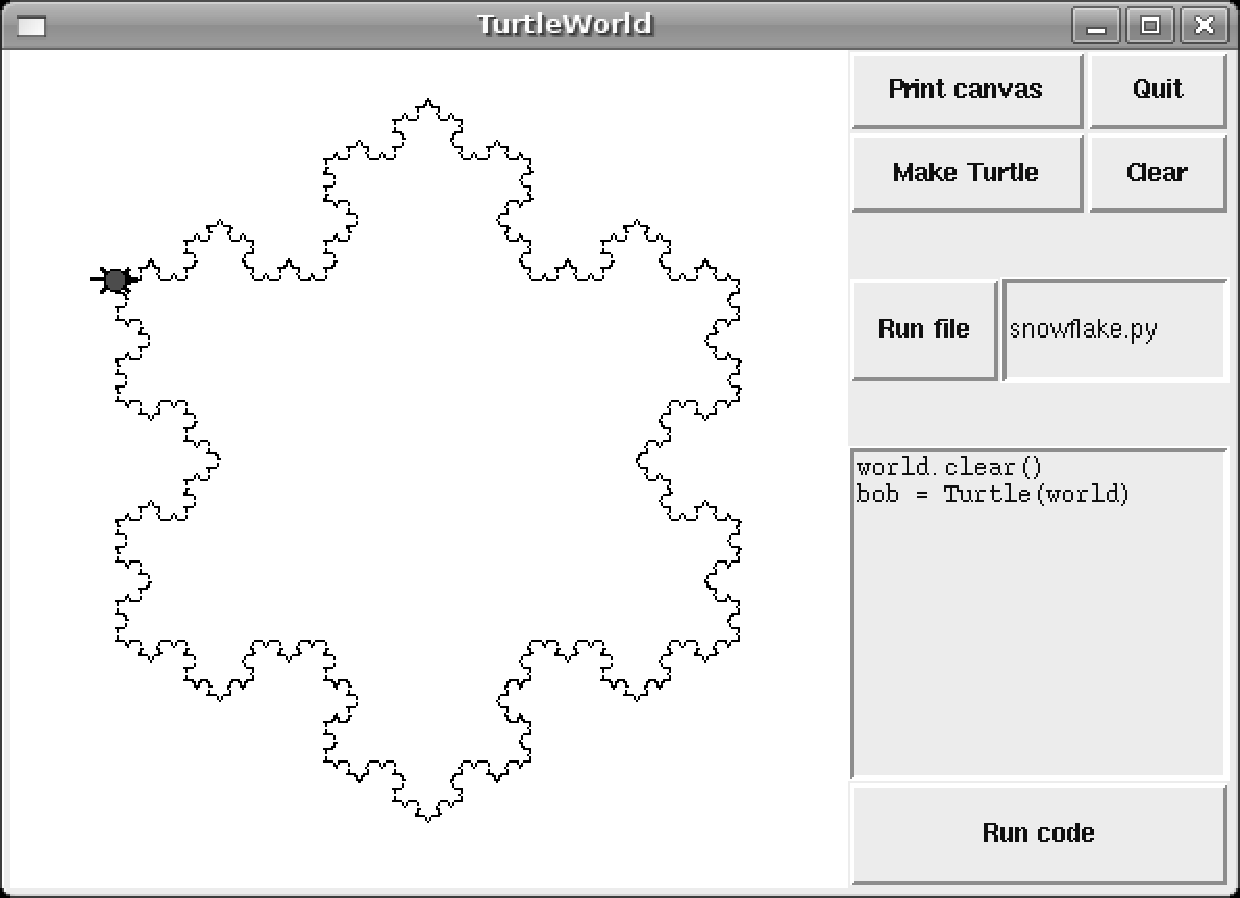
\includegraphics[scale=0.5]{figs/TurtleWorld.pdf}}
\caption{Class diagram.}
\label{fig.turtleworld}
\end{figure}


This section presents the code that creates this GUI, broken into a
series of steps.  You can download the complete example
from \url{http://thinkpython.com/code/SimpleTurtleWorld.py}.

At the top level, this GUI contains two widgets---a Canvas and a
Frame---arranged in a row.  So the first step is to create the row.
\index{SimpleTurtleWorld class}
\index{class!SimpleTurtleWorld}

\begin{verbatim}
class SimpleTurtleWorld(TurtleWorld):
    """This class is identical to TurtleWorld, but the code that
    lays out the GUI is simplified for explanatory purposes."""

    def setup(self):
        self.row()
        ...
\end{verbatim}
%
{\tt setup} is the function that creates and arranges the widgets.
Arranging widgets in a GUI is called {\bf packing}.
\index{packing widgets}
\index{widget, packing}
\index{Frame widget}
\index{widget!Frame}

{\tt row} creates a row Frame and makes it the ``current Frame.''
Until this Frame is closed or another Frame is created, all
subsequent widgets are packed in a row.

Here is the code that creates the Canvas and the column Frame
that hold the other widgets:

\begin{verbatim}
        self.canvas = self.ca(width=400, height=400, bg='white')
        self.col()
\end{verbatim}
%
The first widget in the column is a grid Frame, which contains
four buttons arranged two-by-two:

\begin{verbatim}
        self.gr(cols=2)
        self.bu(text='Print canvas', command=self.canvas.dump)
        self.bu(text='Quit', command=self.quit)
        self.bu(text='Make Turtle', command=self.make_turtle)
        self.bu(text='Clear', command=self.clear)
        self.endgr()
\end{verbatim}
%
{\tt gr} creates the grid; the argument is the number of
columns.  Widgets in the grid are
laid out left-to-right, top-to-bottom.
\index{callback}
\index{bound method}
\index{method, bound}
\index{subject}

The first button uses {\tt self.canvas.dump} as a callback; the second
uses {\tt self.quit}.  These are {\bf bound methods}, which means they
are associated with a particular object.  When they are invoked, they
are invoked on the object.

The next widget in the column is a row Frame that contains
a Button and an Entry:

\begin{verbatim}
        self.row([0,1], pady=30)
        self.bu(text='Run file', command=self.run_file)
        self.en_file = self.en(text='snowflake.py', width=5)
        self.endrow()
\end{verbatim}
%
The first argument to {\tt row} is a list of weights that
determines how extra space is allocated between widgets.
The list {\tt [0,1]} means that all extra space is allocated
to the second widget, which is the Entry.  If you run this code
and resize the window, you will see that the Entry grows and
the Button doesn't.

The option {\tt pady} ``pads'' this row in the $y$ direction,
adding 30 pixels of space above and below.

{\tt endrow} ends this row of widgets, so subsequent widgets are
packed in the column Frame.  {\tt Gui.py} keeps a stack of Frames:

\begin{itemize}

\item When you use {\tt row}, {\tt col} or {\tt gr} to create a Frame,
it goes on top of the stack and becomes the current Frame.

\item When you use {\tt endrow}, {\tt endcol} or {\tt endgr} to close
a Frame, it gets popped off the stack and the previous Frame on the
stack becomes the current Frame.

\end{itemize}

The method \verb"run_file" reads the contents of the Entry,
uses it as a filename, reads the contents
and passes it to \verb"run_code".  {\tt self.inter} is an
Interpreter object that knows how to take a string and
execute it as Python code.

\begin{verbatim}
    def run_file(self):
        filename = self.en_file.get()
        fp = open(filename)
        source = fp.read()
        self.inter.run_code(source, filename)
\end{verbatim}
%
The last two widgets are a Text widget and a Button:

\begin{verbatim}
        self.te_code = self.te(width=25, height=10)
        self.te_code.insert(END, 'world.clear()\n')
        self.te_code.insert(END, 'bob = Turtle(world)\n')

        self.bu(text='Run code', command=self.run_text)
\end{verbatim}
%
\verb"run_text" is similar to \verb"run_file" except that it takes
the code from the Text widget instead of from a file:

\begin{verbatim}
    def run_text(self):
        source = self.te_code.get(1.0, END)
        self.inter.run_code(source, '<user-provided code>')
\end{verbatim}
%
Unfortunately, the details of widget layout are different in
other languages, and in different Python modules.
Tkinter alone provides three different mechanisms for arranging
widgets.  These mechanisms are called {\bf geometry managers}.
The one I demonstrated in this section is the ``grid'' geometry
manager; the others are called ``pack'' and ``place''.
\index{geometry manager}

Fortunately, most of the concepts in this section apply to
other GUI modules and other languages.


\section{Menus and Callables}
\index{Menubutton widget}
\index{widget!Menubutton}

A Menubutton is a widget that looks like a button, but when pressed
it pops up a menu.  After the user selects an item, the menu
disappears.

Here is code that creates a color selection Menubutton
(you can download it from \url{http://thinkpython.com/code/menubutton_demo.py}):

\begin{verbatim}
g = Gui()
g.la('Select a color:')
colors = ['red', 'green', 'blue']
mb = g.mb(text=colors[0])
\end{verbatim}
%
{\tt mb} creates the Menubutton.  Initially, the text on the button is
the name of the default color.  The following loop creates one menu
item for each color:

\begin{verbatim}
for color in colors:
    g.mi(mb, text=color, command=Callable(set_color, color))
\end{verbatim}
%
The first argument of {\tt mi} is the Menubutton these items are
associated with.
\index{callback}
\index{Callable object}
\index{object!Callable}

The {\tt command} option is a Callable object, which is something new.
So far we have seen functions and bound methods used as callbacks,
which works fine if you don't have to pass any arguments to
the function.  Otherwise you have to construct a Callable object
that contains a function, like \verb"set_color", and its arguments,
like {\tt color}.

The Callable object stores a reference to the function and the
arguments as attributes.  Later, when the user clicks on a menu
item, the callback calls the function and passes the stored
arguments.

Here is what \verb"set_color" might look like:

\begin{verbatim}
def set_color(color):
    mb.config(text=color)
    print color
\end{verbatim}
%
When the user selects a menu item and \verb"set_color" is called,
it configures the Menubutton to display the newly-selected color.
It also print the color; if you try this example, you can confirm that
\verb"set_color" is called when you select an item (and {\em not}
called when you create the Callable object).


\section{Binding}
\index{binding}
\index{callback}

A {\bf binding} is an association between a widget, an event and a
callback: when an event (like a button press) happens on a widget, the
callback is invoked.

Many widgets have default bindings.  For example, when you press
a button, the default binding changes the relief of the button
to make it look depressed.  When you release the button, the
binding restores the appearance of the button and invokes the
callback specified with the {\tt command} option.

You can use the {\tt bind} method to override these default
bindings or to add new ones.  For example, this code creates a
binding for a canvas (you can download the code in this
section from \url{http://thinkpython.com/code/draggable_demo.py}):

\begin{verbatim}
ca.bind('<ButtonPress-1>', make_circle)
\end{verbatim}
%
The first argument is an event string; this event is triggered
when the user presses the left mouse button.  Other mouse
events include {\tt ButtonMotion}, {\tt ButtonRelease} and
{\tt Double-Button}.
\index{event string}
\index{event handler}

The second argument is an event handler.  An event handler
is a function or bound method, like a callback, but an important
difference is that an event handler takes an Event object as a
parameter.  Here is an example:

\begin{verbatim}
def make_circle(event):
    pos = ca.canvas_coords([event.x, event.y])
    item = ca.circle(pos, 5, fill='red')
\end{verbatim}
%
The Event object contains information about the type of event and
details like the coordinates of the mouse pointer.  In this example
the information we need is
the location of the mouse click.  These
values are in ``pixel coordinates,'' which are defined by the
underlying graphical system.  The method \verb"canvas_coords"
translates them to ``Canvas coordinates,'' which are compatible with
Canvas methods like {\tt circle}.
\index{Event object}
\index{object!Event}

For Entry widgets, it is common to bind the \verb"<Return>" event,
which is triggered when the user presses the {\sf Return} or
{\sf Enter} key.  For example, the following code creates a Button
and an Entry.

\begin{verbatim}
bu = g.bu('Make text item:', make_text)
en = g.en()
en.bind('<Return>', make_text)
\end{verbatim}
%
\verb"make_text" is called when the Button is pressed or when
the user hits {\sf Return} while typing in the Entry.  To make
this work, we need a function that can be called as a command
(with no arguments) or as an event handler (with an Event
as an argument):

\begin{verbatim}
def make_text(event=None):
    text = en.get()
    item = ca.text([0,0], text)
\end{verbatim}
%
\verb"make_text" gets the contents of the Entry and displays
it as a Text item in the Canvas.

It is also possible to create bindings for Canvas items.
The following is a class definition for {\tt Draggable},
which is a child class of {\tt Item} that provides bindings
that implement drag-and-drop capability.
\index{drag-and-drop}

\begin{verbatim}
class Draggable(Item):

    def __init__(self, item):
        self.canvas = item.canvas
        self.tag = item.tag
        self.bind('<Button-3>', self.select)
        self.bind('<B3-Motion>', self.drag)
        self.bind('<Release-3>', self.drop)
\end{verbatim}
%
The init method takes an Item as a parameter.  It copies
the attributes of the Item and then creates bindings for
three events: a button press, button motion, and button release.

The event handler {\tt select} stores the coordinates
of the current event and the original color of the item, then
changes the color to yellow:

\begin{verbatim}
    def select(self, event):
        self.dragx = event.x
        self.dragy = event.y

        self.fill = self.cget('fill')
        self.config(fill='yellow')
\end{verbatim}
%
{\tt cget} stands for ``get configuration;'' it takes the name of an
option as a string and returns the current value of that option.

{\tt drag} computes how far the object has moved relative to the
starting place, updates the stored coordinates, and then moves the
item.
\index{update!coordinate}

\begin{verbatim}
    def drag(self, event):
        dx = event.x - self.dragx
        dy = event.y - self.dragy

        self.dragx = event.x
        self.dragy = event.y

        self.move(dx, dy)
\end{verbatim}
%
This computation is done in pixel coordinates; there is no need to
convert to Canvas coordinates.
\index{Canvas coordinate}
\index{coordinate!Canvas}
\index{pixel coordinate}
\index{coordinate!pixel}

Finally, {\tt drop} restores the original color of the item:

\begin{verbatim}
    def drop(self, event):
        self.config(fill=self.fill)
\end{verbatim}
%
You can use the {\tt Draggable} class to add drag-and-drop
capability to an existing item.  For example, here is a modified
version of \verb"make_circle" that uses {\tt circle} to create
an Item and {\tt Draggable} to make it draggable:

\begin{verbatim}
def make_circle(event):
    pos = ca.canvas_coords([event.x, event.y])
    item = ca.circle(pos, 5, fill='red')
    item = Draggable(item)
\end{verbatim}
%
This example demonstrates one of the benefits of inheritance: you can
modify the capabilities of a parent class without modifying its
definition.  This is particularly useful if you want to change
behavior defined in a module you did not write.


\section{Debugging}
\index{debugging}

One of the challenges of GUI programming is keeping track of
which things happen while the GUI is being built and which
things happen later in response to user events.
\index{callback}

For example, when you are setting up a callback, it is a common error
to call the function rather than passing a reference to it:

\begin{verbatim}
def the_callback():
    print 'Called.'

g.bu(text='This is wrong!', command=the_callback())
\end{verbatim}
%
If you run this code, you will see that it calls \verb"the_callback"
immediately, and {\em then} creates the button.  When you press the
button, it does nothing because the return value from
\verb"the_callback" is {\tt None}.
Usually you do not want to invoke a callback while you are
setting up the GUI; it should only be invoked later in response to
a user event.
\index{flow of execution}
\index{event-driven programming}

Another challenge of GUI programming is that you don't have control
of the flow of execution.  Which parts of the program execute
and their order are determined by user actions.
That means that you have to design your program to work correctly
for any possible sequence of events.

For example, the GUI in Exercise~\ref{circle2} has two widgets:
one creates a Circle item and the other changes the color of the
Circle.  If the user creates the circle and then changes its color,
there's no problem.  But what if the user changes the color of
a circle that doesn't exist yet?  Or creates more than one circle?

As the number of widgets grows, it is increasingly difficult to
imagine all possible sequences of events.  One way to manage this
complexity is to encapsulate the state of the system in an object
and then consider:

\begin{itemize}

\item What are the possible states?  In the Circle example, we
might consider two states: before and after the user creates the
first circle.

\item In each state, what events can occur?  In the example,
the user can press either of the buttons, or quit.

\item For each state-event pair, what is the desired outcome?
Since there are two states and two buttons, there are four
state-event pairs to consider.

\item What can cause a transition from one state to another?
In this case, there is a transition when the user creates
the first circle.

\end{itemize}

You might also find it useful to define, and check, invariants that
should hold regardless of the sequence of events.
\index{invariant}

This approach to GUI programming can help you write correct
code without taking the time to test every possible sequence
of user events!


\section{Glossary}

\begin{description}

\item[GUI:] A graphical user interface.
\index{GUI}

\item[widget:] One of the elements that makes up a GUI, including
buttons, menus, text entry fields, etc.
\index{widget}

\item[option:] A value that controls the appearance or function of
a widget.
\index{option}

\item[keyword argument:] An argument that indicates the parameter
name as part of the function call.
\index{keyword argument}

\item[callback:] A function associated with a widget that is
called when the user performs an action.
\index{callback}

\item[bound method:] A method associated with a particular instance.
\index{bound method}

\item[event-driven programming:] A style of programming in which
the flow of execution is determined by user actions.
\index{event-driven programming}

\item[event:] A user action, like a mouse click or key press, that
causes a GUI to respond.
\index{event}

\item[event loop:] An infinite loop that waits for user actions
and responds.
\index{event loop}

\item[item:] A graphical element on a Canvas widget.
\index{item!Canvas}

\item[bounding box:] A rectangle that encloses a set of items,
usually specified by two opposing corners.
\index{bounding box}

\item[pack:] To arrange and display the elements of a GUI.
\index{packing widgets}

\item[geometry manager:] A system for packing widgets.
\index{geometry manager}

\item[binding:] An association between a widget, an event, and
an event handler.  The event handler is called when the event
occurs in the widget.
\index{binding}

\end{description}


\section{Exercises}

\begin{exercise}
\index{image viewer}

For this exercise, you will write an image viewer.  Here is
a simple example:

\begin{verbatim}
g = Gui()
canvas = g.ca(width=300)
photo = PhotoImage(file='danger.gif')
canvas.image([0,0], image=photo)
g.mainloop()
\end{verbatim}
%
{\tt PhotoImage} reads a file and returns a {\tt PhotoImage} object
that Tkinter can display.  {\tt Canvas.image} puts the image on the
canvas, centered on the given coordinates.  You can also put images on
labels, buttons, and some other widgets:

\begin{verbatim}
g.la(image=photo)
g.bu(image=photo)
\end{verbatim}
%
PhotoImage can only handle a few image formats, like GIF and PPM,
but we can use the Python Imaging Library (PIL) to read other
files.
\index{Python Imaging Library (PIL)}
\index{PIL (Python Imaging Library)}
\index{Image module}
\index{module!Image}

The name of the PIL module is {\tt Image}, but Tkinter defines an
object with the same name.  To avoid the conflict, you can use {\tt
  import...as} like this:

\begin{verbatim}
import Image as PIL
import ImageTk
\end{verbatim}
%
The first line imports {\tt Image} and
gives it the local name {\tt PIL}.  The second
line imports {\tt ImageTk}, which can translate a PIL
image into a Tkinter PhotoImage.  Here's an example:

\begin{verbatim}
image = PIL.open('allen.png')
photo2 = ImageTk.PhotoImage(image)
g.la(image=photo2)
\end{verbatim}
%

\begin{enumerate}

\item Download \verb"image_demo.py", \verb"danger.gif" and \verb"allen.png"
from \url{http://thinkpython.com/code}.  Run \verb"image_demo.py".  You
might have to install {\tt PIL} and {\tt ImageTk}.
They are probably in your software repository,  but if not
you can get them from \url{pythonware.com/products/pil/}.

\item In \verb"image_demo.py" change the name of the second
PhotoImage from {\tt photo2} to {\tt photo} and run the program
again.  You should see the second PhotoImage but not the first.

The problem is that when you reassign {\tt photo} it overwrites
the reference to the first PhotoImage, which then disappears.  The
same thing happens if you assign a PhotoImage to a local
variable; it disappears when the function ends.

To avoid this problem, you have to store a reference to each
PhotoImage you want to keep.  You can use a global variable, or
store PhotoImages in a data structure or as an attribute of
an object.

This behavior can be frustrating, which is why I am warning
you (and why the example image says ``Danger!'').
\index{bug!worst ever}
\index{worst bug!ever}

\item Starting with this example, write a program that takes
the name of a directory and loops through all the files, displaying
any files that PIL recognizes as images.  You can use a {\tt try}
statement to catch the files PIL doesn't recognize.

When the user clicks on the image, the program should display the next one.

\item PIL provides a variety of methods for manipulating images.
You can read about them at \url{http://pythonware.com/library/pil/handbook}.
As a challenge, choose a few of these methods and provide a
GUI for applying them to images.

\end{enumerate}

Solution: \url{http://thinkpython.com/code/ImageBrowser.py}.

\end{exercise}


\begin{exercise}
\index{vector graphics}
\index{SVG}

A vector graphics editor is a program that allows users to draw and
edit shapes on the screen and generate output files in vector graphics
formats like Postscript and SVG.

Write a simple vector graphics editor using Tkinter.  At a
minimum, it should allow users to draw lines, circles and
rectangles, and it should use {\tt Canvas.dump} to
generate a Postscript description of the contents of the
Canvas.

As a challenge, you could allow users to select and resize
items on the Canvas.

% TODO: write a solution!

\end{exercise}


\begin{exercise}

Use Tkinter to write a basic web browser.  It
should have a Text widget where the user can enter a URL
and a Canvas to display the contents of the page.
\index{urllib module}
\index{module!urllib}
\index{URL}
\index{HTMLParser module}
\index{module!HTMLParser}

You can use the {\tt urllib} module to download files
(see Exercise~\ref{urllib}) and
the {\tt HTMLParser} module to parse the HTML
tags (see \url{http://docs.python.org/2/library/htmlparser.html}).
\index{plain text}
\index{text!plain}
\index{hyperlink}

At a minimum your browser should handle plain text and hyperlinks.  As
a challenge you could handle background colors, text
formatting tags and images.

% TODO: write a solution!

\end{exercise}



\appendix

\chapter{Debugging}

\index{debugging}
Different kinds of errors can occur
in a program, and it is useful to distinguish among them
in order to track them down more quickly:

\begin{itemize}

\item Syntax errors are produced by Python when it is translating the
  source code into byte code.  They usually indicate that there is
  something wrong with the syntax of the program.  Example: Omitting
  the colon at the end of a {\tt def} statement yields the somewhat
  redundant message {\tt SyntaxError: invalid syntax}.

\item Runtime errors are produced by the interpreter if something goes
  wrong while the program is running.  Most runtime error messages
  include information about where the error occurred and what
  functions were executing.  Example: An infinite recursion eventually
  causes the runtime error ``maximum recursion depth exceeded.''

\item Semantic errors are problems with a program that runs without
  producing error messages but doesn't do the right thing.  Example:
  An expression may not be evaluated in the order you expect, yielding
  an incorrect result.

\end{itemize}
\index{syntax error}
\index{runtime error}
\index{semantic error}
\index{error!compile-time}
\index{error!syntax}
\index{error!runtime}
\index{error!semantic}
\index{exception}

The first step in debugging is to figure out which kind of
error you are dealing with.  Although the following sections are
organized by error type, some techniques are
applicable in more than one situation.


\section{Syntax errors}
\index{error message}

Syntax errors are usually easy to fix once you figure out what they
are.  Unfortunately, the error messages are often not helpful.
The most common messages are {\tt SyntaxError: invalid syntax} and
{\tt SyntaxError: invalid token}, neither of which is very informative.

On the other hand, the message does tell you where in the program the
problem occurred.  Actually, it tells you where Python
noticed a problem, which is not necessarily where the error
is.  Sometimes the error is prior to the location of the error
message, often on the preceding line.
\index{incremental development}
\index{development plan!incremental}

If you are building the program incrementally, you should have
a good idea about where the error is.  It will be in the last
line you added.

If you are copying code from a book, start by comparing
your code to the book's code very carefully.  Check every character.
At the same time, remember that the book might be wrong, so
if you see something that looks like a syntax error, it might be.

Here are some ways to avoid the most common syntax errors:
\index{syntax}

\begin{enumerate}

\item Make sure you are not using a Python keyword for a variable name.
\index{keyword}

\item Check that you have a colon at the end of the header of every
compound statement, including {\tt for}, {\tt while},
{\tt if}, and {\tt def} statements.
\index{header}
\index{colon}

\item Make sure that any strings in the code have matching
quotation marks.
\index{quotation mark}

\item If you have multiline strings with triple quotes (single or double), make
sure you have terminated the string properly.  An unterminated string
may cause an {\tt invalid token} error at the end of your program,
or it may treat the following part of the program as a string until it
comes to the next string.  In the second case, it might not produce an error
message at all!
\index{multiline string}
\index{string!multiline}

\item An unclosed opening operator---\verb+(+, \verb+{+, or
  \verb+[+---makes Python continue with the next line as part of the
  current statement.  Generally, an error occurs almost immediately in
  the next line.

\item Check for the classic {\tt =} instead of {\tt ==} inside
a conditional.
\index{conditional}

\item Check the indentation to make sure it lines up the way it
is supposed to.  Python can handle space and tabs, but if you mix
them it can cause problems.  The best way to avoid this problem
is to use a text editor that knows about Python and generates
consistent indentation.
\index{indentation}
\index{whitespace}

\end{enumerate}

If nothing works, move on to the next section...


\subsection{I keep making changes and it makes no difference.}

If the interpreter says there is an error and you don't see it, that
might be because you and the interpreter are not looking at the same
code.  Check your programming environment to make sure that the
program you are editing is the one Python is trying to run.

If you are not sure, try putting an obvious and deliberate syntax
error at the beginning of the program.  Now run it again.  If the
interpreter doesn't find the new error, you are not running the
new code.

There are a few likely culprits:

\begin{itemize}

\item You edited the file and forgot to save the changes before
running it again.  Some programming environments do this
for you, but some don't.

\item You changed the name of the file, but you are still running
the old name.

\item Something in your development environment is configured
incorrectly.

\item If you are writing a module and using {\tt import},
make sure you don't give your module the same name as one
of the standard Python modules.
\index{module!reload}
\index{reload function}
\index{function!reload}

\item If you are using {\tt import} to read a module, remember
that you have to restart the interpreter or use {\tt reload}
to read a modified file.  If you import the module again, it
doesn't do anything.

\end{itemize}

If you get stuck and you can't figure out what is going on, one
approach is to start again with a new program like ``Hello, World!,''
and make sure you can get a known program to run.  Then gradually add
the pieces of the original program to the new one.


\section{Runtime errors}

Once your program is syntactically correct,
Python can compile it and at least start running it.  What could
possibly go wrong?


\subsection{My program does absolutely nothing.}

This problem is most common when your file consists of functions and
classes but does not actually invoke anything to start execution.
This may be intentional if you only plan to import this module to
supply classes and functions.

If it is not intentional, make sure that you
are invoking a function to start execution, or execute one from
the interactive prompt.  Also see the ``Flow of Execution'' section
below.


\subsection{My program hangs.}
\index{infinite loop}
\index{infinite recursion}
\index{hanging}

If a program stops and seems to be doing nothing, it is ``hanging.''
Often that means that it is caught in an infinite loop or infinite
recursion.

\begin{itemize}

\item If there is a particular loop that you suspect is the
problem, add a {\tt print} statement immediately before the loop that says
``entering the loop'' and another immediately after that says
``exiting the loop.''

Run the program.  If you get the first message and not the second,
you've got an infinite loop.  Go to the ``Infinite Loop'' section
below.

\item Most of the time, an infinite recursion will cause the program
to run for a while and then produce a ``RuntimeError: Maximum
recursion depth exceeded'' error.  If that happens, go to the
``Infinite Recursion'' section below.

If you are not getting this error but you suspect there is a problem
with a recursive method or function, you can still use the techniques
in the ``Infinite Recursion'' section.

\item If neither of those steps works, start testing other
loops and other recursive functions and methods.

\item If that doesn't work, then it is possible that
you don't understand the flow of execution in your program.
Go to the ``Flow of Execution'' section below.

\end{itemize}


\subsubsection{Infinite Loop}
\index{infinite loop}
\index{loop!infinite}
\index{condition}
\index{loop!condition}

If you think you have an infinite loop and you think you know
what loop is causing the problem, add a {\tt print} statement at
the end of the loop that prints the values of the variables in
the condition and the value of the condition.

For example:

\begin{verbatim}
while x > 0 and y < 0 :
    # do something to x
    # do something to y

    print "x: ", x
    print "y: ", y
    print "condition: ", (x > 0 and y < 0)
\end{verbatim}
%
Now when you run the program, you will see three lines of output
for each time through the loop.  The last time through the
loop, the condition should be {\tt false}.  If the loop keeps
going, you will be able to see the values of {\tt x} and {\tt y},
and you might figure out why they are not being updated correctly.


\subsubsection{Infinite Recursion}
\index{infinite recursion}
\index{recursion!infinite}

Most of the time, an infinite recursion will cause the program to run
for a while and then produce a {\tt Maximum recursion depth exceeded}
error.

If you suspect that a function or method is causing an infinite
recursion, start by checking to make sure that there is a base case.
In other words, there should be some condition that will cause the
function or method to return without making a recursive invocation.
If not, then you need to rethink the algorithm and identify a base
case.

If there is a base case but the program doesn't seem to be reaching
it, add a {\tt print} statement at the beginning of the function or method
that prints the parameters.  Now when you run the program, you will see
a few lines of output every time the function or method is invoked,
and you will see the parameters.  If the parameters are not moving
toward the base case, you will get some ideas about why not.


\subsubsection{Flow of Execution}
\index{flow of execution}

If you are not sure how the flow of execution is moving through
your program, add {\tt print} statements to the beginning of each
function with a message like ``entering function {\tt foo},'' where
{\tt foo} is the name of the function.

Now when you run the program, it will print a trace of each
function as it is invoked.


\subsection{When I run the program I get an exception.}
\index{exception}
\index{runtime error}

If something goes wrong during runtime, Python
prints a message that includes the name of the
exception, the line of the program where the problem occurred,
and a traceback.
\index{traceback}

The traceback identifies the function that is currently running,
and then the function that invoked it, and then the function that
invoked {\em that}, and so on.  In other words, it traces the
sequence of function invocations that got you to where you are.  It
also includes the line number in your file where each of these
calls occurs.

The first step is to examine the place in the program where
the error occurred and see if you can figure out what happened.
These are some of the most common runtime errors:

\begin{description}

\item[NameError:]  You are trying to use a variable that doesn't
exist in the current environment.
Remember that local variables are local.  You
cannot refer to them from outside the function where they are defined.
\index{NameError}
\index{TypeError}
\index{exception!NameError}
\index{exception!TypeError}

\item[TypeError:] There are several possible causes:

\begin{itemize}

\item  You are trying to use a value improperly.  Example: indexing
a string, list, or tuple with something other than an integer.
\index{index}

\item There is a mismatch between the items in a format string and
the items passed for conversion.  This can happen if either the number
of items does not match or an invalid conversion is called for.
\index{format operator}
\index{operator!format}

\item You are passing the wrong number of arguments to a function or method.
For methods, look at the method definition and
check that the first parameter is {\tt self}.  Then look at the
method invocation; make sure you are invoking the method on an
object with the right type and providing the other arguments
correctly.

\end{itemize}

\item[KeyError:]  You are trying to access an element of a dictionary
using a key that the dictionary does not contain.
\index{KeyError}
\index{exception!KeyError}
\index{dictionary}

\item[AttributeError:] You are trying to access an attribute or method
that does not exist.  Check the spelling!  You can use
{\tt dir} to list the attributes that do exist.

If an AttributeError indicates that an object has {\tt NoneType},
that means that it is {\tt None}.  One common cause is forgetting
to return a value from a function; if you get to the end of
a function without hitting a {\tt return} statement, it returns
{\tt None}.  Another common cause is using the result from
a list method, like {\tt sort}, that returns {\tt None}.
\index{AttributeError}
\index{exception!AttributeError}

\item[IndexError:] The index you are using
to access a list, string, or tuple is greater than
its length minus one.  Immediately before the site of the error,
add a {\tt print} statement to display
the value of the index and the length of the array.
Is the array the right size?  Is the index the right value?
\index{IndexError}
\index{exception!IndexError}

\end{description}
\index{debugger (pdb)}
\index{Python debugger (pdb)}
\index{pdb (Python debugger)}

The Python debugger ({\tt pdb}) is useful for tracking down
Exceptions because it allows you to examine the state of the
program immediately before the error.  You can read
about {\tt pdb} at \url{http://docs.python.org/2/library/pdb.html}.


\subsection{I added so many {\tt print} statements I get inundated with
output.}
\index{print statement}
\index{statement!print}

One of the problems with using {\tt print} statements for debugging
is that you can end up buried in output.  There are two ways
to proceed: simplify the output or simplify the program.

To simplify the output, you can remove or comment out {\tt print}
statements that aren't helping, or combine them, or format
the output so it is easier to understand.

To simplify the program, there are several things you can do.  First,
scale down the problem the program is working on.  For example, if you
are searching a list, search a {\em small} list.  If the program takes
input from the user, give it the simplest input that causes the
problem.
\index{dead code}

Second, clean up the program.  Remove dead code and reorganize the
program to make it as easy to read as possible.  For example, if you
suspect that the problem is in a deeply nested part of the program,
try rewriting that part with simpler structure.  If you suspect a
large function, try splitting it into smaller functions and testing them
separately.
\index{testing!minimal test case}
\index{test case, minimal}

Often the process of finding the minimal test case leads you to the
bug.  If you find that a program works in one situation but not in
another, that gives you a clue about what is going on.

Similarly, rewriting a piece of code can help you find subtle
bugs.  If you make a change that you think shouldn't affect the
program, and it does, that can tip you off.


\section{Semantic errors}
\index{semantic error}
\index{error!semantic}

In some ways, semantic errors are the hardest to debug,
because the interpreter provides no information
about what is wrong.  Only you know what the program is supposed to
do.

The first step is to make a connection between the program
text and the behavior you are seeing.  You need a hypothesis
about what the program is actually doing.  One of the things
that makes that hard is that computers run so fast.

You will often wish that you could slow the program down to human
speed, and with some debuggers you can.  But the time it takes to
insert a few well-placed {\tt print} statements is often short compared to
setting up the debugger, inserting and removing breakpoints, and
``stepping'' the program to where the error is occurring.

\subsection{My program doesn't work.}

You should ask yourself these questions:

\begin{itemize}

\item Is there something the program was supposed to do but
which doesn't seem to be happening?  Find the section of the code
that performs that function and make sure it is executing when
you think it should.

\item Is something happening that shouldn't?  Find code in
your program that performs that function and see if it is
executing when it shouldn't.

\item Is a section of code producing an effect that is not
what you expected?  Make sure that you understand the code in
question, especially if it involves invocations to functions or methods in
other Python modules.  Read the documentation for the functions you invoke.
Try them out by writing simple test cases and checking the results.

\end{itemize}

In order to program, you need to have a mental model of how
programs work.  If you write a program that doesn't do what you expect,
very often the problem is not in the program; it's in your mental
model.
\index{model, mental}
\index{mental model}

The best way to correct your mental model is to break the program
into its components (usually the functions and methods) and test
each component independently.  Once you find the discrepancy
between your model and reality, you can solve the problem.

Of course, you should be building and testing components as you
develop the program.  If you encounter a problem,
there should be only a small amount of new code
that is not known to be correct.


\subsection{I've got a big hairy expression and it doesn't
do what I expect.}
\index{expression!big and hairy}
\index{big, hairy expression}

Writing complex expressions is fine as long as they are readable,
but they can be hard to debug.  It is often a good idea to
break a complex expression into a series of assignments to
temporary variables.

For example:

\begin{verbatim}
self.hands[i].addCard(self.hands[self.findNeighbor(i)].popCard())
\end{verbatim}
%
This can be rewritten as:

\begin{verbatim}
neighbor = self.findNeighbor(i)
pickedCard = self.hands[neighbor].popCard()
self.hands[i].addCard(pickedCard)
\end{verbatim}
%
The explicit version is easier to read because the variable
names provide additional documentation, and it is easier to debug
because you can check the types of the intermediate variables
and display their values.
\index{temporary variable}
\index{variable!temporary}
\index{order of operations}
\index{precedence}

Another problem that can occur with big expressions is
that the order of evaluation may not be what you expect.
For example, if you are translating the expression
$\frac{x}{2 \pi}$ into Python, you might write:

\begin{verbatim}
y = x / 2 * math.pi
\end{verbatim}
%
That is not correct because multiplication and division have
the same precedence and are evaluated from left to right.
So this expression computes $x \pi / 2$.

A good way to debug expressions is to add parentheses to make
the order of evaluation explicit:

\begin{verbatim}
 y = x / (2 * math.pi)
\end{verbatim}
%
Whenever you are not sure of the order of evaluation, use
parentheses.  Not only will the program be correct (in the sense
of doing what you intended), it will also be more readable for
other people who haven't memorized the rules of precedence.


\subsection{I've got a function or method that doesn't return what I
expect.}
\index{return statement}
\index{statement!return}

If you have a {\tt return} statement with a complex expression,
you don't have a chance to print the {\tt return} value before
returning.  Again, you can use a temporary variable.  For
example, instead of:

\begin{verbatim}
return self.hands[i].removeMatches()
\end{verbatim}
%
you could write:

\begin{verbatim}
count = self.hands[i].removeMatches()
return count
\end{verbatim}
%
Now you have the opportunity to display the value of
{\tt count} before returning.


\subsection{I'm really, really stuck and I need help.}

First, try getting away from the computer for a few minutes.
Computers emit waves that affect the brain, causing these
symptoms:

\begin{itemize}

\item Frustration and rage.
\index{frustration}
\index{rage}
\index{debugging!emotional response}
\index{emotional debugging}

\item Superstitious beliefs (``the computer hates me'') and
magical thinking (``the program only works when I wear my
hat backward'').
\index{debugging!superstition}
\index{superstitious debugging}

\item Random walk programming (the attempt to program by writing
every possible program and choosing the one that does the right
thing).
\index{random walk programming}
\index{development plan!random walk programming}

\end{itemize}

If you find yourself suffering from any of these symptoms, get
up and go for a walk.  When you are calm, think about the program.
What is it doing?  What are some possible causes of that
behavior?  When was the last time you had a working program,
and what did you do next?

Sometimes it just takes time to find a bug.  I often find bugs
when I am away from the computer and let my mind wander.  Some
of the best places to find bugs are trains, showers, and in bed,
just before you fall asleep.


\subsection{No, I really need help.}

It happens.  Even the best programmers occasionally get stuck.
Sometimes you work on a program so long that you can't see the
error.  A fresh pair of eyes is just the thing.

Before you bring someone else in, make sure you are prepared.
Your program should be as simple
as possible, and you should be working on the smallest input
that causes the error.  You should have {\tt print} statements in the
appropriate places (and the output they produce should be
comprehensible).  You should understand the problem well enough
to describe it concisely.

When you bring someone in to help, be sure to give
them the information they need:

\begin{itemize}

\item If there is an error message, what is it
and what part of the program does it indicate?

\item What was the last thing you did before this error occurred?
What were the last lines of code that you wrote, or what is
the new test case that fails?

\item What have you tried so far, and what have you learned?

\end{itemize}

When you find the bug, take a second to think about what you
could have done to find it faster.  Next time you see something
similar, you will be able to find the bug more quickly.

Remember, the goal is not just to make the program
work.  The goal is to learn how to make the program work.


\chapter{Analysis of Algorithms}

\begin{quote}
This appendix is an edited excerpt from {\it Think Complexity}, by
Allen B. Downey, also published by O'Reilly Media (2011).  When you
are done with this book, you might want to move on to that one.
\end{quote}

{\bf Analysis of algorithms} is a branch of computer science that
studies the performance of algorithms, especially their run time and
space requirements.  See
\url{http://en.wikipedia.org/wiki/Analysis_of_algorithms}.
\index{algorithm} \index{analysis of algorithms}

The practical goal of algorithm analysis is to predict the performance
of different algorithms in order to guide design decisions.

During the 2008 United States Presidential Campaign, candidate
Barack Obama was asked to perform an impromptu analysis when
he visited Google.  Chief executive Eric Schmidt jokingly asked him
for ``the most efficient way to sort a million 32-bit integers.''
Obama had apparently been tipped off, because he quickly
replied, ``I think the bubble sort would be the wrong way to go.''
See \url{http://www.youtube.com/watch?v=k4RRi_ntQc8}.
\index{Obama, Barack}
\index{Schmidt, Eric}
\index{bubble sort}

This is true: bubble sort is conceptually simple but slow for
large datasets.  The answer Schmidt was probably looking for is
``radix sort'' (\url{http://en.wikipedia.org/wiki/Radix_sort})\footnote{
But if you get a question like this in an interview, I think
a better answer is, ``The fastest way to sort a million integers
is to use whatever sort function is provided by the language
I'm using.  Its performance is good enough for the vast majority
of applications, but if it turned out that my application was too
slow, I would use a profiler to see where the time was being
spent.  If it looked like a faster sort algorithm would have
a significant effect on performance, then I would look
around for a good implementation of radix sort.''}.
\index{radix sort}

The goal of algorithm analysis is to make meaningful
comparisons between algorithms, but there are some problems:
\index{comparing algorithms}

\begin{itemize}

\item The relative performance of the algorithms might
depend on characteristics of the hardware, so one algorithm
might be faster on Machine A, another on Machine B.
The general solution to this problem is to specify a
{\bf machine model} and analyze the number of steps, or
operations, an algorithm requires under a given model.
\index{machine model}

\item Relative performance might depend on the details of
the dataset.  For example, some sorting
algorithms run faster if the data are already partially sorted;
other algorithms run slower in this case.
A common way to avoid this problem is to analyze the
{\bf worst case} scenario.  It is sometimes useful to
analyze average case performance, but that's usually harder,
and it might not be obvious what set of cases to average over.
\index{worst case}
\index{average case}

\item Relative performance also depends on the size of the
problem.  A sorting algorithm that is fast for small lists
might be slow for long lists.
The usual solution to this problem is to express run time
(or number of operations) as a function of problem size,
and to compare the functions {\bf asymptotically} as the problem
size increases.
\index{asymptotic analysis}

\end{itemize}

The good thing about this kind of comparison that it lends
itself to simple classification of algorithms.  For example,
if I know that the run time of Algorithm A tends to be
proportional to the size of the input, $n$, and Algorithm B
tends to be proportional to $n^2$, then I
expect A to be faster than B for large values of $n$.

This kind of analysis comes with some caveats, but we'll get
to that later.


\section{Order of growth}

Suppose you have analyzed two algorithms and expressed
their run times in terms of the size of the input:
Algorithm A takes $100n+1$ steps to solve a problem with
size $n$; Algorithm B takes $n^2 + n + 1$ steps.
\index{order of growth}

The following table shows the run time of these algorithms
for different problem sizes:

\begin{tabular}{|r|r|r|}
\hline
Input     &   Run time of     & Run time of \\
size      &   Algorithm A     & Algorithm B \\
\hline
10        &   1 001           & 111         \\
100       &   10 001          & 10 101         \\
1 000     &   100 001         & 1 001 001         \\
10 000    &   1 000 001       & $> 10^{10}$         \\
\hline
\end{tabular}

At $n=10$, Algorithm A looks pretty bad; it takes almost 10 times
longer than Algorithm B.  But for $n=100$ they are about the same, and
for larger values A is much better.

The fundamental reason is that for large values of $n$, any function
that contains an $n^2$ term will grow faster than a function whose
leading term is $n$.  The {\bf leading term} is the term with the
highest exponent.
\index{leading term}
\index{exponent}

For Algorithm A, the leading term has a large coefficient, 100, which
is why B does better than A for small $n$.  But regardless of the
coefficients, there will always be some value of $n$ where
$a n^2 > b n$.
\index{leading coefficient}

The same argument applies to the non-leading terms.  Even if the run
time of Algorithm A were $n+1000000$, it would still be better than
Algorithm B for sufficiently large $n$.

In general, we expect an algorithm with a smaller leading term to be a
better algorithm for large problems, but for smaller problems, there
may be a {\bf crossover point} where another algorithm is better.  The
location of the crossover point depends on the details of the
algorithms, the inputs, and the hardware, so it is usually ignored for
purposes of algorithmic analysis.  But that doesn't mean you can forget
about it.
\index{crossover point}

If two algorithms have the same leading order term, it is hard to say
which is better; again, the answer depends on the details.  So for
algorithmic analysis, functions with the same leading term
are considered equivalent, even if they have different coefficients.

An {\bf order of growth} is a set of functions whose asymptotic growth
behavior is considered equivalent.  For example, $2n$, $100n$ and $n+1$
belong to the same order of growth, which is written $O(n)$ in
{\bf Big-Oh notation} and often called {\bf linear} because every function
in the set grows linearly with $n$.
\index{big-oh notation}
\index{linear growth}

All functions with the leading term $n^2$ belong to $O(n^2)$; they are
{\bf quadratic}, which is a fancy word for functions with the
leading term $n^2$.
\index{quadratic growth}

The following table shows some of the orders of growth that
appear most commonly in algorithmic analysis,
in increasing order of badness.
\index{badness}

\begin{tabular}{|r|r|r|}
\hline
Order of     &   Name      \\
growth       &               \\
\hline
$O(1)$             & constant \\
$O(\log_b n)$      & logarithmic (for any $b$) \\
$O(n)$             & linear \\
$O(n \log_b n)$    & ``en log en'' \\
$O(n^2)$           & quadratic     \\
$O(n^3)$           & cubic     \\
$O(c^n)$           & exponential (for any $c$)    \\
\hline
\end{tabular}

For the logarithmic terms, the base of the logarithm doesn't matter;
changing bases is the equivalent of multiplying by a constant, which
doesn't change the order of growth.  Similarly, all exponential
functions belong to the same order of growth regardless of the base of
the exponent.
Exponential functions grow very quickly, so exponential algorithms are
only useful for small problems.
\index{logarithmic growth}
\index{exponential growth}


\begin{exercise}

Read the Wikipedia page on Big-Oh notation at
\url{http://en.wikipedia.org/wiki/Big_O_notation} and
answer the following questions:

\begin{enumerate}
\item What is the order of growth of $n^3 + n^2$?
What about $1000000 n^3 + n^2$?
What about $n^3 + 1000000 n^2$?

\item What is the order of growth of $(n^2 + n) \cdot (n + 1)$?  Before
  you start multiplying, remember that you only need the leading term.

\item If $f$ is in $O(g)$, for some unspecified function $g$, what can
  we say about $af+b$?

\item If $f_1$ and $f_2$ are in $O(g)$, what can we say about $f_1 + f_2$?

\item If  $f_1$ is in $O(g)$
and $f_2$ is in $O(h)$,
what can we say about  $f_1 + f_2$?

\item If  $f_1$ is in $O(g)$ and $f_2$ is $O(h)$,
what can we say about  $f_1 \cdot f_2$?
\end{enumerate}

\end{exercise}

Programmers who care about performance often find this kind of
analysis hard to swallow.  They have a point: sometimes the
coefficients and the non-leading terms make a real difference.
Sometimes the details of the hardware, the programming language, and
the characteristics of the input make a big difference.  And for small
problems asymptotic behavior is irrelevant.
\index{practical analysis of algorithms}

But if you keep those caveats in mind, algorithmic analysis is a
useful tool.  At least for large problems, the ``better'' algorithms
is usually better, and sometimes it is {\em much} better.  The
difference between two algorithms with the same order of growth is
usually a constant factor, but the difference between a good algorithm
and a bad algorithm is unbounded!
\index{unbounded}


\section{Analysis of basic Python operations}

Most arithmetic operations are constant time; multiplication
usually takes longer than addition and subtraction, and division
takes even longer, but these run times don't
depend on the magnitude of the operands.  Very large integers
are an exception; in that case the run time increases
with the number of digits.
\index{analysis of primitives}

Indexing operations---reading or writing elements in a sequence
or dictionary---are also constant time, regardless of the size
of the data structure.
\index{indexing}

A {\tt for} loop that traverses a sequence or dictionary is
usually linear, as long as all of the operations in the body
of the loop are constant time.  For example, adding up the
elements of a list is linear:

\begin{verbatim}
    total = 0
    for x in t:
        total += x
\end{verbatim}

The built-in function {\tt sum} is also linear because it does
the same thing, but it tends to be faster because it is a more
efficient implementation; in the language of algorithmic analysis,
it has a smaller leading coefficient.

If you use the same loop to ``add'' a list of strings, the
run time is quadratic
because string concatenation is linear.
\index{string concatenation}

The string method {\tt join} is usually faster because it is
linear in the total length of the strings.
\index{join@{\tt join}}

As a rule of thumb, if the body of a loop is in $O(n^a)$ then
the whole loop is in $O(n^{a+1})$.  The exception is if you can
show that the loop exits after a constant number of iterations.
If a loop runs $k$ times regardless of $n$, then
the loop is in $O(n^a)$, even for large $k$.

Multiplying by $k$ doesn't change the order of growth, but neither
does dividing.  So if the body of a loop is in $O(n^a)$ and it runs
$n/k$ times, the loop is in $O(n^{a+1})$, even for large $k$.

Most string and tuple operations are linear, except indexing and {\tt
  len}, which are constant time.  The built-in functions {\tt min} and
{\tt max} are linear.  The run-time of a slice operation is
proportional to the length of the output, but independent of the size
of the input.
\index{string methods}
\index{tuple methods}

All string methods are linear, but if the lengths of
the strings are bounded by a constant---for example, operations on single
characters---they are considered constant time.

Most list methods are linear, but there are some exceptions:
\index{list methods}

\begin{itemize}

\item Adding an element to the end of a list is constant time on
average; when it runs out of room it occasionally gets copied
to a bigger location, but the total time for $n$ operations
is $O(n)$, so we say that the ``amortized'' time for one
operation is $O(1)$.

\item Removing an element from the end of a list is constant time.

\item Sorting is $O(n \log n)$.
\index{sorting}

\end{itemize}

Most dictionary operations and methods are constant time, but
there are some exceptions:
\index{dictionary methods}

\begin{itemize}

\item The run time of {\tt copy} is proportional to the number of
  elements, but not the size of the elements (it copies references,
  not the elements themselves).

\item The run time of {\tt update} is
  proportional to the size of the dictionary passed as a parameter,
  not the dictionary being updated.

\item {\tt keys}, {\tt values} and {\tt items} are linear because they
  return new lists; {\tt iterkeys}, {\tt itervalues} and {\tt
    iteritems} are constant time because they return iterators.  But
  if you loop through the iterators, the loop will be linear.  Using
  the ``iter'' functions saves some overhead, but it doesn't change
  the order of growth unless the number of items you access is
  bounded.

\end{itemize}

The performance of dictionaries is one of the minor miracles of
computer science.  We will see how they work in
Section~\ref{hashtable}.


\begin{exercise}

Read the Wikipedia page on sorting algorithms at
\url{http://en.wikipedia.org/wiki/Sorting_algorithm} and answer
the following questions:
\index{sorting}

\begin{enumerate}

\item What is a ``comparison sort?'' What is the best worst-case order
  of growth for a comparison sort?  What is the best worst-case order
  of growth for any sort algorithm?
\index{comparison sort}

\item What is the order of growth of bubble sort, and why does Barack
  Obama think it is ``the wrong way to go?''

\item What is the order of growth of radix sort?  What preconditions
  do we need to use it?

\item What is a stable sort and why might it matter in practice?
\index{stable sort}

\item What is the worst sorting algorithm (that has a name)?

\item What sort algorithm does the C library use?  What sort algorithm
  does Python use?  Are these algorithms stable?  You might have to
  Google around to find these answers.

\item Many of the non-comparison sorts are linear, so why does does
  Python use an $O(n \log n)$ comparison sort?

\end{enumerate}

\end{exercise}


\section{Analysis of search algorithms}

A {\bf search} is an algorithm that takes a collection and a target
item and determines whether the target is in the collection, often
returning the index of the target.
\index{search}

The simplest search algorithm is a ``linear search,'' which traverses
the items of the collection in order, stopping if it finds the target.
In the worst case it has to traverse the entire collection, so the run
time is linear.
\index{linear search}

The {\tt in} operator for sequences uses a linear search; so do string
methods like {\tt find} and {\tt count}.
\index{in@{\tt in} operator}

If the elements of the sequence are in order, you can use a {\bf
  bisection search}, which is $O(\log n)$.  Bisection search is
similar to the algorithm you probably use to look a word up in a
dictionary (a real dictionary, not the data structure).  Instead of starting at
the beginning and checking each item in order, you start with the item
in the middle and check whether the word you are looking for comes
before or after.  If it comes before, then you search the first half
of the sequence.  Otherwise you search the second half.  Either way,
you cut the number of remaining items in half.  \index{bisection
  search}

If the sequence has 1,000,000 items, it will take about 20 steps to
find the word or conclude that it's not there.  So that's about 50,000
times faster than a linear search.

\begin{exercise}

Write a function called {\tt bisection} that takes a sorted list
and a target value and returns the index of the value
in the list, if it's there, or {\tt None} if it's not.
\index{bisect@{\tt bisect} module}

\index{bisect module}
\index{module!bisect}

Or you could read the documentation of the {\tt bisect} module
and use that!

\end{exercise}

Bisection search can be much faster than linear search, but
it requires the sequence to be in order, which might require
extra work.

There is another data structure, called a {\bf hashtable} that
is even faster---it can do a search in constant time---and it
doesn't require the items to be sorted.  Python dictionaries
are implemented using hashtables, which is why most dictionary
operations, including the {\tt in} operator, are constant time.


\section{Hashtables}
\label{hashtable}

To explain how hashtables work and why their performance is so
good, I start with a simple implementation of a map and
gradually improve it until it's a hashtable.
\index{hashtable}

I use Python to demonstrate these implementations, but in real
life you wouldn't write code like this in Python; you would just use a
dictionary!  So for the rest of this chapter, you have to imagine that
dictionaries don't exist and you want to implement a data structure
that maps from keys to values.  The operations you have to
implement are:

\begin{description}

\item[{\tt add(k, v)}:] Add a new item that maps from key {\tt k}
to value {\tt v}.  With a Python dictionary, {\tt d}, this operation
is written {\tt d[k] = v}.

\item[{\tt get(target)}:] Look up and return the value that corresponds
to key {\tt target}.  With a Python dictionary, {\tt d}, this operation
is written {\tt d[target]} or {\tt d.get(target)}.

\end{description}

For now, I assume that each key only appears once.
The simplest implementation of this interface uses a list of
tuples, where each tuple is a key-value pair.
\index{LinearMap@{\tt LinearMap}}

\begin{verbatim}
class LinearMap(object):

    def __init__(self):
        self.items = []

    def add(self, k, v):
        self.items.append((k, v))

    def get(self, k):
        for key, val in self.items:
            if key == k:
                return val
        raise KeyError
\end{verbatim}

{\tt add} appends a key-value tuple to the list of items, which
takes constant time.

{\tt get} uses a {\tt for} loop to search the list:
if it finds the target key it returns the corresponding value;
otherwise it raises a {\tt KeyError}.
So {\tt get} is linear.
\index{KeyError@{\tt KeyError}}

An alternative is to keep the list sorted by key.  Then {\tt get}
could use a bisection search, which is $O(\log n)$.  But inserting a
new item in the middle of a list is linear, so this might not be the
best option.  There are other data structures (see
  \url{http://en.wikipedia.org/wiki/Red-black_tree})  that can implement {\tt
  add} and {\tt get} in log time, but that's still not as good as
constant time, so let's move on.
\index{red-black tree}

One way to improve {\tt LinearMap} is to break the list of key-value
pairs into smaller lists.  Here's an implementation called
{\tt BetterMap}, which is a list of 100 LinearMaps.  As we'll see
in a second, the order of growth for {\tt get} is still linear,
but {\tt BetterMap} is a step on the path toward hashtables:
\index{BetterMap@{\tt BetterMap}}

\begin{verbatim}
class BetterMap(object):

    def __init__(self, n=100):
        self.maps = []
        for i in range(n):
            self.maps.append(LinearMap())

    def find_map(self, k):
        index = hash(k) % len(self.maps)
        return self.maps[index]

    def add(self, k, v):
        m = self.find_map(k)
        m.add(k, v)

    def get(self, k):
        m = self.find_map(k)
        return m.get(k)
\end{verbatim}

\verb"__init__" makes a list of {\tt n} {\tt LinearMap}s.

\verb"find_map" is used by
{\tt add} and {\tt get}
to figure out which map to put the
new item in, or which map to search.

\verb"find_map" uses the built-in function {\tt hash}, which takes
almost any Python object and returns an integer.  A limitation of this
implementation is that it only works with hashable keys.  Mutable
types like lists and dictionaries are unhashable.
\index{hash function}

Hashable objects that are considered equal return the same hash value,
but the converse is not necessarily true: two different objects
can return the same hash value.

\verb"find_map" uses the modulus operator to wrap the hash values
into the range from 0 to {\tt len(self.maps)}, so the result is a legal
index into the list.  Of course, this means that many different
hash values will wrap onto the same index.  But if the hash function
spreads things out pretty evenly (which is what hash functions
are designed to do), then we expect $n/100$ items per LinearMap.

Since the run time of {\tt LinearMap.get} is proportional to the
number of items, we expect BetterMap to be about 100 times faster
than LinearMap.  The order of growth is still linear, but the
leading coefficient is smaller.  That's nice, but still not
as good as a hashtable.

Here (finally) is the crucial idea that makes hashtables fast: if you
can keep the maximum length of the LinearMaps bounded, {\tt
  LinearMap.get} is constant time.  All you have to do is keep track
of the number of items and when the number of
items per LinearMap exceeds a threshold, resize the hashtable by
adding more LinearMaps.
\index{bounded}

Here is an implementation of a hashtable:
\index{HashMap}

\begin{verbatim}
class HashMap(object):

    def __init__(self):
        self.maps = BetterMap(2)
        self.num = 0

    def get(self, k):
        return self.maps.get(k)

    def add(self, k, v):
        if self.num == len(self.maps.maps):
            self.resize()

        self.maps.add(k, v)
        self.num += 1

    def resize(self):
        new_maps = BetterMap(self.num * 2)

        for m in self.maps.maps:
            for k, v in m.items:
                new_maps.add(k, v)

        self.maps = new_maps
\end{verbatim}

Each {\tt HashMap} contains a {\tt BetterMap}; \verb"__init__" starts
with just 2 LinearMaps and initializes {\tt num}, which keeps track of
the number of items.

{\tt get} just dispatches to {\tt BetterMap}.  The real work happens
in {\tt add}, which checks the number of items and the size of the
{\tt BetterMap}: if they are equal, the average number of items per
LinearMap is 1, so it calls {\tt resize}.

{\tt resize} make a new {\tt BetterMap}, twice as big as the previous
one, and then ``rehashes'' the items from the old map to the new.

Rehashing is necessary because changing the number of LinearMaps
changes the denominator of the modulus operator in
\verb"find_map".  That means that some objects that used
to wrap into the same LinearMap will get split up (which is
what we wanted, right?).
\index{rehashing}

Rehashing is linear, so
{\tt resize} is linear, which might seem bad, since I promised
that {\tt add} would be constant time.  But remember that
we don't have to resize every time, so {\tt add} is usually
constant time and only occasionally linear.  The total amount
of work to run {\tt add} $n$ times is proportional to $n$,
so the average time of each {\tt add} is constant time!
\index{constant time}

To see how this works, think about starting with an empty
HashTable and adding a sequence of items.  We start with 2 LinearMaps,
so the first 2 adds are fast (no resizing required).  Let's
say that they take one unit of work each.  The next add
requires a resize, so we have to rehash the first two
items (let's call that 2 more units of work) and then
add the third item (one more unit).  Adding the next item
costs 1 unit, so the total so far is
6 units of work for 4 items.

The next {\tt add} costs 5 units, but the next three
are only one unit each, so the total is 14 units for the
first 8 adds.

The next {\tt add} costs 9 units, but then we can add 7 more
before the next resize, so the total is 30 units for the
first 16 adds.

After 32 adds, the total cost is 62 units, and I hope you are starting
to see a pattern.  After $n$ adds, where $n$ is a power of two, the
total cost is $2n-2$ units, so the average work per add is
a little less than 2 units.  When $n$ is a power of two, that's
the best case; for other values of $n$ the average work is a little
higher, but that's not important.  The important thing is that it
is $O(1)$.
\index{average cost}

Figure~\ref{fig.hash} shows how this works graphically.  Each
block represents a unit of work.  The columns show the total
work for each add in order from left to right: the first two
{\tt adds} cost 1 units, the third costs 3 units, etc.

\begin{figure}
\centerline{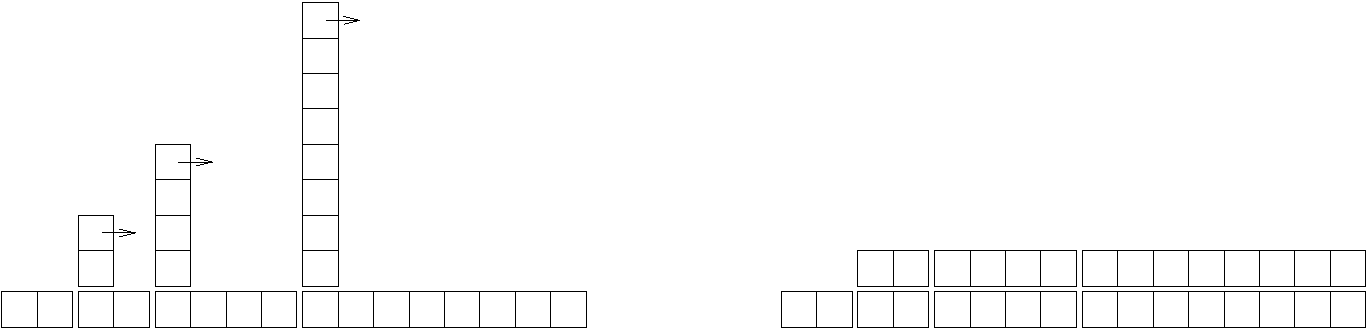
\includegraphics[scale=1.0]{figs/towers.pdf}}
\caption{The cost of a hashtable add.\label{fig.hash}}
\end{figure}

The extra work of rehashing appears as a sequence of increasingly
tall towers with increasing space between them.  Now if you knock
over the towers, amortizing the cost of resizing over all
adds, you can see graphically that the total cost after $n$
adds is $2n - 2$.

An important feature of this algorithm is that when we resize the
HashTable it grows geometrically; that is, we multiply the size by a
constant.  If you increase the size
arithmetically---adding a fixed number each time---the average time
per {\tt add} is linear.
\index{geometric resizing}

You can download my implementation of HashMap from
\url{http://thinkpython/code/Map.py}, but remember that there
is no reason to use it; if you want a map, just use a Python dictionary.






\chapter{Lumpy}
\label{lumpy}

Throughout the book, I have used diagrams to represent the state of
running programs.
\index{Lumpy}

In Section~\ref{variables}, we used a state diagram to show the names
and values of variables.  In Section~\ref{stackdiagram} I introduced a
stack diagram, which shows one frame for each function call.  Each
frame shows the parameters and local variables for the function or
method.  Stack diagrams for recursive functions appear in
Section~\ref{recursive.stack} and Section~\ref{more.recursion}.
\index{stack diagram} \index{diagram!stack}
\index{state diagram} \index{diagram!state}

Section~\ref{mutable} shows what a list looks like in a state diagram,
Section~\ref{invert} shows what a dictionary looks like, and
Section~\ref{dictuple} shows two ways to represent tuples.

Section~\ref{attributes} introduces object diagrams, which show the
state of an object's attributes, and their attributes, and so on.
Section~\ref{rectangles} has object diagrams for Rectangles and
their embedded Points.  Section~\ref{time.object} shows the state
of a Time object.
Section~\ref{class.attribute} has a diagram that includes a class
object and an instance, each with their own attributes.
\index{object diagram}
\index{diagram!object}

Finally, Section~\ref{class.diagram} introduces class diagrams,
which show the classes that make up a program and the relationships
between them.
\index{class diagram}
\index{diagram!class}

These diagrams are based on the Unified Modeling Language (UML), which
is a standardized graphical language used by software engineers
to communicate about program design, especially for object-oriented
programs.
\index{Unified Modeling Language}
\index{UML}

UML is a rich language with many kinds of diagrams that represent
many kinds of relationship between objects and classes.  What I presented
in this book is a small subset of the language, but it is the subset
most commonly used in practice.

The purpose of this appendix is to review the diagrams presented in
the previous chapters, and to introduce Lumpy.  Lumpy, which stands
for ``UML in Python,'' with some of the letters rearranged, is part of
Swampy, which you already installed if you worked on the case study in
Chapter~\ref{turtlechap} or Chapter~\ref{tkinter}, or if you did
Exercise~\ref{canvas},
\index{Lumpy}
\index{Swampy}

Lumpy uses Python's {\tt inspect} module to examine the state of a running
program and generate object diagrams (including stack diagrams) and
class diagrams.

\section{State diagram}

\begin{figure}
\centerline
{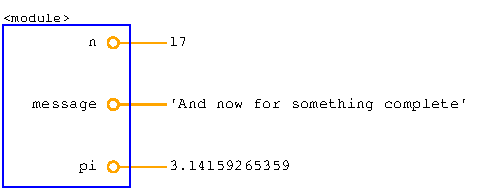
\includegraphics[scale=0.7]{figs/lumpydemo1.pdf}}
\caption{State diagram generated by Lumpy.}
\label{fig.lumpy1}
\end{figure}

Here's an example that uses Lumpy to generate a state diagram.
\index{state diagram} \index{diagram!state}

\begin{verbatim}
from swampy.Lumpy import Lumpy

lumpy = Lumpy()
lumpy.make_reference()

message = 'And now for something completely different'
n = 17
pi = 3.1415926535897932

lumpy.object_diagram()
\end{verbatim}

The first line imports the Lumpy class from {\tt swampy.Lumpy}.
If you don't have Swampy installed as a package, make sure
the Swampy files are in Python's search path and use this
{\tt import} statement instead:

\begin{verbatim}
from Lumpy import Lumpy
\end{verbatim}

The next lines create a {\tt Lumpy} object and make a ``reference''
point, which means that Lumpy records the objects that have been
defined so far.

Next we define new variables and invoke \verb"object_diagram",
which draws the objects that have been defined since the reference
point, in this case {\tt message}, {\tt n} and {\tt pi}.

Figure~\ref{fig.lumpy1} shows the result.  The graphical style is
different from what I showed earlier; for example, each
reference is represented by a circle next to the variable name and a
line to the value.  And long strings are truncated.  But the
information conveyed by the diagram is the same.

The variable names are in a frame labeled \verb"<module>", which
indicates that these are module-level variables, also known as
global.
\index{global variable}
\index{variable!global}
\index{module-level variable}
\index{variable!module-level}

You can download this example from
\url{http://thinkpython.com/code/lumpy_demo1.py}.  Try adding some
additional assignments and see what the diagram looks like.


\section{Stack diagram}

\begin{figure}
\centerline
{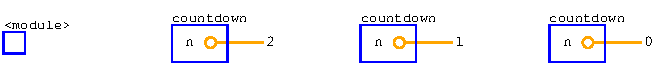
\includegraphics[scale=0.7]{figs/lumpydemo2.pdf}}
\caption{Stack diagram.}
\label{fig.lumpy2}
\end{figure}

Here's an example that uses Lumpy to generate a stack diagram.
You can download it from \url{http://thinkpython.com/code/lumpy_demo2.py}.
\index{stack diagram} \index{diagram!stack}

\begin{verbatim}
from swampy.Lumpy import Lumpy

def countdown(n):
    if n <= 0:
        print 'Blastoff!'
        lumpy.object_diagram()
    else:
        print n
        countdown(n-1)

lumpy = Lumpy()
lumpy.make_reference()
countdown(3)
\end{verbatim}

Figure~\ref{fig.lumpy2} shows the result.  Each frame is represented
with a box that has the function's name outside and variables inside.
Since this function is recursive, there is one frame for each
level of recursion.
\index{recursion}
\index{function frame}
\index{frame}

Remember that a stack diagram shows the state of the program at
a particular point in its execution.  To get the diagram you want,
sometimes you have to think about where to invoke \verb"object_diagram".

In this case I invoke \verb"object_diagram" after executing the base
case of the recursion; that way the stack diagram shows each level of
the recursion.  You can call \verb"object_diagram" more than once to
get a series of snapshots of the program's execution.
\index{base case}


\section{Object diagrams}

\begin{figure}
\centerline
{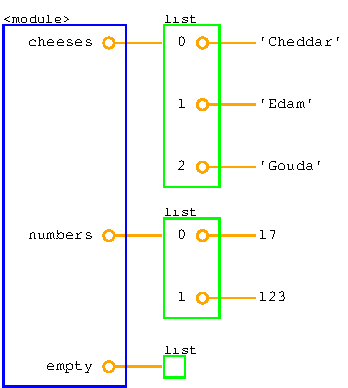
\includegraphics[scale=0.7]{figs/lumpydemo3.pdf}}
\caption{Object diagram.}
\label{fig.lumpy3}
\end{figure}

This example generates an object diagram showing the lists from
Section~\ref{sequence}.  You can download it from
\url{http://thinkpython.com/code/lumpy_demo3.py}.
\index{object diagram} \index{diagram!object}

\begin{verbatim}
from swampy.Lumpy import Lumpy

lumpy = Lumpy()
lumpy.make_reference()

cheeses = ['Cheddar', 'Edam', 'Gouda']
numbers = [17, 123]
empty = []

lumpy.object_diagram()
\end{verbatim}

Figure~\ref{fig.lumpy3} shows the result.  Lists are represented by
a box that shows the indices mapping to the elements.  This representation
is slightly misleading, since indices are not actually
part of the list, but I think they make the diagram easier to
read.  The empty list is represented by an empty box.
\index{list index}

\begin{figure}
\centerline
{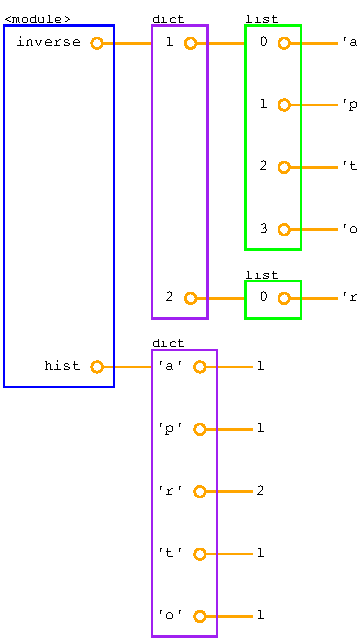
\includegraphics[scale=0.7]{figs/lumpydemo4.pdf}}
\caption{Object diagram.}
\label{fig.lumpy4}
\end{figure}

And here's an example
showing the dictionaries from Section~\ref{invert}.  You can download
it from \url{http://thinkpython.com/code/lumpy_demo4.py}.
\index{dictionary}

\begin{verbatim}
from swampy.Lumpy import Lumpy

lumpy = Lumpy()
lumpy.make_reference()

hist = histogram('parrot')
inverse = invert_dict(hist)

lumpy.object_diagram()
\end{verbatim}

Figure~\ref{fig.lumpy4} shows the result.  {\tt hist} is a dictionary
that maps from characters (single-letter strings) to integers;
{\tt inverse} maps from integers to lists of strings.

\begin{figure}
\centerline
{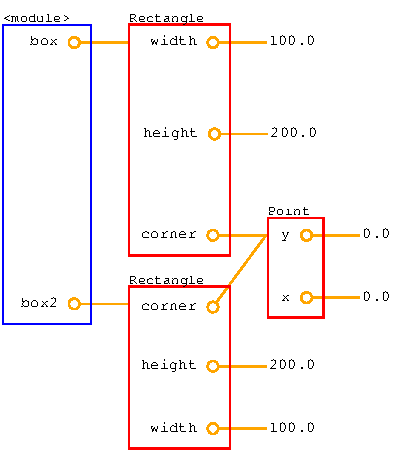
\includegraphics[scale=0.7]{figs/lumpydemo5.pdf}}
\caption{Object diagram.}
\label{fig.lumpy5}
\end{figure}

This example generates an object diagram for Point and Rectangle
objects, as in Section~\ref{copying}.  You can download it from
\url{http://thinkpython.com/code/lumpy_demo5.py}.
\index{Point class}
\index{class!Point}
\index{Rectangle class}
\index{class!Rectangle}

\begin{verbatim}
import copy
from swampy.Lumpy import Lumpy

lumpy = Lumpy()
lumpy.make_reference()

box = Rectangle()
box.width = 100.0
box.height = 200.0
box.corner = Point()
box.corner.x = 0.0
box.corner.y = 0.0

box2 = copy.copy(box)

lumpy.object_diagram()
\end{verbatim}

Figure~\ref{fig.lumpy5} shows the result.  {\tt copy.copy} make a
shallow copy, so {\tt box} and {\tt box2} have their own {\tt width}
and {\tt height}, but they share the same embedded Point object.  This
kind of sharing is usually fine with immutable objects, but with
mutable types, it is highly error-prone.
\index{copy}
\index{shallow copy}

\section{Function and class objects}

\begin{figure}
\centerline
{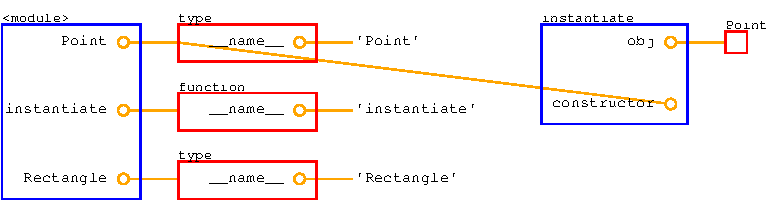
\includegraphics[scale=0.7]{figs/lumpydemo6.pdf}}
\caption{Object diagram.}
\label{fig.lumpy6}
\end{figure}

When I use Lumpy to make object diagrams, I usually define the functions
and classes before I make the reference point.  That way, function
and class objects don't appear in the diagram.
\index{function object}
\index{object!function}
\index{class object}
\index{object!class}

But if you are passing functions and classes as parameters, you might
want them to appear.  This example shows what that looks like;
you can download it from
\url{http://thinkpython.com/code/lumpy_demo6.py}.

\begin{verbatim}
import copy
from swampy.Lumpy import Lumpy

lumpy = Lumpy()
lumpy.make_reference()

class Point(object):
    """Represents a point in 2-D space."""

class Rectangle(object):
    """Represents a rectangle."""

def instantiate(constructor):
    """Instantiates a new object."""
    obj = constructor()
    lumpy.object_diagram()
    return obj

point = instantiate(Point)
\end{verbatim}

Figure~\ref{fig.lumpy6} shows the result.  Since we invoke
\verb"object_diagram" inside a function, we get a stack diagram
with a frame for the module-level variables and for the invocation
of {\tt instantiate}.

At the module level, {\tt Point} and {\tt Rectangle} refer to
class objects (which have type {\tt type}); {\tt instantiate}
refers to a function object.
\index{instantiate}
\index{constructor}

This diagram might clarify two points of common confusion: (1) the
difference between the class object, {\tt Point}, and the instance of
Point, {\tt obj}, and (2) the difference between the function object
created when {\tt instantiate} is defined, and the frame created with
it is called.


\section{Class Diagrams}

\begin{figure}
\centerline
{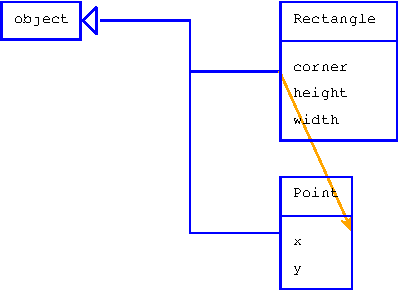
\includegraphics[scale=0.7]{figs/lumpydemo7.pdf}}
\caption{Class diagram.}
\label{fig.lumpy7}
\end{figure}

\begin{figure}
\centerline
{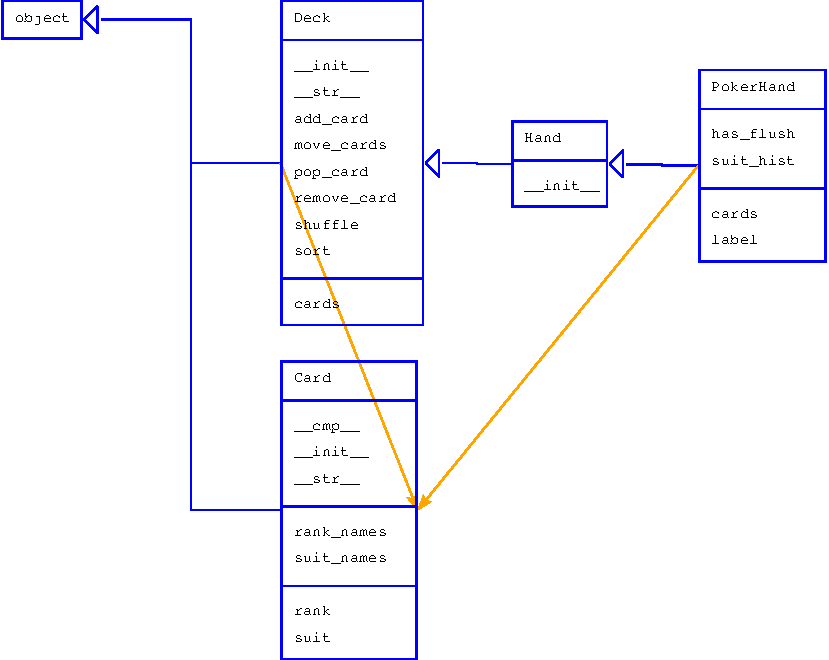
\includegraphics[scale=0.7]{figs/lumpydemo8.pdf}}
\caption{Class diagram.}
\label{fig.lumpy8}
\end{figure}

Although I distinguish between state diagrams, stack diagrams and
object diagrams, they are mostly the same thing: they show the
state of a running program at a point in time.
\index{class diagram}
\index{diagram!class}

Class diagrams are different.  They show the classes that make up a
program and the relationships between them.  They are timeless in the
sense that they describe the program as a whole, not any particular
point in time.  For example, if an instance of Class A generally
contains a reference to an instance of Class B, we say there is a
``HAS-A relationship'' between those classes.
\index{HAS-A relationship}
\index{class diagram}
\index{diagram!class}
\index{UML}

Here's an example that shows a HAS-A relationship.  You can download
it from \url{http://thinkpython.com/code/lumpy_demo7.py}.

\begin{verbatim}
from swampy.Lumpy import Lumpy

lumpy = Lumpy()
lumpy.make_reference()

box = Rectangle()
box.width = 100.0
box.height = 200.0
box.corner = Point()
box.corner.x = 0.0
box.corner.y = 0.0

lumpy.class_diagram()
\end{verbatim}

Figure~\ref{fig.lumpy7} shows the result.
Each class is represented with a box that contains the name of the
class, any methods the class provides, any class variables, and
any instance variables.  In this example, {\tt Rectangle} and {\tt Point}
have instance variables, but no methods or class variables.

The arrow from {\tt Rectangle} to {\tt Point} shows that Rectangles
contain an embedded Point.  In addition, {\tt Rectangle} and {\tt
  Point} both inherit from {\tt object}, which is represented in
the diagram with a triangle-headed arrow.
\index{IS-A relationship}

Here's a more complex example using my solution to Exercise~\ref{poker}.
You can download
the code from \url{http://thinkpython.com/code/lumpy_demo8.py};
you will also need \url{http://thinkpython.com/code/PokerHand.py}.

\begin{verbatim}
from swampy.Lumpy import Lumpy

from PokerHand import *

lumpy = Lumpy()
lumpy.make_reference()

deck = Deck()
hand = PokerHand()
deck.move_cards(hand, 7)

lumpy.class_diagram()
\end{verbatim}

Figure~\ref{fig.lumpy8} shows the result.
{\tt PokerHand} inherits from {\tt Hand}, which inherits from {\tt Deck}.
Both {\tt Deck} and {\tt PokerHand} have Cards.
\index{Card class}
\index{Deck class}
\index{Hand class}

This diagram does not show that {\tt Hand} also has cards, because
in the program there are no instances of Hand.  This example
demonstrates a limitation of Lumpy; it only knows about the
attributes and HAS-A relationships of objects that are instantiated.

\printindex

\clearemptydoublepage
%\blankpage
%\blankpage
%\blankpage


\end{document}
